% Options for packages loaded elsewhere
\PassOptionsToPackage{unicode}{hyperref}
\PassOptionsToPackage{hyphens}{url}
\PassOptionsToPackage{dvipsnames,svgnames,x11names}{xcolor}
%
\documentclass[
  letterpaper,
  DIV=11,
  numbers=noendperiod]{scrreprt}

\usepackage{amsmath,amssymb}
\usepackage{iftex}
\ifPDFTeX
  \usepackage[T1]{fontenc}
  \usepackage[utf8]{inputenc}
  \usepackage{textcomp} % provide euro and other symbols
\else % if luatex or xetex
  \usepackage{unicode-math}
  \defaultfontfeatures{Scale=MatchLowercase}
  \defaultfontfeatures[\rmfamily]{Ligatures=TeX,Scale=1}
\fi
\usepackage{lmodern}
\ifPDFTeX\else  
    % xetex/luatex font selection
\fi
% Use upquote if available, for straight quotes in verbatim environments
\IfFileExists{upquote.sty}{\usepackage{upquote}}{}
\IfFileExists{microtype.sty}{% use microtype if available
  \usepackage[]{microtype}
  \UseMicrotypeSet[protrusion]{basicmath} % disable protrusion for tt fonts
}{}
\makeatletter
\@ifundefined{KOMAClassName}{% if non-KOMA class
  \IfFileExists{parskip.sty}{%
    \usepackage{parskip}
  }{% else
    \setlength{\parindent}{0pt}
    \setlength{\parskip}{6pt plus 2pt minus 1pt}}
}{% if KOMA class
  \KOMAoptions{parskip=half}}
\makeatother
\usepackage{xcolor}
\setlength{\emergencystretch}{3em} % prevent overfull lines
\setcounter{secnumdepth}{-\maxdimen} % remove section numbering
% Make \paragraph and \subparagraph free-standing
\makeatletter
\ifx\paragraph\undefined\else
  \let\oldparagraph\paragraph
  \renewcommand{\paragraph}{
    \@ifstar
      \xxxParagraphStar
      \xxxParagraphNoStar
  }
  \newcommand{\xxxParagraphStar}[1]{\oldparagraph*{#1}\mbox{}}
  \newcommand{\xxxParagraphNoStar}[1]{\oldparagraph{#1}\mbox{}}
\fi
\ifx\subparagraph\undefined\else
  \let\oldsubparagraph\subparagraph
  \renewcommand{\subparagraph}{
    \@ifstar
      \xxxSubParagraphStar
      \xxxSubParagraphNoStar
  }
  \newcommand{\xxxSubParagraphStar}[1]{\oldsubparagraph*{#1}\mbox{}}
  \newcommand{\xxxSubParagraphNoStar}[1]{\oldsubparagraph{#1}\mbox{}}
\fi
\makeatother


\providecommand{\tightlist}{%
  \setlength{\itemsep}{0pt}\setlength{\parskip}{0pt}}\usepackage{longtable,booktabs,array}
\usepackage{calc} % for calculating minipage widths
% Correct order of tables after \paragraph or \subparagraph
\usepackage{etoolbox}
\makeatletter
\patchcmd\longtable{\par}{\if@noskipsec\mbox{}\fi\par}{}{}
\makeatother
% Allow footnotes in longtable head/foot
\IfFileExists{footnotehyper.sty}{\usepackage{footnotehyper}}{\usepackage{footnote}}
\makesavenoteenv{longtable}
\usepackage{graphicx}
\makeatletter
\newsavebox\pandoc@box
\newcommand*\pandocbounded[1]{% scales image to fit in text height/width
  \sbox\pandoc@box{#1}%
  \Gscale@div\@tempa{\textheight}{\dimexpr\ht\pandoc@box+\dp\pandoc@box\relax}%
  \Gscale@div\@tempb{\linewidth}{\wd\pandoc@box}%
  \ifdim\@tempb\p@<\@tempa\p@\let\@tempa\@tempb\fi% select the smaller of both
  \ifdim\@tempa\p@<\p@\scalebox{\@tempa}{\usebox\pandoc@box}%
  \else\usebox{\pandoc@box}%
  \fi%
}
% Set default figure placement to htbp
\def\fps@figure{htbp}
\makeatother

\KOMAoption{captions}{tableheading}
\makeatletter
\@ifpackageloaded{tcolorbox}{}{\usepackage[skins,breakable]{tcolorbox}}
\@ifpackageloaded{fontawesome5}{}{\usepackage{fontawesome5}}
\definecolor{quarto-callout-color}{HTML}{909090}
\definecolor{quarto-callout-note-color}{HTML}{0758E5}
\definecolor{quarto-callout-important-color}{HTML}{CC1914}
\definecolor{quarto-callout-warning-color}{HTML}{EB9113}
\definecolor{quarto-callout-tip-color}{HTML}{00A047}
\definecolor{quarto-callout-caution-color}{HTML}{FC5300}
\definecolor{quarto-callout-color-frame}{HTML}{acacac}
\definecolor{quarto-callout-note-color-frame}{HTML}{4582ec}
\definecolor{quarto-callout-important-color-frame}{HTML}{d9534f}
\definecolor{quarto-callout-warning-color-frame}{HTML}{f0ad4e}
\definecolor{quarto-callout-tip-color-frame}{HTML}{02b875}
\definecolor{quarto-callout-caution-color-frame}{HTML}{fd7e14}
\makeatother
\makeatletter
\@ifpackageloaded{caption}{}{\usepackage{caption}}
\AtBeginDocument{%
\ifdefined\contentsname
  \renewcommand*\contentsname{Table of contents}
\else
  \newcommand\contentsname{Table of contents}
\fi
\ifdefined\listfigurename
  \renewcommand*\listfigurename{List of Figures}
\else
  \newcommand\listfigurename{List of Figures}
\fi
\ifdefined\listtablename
  \renewcommand*\listtablename{List of Tables}
\else
  \newcommand\listtablename{List of Tables}
\fi
\ifdefined\figurename
  \renewcommand*\figurename{Figure}
\else
  \newcommand\figurename{Figure}
\fi
\ifdefined\tablename
  \renewcommand*\tablename{Table}
\else
  \newcommand\tablename{Table}
\fi
}
\@ifpackageloaded{float}{}{\usepackage{float}}
\floatstyle{ruled}
\@ifundefined{c@chapter}{\newfloat{codelisting}{h}{lop}}{\newfloat{codelisting}{h}{lop}[chapter]}
\floatname{codelisting}{Listing}
\newcommand*\listoflistings{\listof{codelisting}{List of Listings}}
\makeatother
\makeatletter
\makeatother
\makeatletter
\@ifpackageloaded{caption}{}{\usepackage{caption}}
\@ifpackageloaded{subcaption}{}{\usepackage{subcaption}}
\makeatother

\usepackage{bookmark}

\IfFileExists{xurl.sty}{\usepackage{xurl}}{} % add URL line breaks if available
\urlstyle{same} % disable monospaced font for URLs
\hypersetup{
  pdftitle={Little Kids, Big Adventures: A Guide to Family Hikes Around Knoxville},
  pdfauthor={Katie Rosenberg and Joshua Rosenberg},
  colorlinks=true,
  linkcolor={blue},
  filecolor={Maroon},
  citecolor={Blue},
  urlcolor={Blue},
  pdfcreator={LaTeX via pandoc}}


\title{Little Kids, Big Adventures: A Guide to Family Hikes Around
Knoxville}
\usepackage{etoolbox}
\makeatletter
\providecommand{\subtitle}[1]{% add subtitle to \maketitle
  \apptocmd{\@title}{\par {\large #1 \par}}{}{}
}
\makeatother
\subtitle{The Tennessee Valley, Cumberland Plateau, and Great Smoky
Mountains National Park}
\author{Katie Rosenberg and Joshua Rosenberg}
\date{2025-02-01}

\begin{document}
\maketitle

\renewcommand*\contentsname{Table of contents}
{
\hypersetup{linkcolor=}
\setcounter{tocdepth}{2}
\tableofcontents
}

\chapter{Preface}\label{preface}

\subsection{A story about a hike}\label{a-story-about-a-hike}

\begin{tcolorbox}[enhanced jigsaw, colback=white, colframe=quarto-callout-warning-color-frame, breakable, opacityback=0, toprule=.15mm, bottomrule=.15mm, rightrule=.15mm, left=2mm, leftrule=.75mm, arc=.35mm]
\begin{minipage}[t]{5.5mm}
\textcolor{quarto-callout-warning-color}{\faExclamationTriangle}
\end{minipage}%
\begin{minipage}[t]{\textwidth - 5.5mm}

Please note - this book is in-progress and many sections are not yet
drafted or are in draft form! It is set to be published by
\href{https://utpress.org/}{UT Press} with an expected publication date
in early 2026.

\end{minipage}%
\end{tcolorbox}

\begin{figure}[H]

{\centering \pandocbounded{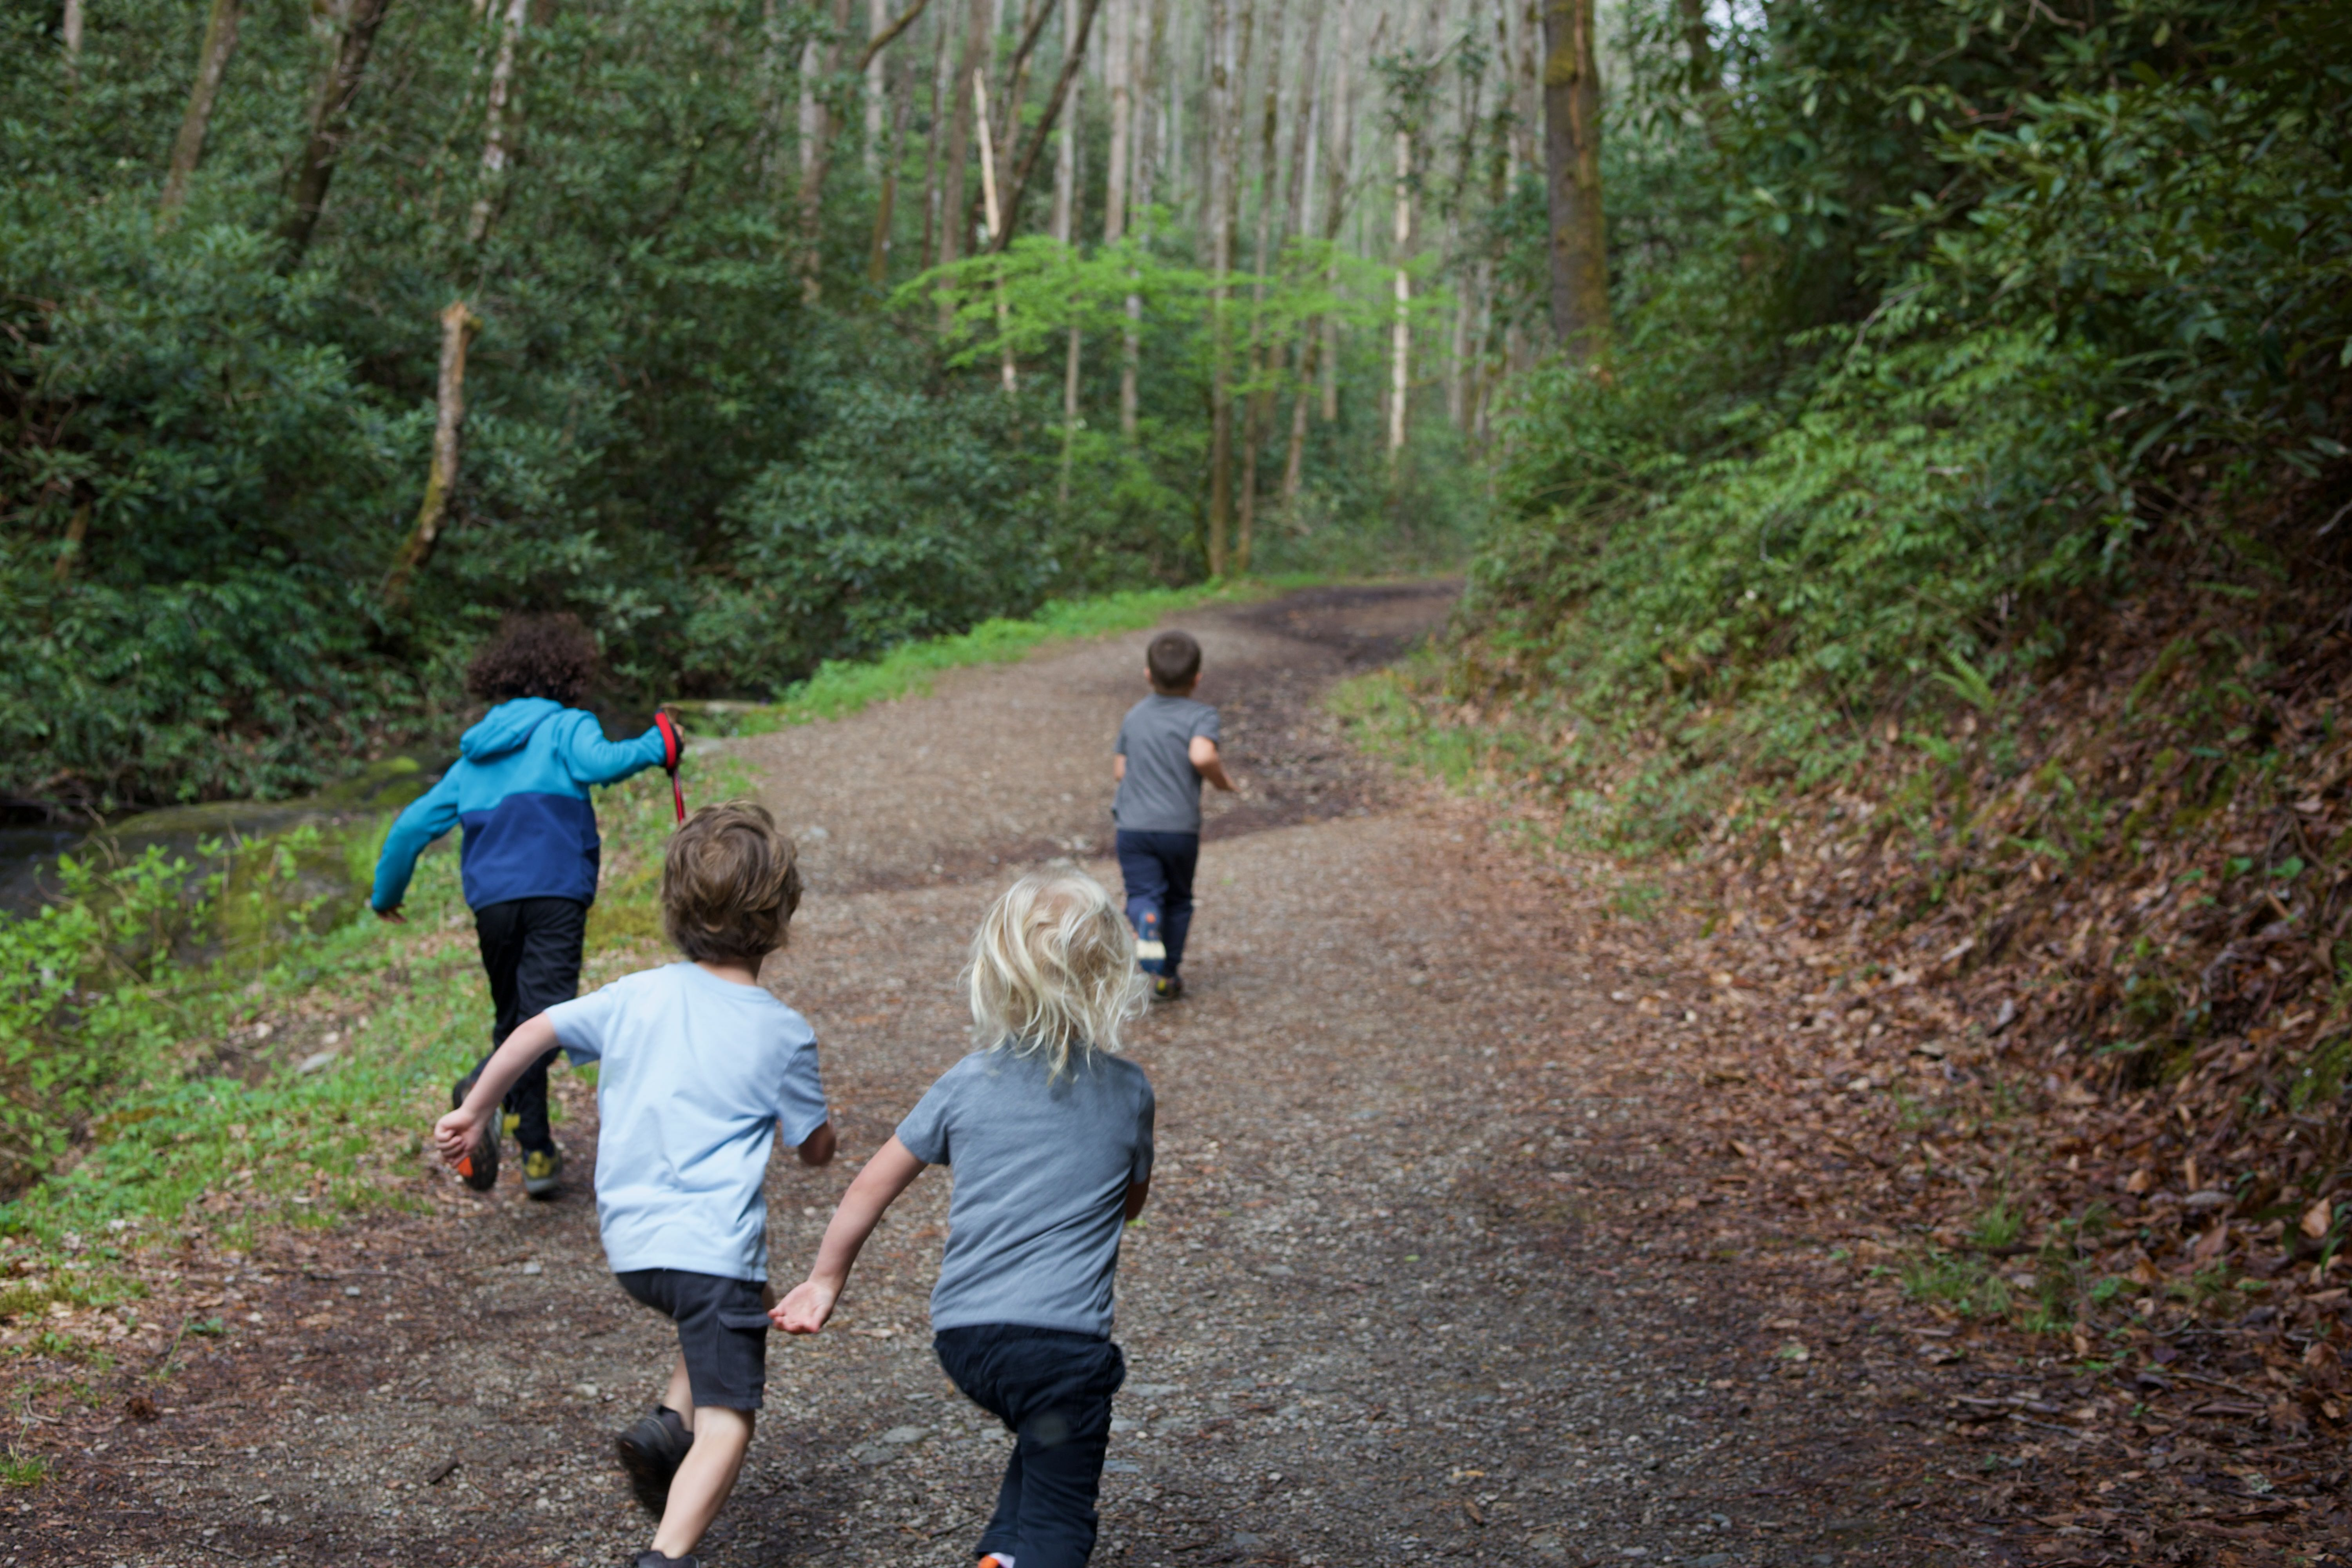
\includegraphics[keepaspectratio]{img/trail-23-figure-02.jpg}}

}

\caption{Photo credit to Katie and Joshua Rosenberg}

\end{figure}%

Picture this: A sunny day in nature with your family. Your kids happily
climb up and over rocks, stopping only to splash in creeks. At the end,
you have a picnic on the grass on a perfect, mild but warm day without a
bug to be found.

\emph{Record Scratch}

Sure, we'd all love for the above vision to be reality, but the truth is
almost always a bit messier and with unexpected bumps in the road.

If you're like us, you might be ready to throw in the towel before you
even leave home. We've been there.

However, we've also grown as a family who hikes, homed on the process,
and adjusted our expectations. And sometimes the weather is just right,
we and the kiddos are having a great time, and, every once in a while,
there really isn't a bug in sight.

\begin{figure}[H]

{\centering \pandocbounded{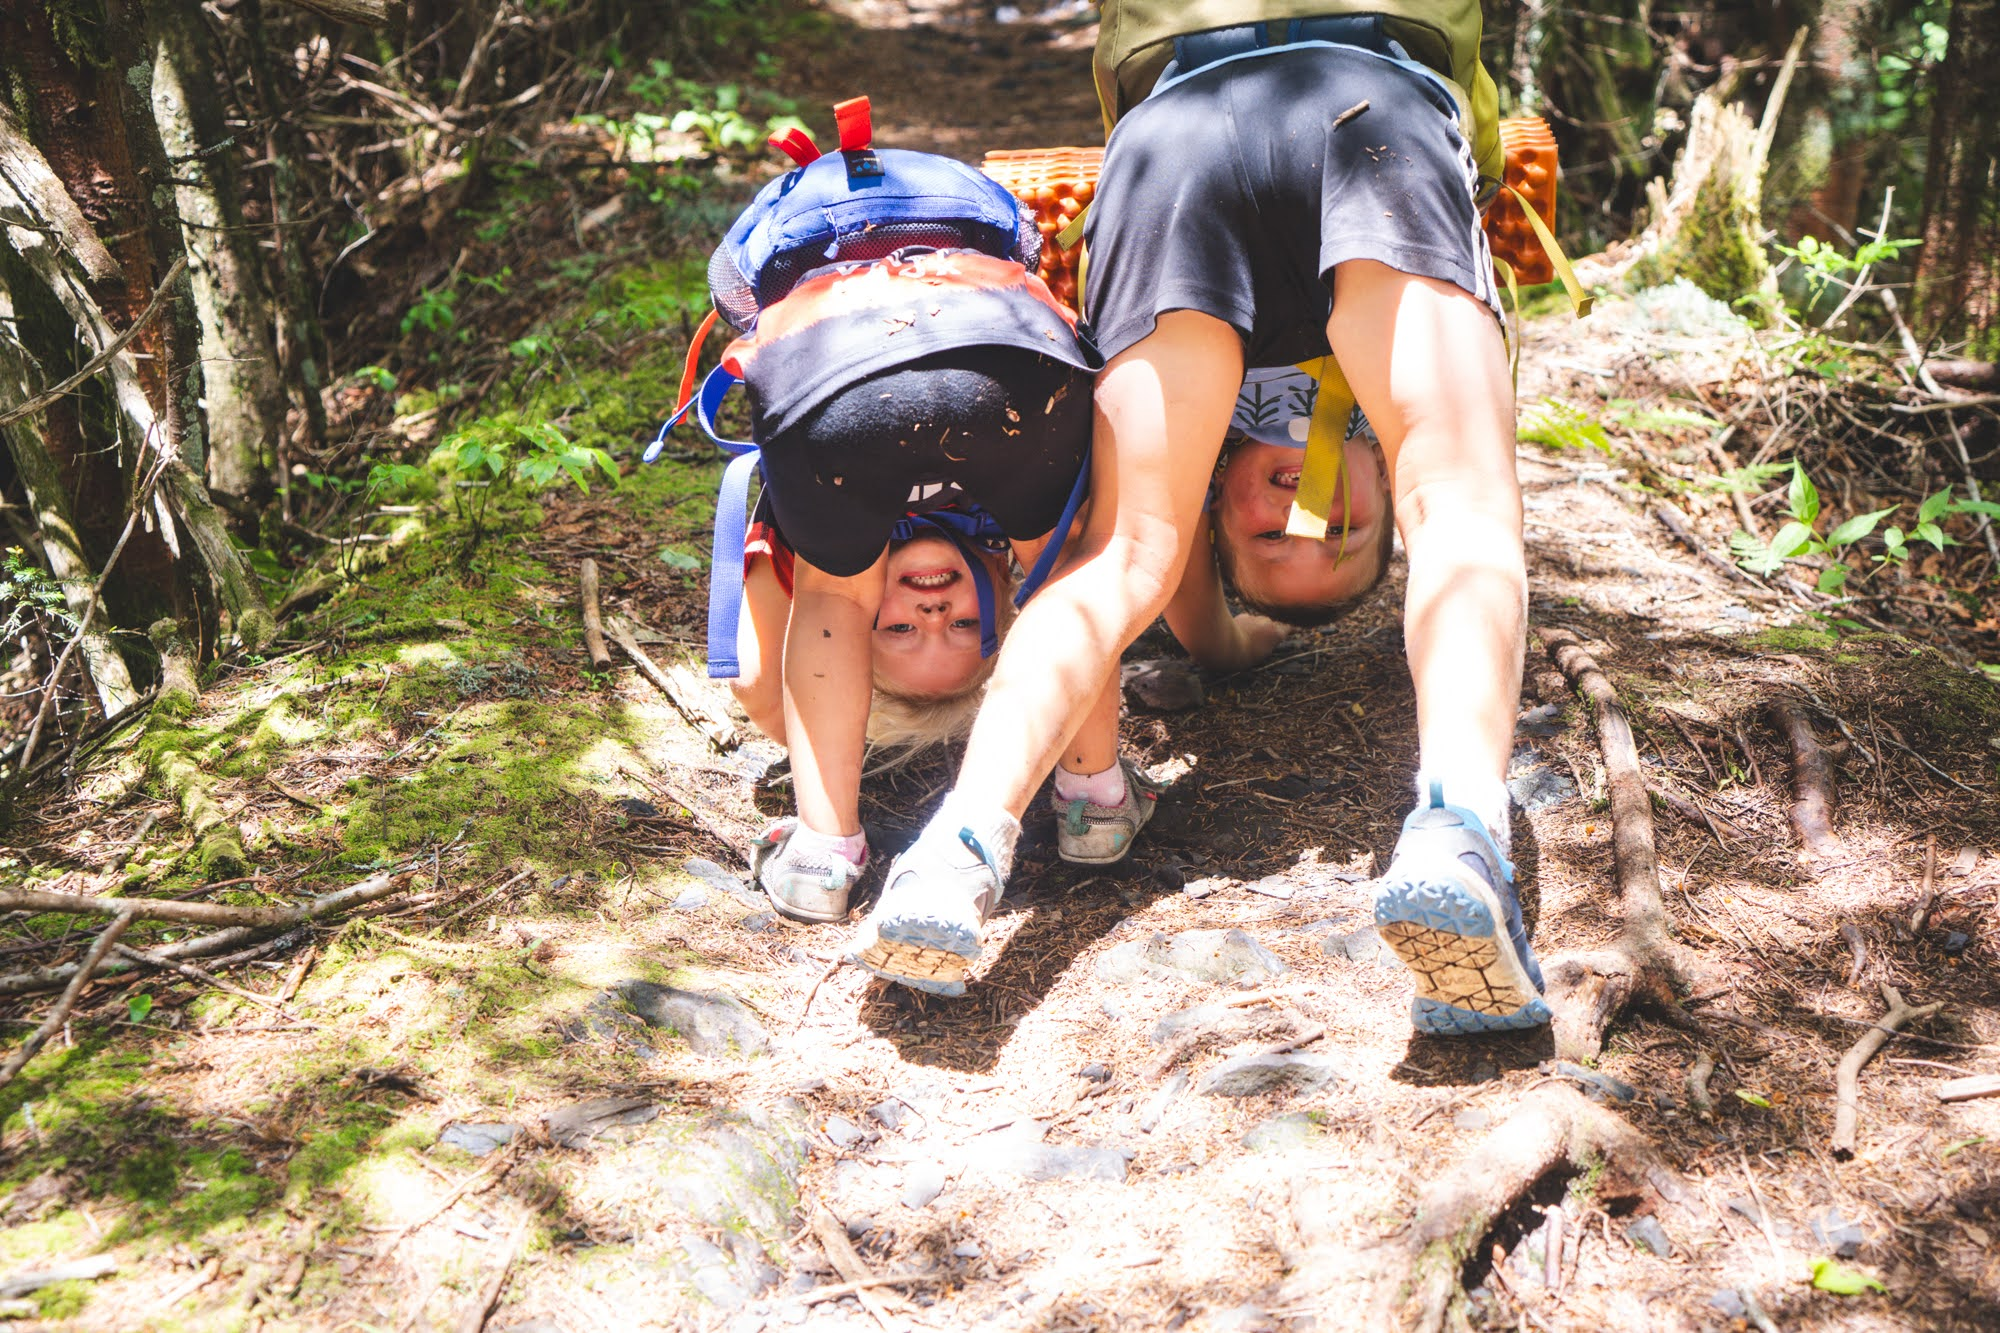
\includegraphics[keepaspectratio]{img/ruth-levi.jpg}}

}

\caption{Photo credit to Sam Weisbrod}

\end{figure}%

\subsection{We wrote this to help our friends (and
you!)}\label{we-wrote-this-to-help-our-friends-and-you}

After moving to Knoxville as a very young famiy in 2018, our first trip
to Ijams introduced us to Knoxville's incredible outdoor spaces. A
camping trip at Frozen Head opened our eyes. Later, visiting the Smokies
sealed the deal: hiking helped us to feel connected to and later to love
where we live.

We don't think we're very special in this respect (and in most others!):
One of the many joys of writing this book was discovering that we'd
hiked all 30 of the trails in it.

As we transitioned from newcomers to becoming established, we were
increasingly asked questions by our friends:

\emph{Where should we hike with our kids?}

and

\emph{What do I need to hike with our kids?}

This book is meant to answer those questions. But, as a sneak preview,
we picked out 30 trails with an eye not only toward the trails that are
scenic and exciting, but also those that are likely to balance driving
distance, crowds, and kid-friendly characteristics. And, one of the many
great parts about hiking is that you don't need much to get started.
Indeed, you may not need anything at all.

\subsection{Whom this book is for}\label{whom-this-book-is-for}

This book is for families and others caring for children who are looking
for an accessible introduction to getting started hiking around
Knoxville. Furthermore, this book is also for those with a few favorite
trails looking to do and learn more---find longer, more challenging
hikes or be introduced to hidden gems.

Because this book is for those new to hiking and those with some mud on
their shoes, we've included a wide range of hikes, from those shorter
than a mile on paved trails to epic expeditions into the Smokies.
Additionally, we've noted trails that are stroller-friendly or
accessible for families with additional needs.

\begin{figure}[H]

{\centering \pandocbounded{\includegraphics[keepaspectratio]{img/ayla-flowers.jpg}}

}

\caption{Photo credit to Katie and Joshua Rosenberg}

\end{figure}%

\subsection{Where the hikes are}\label{where-the-hikes-are}

All of the hikes are near Knoxville---from just a few minutes to within
an hour or two drive (but no longer). Following our focus on hiking with
younger children, most of the hikes are within an hour's drive of
Knoxville.

They are in three regions:

\begin{itemize}
\tightlist
\item
  \textbf{In and around Knoxville}: Hikes within the Knoxville city
  limits to those within a 30-minute drive.
\item
  \textbf{The Cumberland Plateau}: An often under-appreciated but
  fantastic region of rock outcroppings and wild rivers to the West and
  North of Knoxville. The hikes in this region are from around one to
  two hours from Knoxville, with most being close to one hour.
\item
  \textbf{The Great Smoky Mountains National Park}: The most-visited and
  the most biodiverse national park---right in Knoxville's backyard.
  These are mostly around an hour from Knoxville, though a few are
  closer to two hours.
\end{itemize}

\part{Introduction}

\chapter{Getting Ready for Your First
Hike}\label{getting-ready-for-your-first-hike}

\subsection{You don't need fancy gear!}\label{you-dont-need-fancy-gear}

There's a little secret in the hiking world. You don't need a lot to get
started. Indeed, you may not need anything \emph{new} at all.

Our view is that you don't need anything special to enjoy your first
hike. With the right trail and a few basics, you'll be ready for an
adventure.

First, though, there's another little secret we need to share.

\subsection{You don't need to be an experienced hiker to hike with
little
ones}\label{you-dont-need-to-be-an-experienced-hiker-to-hike-with-little-ones}

Hiking can be different from other physical activities in that it is not
a competition. Instead, it is about experiencing the outdoors in our own
way.

This applies to beginners and to the most experienced hikers; a common
saying shared among long-distance hikers is to \emph{hike your own
hike.} This means that each person hiking will hike in their way, and
that there is not anything like a correct way to lace up your shoes and
to get outdoors with your family. If this applies to long-distance
hikers, we think it doubly applies to families hiking with littles! Hike
your own hike.

\begin{figure}[H]

{\centering \pandocbounded{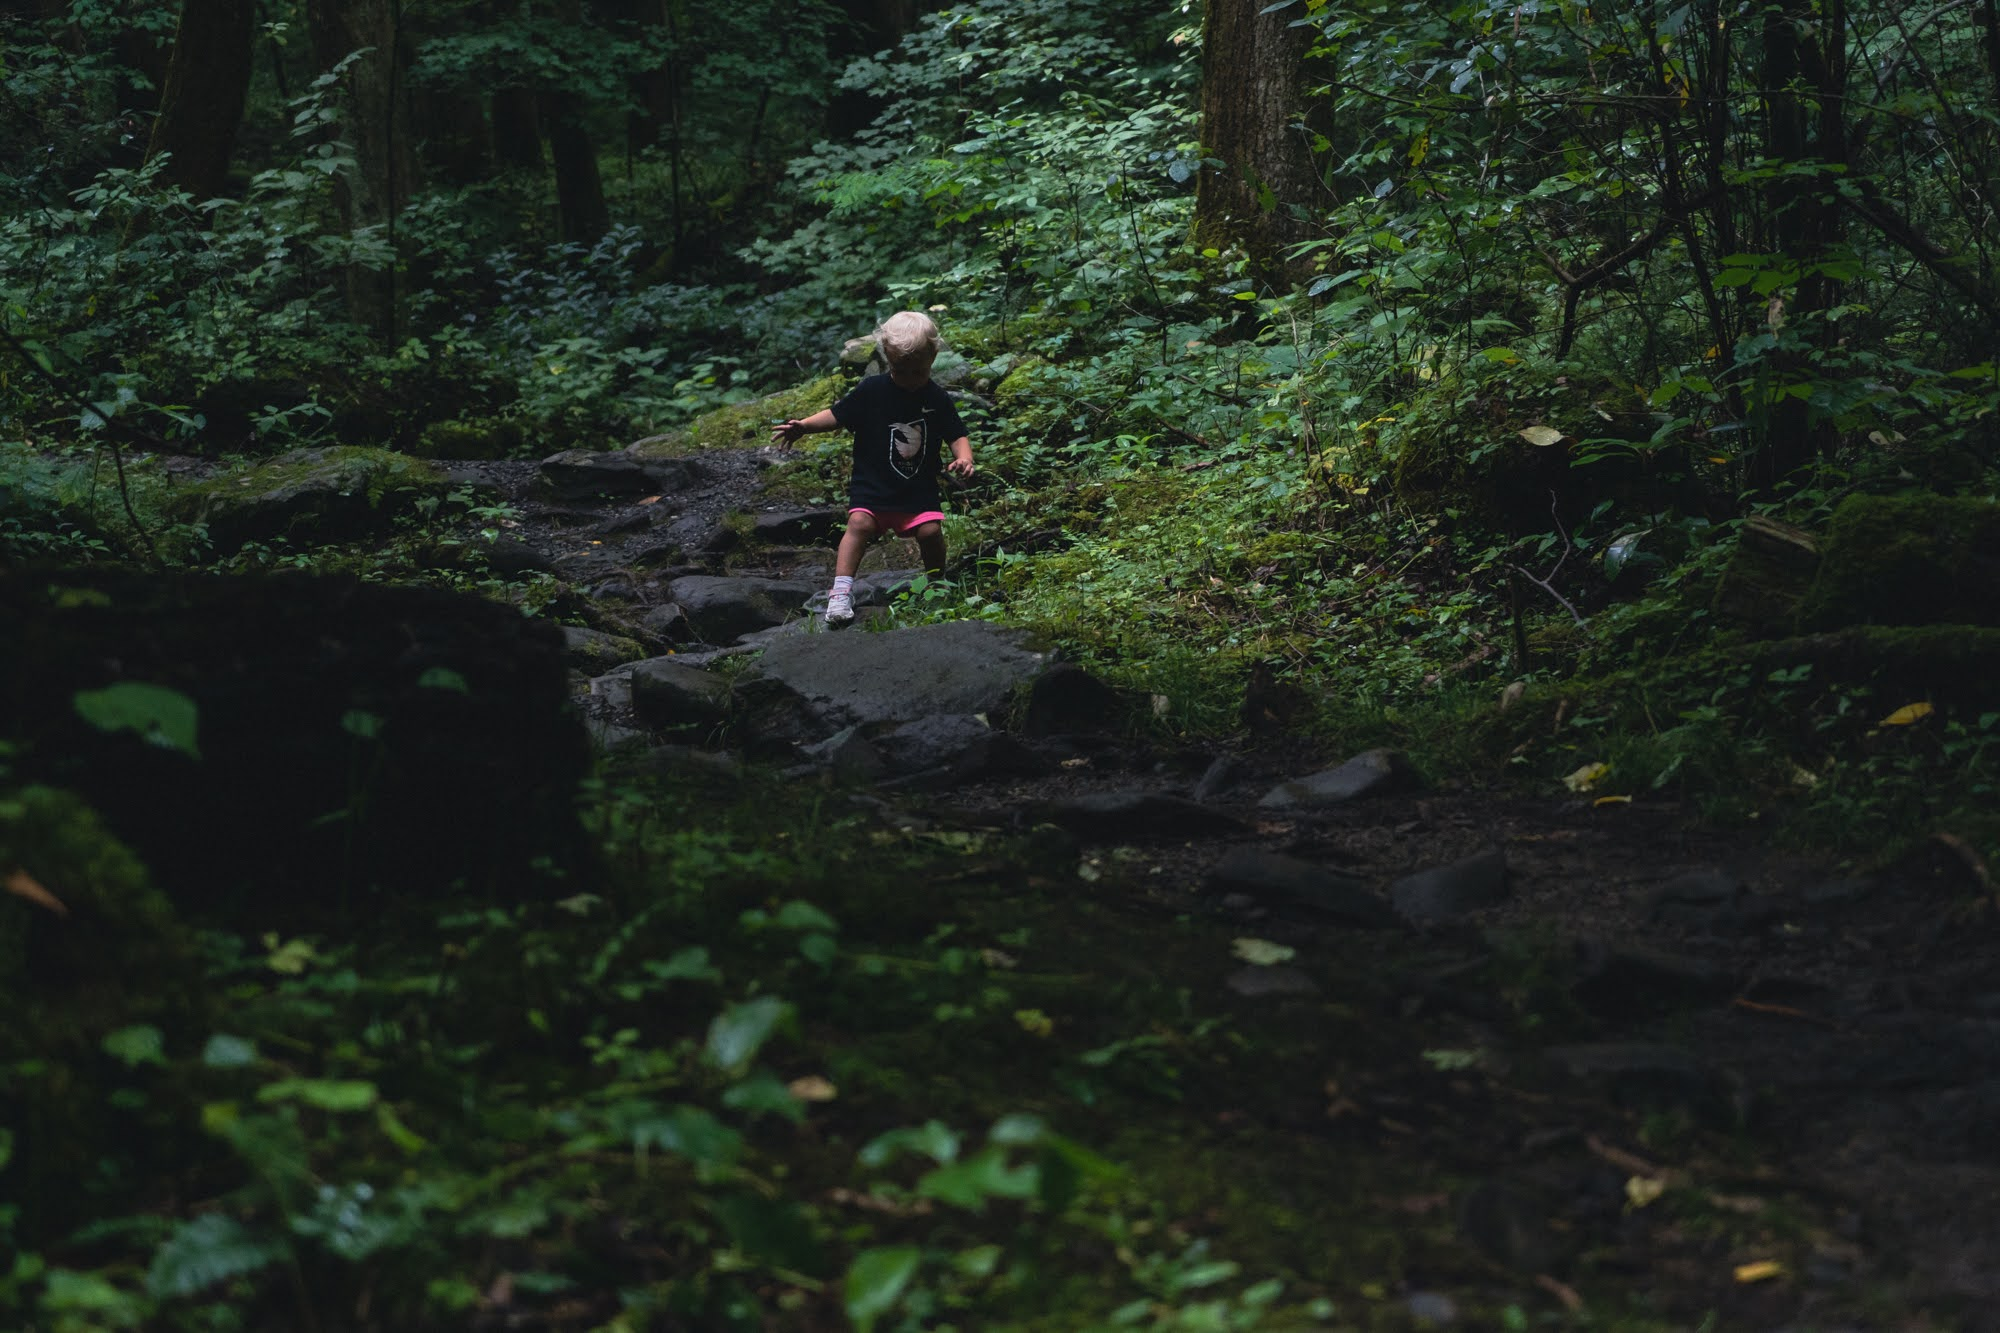
\includegraphics[keepaspectratio]{img/ruth-hill.jpg}}

}

\caption{Photo Credit to Sam Weisbrod}

\end{figure}%

\subsection{Let kids take the lead}\label{let-kids-take-the-lead}

To help your kids develop a love for hiking and the outdoors, let them
take the lead. Let them develop their own interests and explore their
own curiosities when you go on a hike. Sometimes this might mean playing
in a creek for half of your planned hiking time.

\begin{figure}[H]

{\centering \pandocbounded{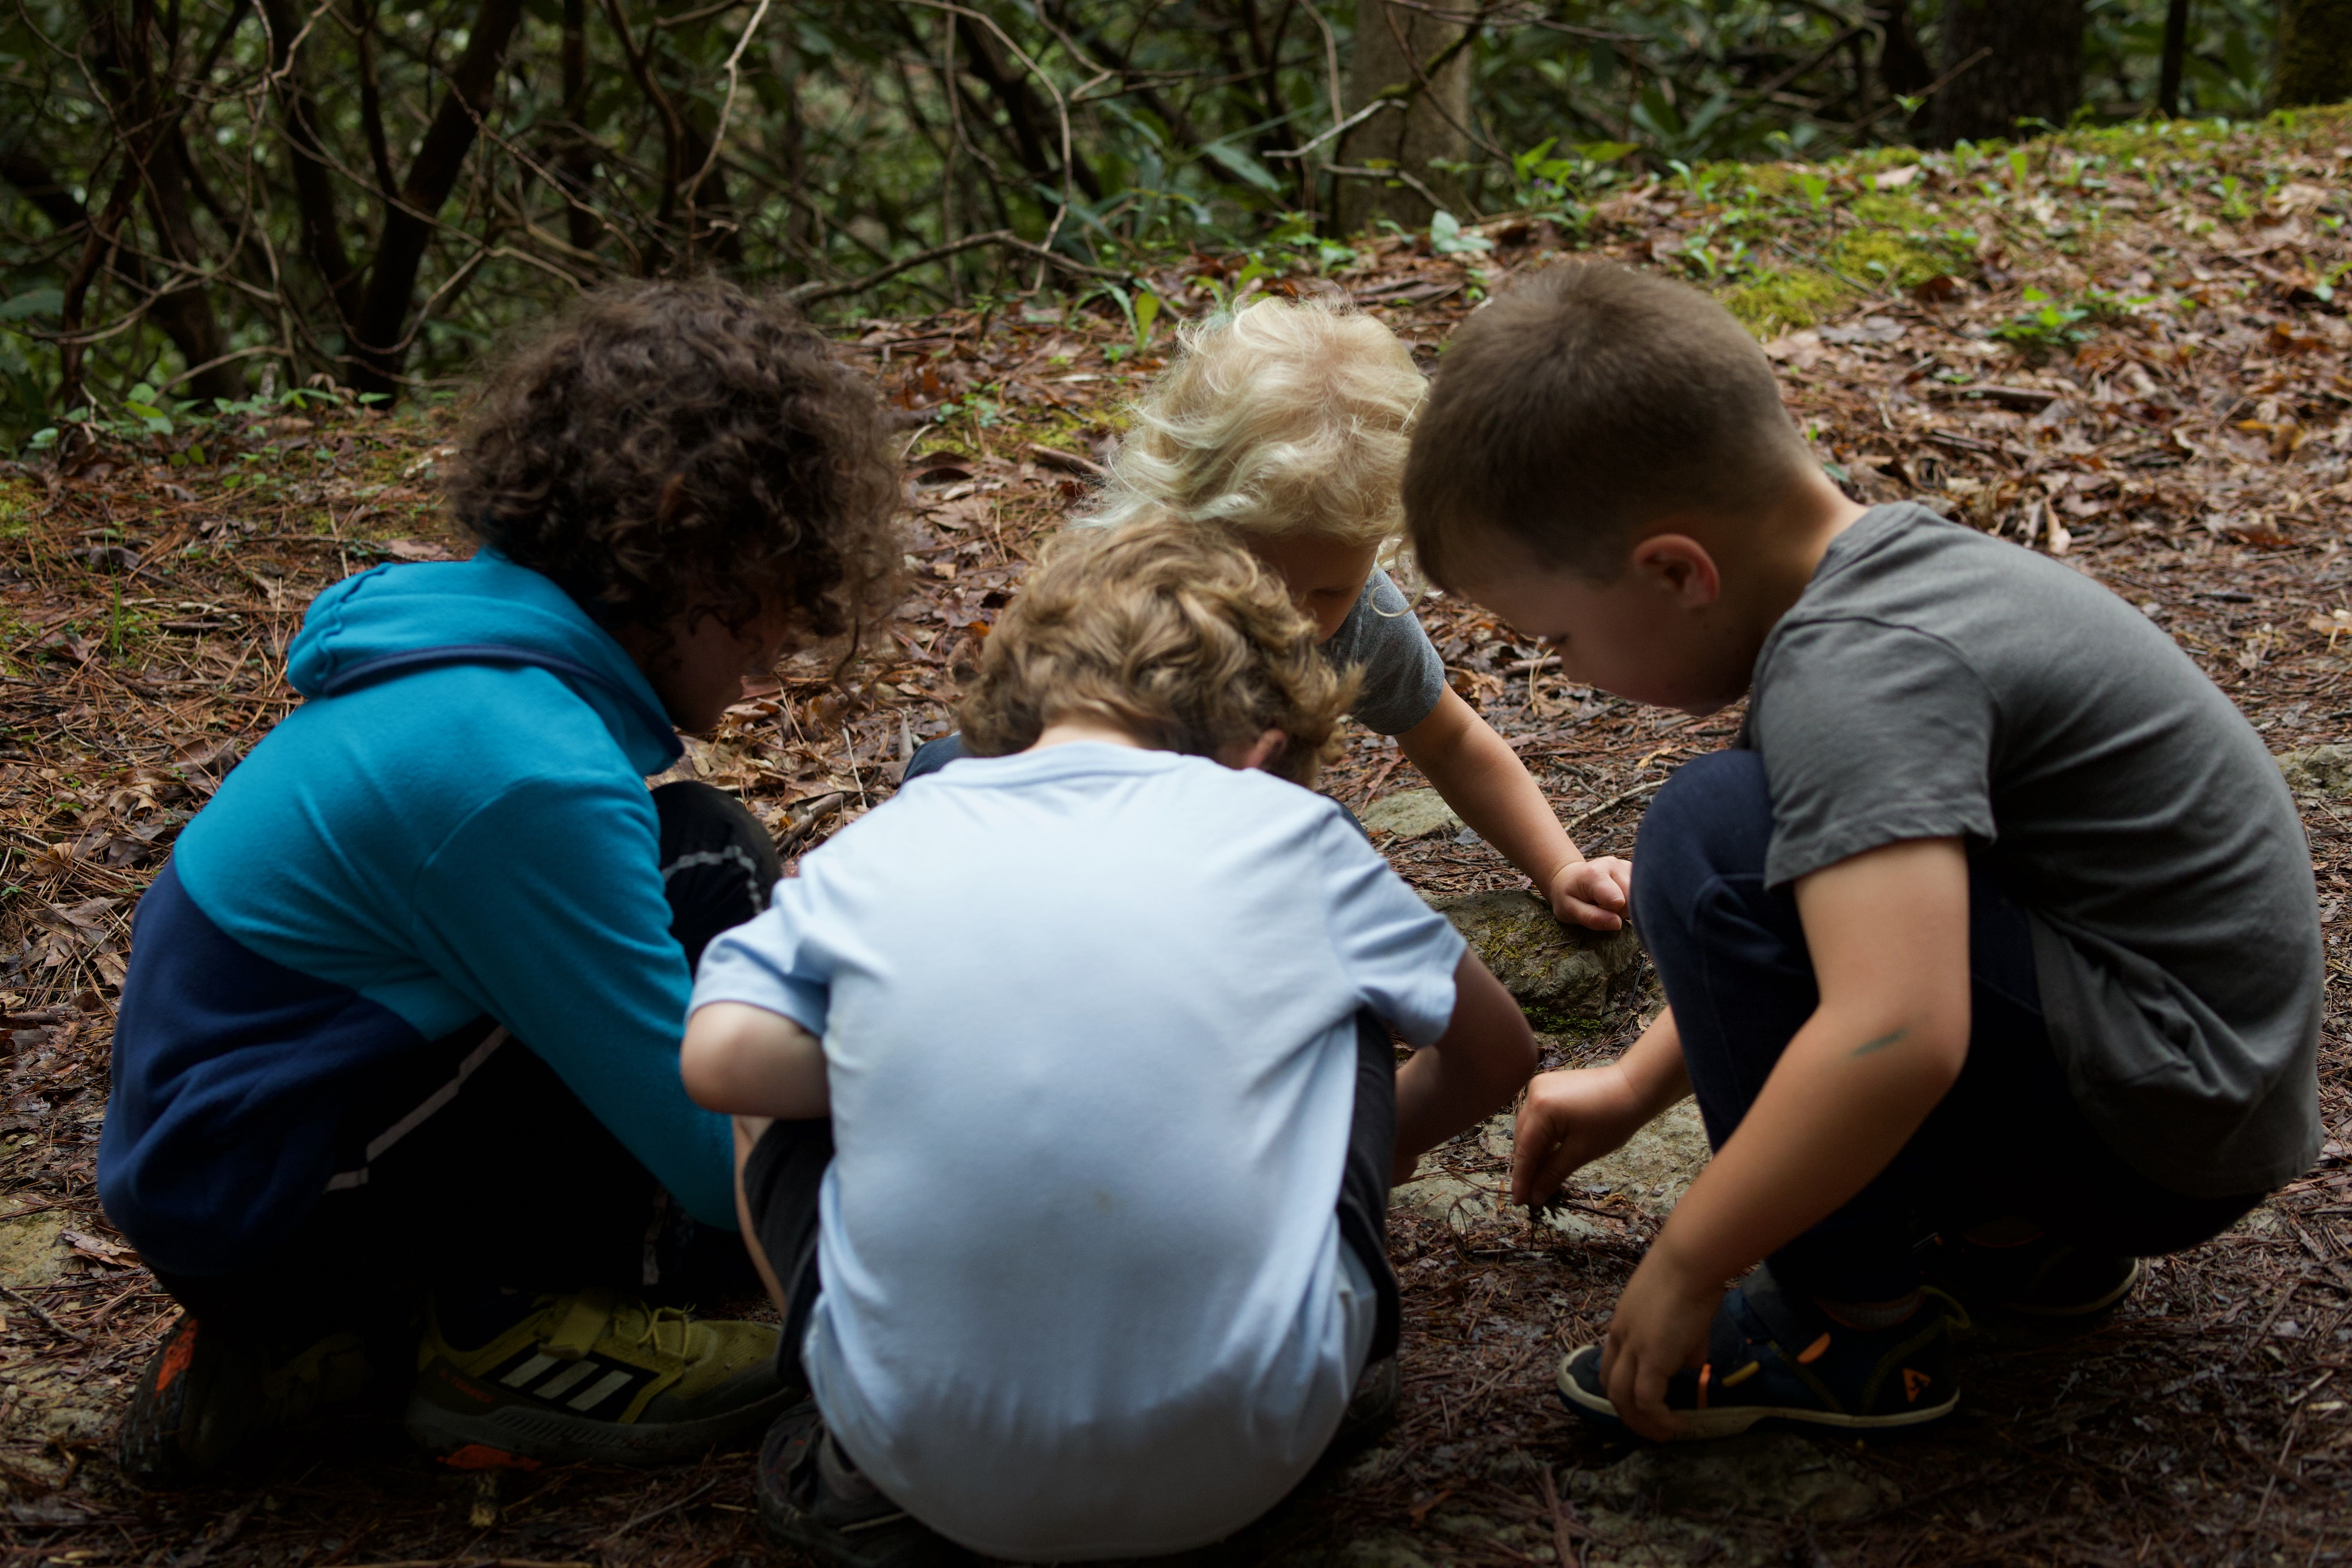
\includegraphics[keepaspectratio]{img/kidslooking.jpg}}

}

\caption{Photo credit to Katie and Joshua Rosenberg}

\end{figure}%

\subsection{Be choosy about the when and
where}\label{be-choosy-about-the-when-and-where}

One of the benefits of living close to great hiking opportunities is
that we can be a little choosy about when and where we hike. While we
are card carrying members of the puddle splashing club, we also
appreciate that our littles may have a better time when it is not 50°F
and rainy. Does it look like it is going to rain all day, border on
being too cold, or be oppressively hot? You can choose another day to
hike; we have enough good weather that we can avoid the less-than-ideal
days.

\begin{figure}[H]

{\centering \pandocbounded{\includegraphics[keepaspectratio]{img/trees-with-light.jpeg}}

}

\caption{Photo credit to Katie and Joshua Rosenberg}

\end{figure}%

\subsection{Plan for the essentials}\label{plan-for-the-essentials}

At a minimum, the following items are essential for hikes when the
weather is good and you are close to home:

\begin{itemize}
\tightlist
\item
  Water
\item
  Snacks
\item
  A waist pack or backpack
\end{itemize}

Older kids may like to carry some of these---especially the snacks!

\begin{figure}[H]

{\centering \pandocbounded{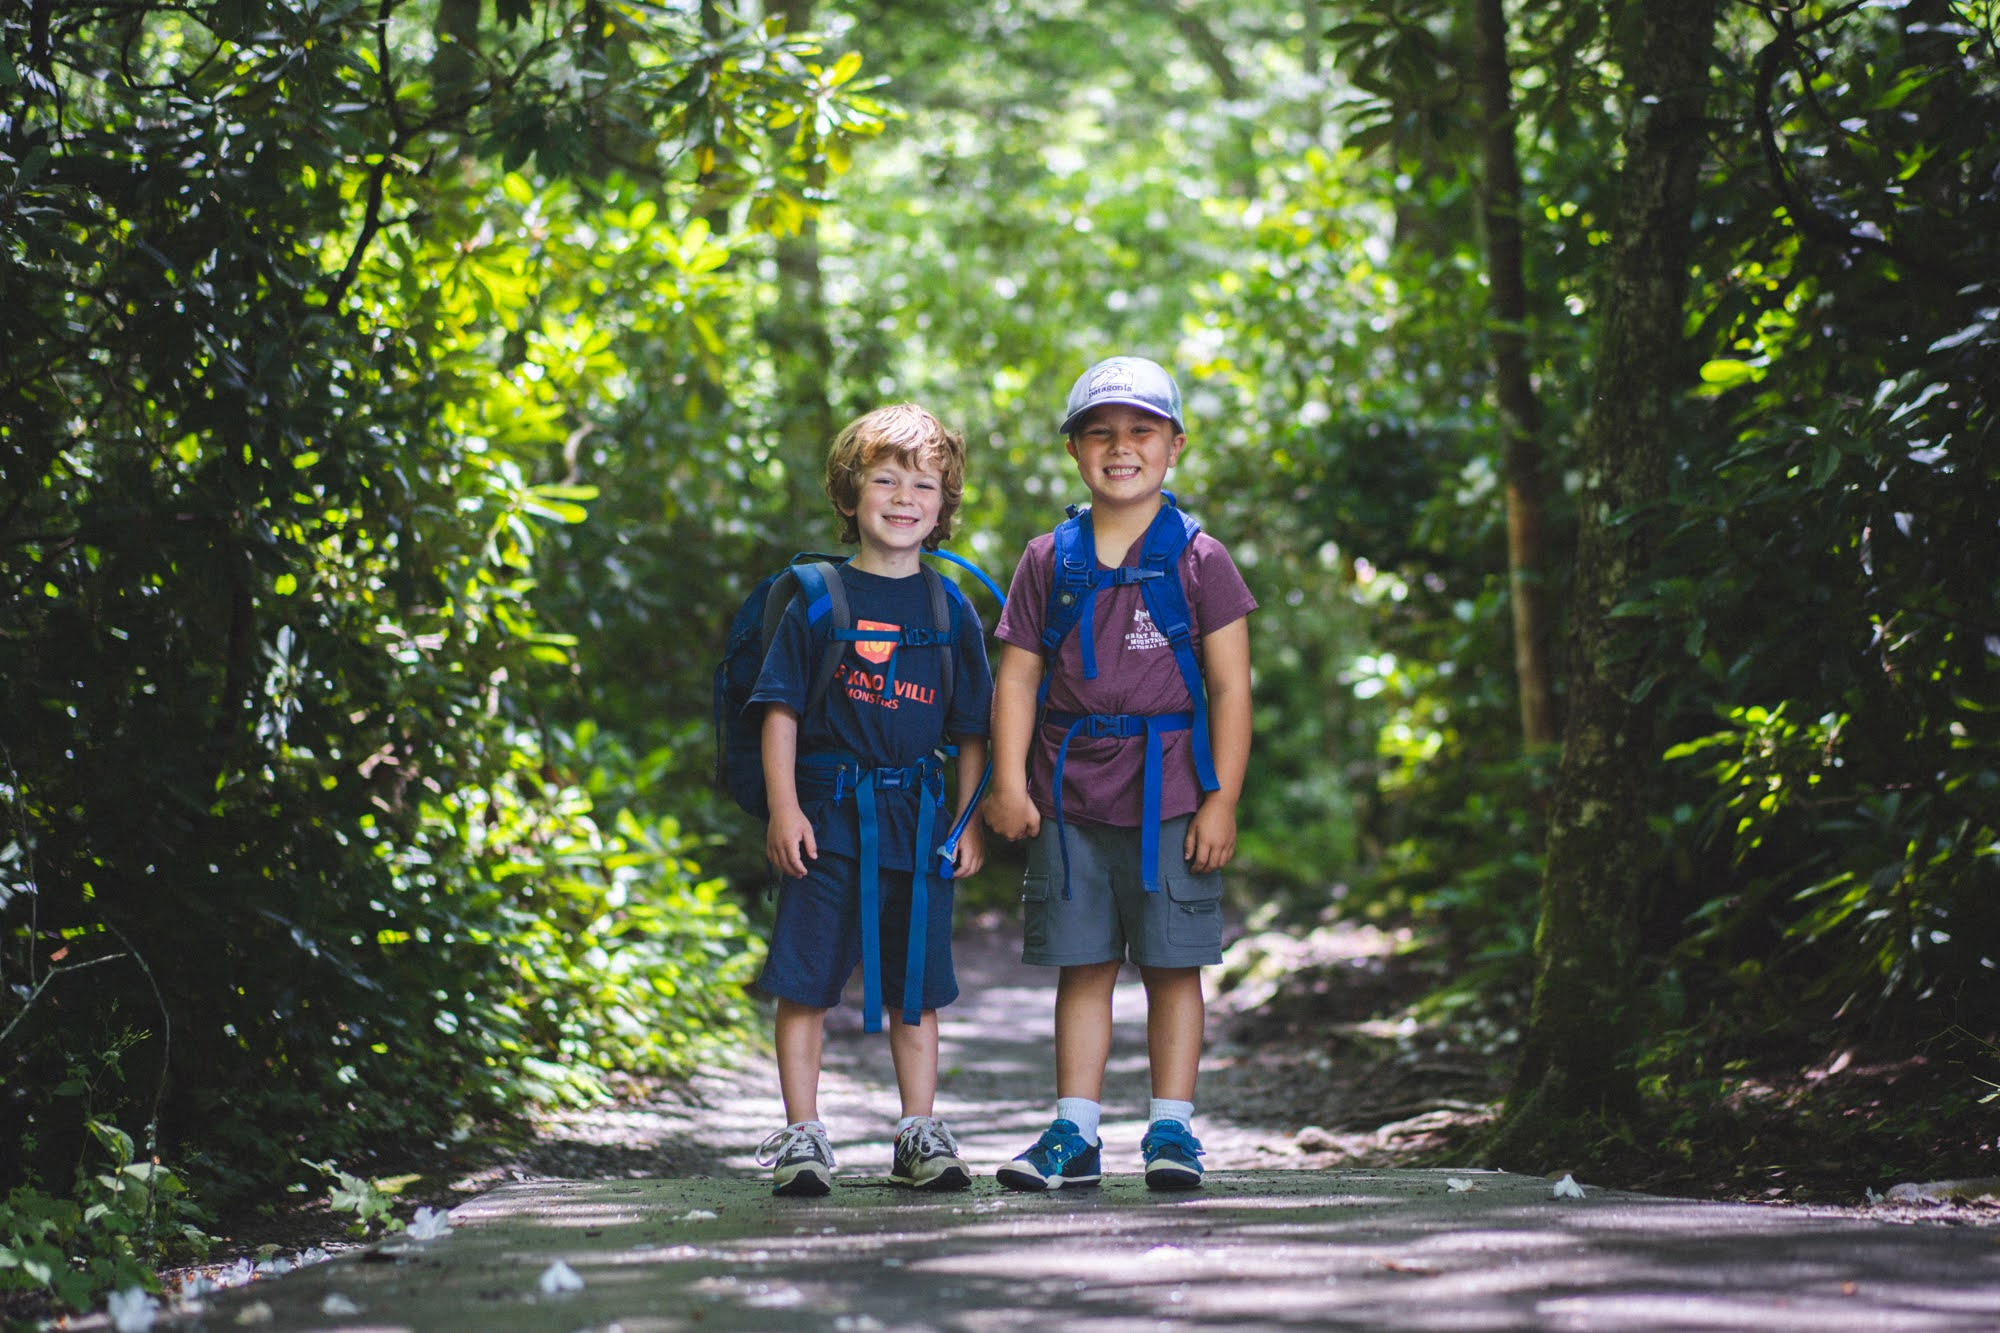
\includegraphics[keepaspectratio]{img/jo levi backpack.jpg}}

}

\caption{Photo credit to Sam Weisbrod}

\end{figure}%

When taking on a lengthier hike or traveling farther from home, we like
asking ourselves the following questions:

\textbf{What has the weather been?} \emph{What is the weather forecast?}
\emph{Is it bug season?}

These can help you to pack appropriately.

The appendix has some recommendations for a basic first-aid kit as well
as recommendations for some optional items you may wish to bring.

\subsection{Embrace serendipity}\label{embrace-serendipity}

It's good to have a plan, but don't be surprised if something better
comes along! Maybe you hike further than you thought you would, or
perhaps your child surprises you (and themselves!) by taking some time
to rock hop across a creek, follow animal tracks, or look at plants and
flowers. Be ready to follow your child's lead---whether that means
stopping to watch a butterfly or counting animal tracks. These moments
often become the most cherished.

\subsection{Select advice}\label{select-advice}

We asked some local hiking experts to share some additional advice.
Here's what they said:

\begin{itemize}
\tightlist
\item
  ``Kids need to find things they love on hiking.'' - Finn (3)
\item
  ``Find rocks while hiking.'' - Ruth (5)
\item
  ``When possible, swim in the waterfalls.'' - Ruth (5)
\item
  ``It's important to go off the trail.'' - Ruth (5)
\item
  ``If your baby can walk a little bit, then let them walk.'' - Jonah
  (age 6)
\item
  ``Make sure to run and also look for bears.'' - Levi (7)
\item
  ``You might want to bring pants and a sweatshirt with a hood. Because
  that one time I brought no pants and a sweatshirt with no hood.'' -
  G.H. (9)
\item
  ``Games and stories are better when made up on the fly.'' - D. (9)
\end{itemize}

The next chapter offers some guidance on how to pick a trail (and how to
use this book).

\part{Choosing a Hike}

\chapter{Overview of the Hikes}\label{overview-of-the-hikes}

\begin{longtable}[]{@{}
  >{\raggedright\arraybackslash}p{(\linewidth - 18\tabcolsep) * \real{0.0769}}
  >{\raggedright\arraybackslash}p{(\linewidth - 18\tabcolsep) * \real{0.1026}}
  >{\raggedright\arraybackslash}p{(\linewidth - 18\tabcolsep) * \real{0.1026}}
  >{\raggedright\arraybackslash}p{(\linewidth - 18\tabcolsep) * \real{0.1026}}
  >{\raggedright\arraybackslash}p{(\linewidth - 18\tabcolsep) * \real{0.1026}}
  >{\raggedright\arraybackslash}p{(\linewidth - 18\tabcolsep) * \real{0.1026}}
  >{\raggedright\arraybackslash}p{(\linewidth - 18\tabcolsep) * \real{0.1026}}
  >{\raggedright\arraybackslash}p{(\linewidth - 18\tabcolsep) * \real{0.1026}}
  >{\raggedright\arraybackslash}p{(\linewidth - 18\tabcolsep) * \real{0.1026}}
  >{\raggedright\arraybackslash}p{(\linewidth - 18\tabcolsep) * \real{0.1026}}@{}}
\toprule\noalign{}
\begin{minipage}[b]{\linewidth}\raggedright
Trail \#
\end{minipage} & \begin{minipage}[b]{\linewidth}\raggedright
\textbf{Trail Name}
\end{minipage} & \begin{minipage}[b]{\linewidth}\raggedright
\textbf{Time}
\end{minipage} & \begin{minipage}[b]{\linewidth}\raggedright
\textbf{Distance (Mi.)}
\end{minipage} & \begin{minipage}[b]{\linewidth}\raggedright
\textbf{Elevation}
\end{minipage} & \begin{minipage}[b]{\linewidth}\raggedright
\textbf{Pets}
\end{minipage} & \begin{minipage}[b]{\linewidth}\raggedright
\textbf{Parking Pass}
\end{minipage} & \begin{minipage}[b]{\linewidth}\raggedright
\textbf{Restrooms}
\end{minipage} & \begin{minipage}[b]{\linewidth}\raggedright
\textbf{Best Ages}
\end{minipage} & \begin{minipage}[b]{\linewidth}\raggedright
\textbf{Accessibility}
\end{minipage} \\
\midrule\noalign{}
\endhead
\bottomrule\noalign{}
\endlastfoot
1 & \textbf{Seven Islands} & 1.5 - 3 hours & 2.3 & Gentle & Allowed on
leash & Not Required & Yes & Toddlers, Little kids, and Big kids &
Partially accessible (path is paved until the island portion) \\
2 & \textbf{Ijams Riverside} & 45 minutes - 1.5 hours & 1.03 & Moderate
& Allowed on leash & Required (pay on site) & Yes & Toddlers and Little
Kids & Not accessible \\
3 & \textbf{Lakeshore Park} & 1.5 hours - 2.5 hours & 2.2 & Gentle &
Allowed on leash & Not Required & Yes & Toddlers, Little Kids, and Big
Kids & Not accessible \\
4 & \textbf{High Ground Park} & 0.5 hours - 1 hour & 0.7 & Gentle &
Allowed on leash & Not Required & No & Toddlers and Little kids &
Accessible \\
5 & \textbf{UT Arboretum} & 0.5 hours - 1 hour & 0.9 & Gentle & Not
Allowed & Not Required & No & Toddlers and Little Kids & Accessible \\
6 & \textbf{Knox-Blount Greenway} & 45 minutes - 1.5 hours & 2.3 &
Gentle & Allowed on leash & Not Required & No & Toddlers and Little Kids
& Accessible \\
7 & \textbf{Sequoyah Park} & 1 hour - 2 hours & 2.1 & Flat & Allowed on
leash & Not Required & Yes & Toddlers and Little Kids & Not
accessible \\
8 & \textbf{Ijams Crag} & 45 minutes - 1.5 hours & 1.5 & Moderate &
Allowed on leash & Not Required & Yes & Little Kids and Big Kids & Not
accessible \\
9 & \textbf{William Hastie} & 0.5 hours - 1 hour & 1.3 & Flat & Allowed
on leash & Not Required & No & Toddler and little kids & Partially
accessible (graded gravel path) \\
10 & \textbf{Sharp's Ridge} & 1.5 hours - 2.5 hours & 2.3 & Moderate &
Allowed on leash & Not Required & No & Little kids & Not accessible \\
11 & \textbf{Norris Dam} & 1.5 hours - 2.5 hours & 2.3 & Gentle &
Allowed on leash & Not Required & No & Little kids and Big kids &
Partially accessible (graded gravel path) \\
12 & \textbf{House Mountain} & 2.5 hours - 4.5 hours & 2.5 & Steep &
Allowed on leash & Not Required & No & Pre-teens and older & Not
accessible \\
13 & \textbf{Emory Falls at Frozen Head} & 2 hours - 3.5 hours & 2.4 &
Moderate & Allowed on leash & Not Required & No & Little kids & Not
accessible \\
14 & \textbf{The Obed Point Trail} & 2.5 hours - 4.5 hours & 3.6 &
Gentle & Allowed on leash & Not Required & Yes & Little kids and Big
kids & Not accessible \\
15 & \textbf{Bandy Creek Campground} & 45 minutes - 1.25 hours & 1.3 &
Flat & Allowed on leash & Not Required & Yes & Toddlers and Little kids
& Not accessible \\
16 & \textbf{Fall Branch Falls} & 2.5 hours - 4.5 hours & 3.7 & Moderate
& Allowed on leash & Not Required & Yes & Big kids and Pre-teens and
older & Not accessible \\
17 & \textbf{Twin Arches} & 1.5 hour - 2.5 hours & 1.2 & Moderate &
Allowed on leash & Not Required & Yes & Little kids and Big kids & Not
accessible \\
18 & \textbf{Angel Falls Overlook} & 1.5 hours - 2.5 hours & 2.8 &
Gentle & Allowed on leash & Not Required & No & Little Kids and Big Kids
& Not Accessible \\
19 & \textbf{Honey Creek} & 4 hours - 7 hours & 4.4 & Steep & Not
Allowed & Required & No & Big kids and Pre-teens and older & Not
accessible \\
20 & \textbf{Spruce Flats Falls} & 1.5 hours - 2.5 hours & 1.6 &
Moderate & Not Allowed & Required & Yes & Big kids and Pre-teens and
older & Not accessible \\
21 & \textbf{Little River} & 3 hours - 5 hours & 5.5 & Moderate & Not
Allowed & Required & No & Little kids, Big kids, and Pre-teens and older
& Not accessible \\
22 & \textbf{Mouse Creek} & 2 hours - 4 hours & 4.0 & Moderate & Not
Allowed & Required & Yes (seasonal) & Little kids and Big kids & Not
accessible \\
23 & \textbf{Whiteoak Sink} & 3 hours - 5 hours & 4.6 & Moderate & Not
Allowed & Required & No & Little kids and Big kids & Not accessible \\
24 & \textbf{Middle Prong} & 4 hours - 6 hours & 7.6 & Moderate & Not
Allowed & Required & No & All Ages & Not accessible \\
25 & \textbf{Abrams Creek} & 4 hours - 6 hours & 5.8 & Moderate & Not
Allowed & Required & Yes (seasonal) & All ages & Not accessible \\
26 & \textbf{Look Rock} & 30 minutes - 1 hour & 0.6 & Moderate & Not
Allowed & Required & No & Toddlers and Little Kids & Partially
accessible (paved but very steep) \\
27 & \textbf{Chestnut Top} & 1.5 hours - 2.5 hours & 2.6 & Steep & Not
Allowed & Required & No & Big kids & Not accessible \\
28 & \textbf{Abrams Falls} & 3 hours - 2.5 hours & 5.0 & Steep & Not
Allowed & Required & Yes & Big kids and Pre-teens and older & Not
accessible \\
29 & \textbf{Andrews Bald} & 2 hours - 3.5 hours & 3.6 & Moderate & Not
Allowed & Required & Yes (seasonal) & Big kids and Pre-teens and older &
Not accessible \\
30 & \textbf{Alum Cave Bluffs} & 3 hours - 5 hours & 4.5 & Very Steep &
Not Allowed & Required & Yes (seasonal) & Big kids and Pre-teens and
older & Not accessible \\
\end{longtable}

\chapter{What Each Chapter Includes}\label{what-each-chapter-includes}

\subsection{Overview}\label{overview}

Each of the chapters for hikes starts with an \emph{Overview} that give
a sense for ``look and feel'' of the hike.

\subsection{Key Characteristics}\label{key-characteristics}

After each overview is a table with \emph{Key Characteristics} of the
trail, including for which ages of children the hike is best.

\begin{itemize}
\tightlist
\item
  \emph{Toddlers}: One-two year-olds who can walk some of the trail
  (being carried for other parts) or all of short trails.
\item
  \emph{Little kids}: Two- four or five years who can walk all of short
  trails and even some parts of lengthier trails.
\item
  \emph{Big kids}: Four -eight or nine who can walk longer distances and
  who are up for bigger challenges
\item
  \emph{Pre-teens and older}: Eight or nine and up
\end{itemize}

Of course, you may also choose to carry your toddler, little kid, or
younger big kid for some or all of these hikes.

The key characteristics also include the length of the hike,
approximately how long it takes to hike, the elevation change (Flat,
Gentle, Moderate, Steep, and Very Steep), whether pets are allowed a
parking pass required, and the presence of a restroom. Finally, we also
note whether the trail is accessible for those with strollers and
wheelchairs.

\subsection{Trail Maps and Photos}\label{trail-maps-and-photos}

Each hike has a \textbf{trail maps}. These should be pretty
straightforward to use. Trailheads---the starting points for the
hikes---are marked with a green dot, and the trail is in red, with key
features of the trail noted along the way. We also include one or more
photos for each hike; we tried to select these to show what makes the
hike unique.

\subsection{Call outs}\label{call-outs}

The hikes are through areas rich in natural and human history, and while
we felt comfortable accurately describing many of these elements, we
felt we had to enlist the help of friends and colleagues for
others---for which we have \textbf{``call outs''}. Look for these in the
call-outs in most of the chapters, and consider sharing parts of them
with your little hikers.

\subsection{Doing more}\label{doing-more}

Each chapter concludes with one or more things to do nearby, from places
to grab a bite to eat to other, nearby hikes to consider.

\chapter{Finding a Hike}\label{finding-a-hike}

Lists of \emph{the best} hikes are helpful, but they can lead you to
trails that are far away, crowded, and not suited to young kids.
Furthermore, what even is \emph{the best} trail to kids?

We bet you've had the experience on a family trip to someplace special
only for your kiddo to be captivated by the stairs near the
entrance---or, you bought a pricey gift only for the cardboard box to be
the best part.

There's something similar when it comes to finding a hike: Which hike is
the best can be really hard to predict in advance!

Still, we think you can set yourself up for success: We picked the hikes
that are in the sweet spot for parents of younger children: not too far
away, not so challenging as to be discouraging to kids and their
parents; near amenities; and scenic and rewarding to accomplish.

\subsection{Choosing where to hike}\label{choosing-where-to-hike}

Some trails are short, flat, and on a paved surface. Others are longer,
steeper, or rockier. How do you find which one is best for you?

\begin{figure}[H]

{\centering \pandocbounded{\includegraphics[keepaspectratio]{img/rocky trail.jpg}}

}

\caption{Photo credit to Katie and Joshua Rosenberg}

\end{figure}%

This book has three sections, one each for hikes in and around
Knoxville, on the Cumberland Plateau, and in the Great Smoky Mountains
National Park. Within each section, we organized each hike loosely along
the lines of those we'd recommend first.

Thus, the first few hikes in each section are what we think of as ``sure
bets.'' Get the weather right, pack a bunch of snacks, and we think
you'll likely have a good time. We also created a list of Top 5 Hikes
that can help with choosing where to hike first.

For example, Seven Islands in Knoxville is a reliable choice, with paved
paths, beautiful views, and plenty of spots for kids to explore. Indeed,
if you haven't hiked there yet and the weather is good, we recommend you
stop reading now and head out!

Each chapter has a lot of information you can use to choose your
hike---particularly information in the \textbf{Overview} and \textbf{Key
Characteristics} sections. You can those for inspiration. All of the key
characteristics are also provided in a table in the Overview section for
easy review.

Last, the next chapter includes a list of ``Top 5s'' - our top
recommendations for hikes with different characteristics. Check those
out and pick a hike, and you're ready to head out!

\chapter{Top 5 Hikes}\label{top-5-hikes}

Here are some hikes that we recommend for different reasons--and ages of
kids.

\subsection{For Hiking With Babies and
Infants}\label{for-hiking-with-babies-and-infants}

\emph{These hikes are great when a short distance and a paved path are a
priority.}

\begin{enumerate}
\def\labelenumi{\arabic{enumi}.}
\tightlist
\item
  High Ground Park
\item
  Knox-Blount Greenway
\item
  Lakeshore Park
\item
  UT Arboretum
\item
  Norris Dam
\end{enumerate}

\subsection{Real Hikes for Little Explorers Walking on Their
Own}\label{real-hikes-for-little-explorers-walking-on-their-own}

\emph{These are ``real'' hikes--you and your little will know it!--but
they're also a reasonable distance and with not-too-challenging
terrain.}

\begin{enumerate}
\def\labelenumi{\arabic{enumi}.}
\tightlist
\item
  Ijams Riverside
\item
  Seven Islands
\item
  Emory Falls
\item
  Abrams Creek
\item
  Chestnut Tops
\end{enumerate}

\subsection{For Kids Who Need a Playground
Nearby}\label{for-kids-who-need-a-playground-nearby}

\emph{Who doesn't love a hike that starts and ends at or near a
playground?}

\begin{enumerate}
\def\labelenumi{\arabic{enumi}.}
\tightlist
\item
  Lakeshore
\item
  Emory Fall
\item
  Ijams Riverside
\item
  Ijams Crag
\item
  Sequoyah Park
\end{enumerate}

\subsection{For Kids Who Love to Play in the
Water}\label{for-kids-who-love-to-play-in-the-water}

\emph{These hikes are great in warmer weather; bring the right clothing
and shoes and let 'em splash!}

\begin{enumerate}
\def\labelenumi{\arabic{enumi}.}
\tightlist
\item
  Middle Prong
\item
  Abrams Creek
\item
  Spruce Flats Falls
\item
  Honey Creek
\item
  Mouse Creek
\end{enumerate}

\subsection{Best Spots for a Picnic}\label{best-spots-for-a-picnic}

\emph{Each of these is a fantastic place to have a family picnic.}

\begin{enumerate}
\def\labelenumi{\arabic{enumi}.}
\tightlist
\item
  Mouse Creek
\item
  Lakeshore
\item
  Seven Islands
\item
  Sequoyah Park
\item
  Ijams Crag
\end{enumerate}

\subsection{Bigger Adventures for Bigger
Kids}\label{bigger-adventures-for-bigger-kids}

*More challenging hikes for kids who are ready for the next challenge;
completing any of these is an achievement.

\begin{enumerate}
\def\labelenumi{\arabic{enumi}.}
\tightlist
\item
  Alum Cave -
\item
  Andrews Bald -
\item
  Honey Creek -
\item
  Little River
\item
  Abrams Falls
\end{enumerate}

\part{Knoxville and its Surroundings}

Knoxville and the Tennessee Valley contain fewer high points than the
Cumberland Plateau and the Great Smoky Mountains, but it should not be
discounted as a destination for hiking.

We think a trip to Seven Islands State Birding Park will make evident
how spectactular this area can be. Around 30 minutes away from most
places in Knoxville, this is a true destination not only for birders,
but also hikers and paddlers.

Other locations are also not only close, but (surprisingly) worthy of a
trip. Ijams on the south side of Knoxville--familiar to many in the
Knoxville area--has many spectacular features, in addition to being
fewer than ten minutes away from downtown.

Other places that we highlight among the 12 trails in this secton are
very worth your time, offering an outdoors respite in addition to the
ability to easily be integrated into busy schedules and other
commitments. If you are looking for a first family hike, those in this
section may make a great selection.

\pandocbounded{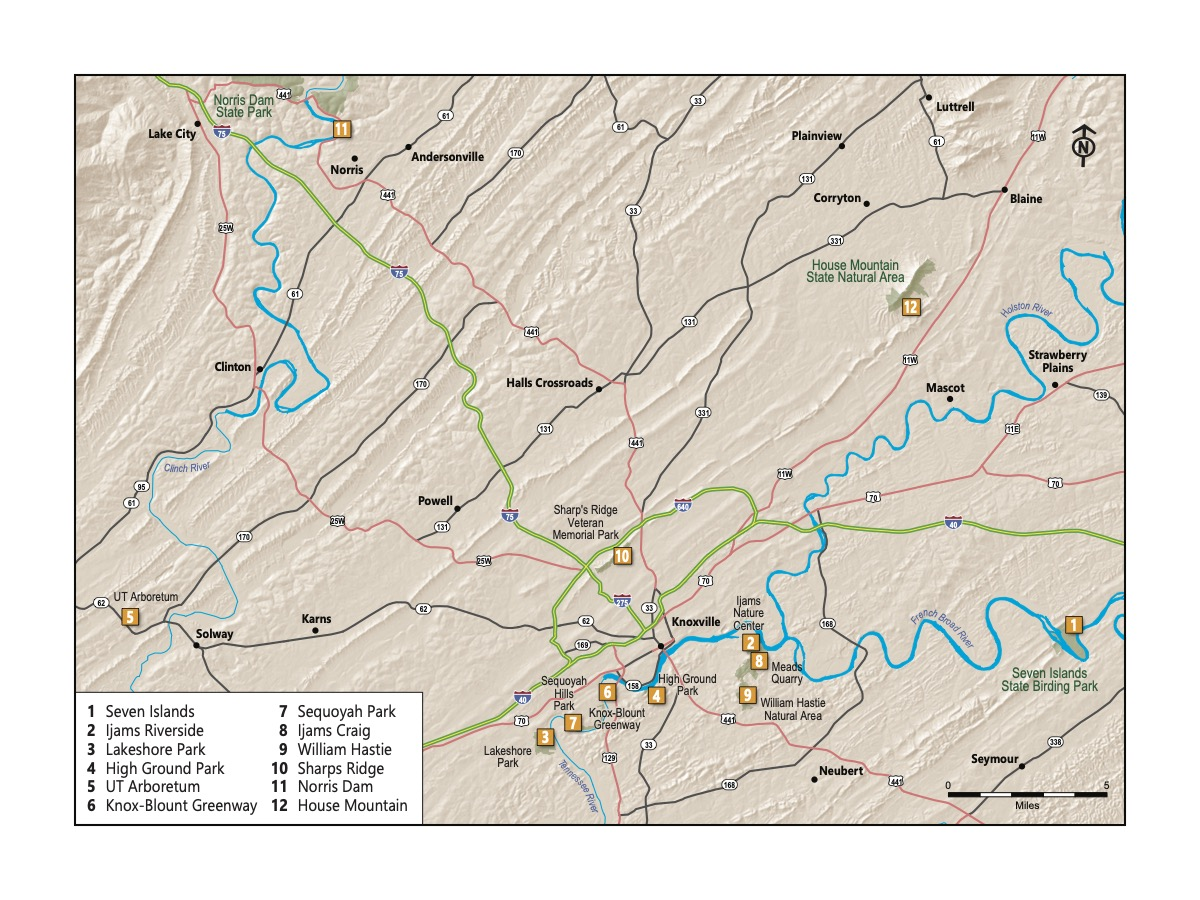
\includegraphics[keepaspectratio]{maps/knoxville-region.jpg}}

\chapter{Trail 1: Seven Islands}\label{trail-1-seven-islands}

\subsection{Overview}\label{overview-1}

This is one of our favorite trails in this book, and it is the first
trail for that reason! This hike is a crowd pleaser for every family
member of all ages thanks to a paved path that makes bringing babies in
a stroller a breeze and easy acces to experience meadow, woodland, and a
river! For the trail we highlight, a paved path descends through a
meadow. Look for varied bird varieties and deer in all seasons! The
trail crosses a bridge over the French Broad River and then a dirt trail
make a loop around a beautiful island before returning back to the paved
path. This hike is great for all ages and seasons, though it is
sometimes hot in the summer due to limited shade on the paved part of
the trail.

\begin{figure}[H]

{\centering \pandocbounded{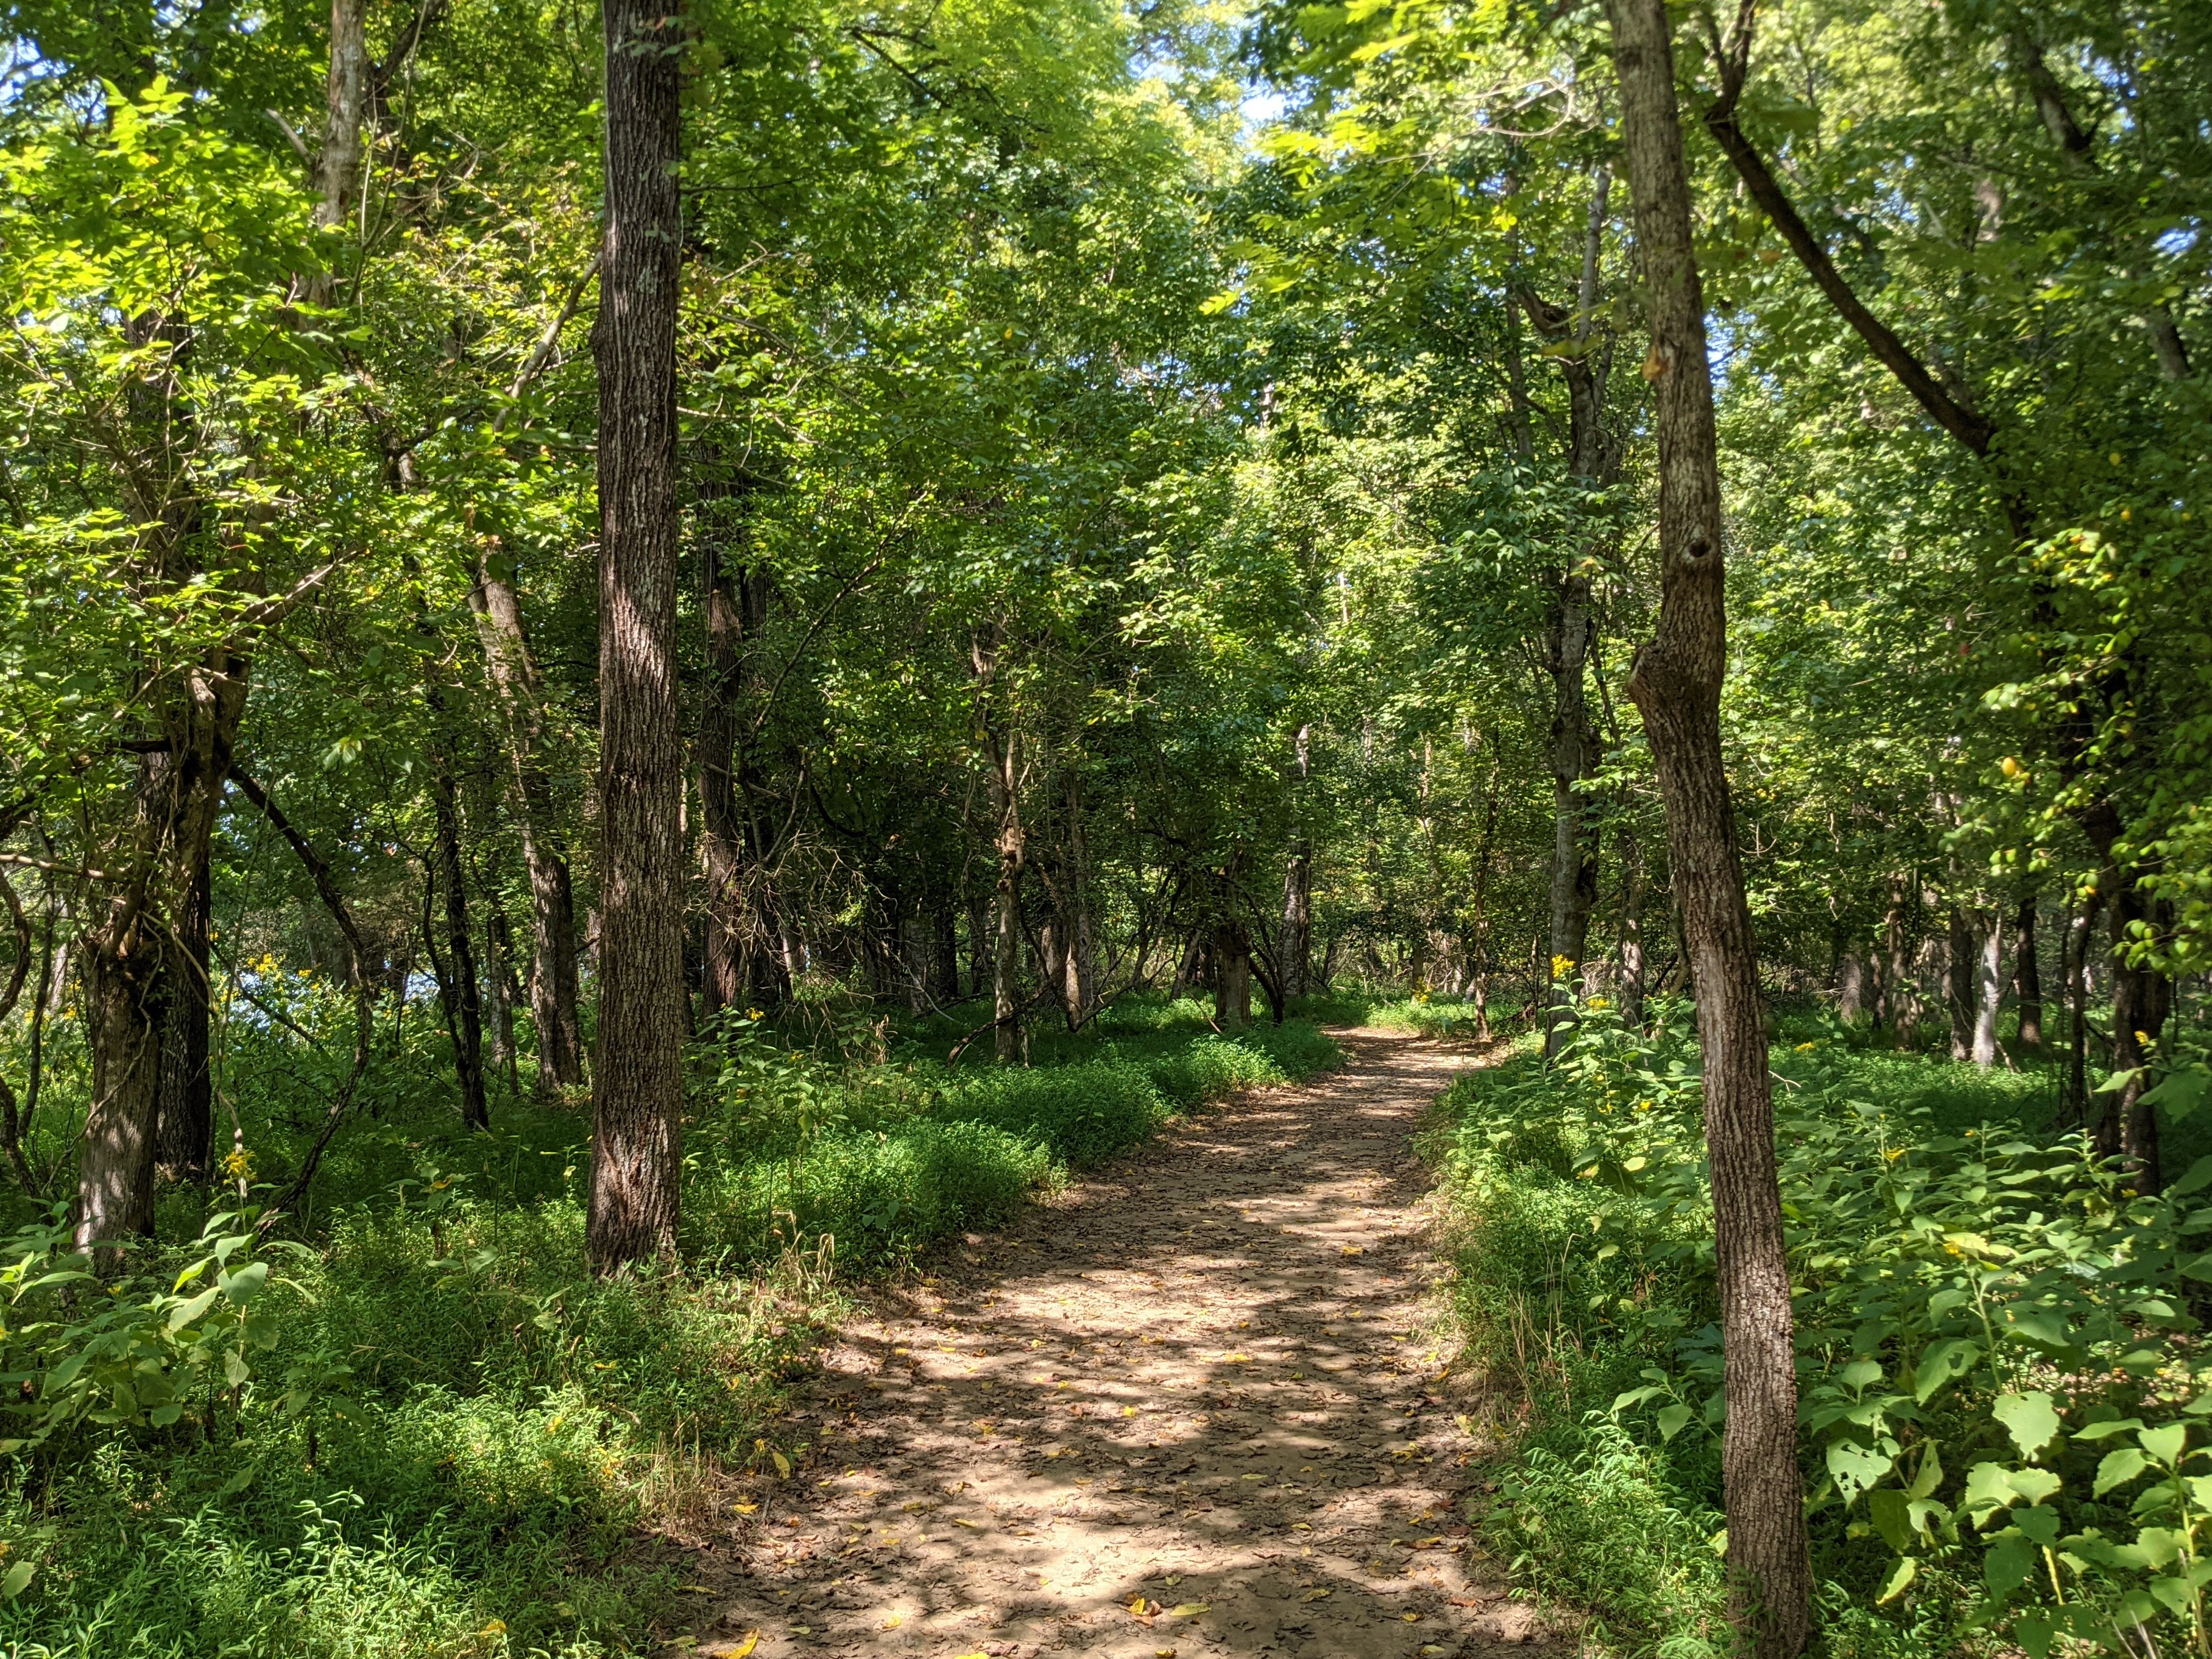
\includegraphics[keepaspectratio]{img/trail-01-figure-01.jpg}}

}

\caption{Photo credit to Katie and Joshua Rosenberg}

\end{figure}%

\subsection{Key Characteristics}\label{key-characteristics-1}

\begin{longtable}[]{@{}
  >{\raggedright\arraybackslash}p{(\linewidth - 2\tabcolsep) * \real{0.6170}}
  >{\raggedright\arraybackslash}p{(\linewidth - 2\tabcolsep) * \real{0.3830}}@{}}
\toprule\noalign{}
\begin{minipage}[b]{\linewidth}\raggedright
\textbf{Characteristic}
\end{minipage} & \begin{minipage}[b]{\linewidth}\raggedright
\textbf{Details}
\end{minipage} \\
\midrule\noalign{}
\endhead
\bottomrule\noalign{}
\endlastfoot
Time Estimate - Hiking Fast & 1.5 - 3 hours \\
Trail Distance (Miles) & 2.3 \\
Elevation Change & Gentle \\
Pets & Allowed on leash \\
Parking Pass/Entrance Fee & Not Required \\
Restroom(s) & Yes \\
Best Ages & Toddlers, Little kids, and Big kids \\
Strollers and Wheelchairs & Partially accessible (path is paved until
the island portion) \\
\end{longtable}

\pandocbounded{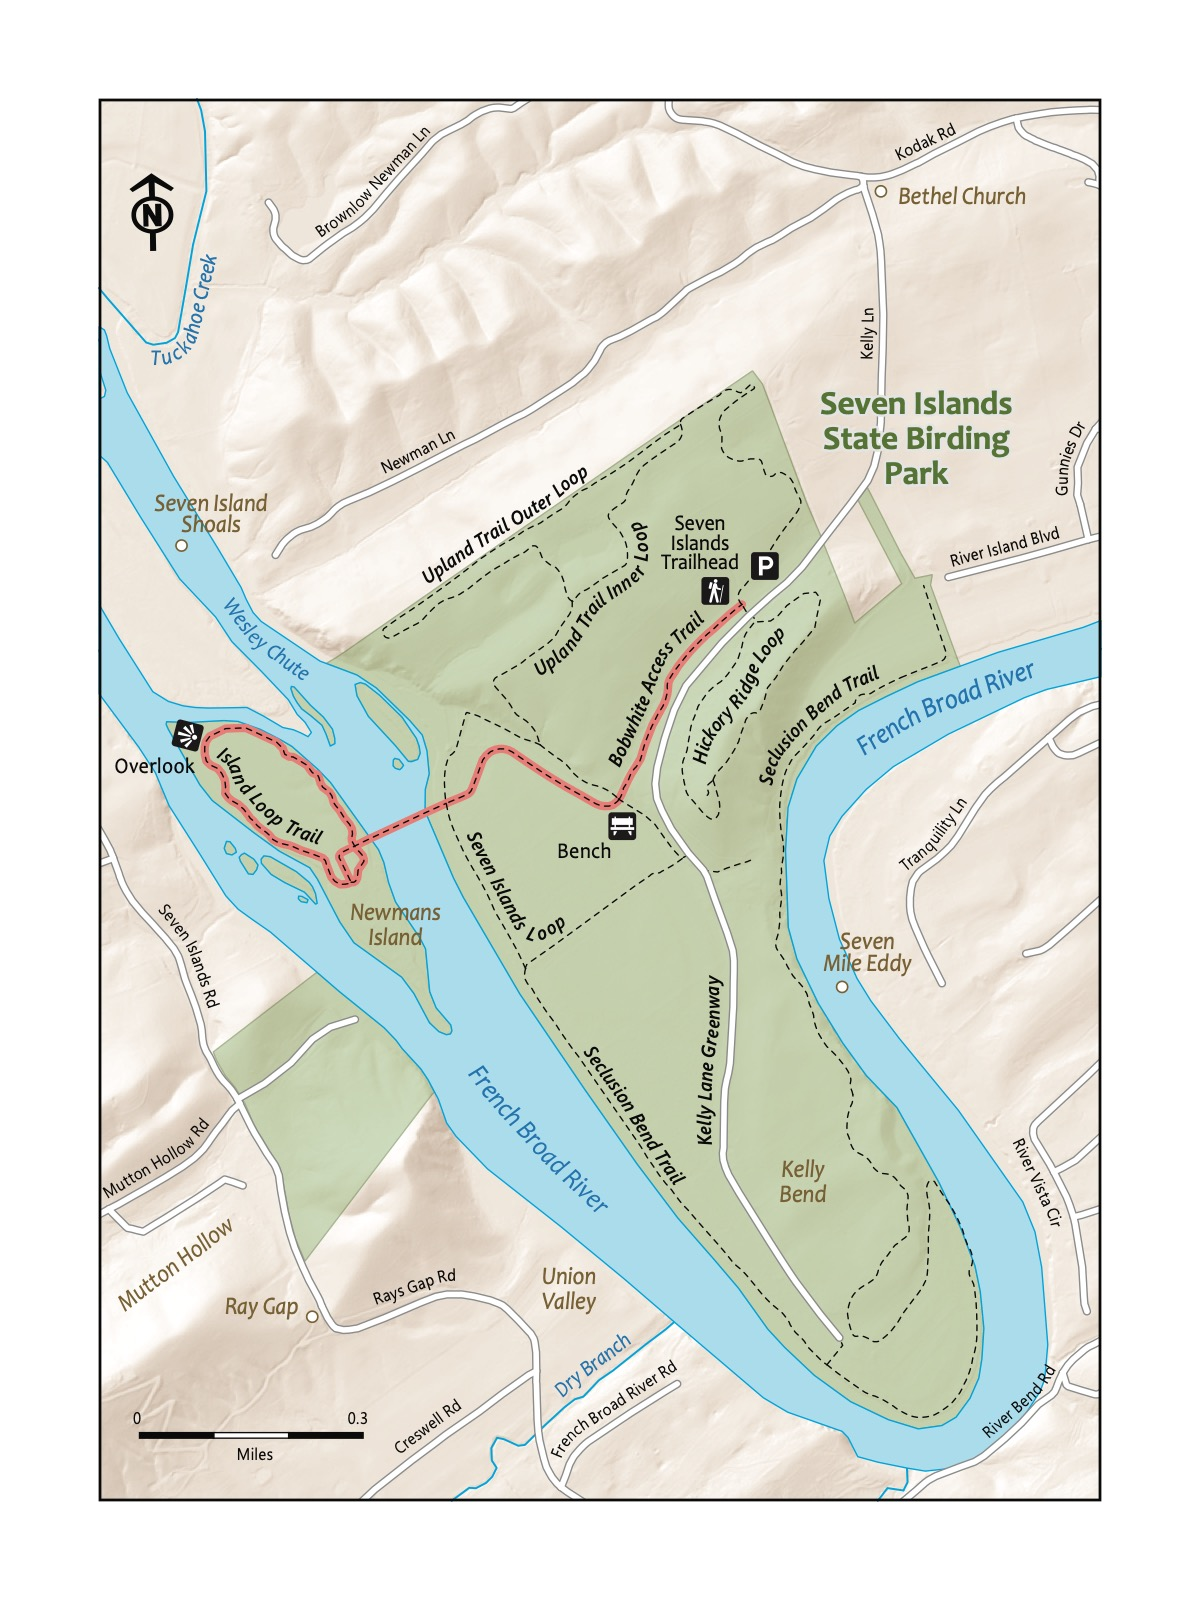
\includegraphics[keepaspectratio]{maps/trail-01-map.jpeg}}

\subsection{Directions to the
Trailhead}\label{directions-to-the-trailhead}

Trailhead Address: Seven Islands State Birding Park, 2809 Kelly Ln,
Kodak, TN 37764

Trailhead GPS Coordinates: 35.95366, -83.68701

Park in the large gravel lot (note there is another parking area by a
boat launch that is not the correct location for this hike!). We have
never had trouble finding a spot even on the busiest of days.

\begin{tcolorbox}[enhanced jigsaw, colback=white, colframe=quarto-callout-note-color-frame, breakable, opacityback=0, toprule=.15mm, bottomrule=.15mm, rightrule=.15mm, left=2mm, leftrule=.75mm, arc=.35mm]
\begin{minipage}[t]{5.5mm}
\textcolor{quarto-callout-note-color}{\faInfo}
\end{minipage}%
\begin{minipage}[t]{\textwidth - 5.5mm}

\vspace{-3mm}\textbf{Paw Paw}\vspace{3mm}

A native fruit found around Seven Islands. Tastes like a mix of an apple
and a banana. Paw Paw flowers are pollinated by beetles and flies.

\end{minipage}%
\end{tcolorbox}

\subsection{Trail Description}\label{trail-description}

\begin{longtable}[]{@{}
  >{\raggedright\arraybackslash}p{(\linewidth - 2\tabcolsep) * \real{0.2000}}
  >{\raggedright\arraybackslash}p{(\linewidth - 2\tabcolsep) * \real{0.8000}}@{}}
\toprule\noalign{}
\begin{minipage}[b]{\linewidth}\raggedright
Distance from Start
\end{minipage} & \begin{minipage}[b]{\linewidth}\raggedright
Description
\end{minipage} \\
\midrule\noalign{}
\endhead
\bottomrule\noalign{}
\endlastfoot
0.0 & Access the Bobwhite Access Trail by walking around or through the
barn. \\
0.05 & Bathroom on the left of the trail. \\
0.1 & Descend through grassy meadows with wildflowers in the spring and
early fall. \\
0.3 & Bench makes for a nice rest spot. \\
0.6 & Start of the Newmans Island Bridge. \\
0.8 & Paved trail ends. Turn right onto the Island Loop Trail to hike
around the island. \\
0.85 & Picnic table beside a pretty part of the French Broad River. \\
1.05 & Stick house (kiddo favorite!). \\
1.5 & Connect back to the bridge, heading back onto the Bobwhite Access
Trail. \\
2 & Climb back up the Bobwhite Access Trail to the trailhead. \\
2.3 & Trailhead. \\
\end{longtable}

\subsection{Nearby}\label{nearby}

\begin{tcolorbox}[enhanced jigsaw, colback=white, colframe=quarto-callout-note-color-frame, breakable, opacityback=0, toprule=.15mm, bottomrule=.15mm, rightrule=.15mm, left=2mm, leftrule=.75mm, arc=.35mm]
\begin{minipage}[t]{5.5mm}
\textcolor{quarto-callout-note-color}{\faInfo}
\end{minipage}%
\begin{minipage}[t]{\textwidth - 5.5mm}

\vspace{-3mm}\textbf{Eastern Bluebird}\vspace{3mm}

While many birds stop over at Seven Islands and areas like that on their
migratory routes south (in the fall) and north (in the spring), the
Eastern Bluebird is a year-round resident. Bluebirds are obligate cavity
nesters - which is why they have experienced such a decline in their
population as urban sprawl has increased. Refuges like Seven Islands
give them lots of opportunities to find natural cavities to nest in!
-MaryRose Weatherton

\end{minipage}%
\end{tcolorbox}

\begin{itemize}
\tightlist
\item
  \textbf{Take advantage of the other trails nearby!} Hike up the
  Hickory Ridge trail, another trail at Seven Islands State Birding
  Park, that is accessible from just behind the bathrooms near the
  parking lot. There are several other great hikes available, including
  hikes down the Kelly Lane Greenway (the other, wider, paved path near
  the barn that is gated to prevent cars from driving on it) and the
  Upland Inner and Outer Trail Loops.
\item
  \textbf{Bring your canoe, kayak, or paddle board for even more
  adventures!} Access parking by Also, River Sports Outfitters rents
  kayaks and canoes here during the summer (see
  \hyperref[0]{https://www.riversportsoutfitters.com/}).
\item
  \textbf{Stop for a bite to eat and a drink on the way back!} Consider
  stopping by kid-friendly Walnut Springs Winery (1175 Midway Rd,
  Knoxville, TN 37914), open Wednesday-Sunday as of this writing.
\end{itemize}

\chapter{Trail 2: Ijams Riverside}\label{trail-2-ijams-riverside}

\subsection{Overview}\label{overview-2}

It's easy to take this destination for granted if you live in Knoxville
-- we seem to find something new every time we visit! Bring along your
baby carrier for this hike, which is meant to be a gentle introduction
to what Ijams refers to as the Riverside area. The trail starts by the
Ijams Nature Center's visitor center and meanders down through a deep
forest to the river. It continues along the boardwalk trail that happens
to follow the side of the very first mile of the Tennessee River. The
trail returns back up and over a rocky ridge to return to the visitor
center. Ijams offers multiple play areas and links to other trails
nearby, so you can make a day of it!

\begin{figure}[H]

{\centering \pandocbounded{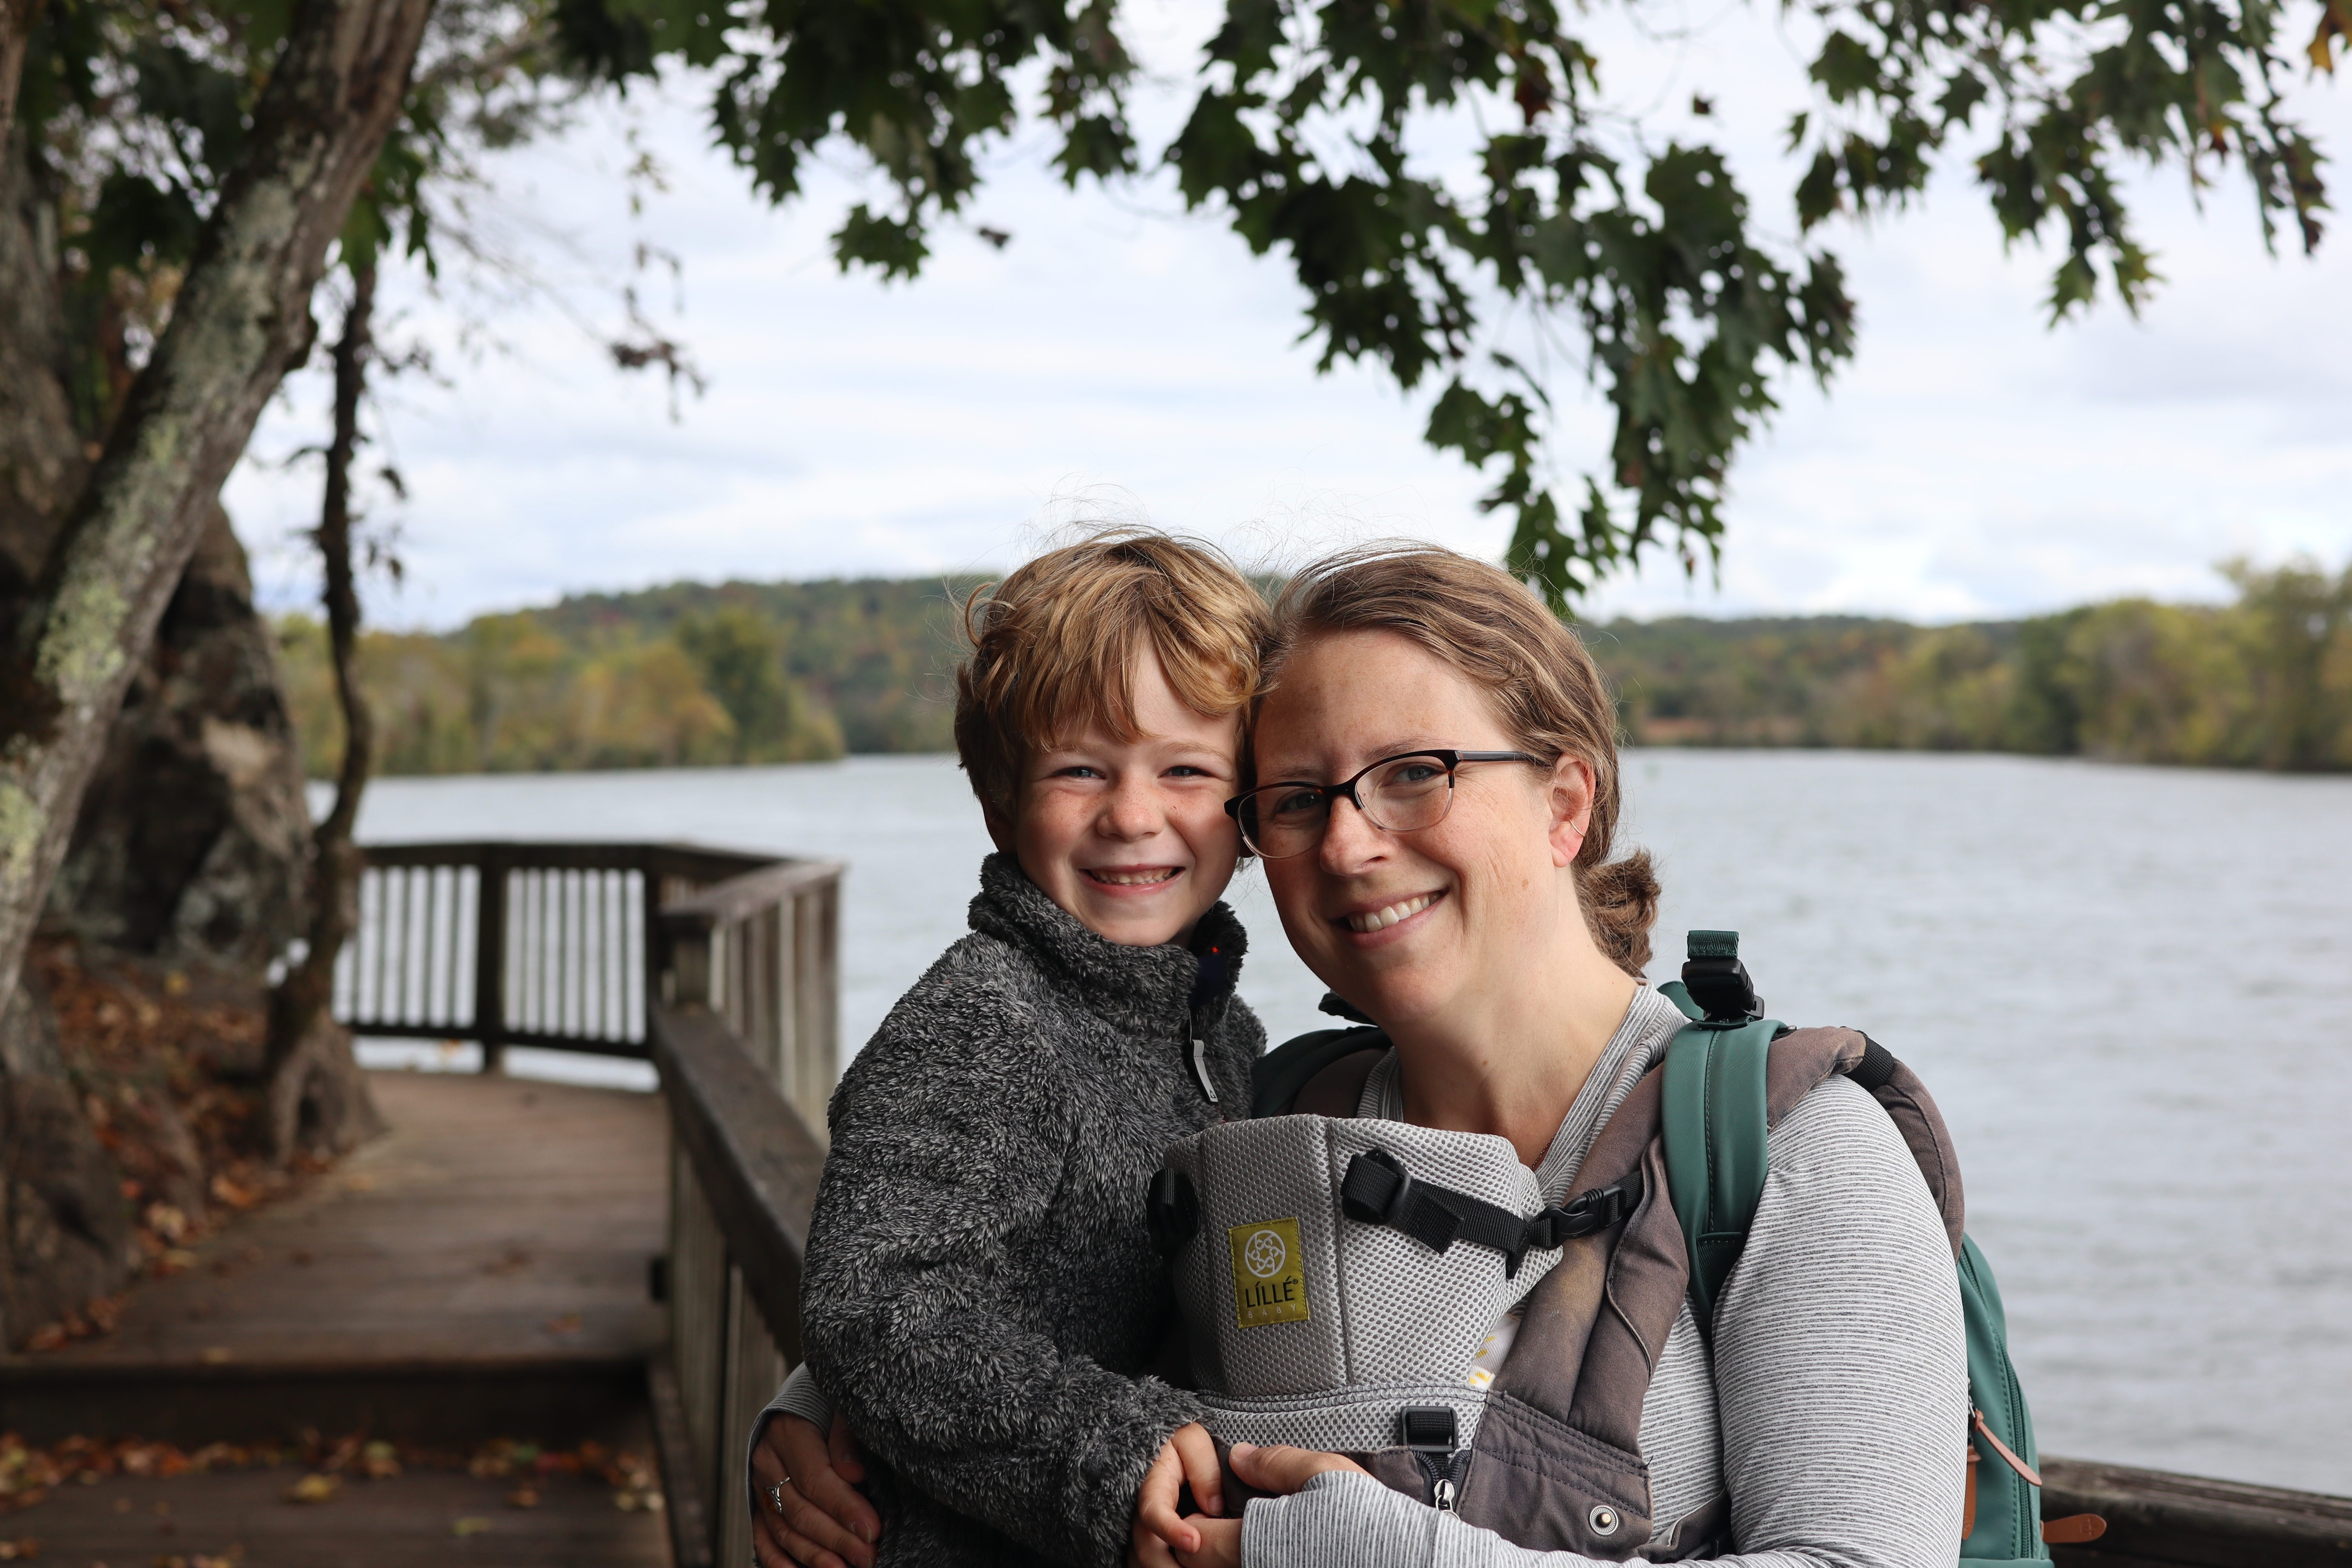
\includegraphics[keepaspectratio]{img/katie-jo-riverside.jpeg}}

}

\caption{Photo credit to Katie and Joshua Rosenberg}

\end{figure}%

\subsection{Key Characteristics}\label{key-characteristics-2}

\begin{longtable}[]{@{}
  >{\raggedright\arraybackslash}p{(\linewidth - 2\tabcolsep) * \real{0.5294}}
  >{\raggedright\arraybackslash}p{(\linewidth - 2\tabcolsep) * \real{0.4706}}@{}}
\toprule\noalign{}
\begin{minipage}[b]{\linewidth}\raggedright
\textbf{Characteristic}
\end{minipage} & \begin{minipage}[b]{\linewidth}\raggedright
\textbf{Details}
\end{minipage} \\
\midrule\noalign{}
\endhead
\bottomrule\noalign{}
\endlastfoot
Time Estimate & 45 minutes - 1.5 hours \\
Trail Distance (Miles) & 1.03 \\
Elevation Change & Moderate \\
Pets & Allowed on leash \\
Parking Pass/Entrance Fee & Required (pay on site) \\
Restroom(s) & Yes \\
Best Ages & Toddlers and Little Kids \\
Strollers and Wheelchairs & Not accessible \\
\end{longtable}

\pandocbounded{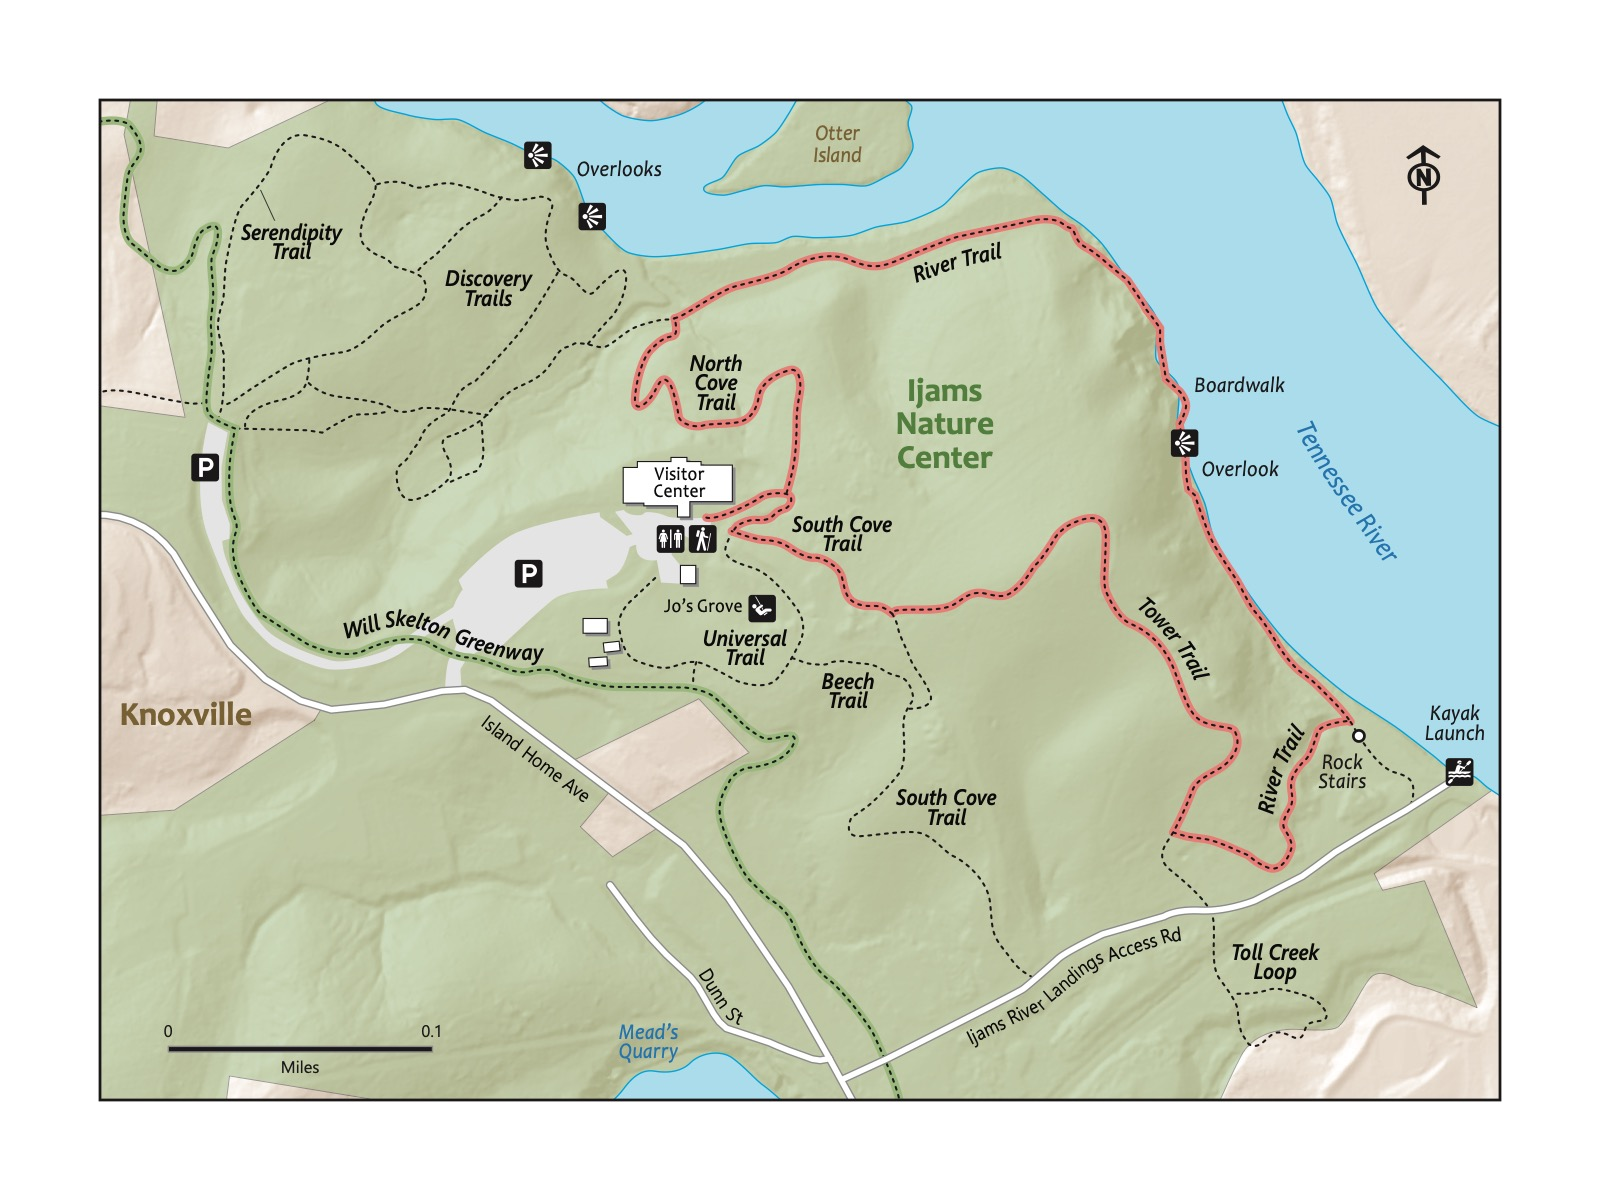
\includegraphics[keepaspectratio]{maps/trail-02-map.jpeg}}

\subsection{Directions to the
Trailhead}\label{directions-to-the-trailhead-1}

Trailhead Address: Ijams Nature Center, 2915 Island Home Ave, Knoxville,
TN 37920

Trailhead GPS Coordinates: 35.95612, -83.86725

Use the above address to easily navigate to the parking area. Park in
the large parking lot near the Visitor's Center.

\begin{tcolorbox}[enhanced jigsaw, colback=white, colframe=quarto-callout-note-color-frame, breakable, opacityback=0, toprule=.15mm, bottomrule=.15mm, rightrule=.15mm, left=2mm, leftrule=.75mm, arc=.35mm]
\begin{minipage}[t]{5.5mm}
\textcolor{quarto-callout-note-color}{\faInfo}
\end{minipage}%
\begin{minipage}[t]{\textwidth - 5.5mm}

\vspace{-3mm}\textbf{Blue Phlox}\vspace{3mm}

Blue Phlox is a native wildflower that blooms in early to mid-spring.
These plants provide an important source of early-season nectar for
pollinators, like the swallowtail butterfly and other native moths.
-MaryRose Weatherton

\end{minipage}%
\end{tcolorbox}

\subsection{Trail Description}\label{trail-description-1}

\begin{longtable}[]{@{}
  >{\raggedright\arraybackslash}p{(\linewidth - 2\tabcolsep) * \real{0.2639}}
  >{\raggedright\arraybackslash}p{(\linewidth - 2\tabcolsep) * \real{0.7361}}@{}}
\toprule\noalign{}
\begin{minipage}[b]{\linewidth}\raggedright
Distance from Start
\end{minipage} & \begin{minipage}[b]{\linewidth}\raggedright
Description
\end{minipage} \\
\midrule\noalign{}
\endhead
\bottomrule\noalign{}
\endlastfoot
0.0 & Start near the doors to the Visitor's Center and access the trail
via the wooden steps. \\
0.05 & Turn left to begin the North Cove Trail. \\
0.2 & Turn right onto the River Trail. \\
0.4 & Short wooden stairs down to the boardwalk section. \\
0.5 & End of the boardwalk section. \\
0.6 & Climb rock steps. \\
0.7 & Turn right on the Tower Trail (or, optionally, remain on the River
Trail to head toward Mead's Quarry). \\
0.85 & Pass an old communication tower at the high point of the trail;
begin to descend back to the Visitor's Center. \\
1.03 & Return to the Visitor's Center. \\
\end{longtable}

\subsection{Nearby}\label{nearby-1}

\begin{itemize}
\tightlist
\item
  \textbf{Visiting Jo's Grove near the Visitor's Center.} This area
  which features a fun cabin and a wooded area for kids to play (this is
  a premiere hide-and-seek spot!**
\item
  \textbf{Grabbing a bite to eat on the south side of Knoxville!} Our
  favorites include South Coast Pizza (1103 Sevier Ave, Knoxville, TN
  37920) and Angry Dumplings Tea (1119 Sevier Ave, Knoxville, TN 37920).
  Breweries nearby also abound, as well as Suttree Landing Park, which
  boasts a very fun playground.
\item
  \textbf{Seeing more of what Ijams has to offer}. Check by checking out
  the Ijams Crag hike across the road at Mead' Quary!
\end{itemize}

\chapter{Trail 3: Lakeshore Park}\label{trail-3-lakeshore-park}

\subsection{Overview}\label{overview-3}

A gem in Knoxville's city park system, this hike, entirely on a paved
path, circles the perimeter of the park, featuring high points, views of
the Smokies, and a boardwalk along the river. It also boasts four
excellent play areas along the way! Well known, but not overrated, this
is a great spot for a hike that could fit into a busy weekend, or even a
weeknight, and is great for young ones of all ages, truly offering
something for everyone.

\begin{figure}[H]

{\centering \pandocbounded{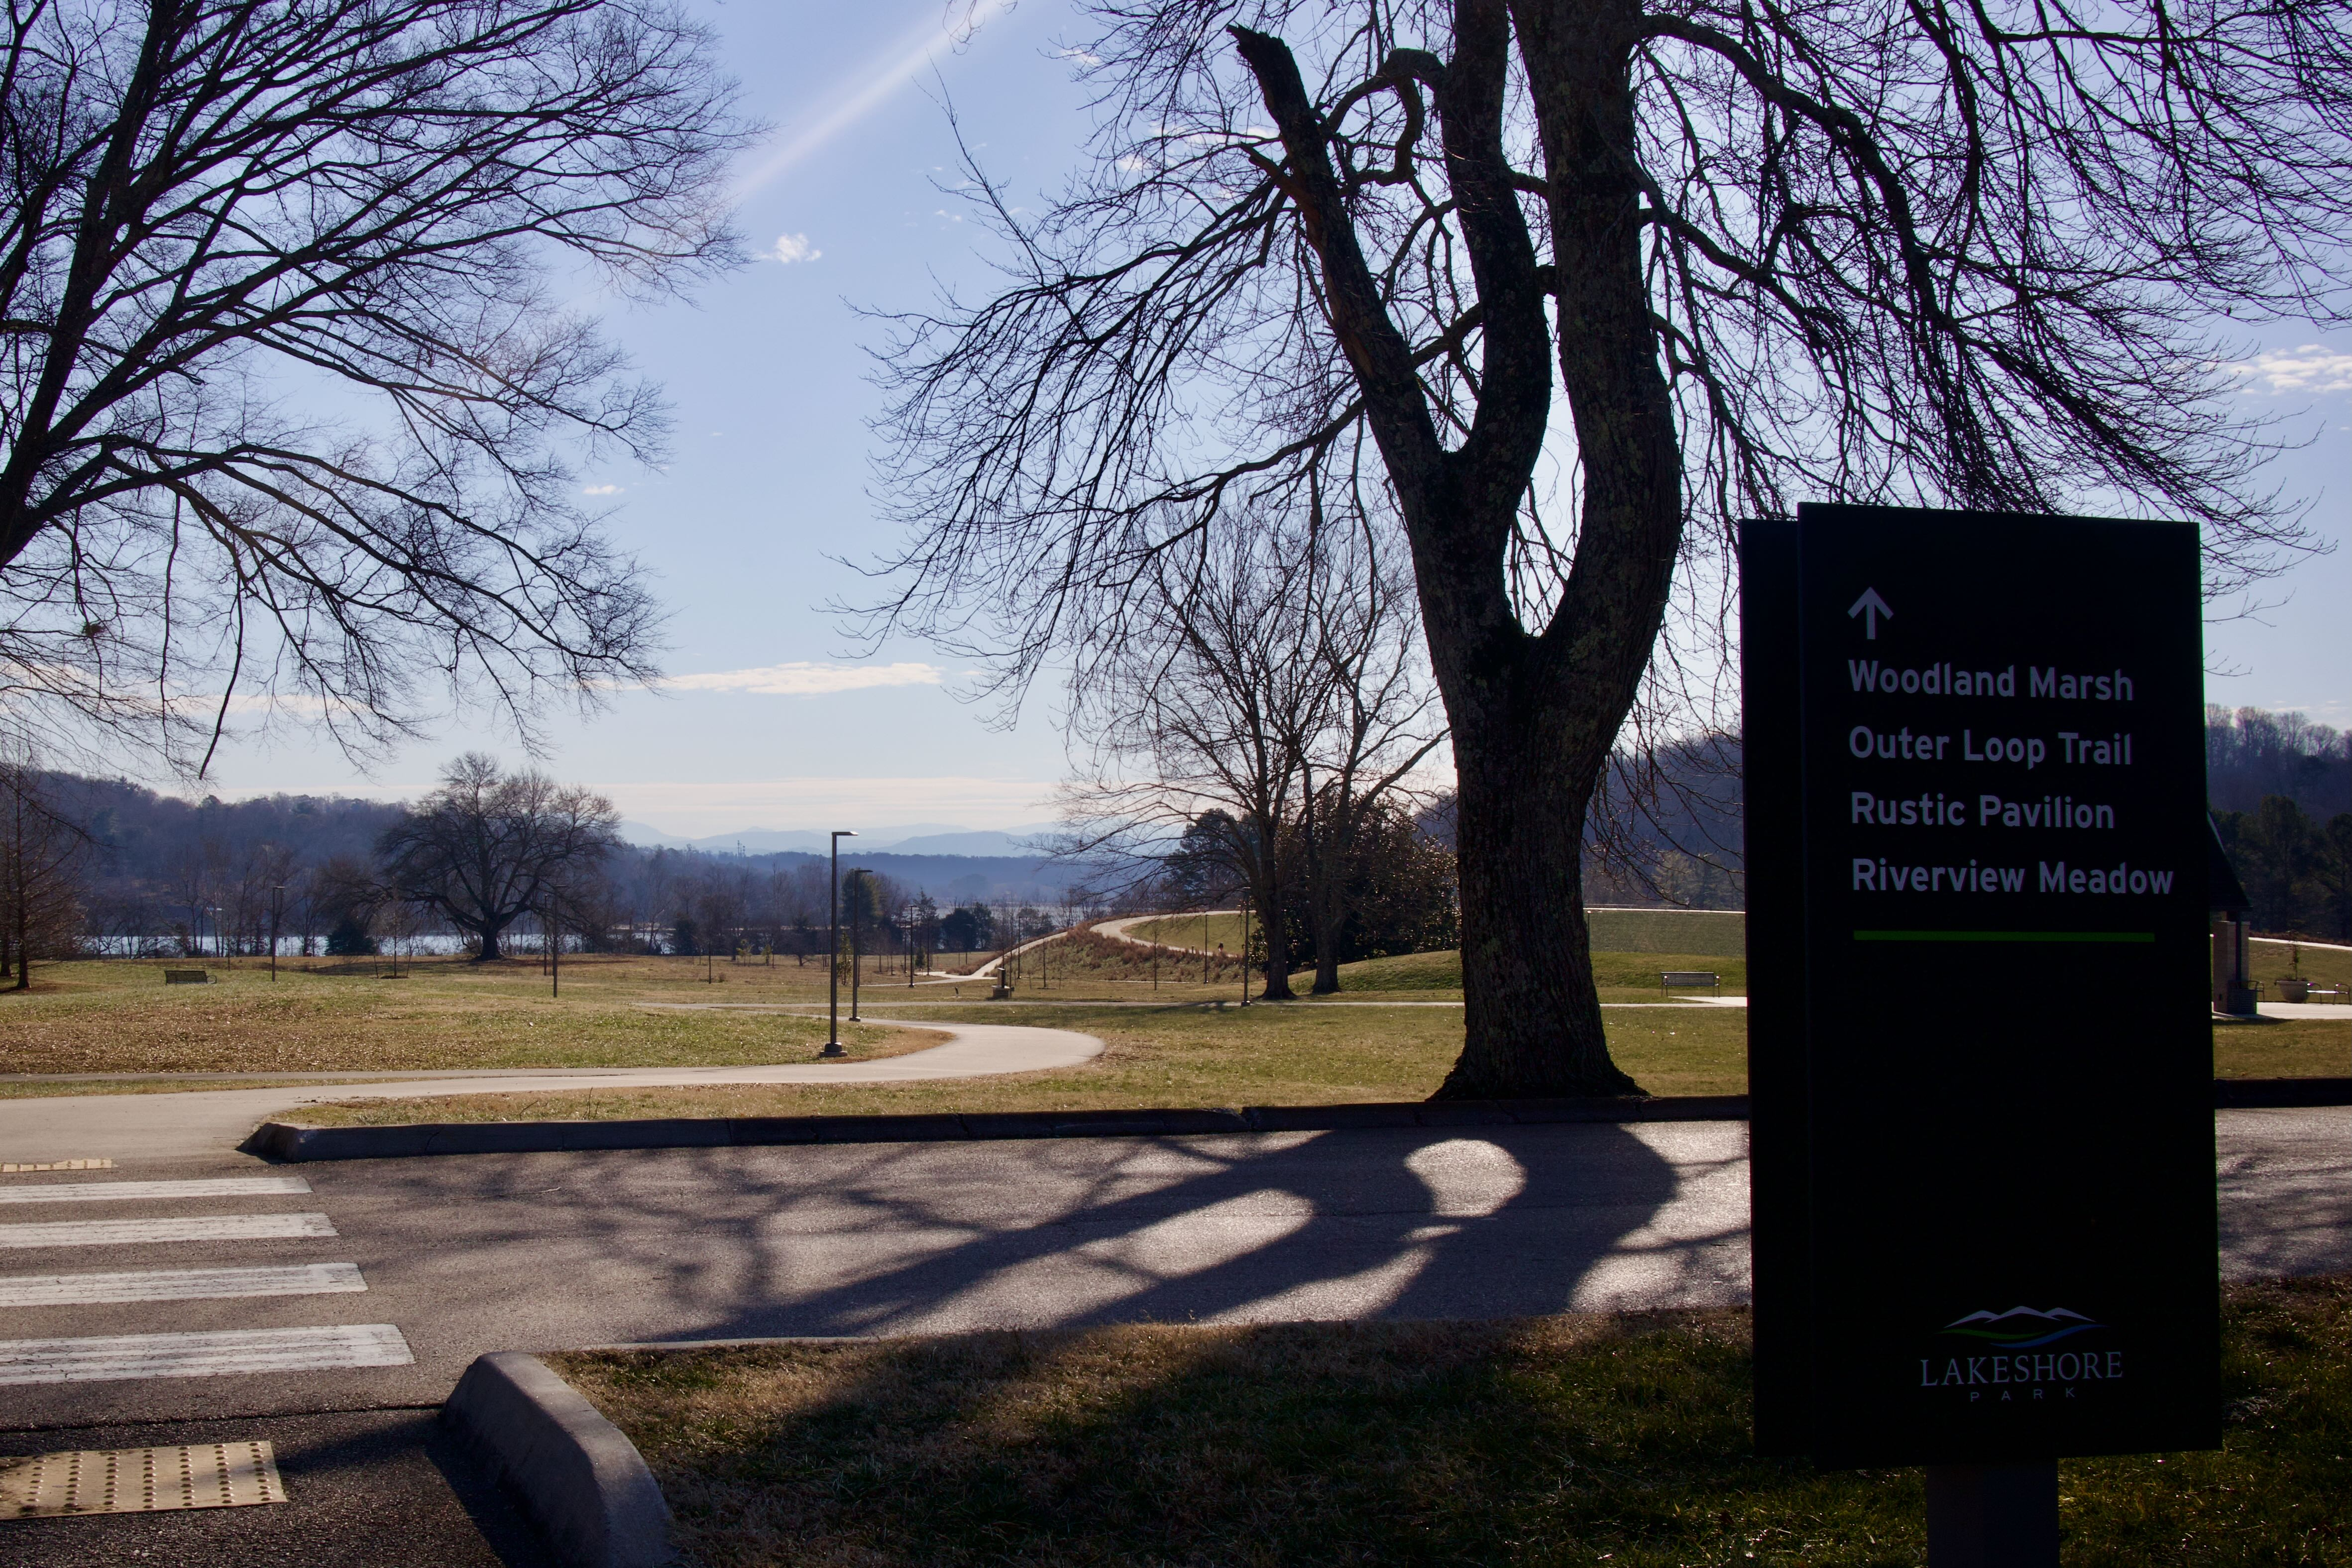
\includegraphics[keepaspectratio]{img/lakeshore-new.jpeg}}

}

\caption{Photo credit to Katie and Joshua Rosenberg}

\end{figure}%

\subsection{Key Characteristics}\label{key-characteristics-3}

\begin{longtable}[]{@{}
  >{\raggedright\arraybackslash}p{(\linewidth - 2\tabcolsep) * \real{0.5400}}
  >{\raggedright\arraybackslash}p{(\linewidth - 2\tabcolsep) * \real{0.4600}}@{}}
\toprule\noalign{}
\begin{minipage}[b]{\linewidth}\raggedright
\textbf{Characteristic}
\end{minipage} & \begin{minipage}[b]{\linewidth}\raggedright
\textbf{Details}
\end{minipage} \\
\midrule\noalign{}
\endhead
\bottomrule\noalign{}
\endlastfoot
Time Estimate & 1.5 hours - 2.5 hours \\
Trail Distance (Miles) & 2.2 \\
Elevation Change & Gentle \\
Pets & Allowed on leash \\
Parking Pass/Entrance Fee & Not Required \\
Restroom(s) & Yes \\
Best Ages & Toddlers, Little Kids, and Big Kids \\
Strollers and Wheelchairs & Not accessible \\
\end{longtable}

\pandocbounded{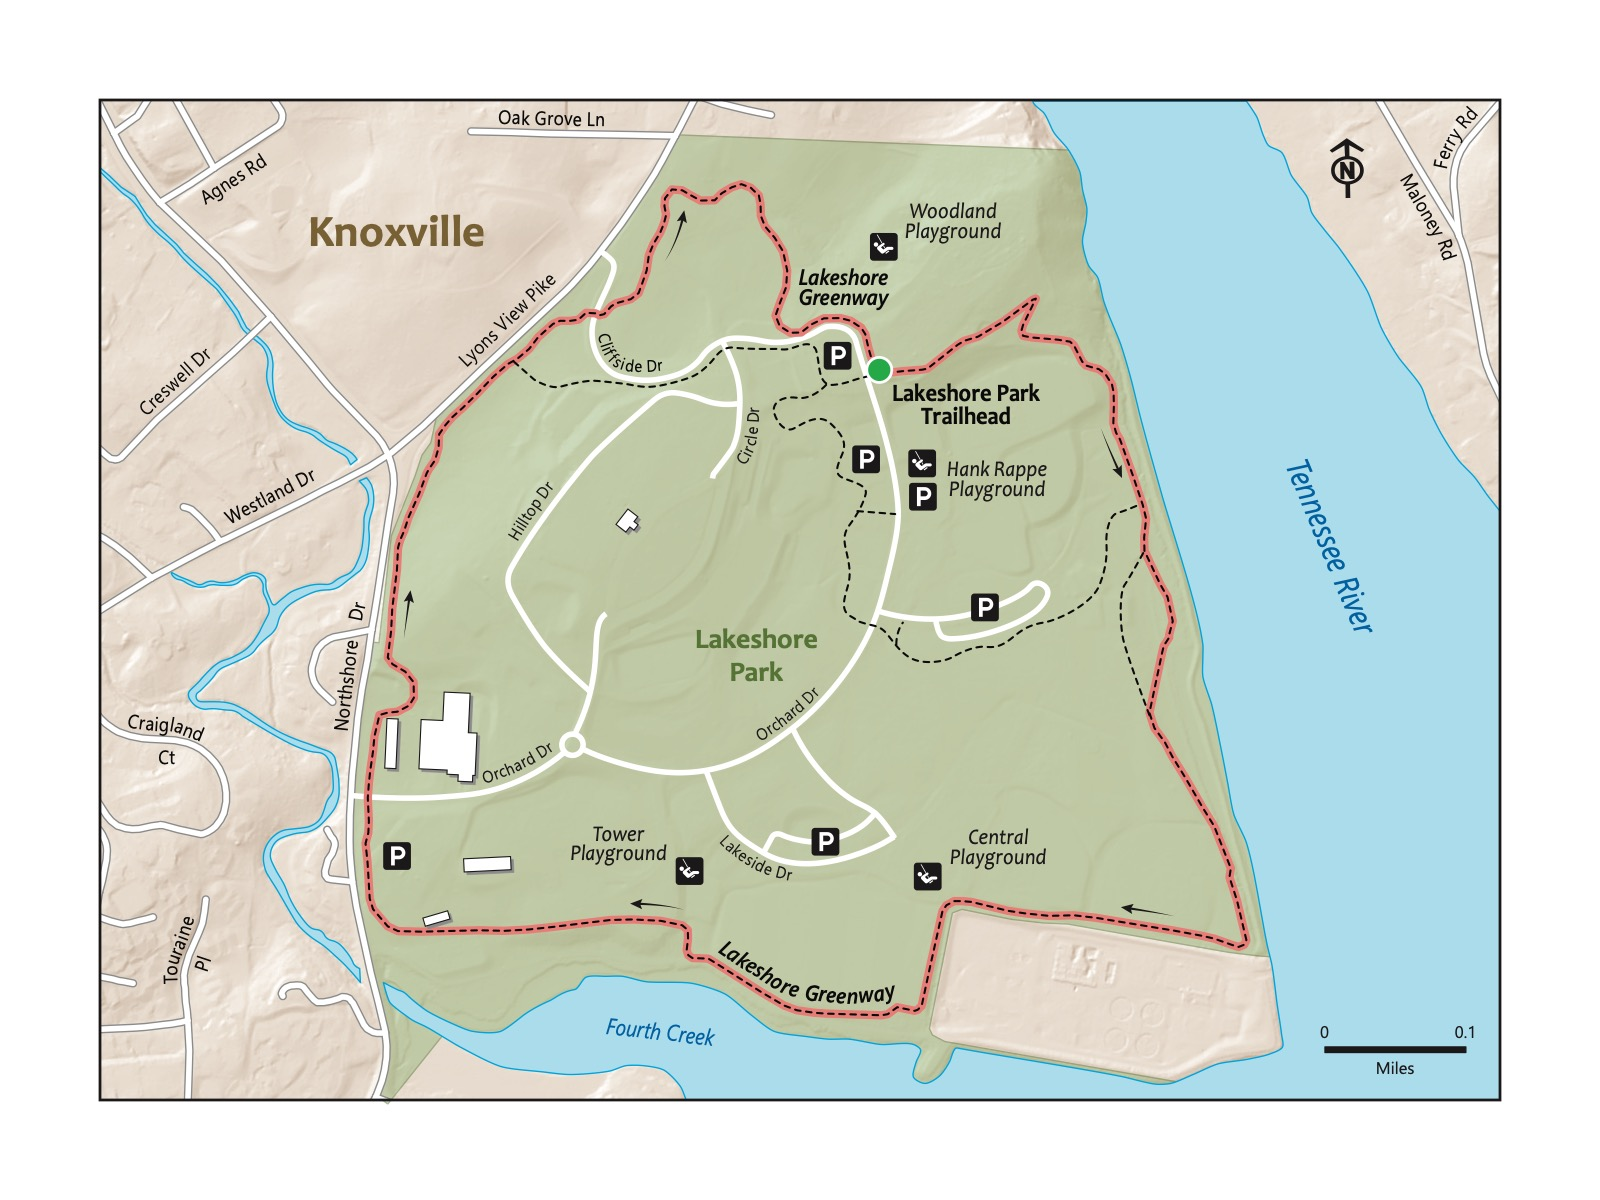
\includegraphics[keepaspectratio]{maps/trail-03-map.jpeg}}

\subsection{Directions to the
Trailhead}\label{directions-to-the-trailhead-2}

Trailhead Address: Lakeshore Park, 6014 Lyons View Pike, Knoxville, TN
37919

Trailhead GPS Coordinates: 35.92389, -83.990

The address above navigates to the park's main entrance. Our hike starts
at a large parking area near the center of the park. To find it,
entering Lakeshore from Lyons View Pike, turn onto Cliffside Dr.~and
park in the large parking area on the right, immediately past Circle
Dr.~Start on the greenway near the parking lot on the same side of the
road on which you are parked. Of course, you can park elsewhere nearby
or in any parking area at Lakeshore.

\subsection{Trail Description}\label{trail-description-2}

\begin{longtable}[]{@{}
  >{\raggedright\arraybackslash}p{(\linewidth - 2\tabcolsep) * \real{0.1193}}
  >{\raggedright\arraybackslash}p{(\linewidth - 2\tabcolsep) * \real{0.8807}}@{}}
\toprule\noalign{}
\begin{minipage}[b]{\linewidth}\raggedright
Distance from Start
\end{minipage} & \begin{minipage}[b]{\linewidth}\raggedright
Description
\end{minipage} \\
\midrule\noalign{}
\endhead
\bottomrule\noalign{}
\endlastfoot
0.0 & Cross Orchard Drive, heading clockwise on the paved greenway. Note
the greenway on the left, which immediately heads toward the Huie
Woodland Playground. \\
0.05 & Bench and overlook to the Smokies. Can you spy Clingman's Dome?
Note that Hank Rappé playground is immediately below the greenway (to
your right). \\
0.15 & Short, steep descent! \\
0.4 & Optional boardwalk section (recommended!). Check out the viewing
platform overlooking the Tennessee River around 200 feet ahead on the
left. \\
0.5 & Boardwalk and the primary greenway reconnect. \\
0.9 & Central Playground on the right. \\
1.2 & Tower Playground on the right. \\
1.5 & Ascent (followed by a little hill back down) begins. \\
2.2 & Traihead. \\
\end{longtable}

\begin{tcolorbox}[enhanced jigsaw, colback=white, colframe=quarto-callout-note-color-frame, breakable, opacityback=0, toprule=.15mm, bottomrule=.15mm, rightrule=.15mm, left=2mm, leftrule=.75mm, arc=.35mm]
\begin{minipage}[t]{5.5mm}
\textcolor{quarto-callout-note-color}{\faInfo}
\end{minipage}%
\begin{minipage}[t]{\textwidth - 5.5mm}

\vspace{-3mm}\textbf{Appalachian Trail}\vspace{3mm}

Surprisingly, the crest of the Smokies (and the Appalachian Trail) are
visible from this park. The Appalachian Trail is more than 2,100 miles
long, beginning at Springer Mountain, Georgia, and ending at Mount
Katahdin, in Maine. The longest section without a road crossing is in
the Smokies -- from Fontana Dam to Newfound Gap.\\

\end{minipage}%
\end{tcolorbox}

\subsection{Nearby}\label{nearby-2}

\begin{figure}[H]

{\centering \pandocbounded{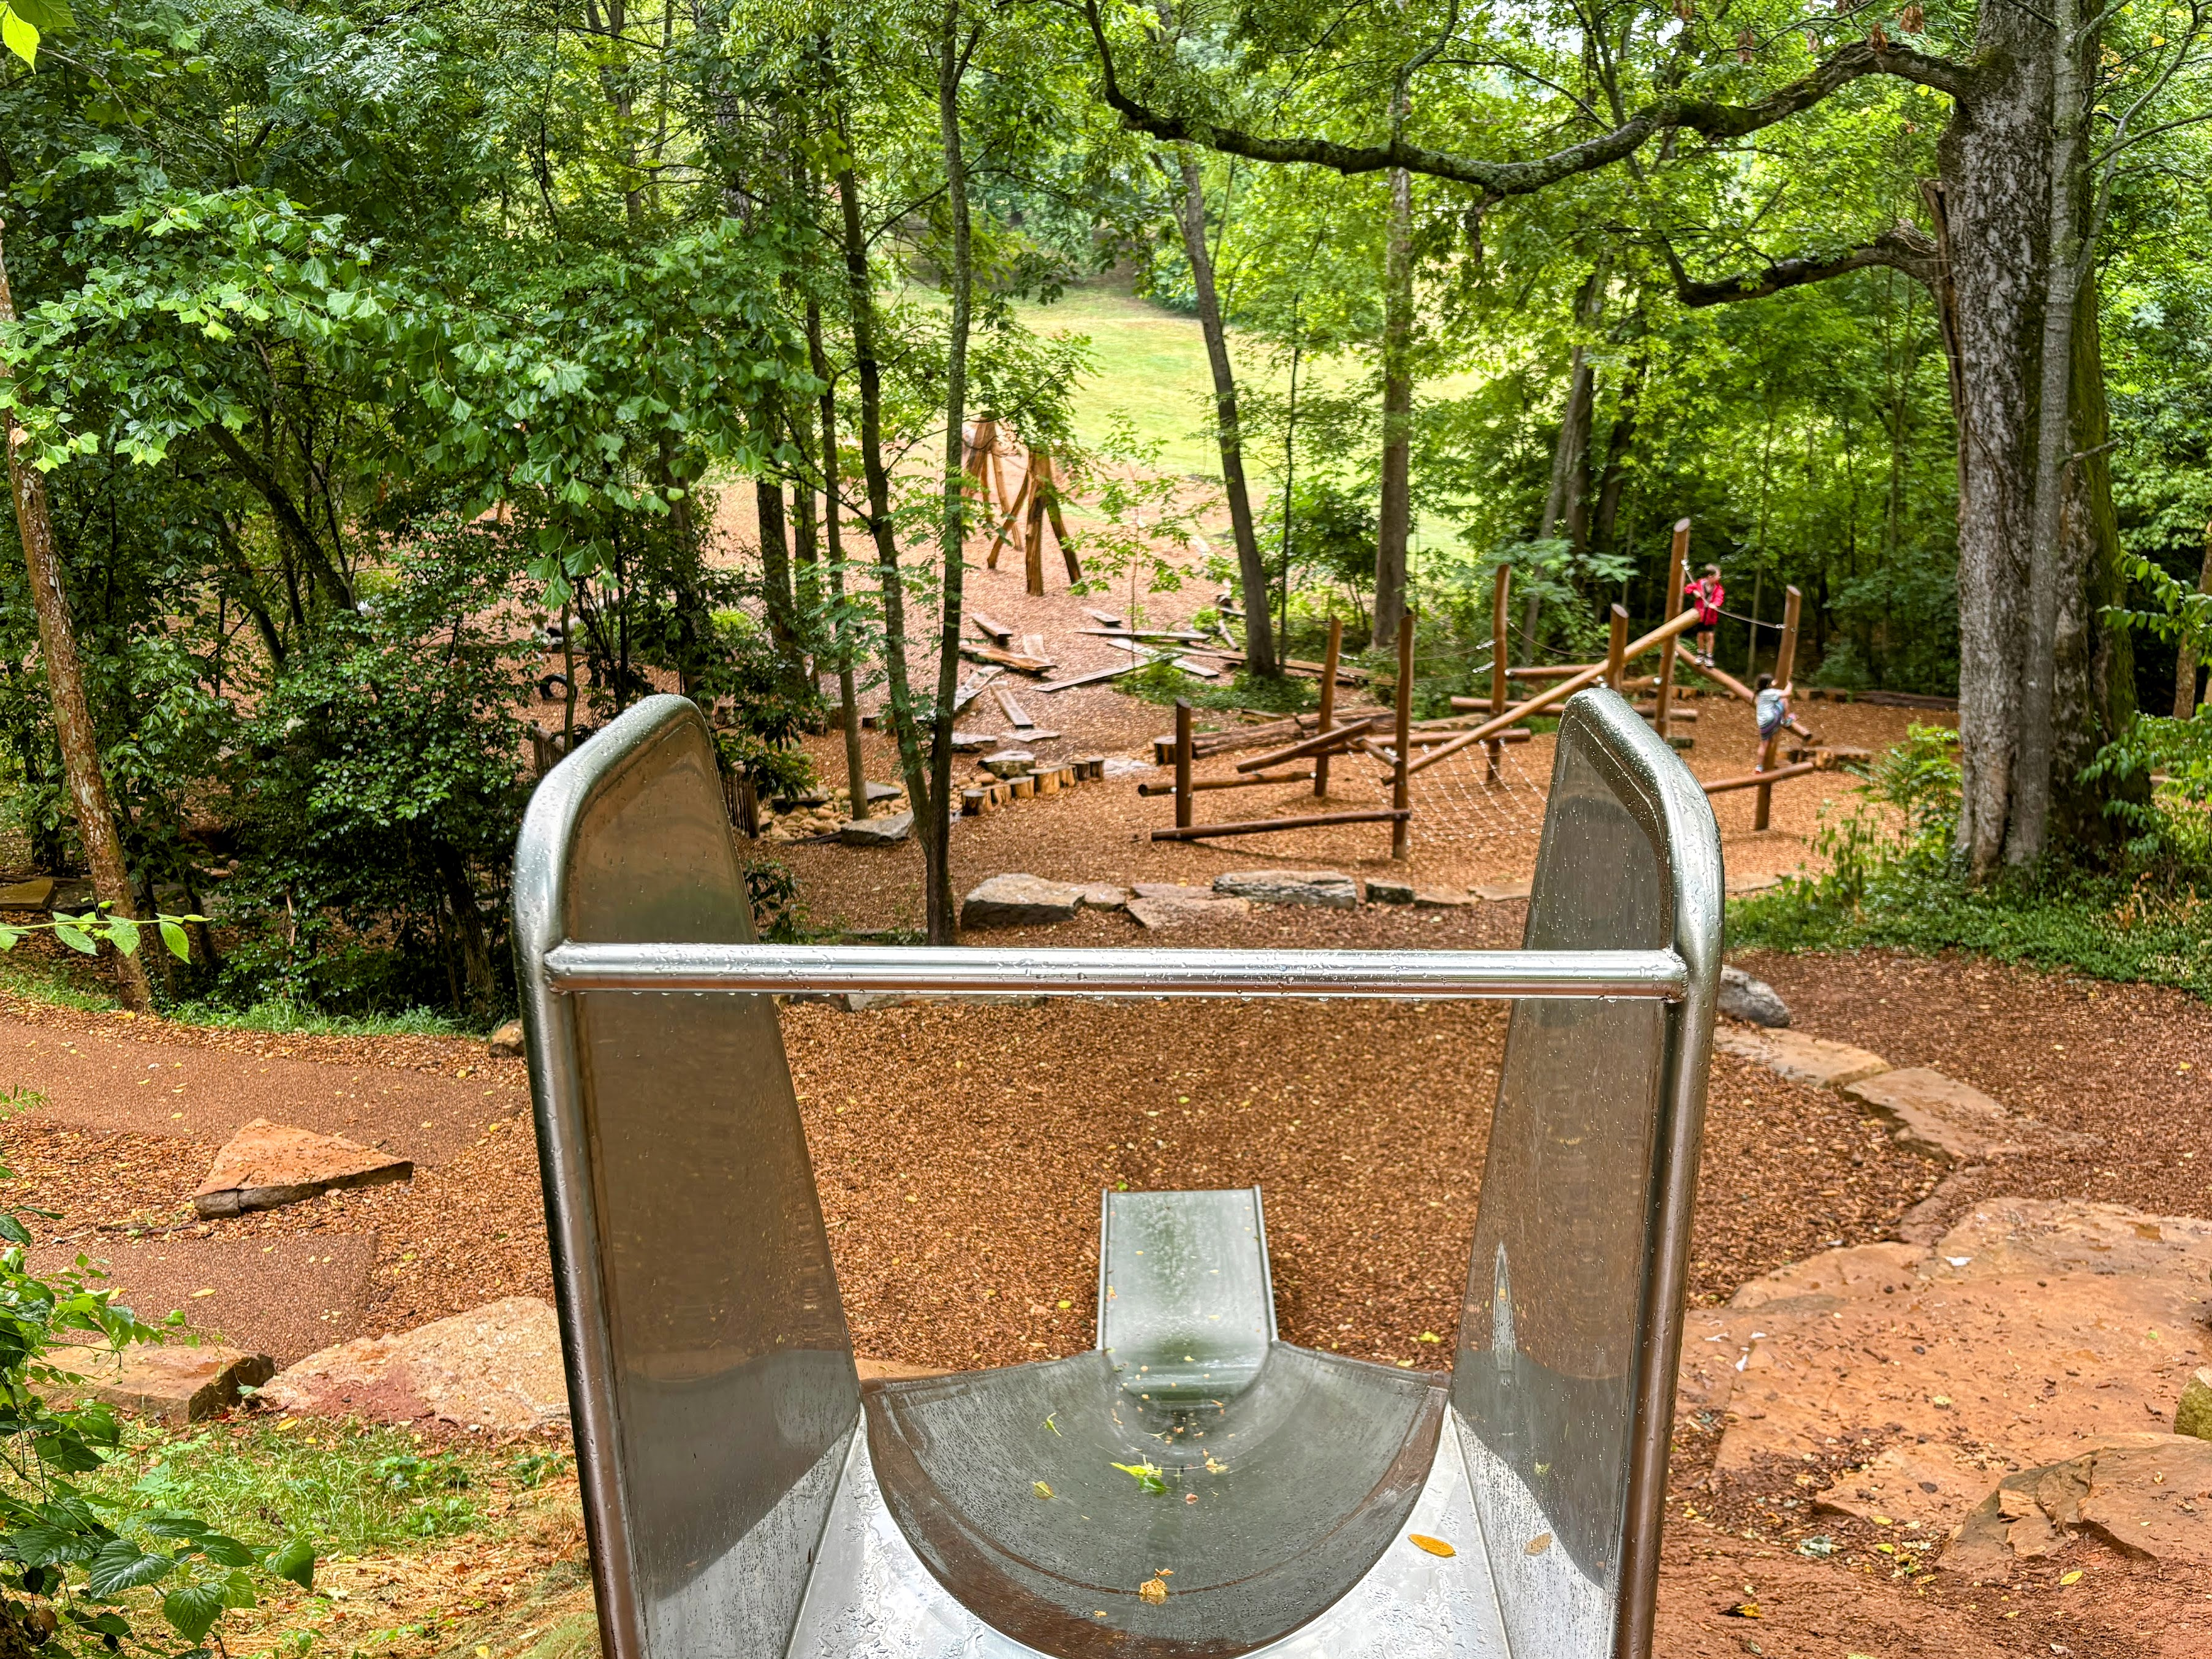
\includegraphics[keepaspectratio]{img/huie.jpg}}

}

\caption{Photo credit to Katie and Joshua Rosenberg}

\end{figure}%

\begin{itemize}
\tightlist
\item
  \textbf{Enjoy one or more of the many playgrounds!} There are four
  awesome playgrounds at Lakeshore: Hank Rappé (universal playground
  with a bit of everything), Huie Woodland (nature-themed), Tower (lots
  of climbing opportunities, best for kids age 5 and older), and Central
  (best suited for ages 5 and older, and with workout equipment nearby
  for adults).
\item
  \textbf{Bring a picnic!} Lakeshore seems made for picnics. Enjoy one
  on a grassy area or one numerous seating areas near the Hank Rappé,
  Tower, and Central playgrounds.
\end{itemize}

\chapter{Trail 4: High Ground Park}\label{trail-4-high-ground-park}

\subsection{Overview}\label{overview-4}

This is one of the closest hikes to the city center of Knoxville, and
it's stroller-friendly! This short but sweet hike is perfect as a real
but accessible outing for toddlers and little kids. The red chairs at
the top are a fun stopping point. The deep woods are pretty and offer
something new in each season. This could be a great first hike for
toddlers -- it was one of the first for our little one, and made us feel
like we could start venturing to other regional hiking destinations.

\begin{figure}[H]

{\centering \pandocbounded{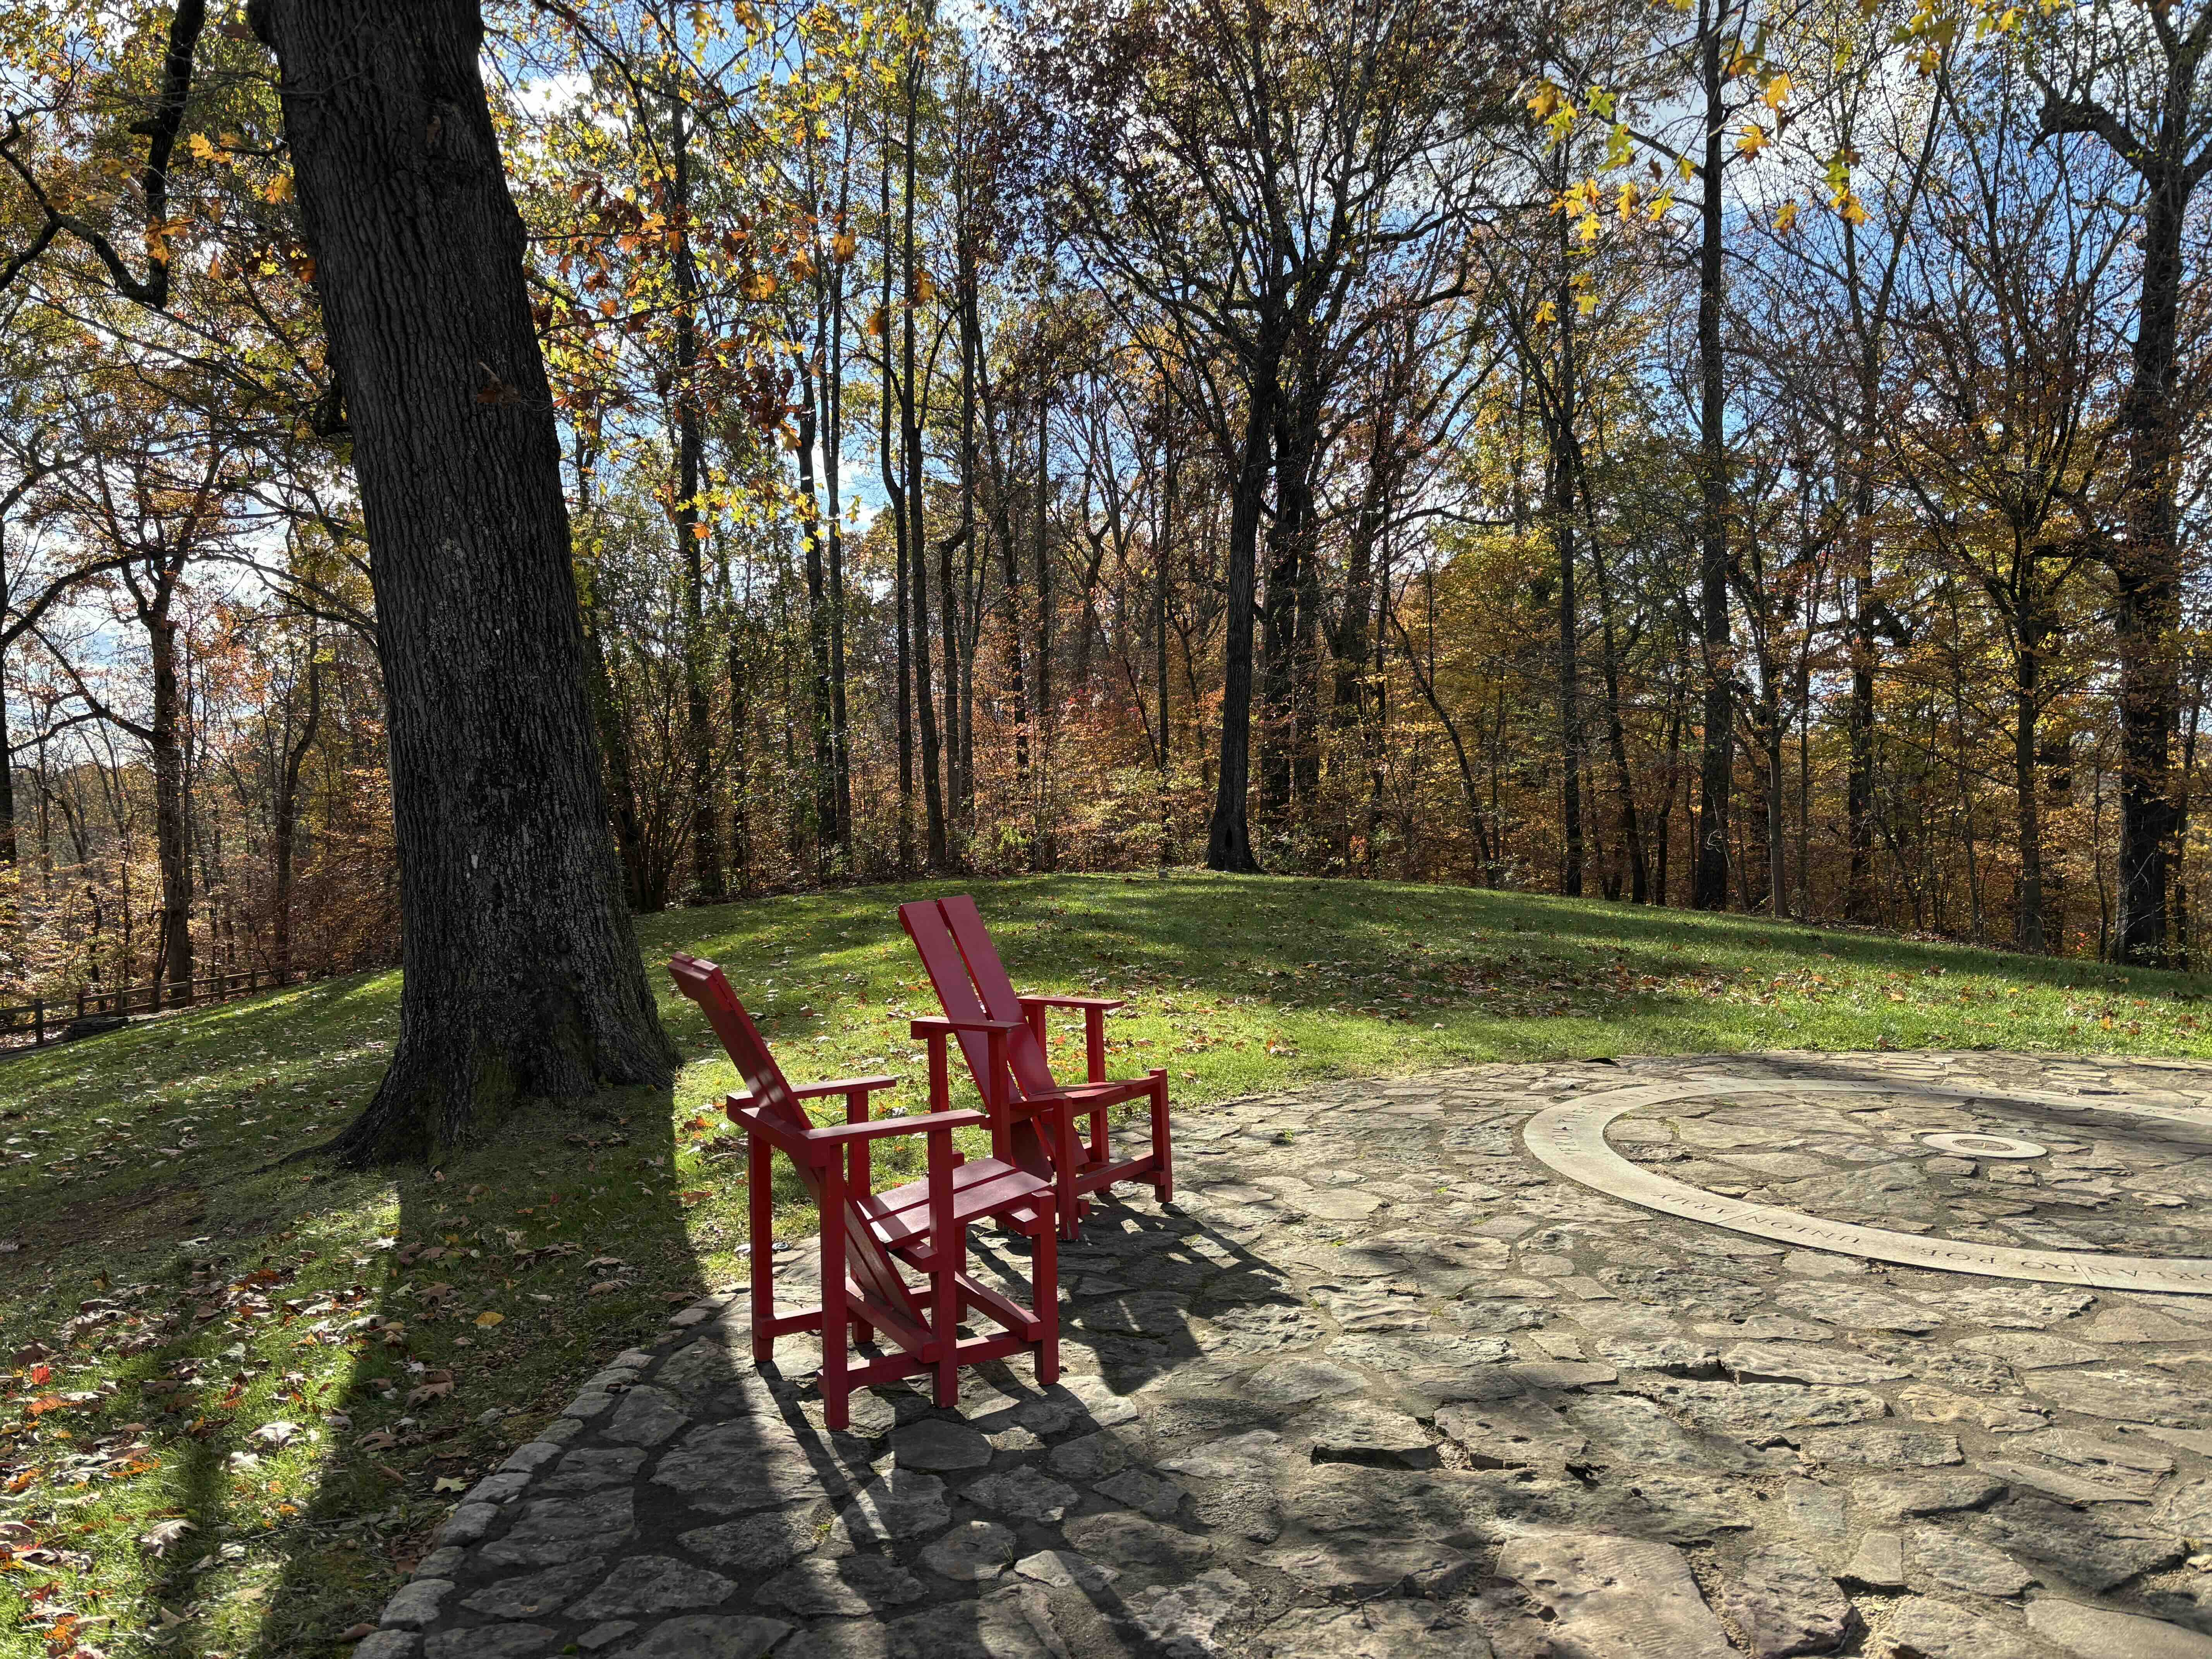
\includegraphics[keepaspectratio]{img/trail-04-figure-01.jpg}}

}

\caption{Photo credit to Katie and Joshua Rosenberg}

\end{figure}%

\subsection{Key Characteristics}\label{key-characteristics-4}

\begin{longtable}[]{@{}
  >{\raggedright\arraybackslash}p{(\linewidth - 2\tabcolsep) * \real{0.5745}}
  >{\raggedright\arraybackslash}p{(\linewidth - 2\tabcolsep) * \real{0.4255}}@{}}
\toprule\noalign{}
\begin{minipage}[b]{\linewidth}\raggedright
\textbf{Characteristic}
\end{minipage} & \begin{minipage}[b]{\linewidth}\raggedright
\textbf{Details}
\end{minipage} \\
\midrule\noalign{}
\endhead
\bottomrule\noalign{}
\endlastfoot
Time Estimate & 0.5 hours - 1 hour \\
Trail Distance (Miles) & 0.7 \\
Elevation Change & Gentle \\
Pets & Allowed on leash \\
Parking Pass/Entrance Fee & Not Required \\
Restroom(s) & No \\
Best Ages & Toddlers and Little kids \\
Strollers and Wheelchairs & Accessible \\
\end{longtable}

\pandocbounded{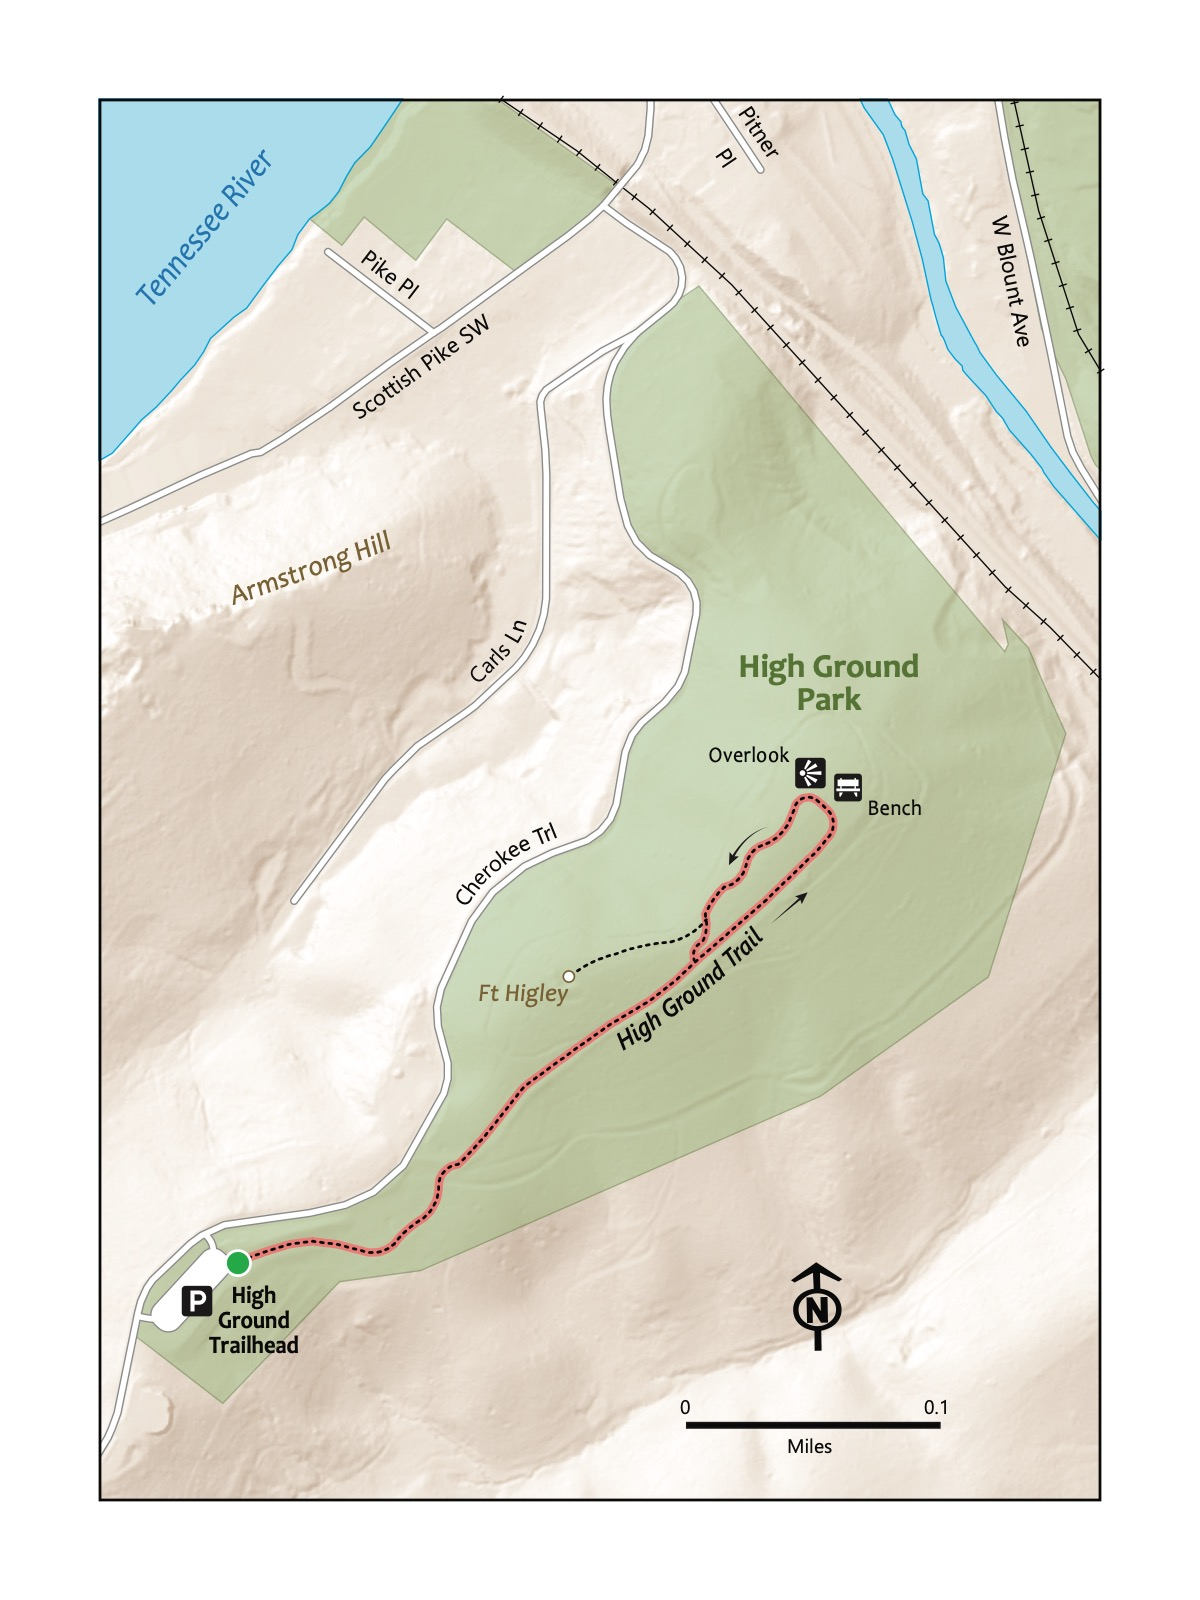
\includegraphics[keepaspectratio]{maps/trail-04-map.jpeg}}

\subsection{Directions to the
Trailhead}\label{directions-to-the-trailhead-3}

Trailhead Address: High Ground Park, 1000 Cherokee Trail, Knoxville, TN
37920

Trailhead GPS Coordinates: 35.93824, -83.9258

The trail begins from the parking lot at the above address; look for the
paved path near the back of the parking lot. You can't miss it!

\begin{tcolorbox}[enhanced jigsaw, colback=white, colframe=quarto-callout-note-color-frame, breakable, opacityback=0, toprule=.15mm, bottomrule=.15mm, rightrule=.15mm, left=2mm, leftrule=.75mm, arc=.35mm]
\begin{minipage}[t]{5.5mm}
\textcolor{quarto-callout-note-color}{\faInfo}
\end{minipage}%
\begin{minipage}[t]{\textwidth - 5.5mm}

\vspace{-3mm}\textbf{Earthworks}\vspace{3mm}

Structures formed from shaping rocks and soil, often as part of forts
around Knoxville constructed during the Civil War. Surprisingly
long-standing. The earthworks here and at the nearby Fort Dickerson
include ramparts -- small hills or banks that served as defensive walls.

\end{minipage}%
\end{tcolorbox}

\subsection{Trail Description}\label{trail-description-3}

\begin{longtable}[]{@{}
  >{\raggedright\arraybackslash}p{(\linewidth - 2\tabcolsep) * \real{0.2361}}
  >{\raggedright\arraybackslash}p{(\linewidth - 2\tabcolsep) * \real{0.7639}}@{}}
\toprule\noalign{}
\begin{minipage}[b]{\linewidth}\raggedright
Distance from Start
\end{minipage} & \begin{minipage}[b]{\linewidth}\raggedright
Description
\end{minipage} \\
\midrule\noalign{}
\endhead
\bottomrule\noalign{}
\endlastfoot
0 & Start off on the trail with a gentle descent. \\
0.1 & Enter the wooded part of the hike and begin a gentle climb. \\
0.35 & Red chairs and the large open area. Head toward the mowed grassy
section. \\
0.4 & Look for a spur trail that heads to the site of the Fort Higley
earthworks, constructed during the Civil War by Union forces. \\
0.7 & Traihead. \\
\end{longtable}

\subsection{Nearby}\label{nearby-3}

\begin{itemize}
\tightlist
\item
  \textbf{Stop by a fun food hall before or after!} The nearby Kern's
  Food Hall (2201 Kerns Rising Way, Knoxville, TN 37920) has a good
  range of options and an outdoor play area for kids to romp around.
\item
  \textbf{For more outdoor fun, hike the nearby River Bluff Wildlife
  area.} The nearby River Bluff Wildlife Area is an interesting
  counterbalance to the ease of High Ground Park. it features a short
  but rustic hike to a pretty overlook of the city.**** Visit
  Knoxville's website (\url{https://www.visitknoxville.com/}) has more
  information and a nice map.
\end{itemize}

\chapter{Trail 5: UT Arboretum}\label{trail-5-ut-arboretum}

\subsection{Overview}\label{overview-5}

This is a gem of a hike that is off the radar for many in Knoxville, as
it is tucked away in nearby Oak Ridge. Start your hike at a trailhead
that offers many hiking options. We recommend walking up the paved path
past botanical specimens, including ``unique conifers''! Circle around
park facilities past a pretty field and forests. Upon returning to the
start, there are other trails to the different ecological zones
represented in an area that is worth a visit; we like the trails near
the marshy area with the clear creek, perfect for splashing in warm
weather. Suitable for kids of all ages.

\begin{figure}[H]

{\centering \pandocbounded{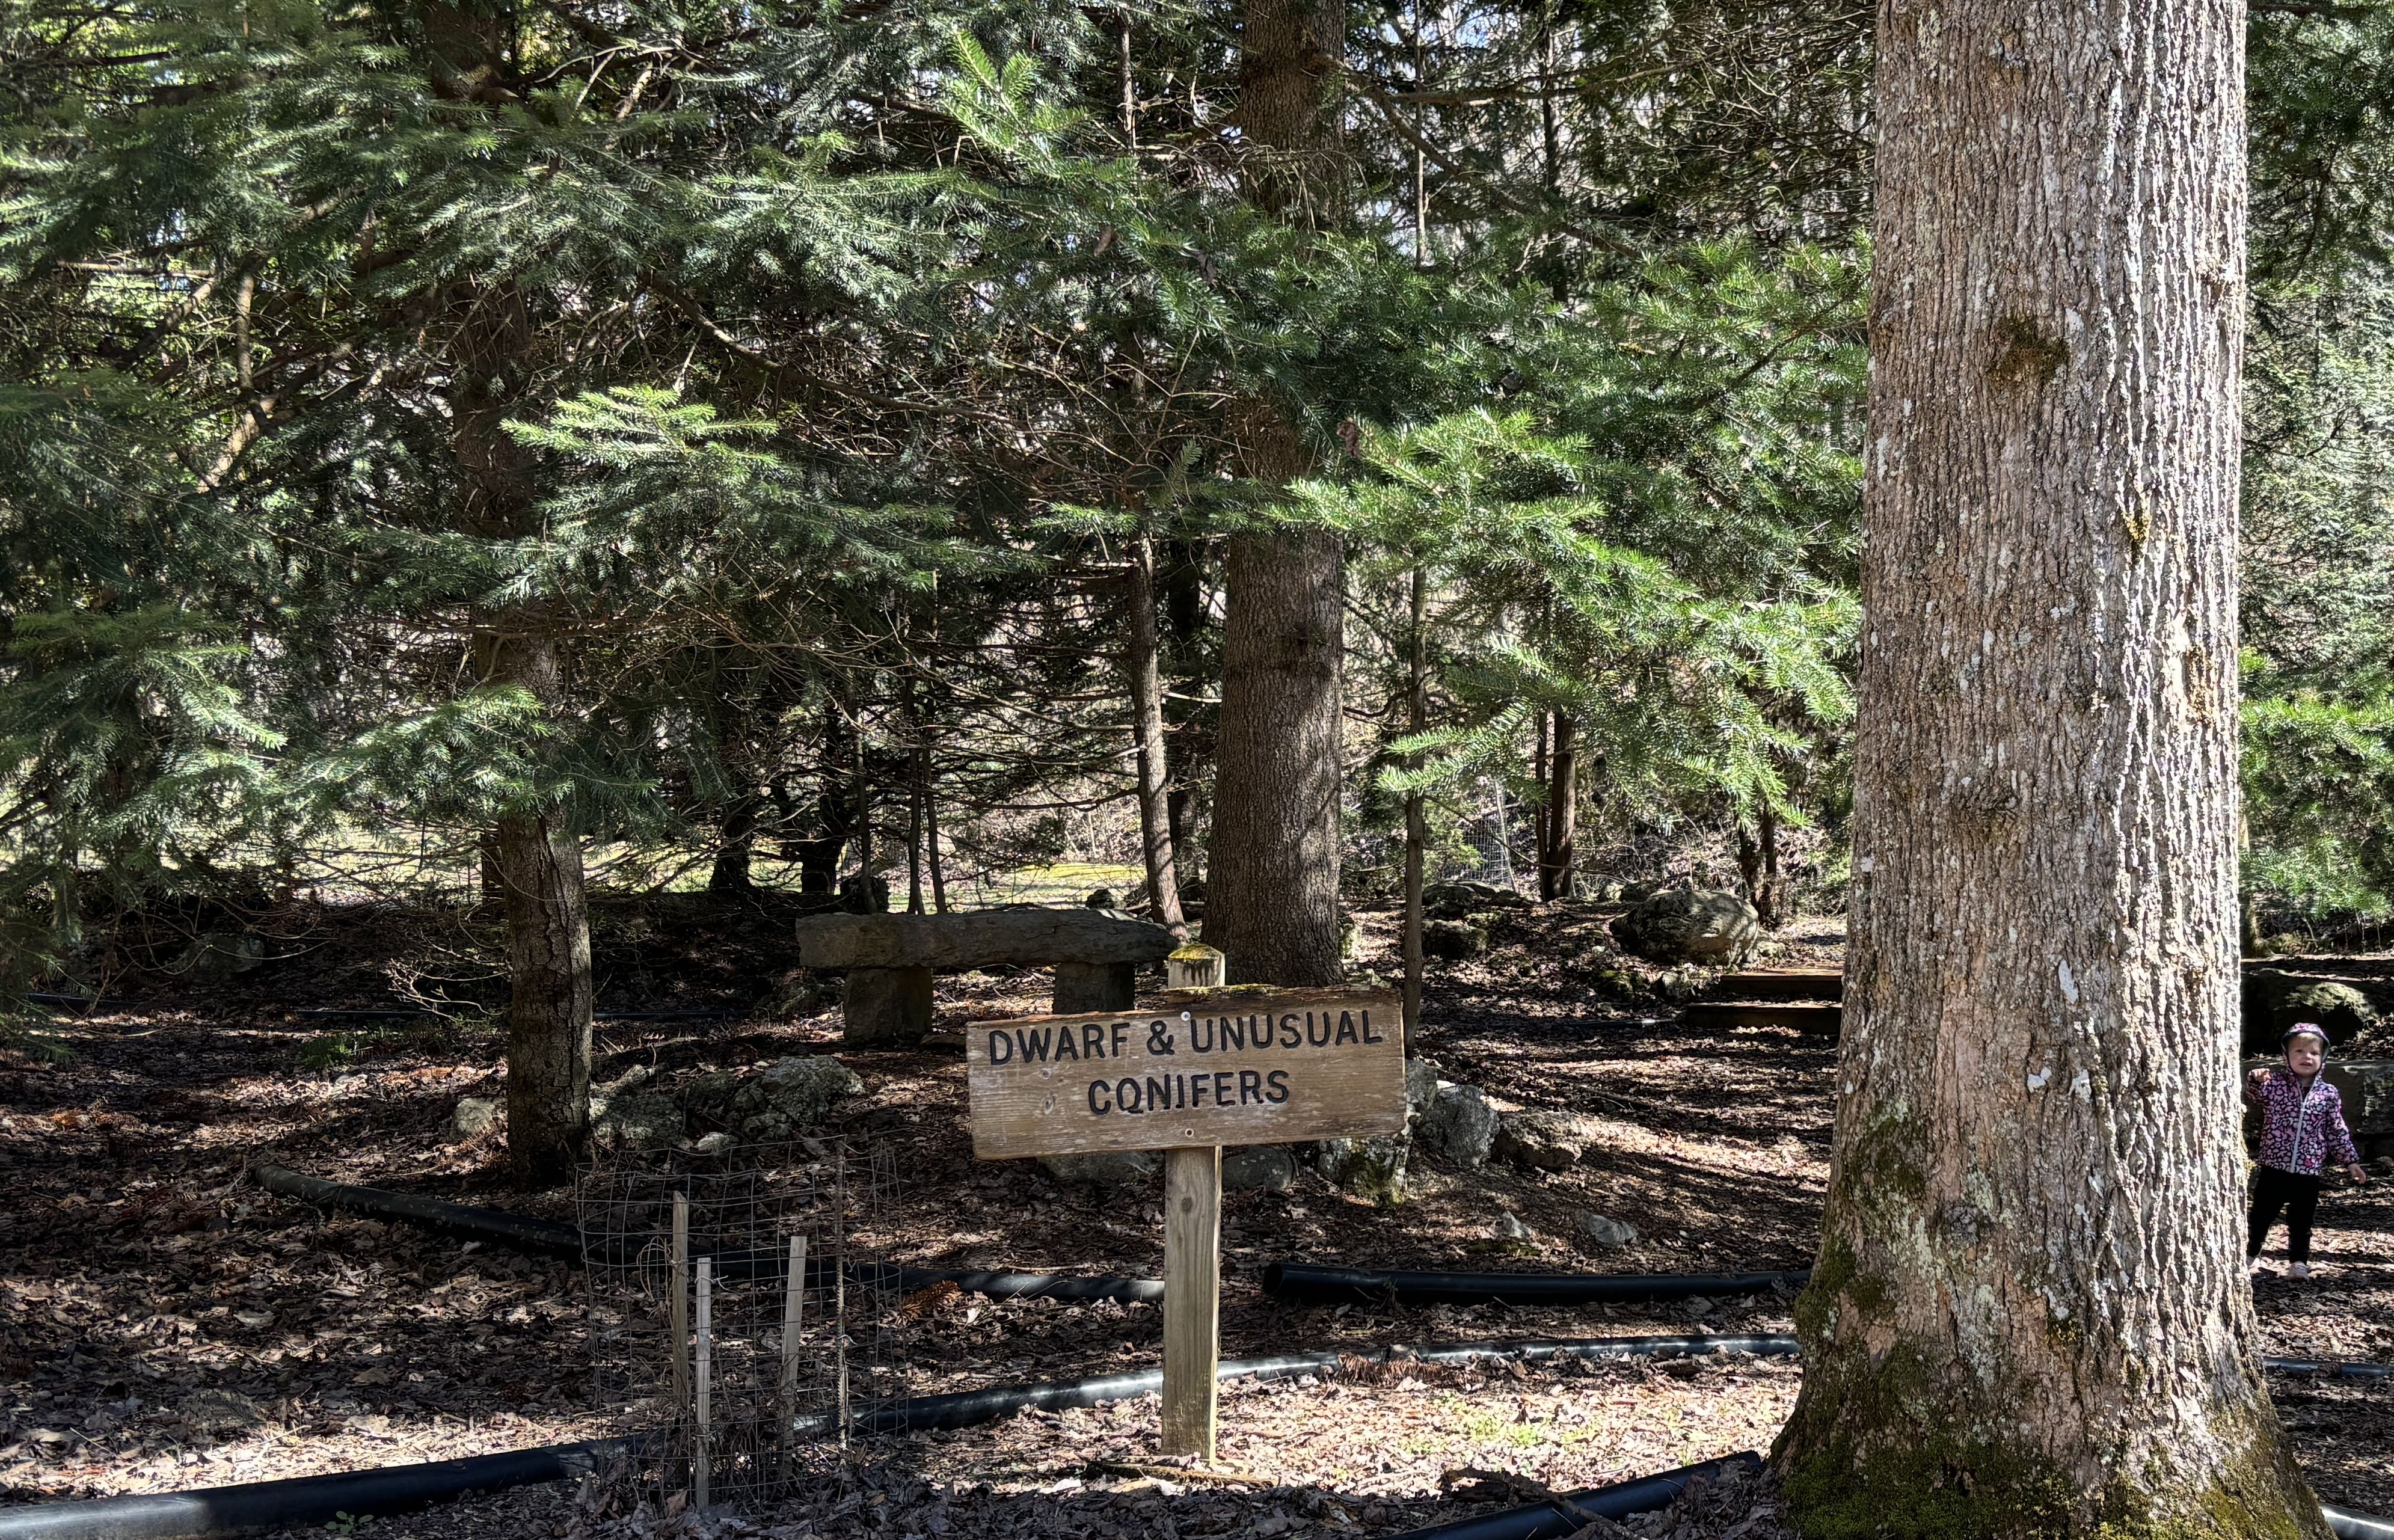
\includegraphics[keepaspectratio]{img/trail-05-figure-01.jpg}}

}

\caption{Photo credit to Katie and Joshua Rosenberg}

\end{figure}%

\subsection{Key Characteristics}\label{key-characteristics-5}

\begin{longtable}[]{@{}
  >{\raggedright\arraybackslash}p{(\linewidth - 2\tabcolsep) * \real{0.5745}}
  >{\raggedright\arraybackslash}p{(\linewidth - 2\tabcolsep) * \real{0.4255}}@{}}
\toprule\noalign{}
\begin{minipage}[b]{\linewidth}\raggedright
\textbf{Characteristic}
\end{minipage} & \begin{minipage}[b]{\linewidth}\raggedright
\textbf{Details}
\end{minipage} \\
\midrule\noalign{}
\endhead
\bottomrule\noalign{}
\endlastfoot
Time Estimate & 0.5 hours - 1 hour \\
Trail Distance (Miles) & 0.9 \\
Elevation Change & Gentle \\
Pets & Not Allowed \\
Parking Pass/Entrance Fee & Not Required \\
Restroom(s) & No \\
Best Ages & Toddlers and Little Kids \\
Strollers and Wheelchairs & Accessible \\
\end{longtable}

\pandocbounded{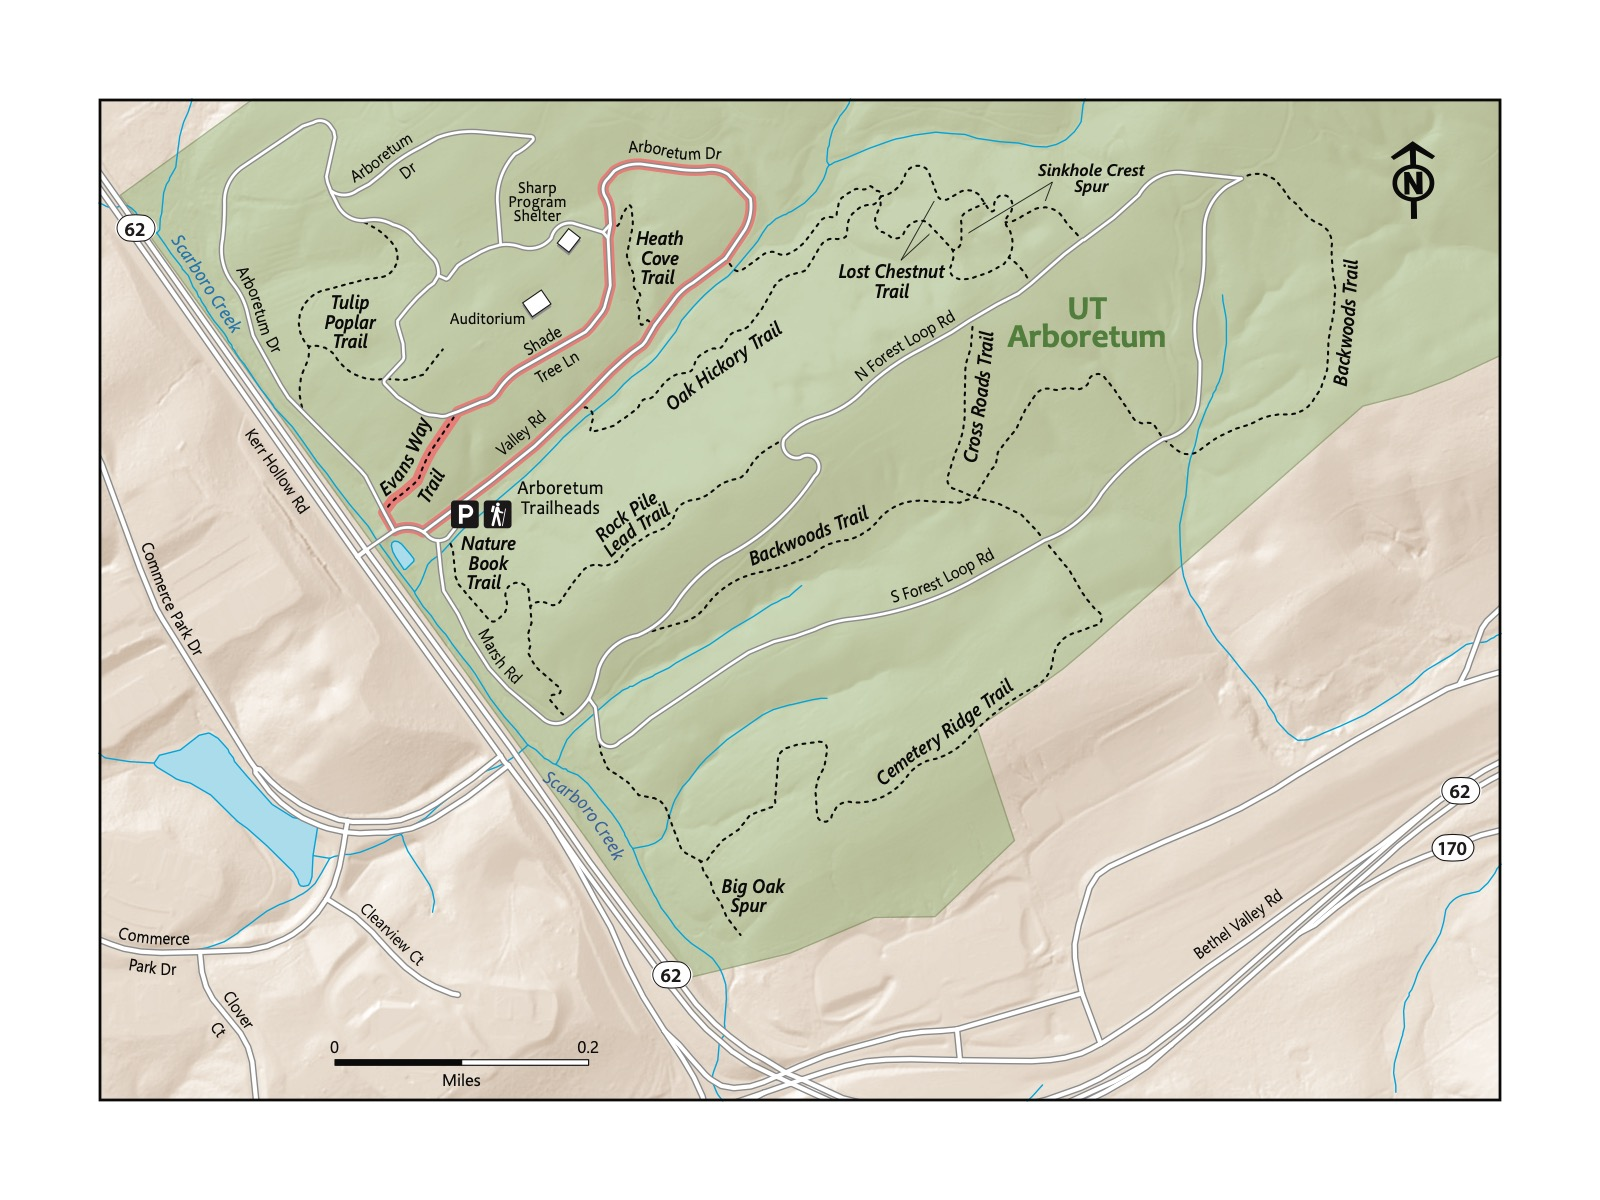
\includegraphics[keepaspectratio]{maps/trail-05-map.jpeg}}

\subsection{Directions to the
Trailhead}\label{directions-to-the-trailhead-4}

Trailhead Address: University of Tennessee Arboretum, 901 S Illinois
Ave, Oak Ridge, TN 37830

Trailhead GPS Coordinates: 35.99392, -84.21988

\subsection{Trail Description}\label{trail-description-4}

\begin{longtable}[]{@{}
  >{\raggedright\arraybackslash}p{(\linewidth - 2\tabcolsep) * \real{0.3521}}
  >{\raggedright\arraybackslash}p{(\linewidth - 2\tabcolsep) * \real{0.6479}}@{}}
\toprule\noalign{}
\begin{minipage}[b]{\linewidth}\raggedright
Distance from Start
\end{minipage} & \begin{minipage}[b]{\linewidth}\raggedright
Description
\end{minipage} \\
\midrule\noalign{}
\endhead
\bottomrule\noalign{}
\endlastfoot
0.0 & Walk along the paved road. \\
0.1 & Start of the Oak-Hickory Trail on the right. \\
0.2 & Start of the Heath Cove Trail on the left. This is a shortcut if
you're looking for one! \\
0.3 & Wind around, still on the road. \\
0.5 & Shelter on the right. \\
0.6 & Auditorium on the right. \\
0.7 & Leave the paved road for a short dirt path called Evans Way Trail.
Alternatively, turn around and head back on the paved path. \\
0.9 & Traihead. \\
\end{longtable}

\pandocbounded{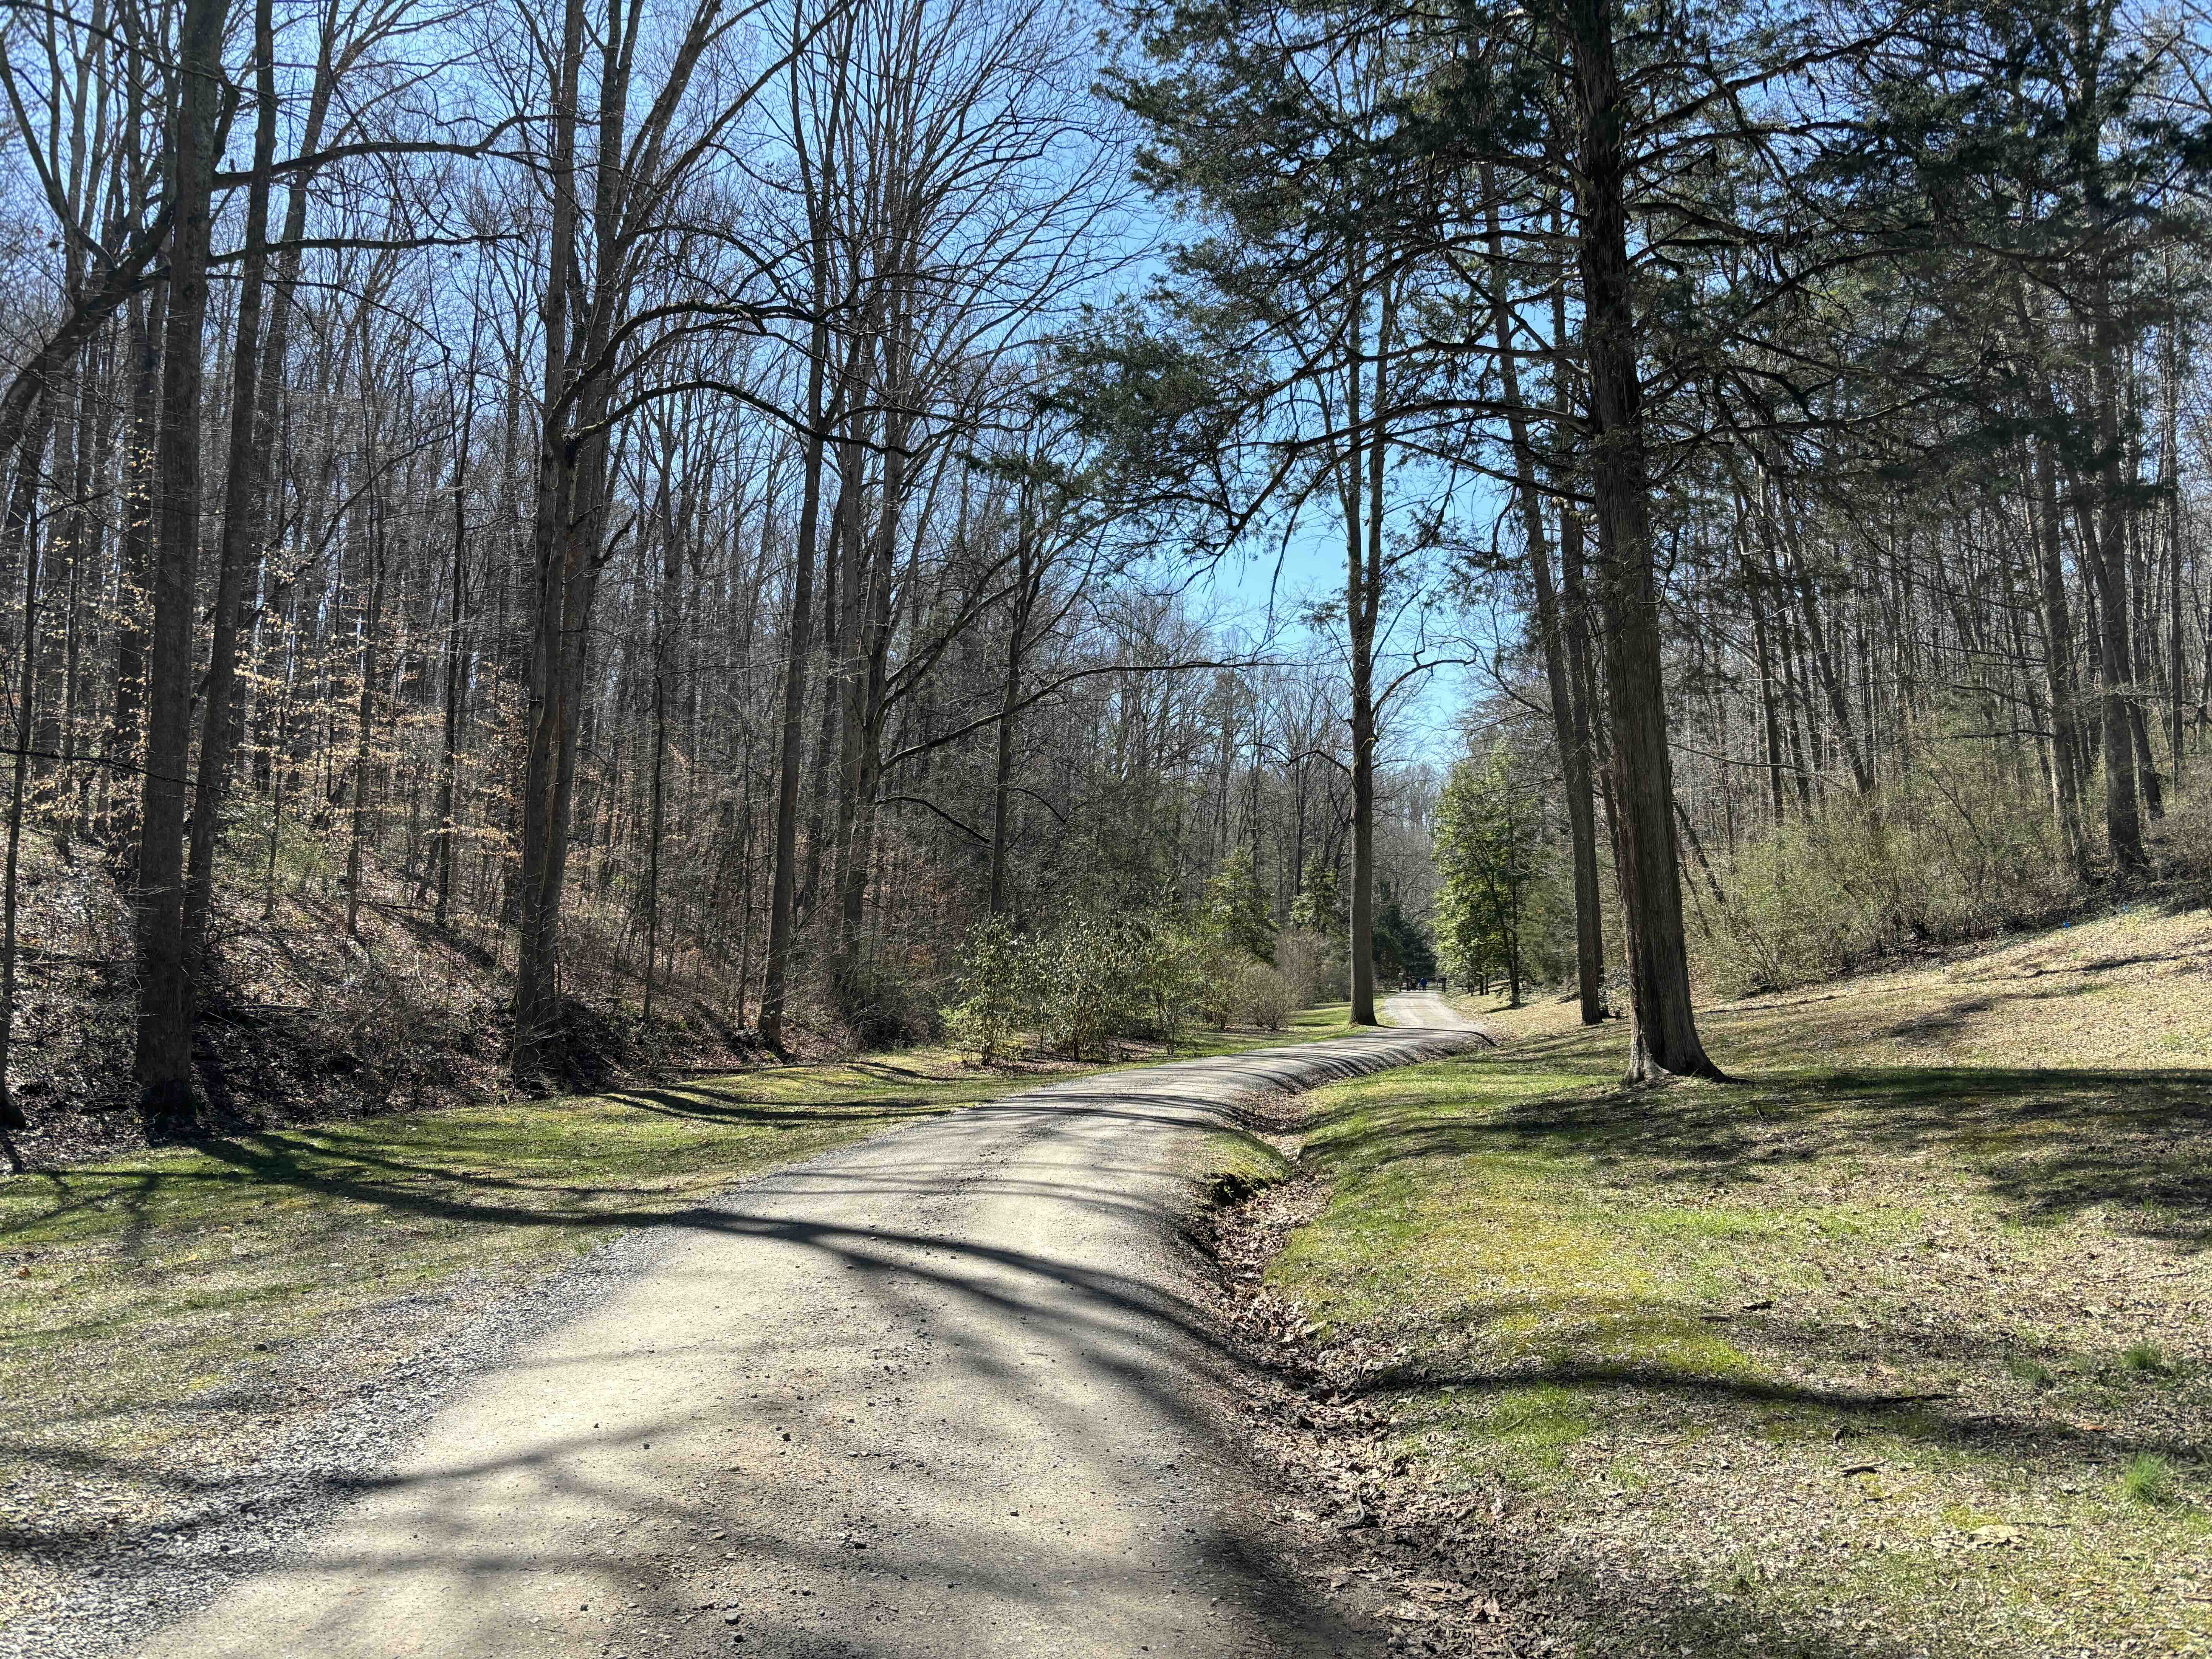
\includegraphics[keepaspectratio]{img/trail-05-figure-02.jpg}}

\subsection{Nearby}\label{nearby-4}

\begin{itemize}
\tightlist
\item
  \textbf{Explore some of the many other trails nearby.} The trail we
  featured meanders through a very small section of a large, diverse
  park. The Nature Book Trail is a great trail to add on to your hike.
  There are many others; check out the map at the UT Arboretum website
  (\url{https://utarboretum.tennessee.edu/}) to learn more.
\item
  \textbf{Bring the balance bikes and kids' bikes and stop by Haw Ridge
  and its kids' pump track.} Nearby Haw Ridge Park features the Dirtlab
  Mountain Bike Skill Park, a great spot for kids riding balance bikes
  and pedal bikes to hone their skills and build confidence!
\end{itemize}

\chapter{Trail 6: Knox-Blount
Greenway}\label{trail-6-knox-blount-greenway}

\subsection{Overview}\label{overview-6}

Another hike that is very close to Knoxville's city center, the
Knox-Blount Greenway, is a fun, easier outing for little walkers,
bikers, and for parents pushing little ones in strollers. Paved
throughout, this trail offers a glimpse of the surprising beauty of the
Tennessee River so close to the city. Our description features a route
that heads to the north, toward the city, and then back to the trail
from the research park further south, before returning to the start.
Look for blue herons and other birds along the side of the river; you
might see a Bald Eagle! While beautiful, there is limited shade here, so
factor the weather in before setting out to this destination! This will
be a fun hike for a gaggle of kids looking to toddle or run wild!

\begin{figure}[H]

{\centering \pandocbounded{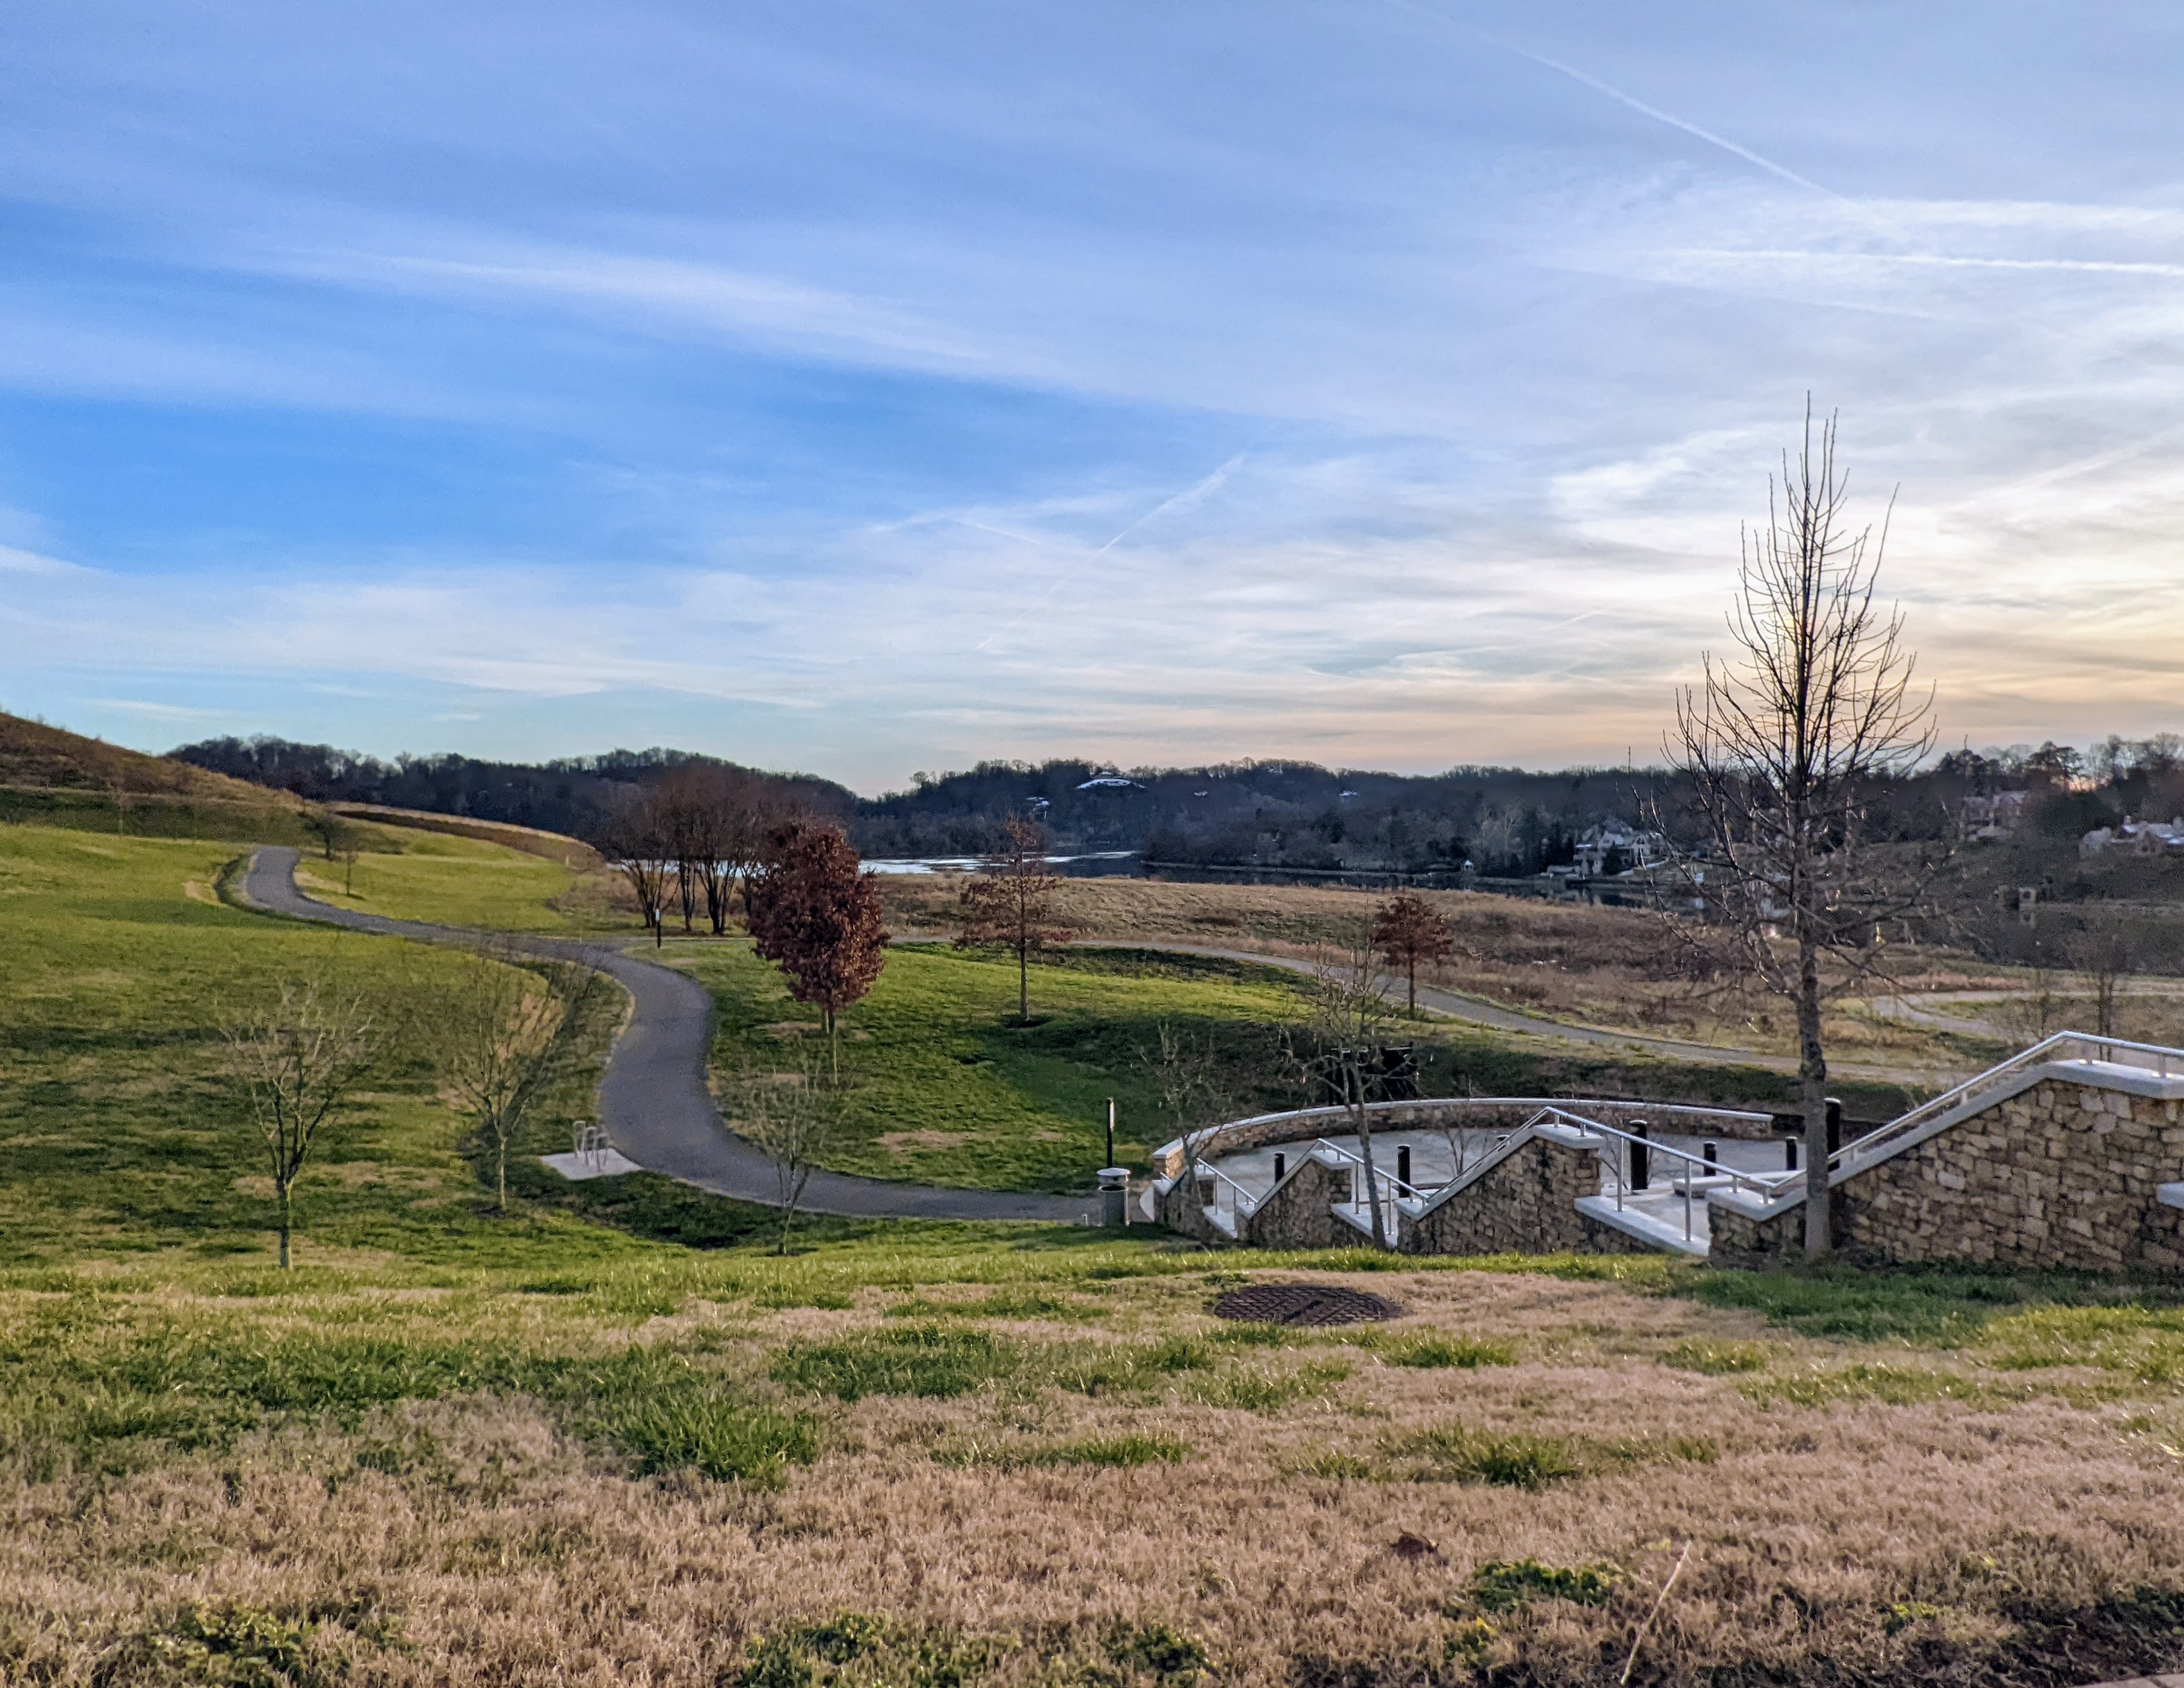
\includegraphics[keepaspectratio]{img/trail-06-figure-01.jpg}}

}

\caption{Photo credit to Katie and Joshua Rosenberg}

\end{figure}%

\subsection{Key Characteristics}\label{key-characteristics-6}

\begin{longtable}[]{@{}
  >{\raggedright\arraybackslash}p{(\linewidth - 2\tabcolsep) * \real{0.5294}}
  >{\raggedright\arraybackslash}p{(\linewidth - 2\tabcolsep) * \real{0.4706}}@{}}
\toprule\noalign{}
\begin{minipage}[b]{\linewidth}\raggedright
\textbf{Characteristic}
\end{minipage} & \begin{minipage}[b]{\linewidth}\raggedright
\textbf{Details}
\end{minipage} \\
\midrule\noalign{}
\endhead
\bottomrule\noalign{}
\endlastfoot
Time Estimate & 45 minutes - 1.5 hours \\
Trail Distance (Miles) & 2.3 \\
Elevation Change & Gentle \\
Pets & Allowed on leash \\
Parking Pass/Entrance Fee & Not Required \\
Restroom(s) & No \\
Best Ages & Toddlers and Little Kids \\
Strollers and Wheelchairs & Accessible \\
\end{longtable}

\pandocbounded{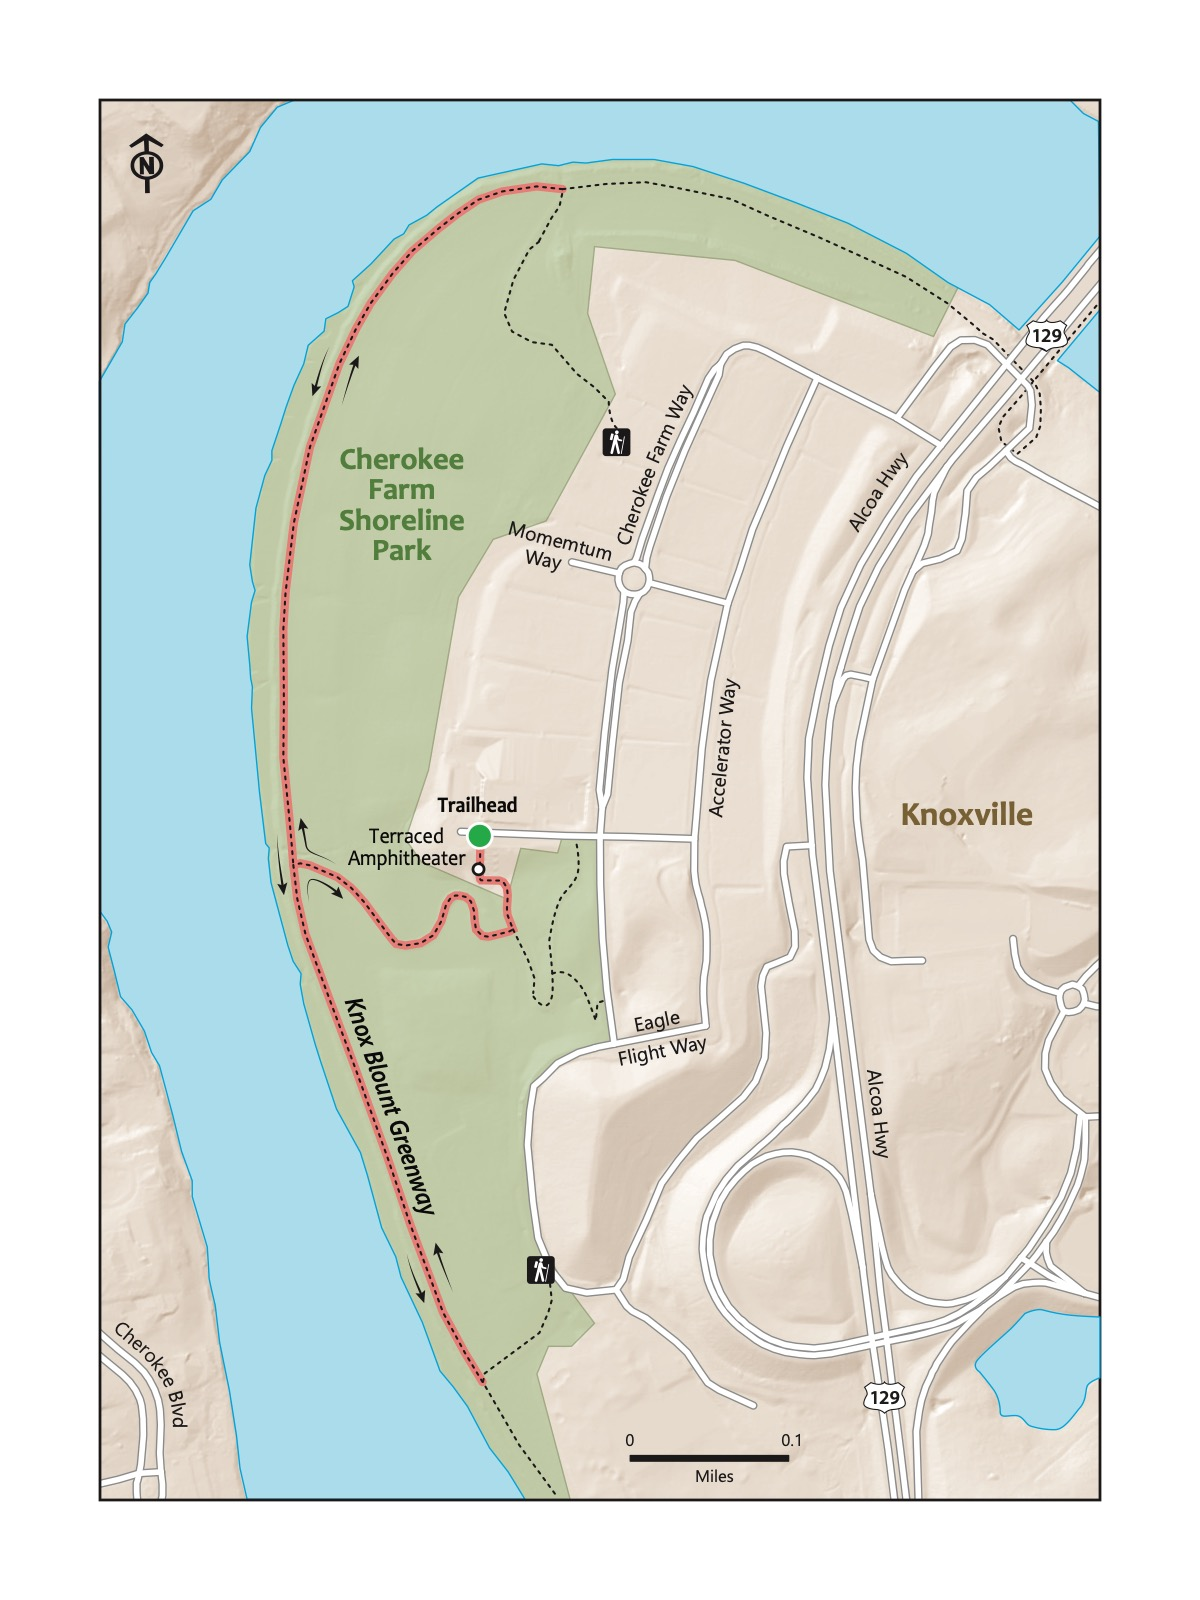
\includegraphics[keepaspectratio]{maps/trail-06-map.jpeg}}

\subsection{Directions to the
Trailhead}\label{directions-to-the-trailhead-5}

Trailhead Address: University of Tennessee Research Park at Cherokee
Farm, 2641 Osprey Vista Way, Knoxville, TN 37920

Trailhead GPS Coordinates: 35.94191, -83.95270

Park in the lot at the above address. If helpful, the building next to
the lot is the IAM Electron Microscopy Facility. The start of the trail
is at the top of a terraced amphitheater---conveniently, one that's easy
to walk down.

\begin{tcolorbox}[enhanced jigsaw, colback=white, colframe=quarto-callout-note-color-frame, breakable, opacityback=0, toprule=.15mm, bottomrule=.15mm, rightrule=.15mm, left=2mm, leftrule=.75mm, arc=.35mm]
\begin{minipage}[t]{5.5mm}
\textcolor{quarto-callout-note-color}{\faInfo}
\end{minipage}%
\begin{minipage}[t]{\textwidth - 5.5mm}

\vspace{-3mm}\textbf{Bald Eagle}\vspace{3mm}

Common along local rivers, including the river beside this hike---the
Tennessee River. You may even spot a nesting pair on nearby Looney
Island.

\end{minipage}%
\end{tcolorbox}

\subsection{Trail Description}\label{trail-description-5}

\begin{longtable}[]{@{}
  >{\raggedright\arraybackslash}p{(\linewidth - 2\tabcolsep) * \real{0.2361}}
  >{\raggedright\arraybackslash}p{(\linewidth - 2\tabcolsep) * \real{0.7639}}@{}}
\toprule\noalign{}
\begin{minipage}[b]{\linewidth}\raggedright
Distance from Start
\end{minipage} & \begin{minipage}[b]{\linewidth}\raggedright
Description
\end{minipage} \\
\midrule\noalign{}
\endhead
\bottomrule\noalign{}
\endlastfoot
0.0 & Walk down the terraced amphitheater. \\
0.1 & Begin to descend down a gradual hill. \\
0.3 & Reach the river and the Knox-Blount Greenway trail proper. Our
route turns right, but you can explore in either direction! \\
0.35 & Follow the greenway along the river. The meadows to the right are
usually mowed; kids may like to cruise through them! \\
0.8 & Our preferred route turns around at the intersection of the
greenway and a spur trail. Of course, you can continue further if you
like. Head back the other direction \\
1.3 & Pass the trail from the amphitheater you took earlier, continuing
along the river. \\
1.65 & Turn around at the intersection of another spur trail. \\
2.0 & Meet back up with the trail to the amphitheater. \\
2.3 & Traihead. \\
\end{longtable}

\subsection{Nearby}\label{nearby-5}

\begin{itemize}
\tightlist
\item
  \textbf{Take time to visit the UT Gardens.} The nearby UT Gardens
  (2621 Morgan Circle, Knoxville, TN 37996) is a great spot for a
  meander through beautiful gardens. Be sure to check out the Children's
  Garden featuring grassy mounds and ample play structures!
\item
  \textbf{Bike the greenways!} While we featured the Knox-Blount
  Greenway as a hike, it's also a fun bike ride for young bikers.
\end{itemize}

\chapter{Trail 7: Sequoyah Park}\label{trail-7-sequoyah-park}

\subsection{Overview}\label{overview-7}

This is another gem among Knoxville city parks, nestled in the heart of
the the city in a neighborhood. The trail starts at a large parking area
near the restroom building and walks towards the river. It follows the
river past open fields, trees, and bushes which playfully beckon for
kids not to explore! The trail cuts up toward the greenway and hikes
past Indian burial mounds and the historic homes along the path before
returning to the start. In mild weather, it is a fantastic spot to hang
up a hammock, fish, have a picnic, or toss a frisbee or a football. This
outing is ideal for kids of all walking ages, and alternate ways to
access the greenway make it easy to create a shorter loop.

\begin{figure}[H]

{\centering \pandocbounded{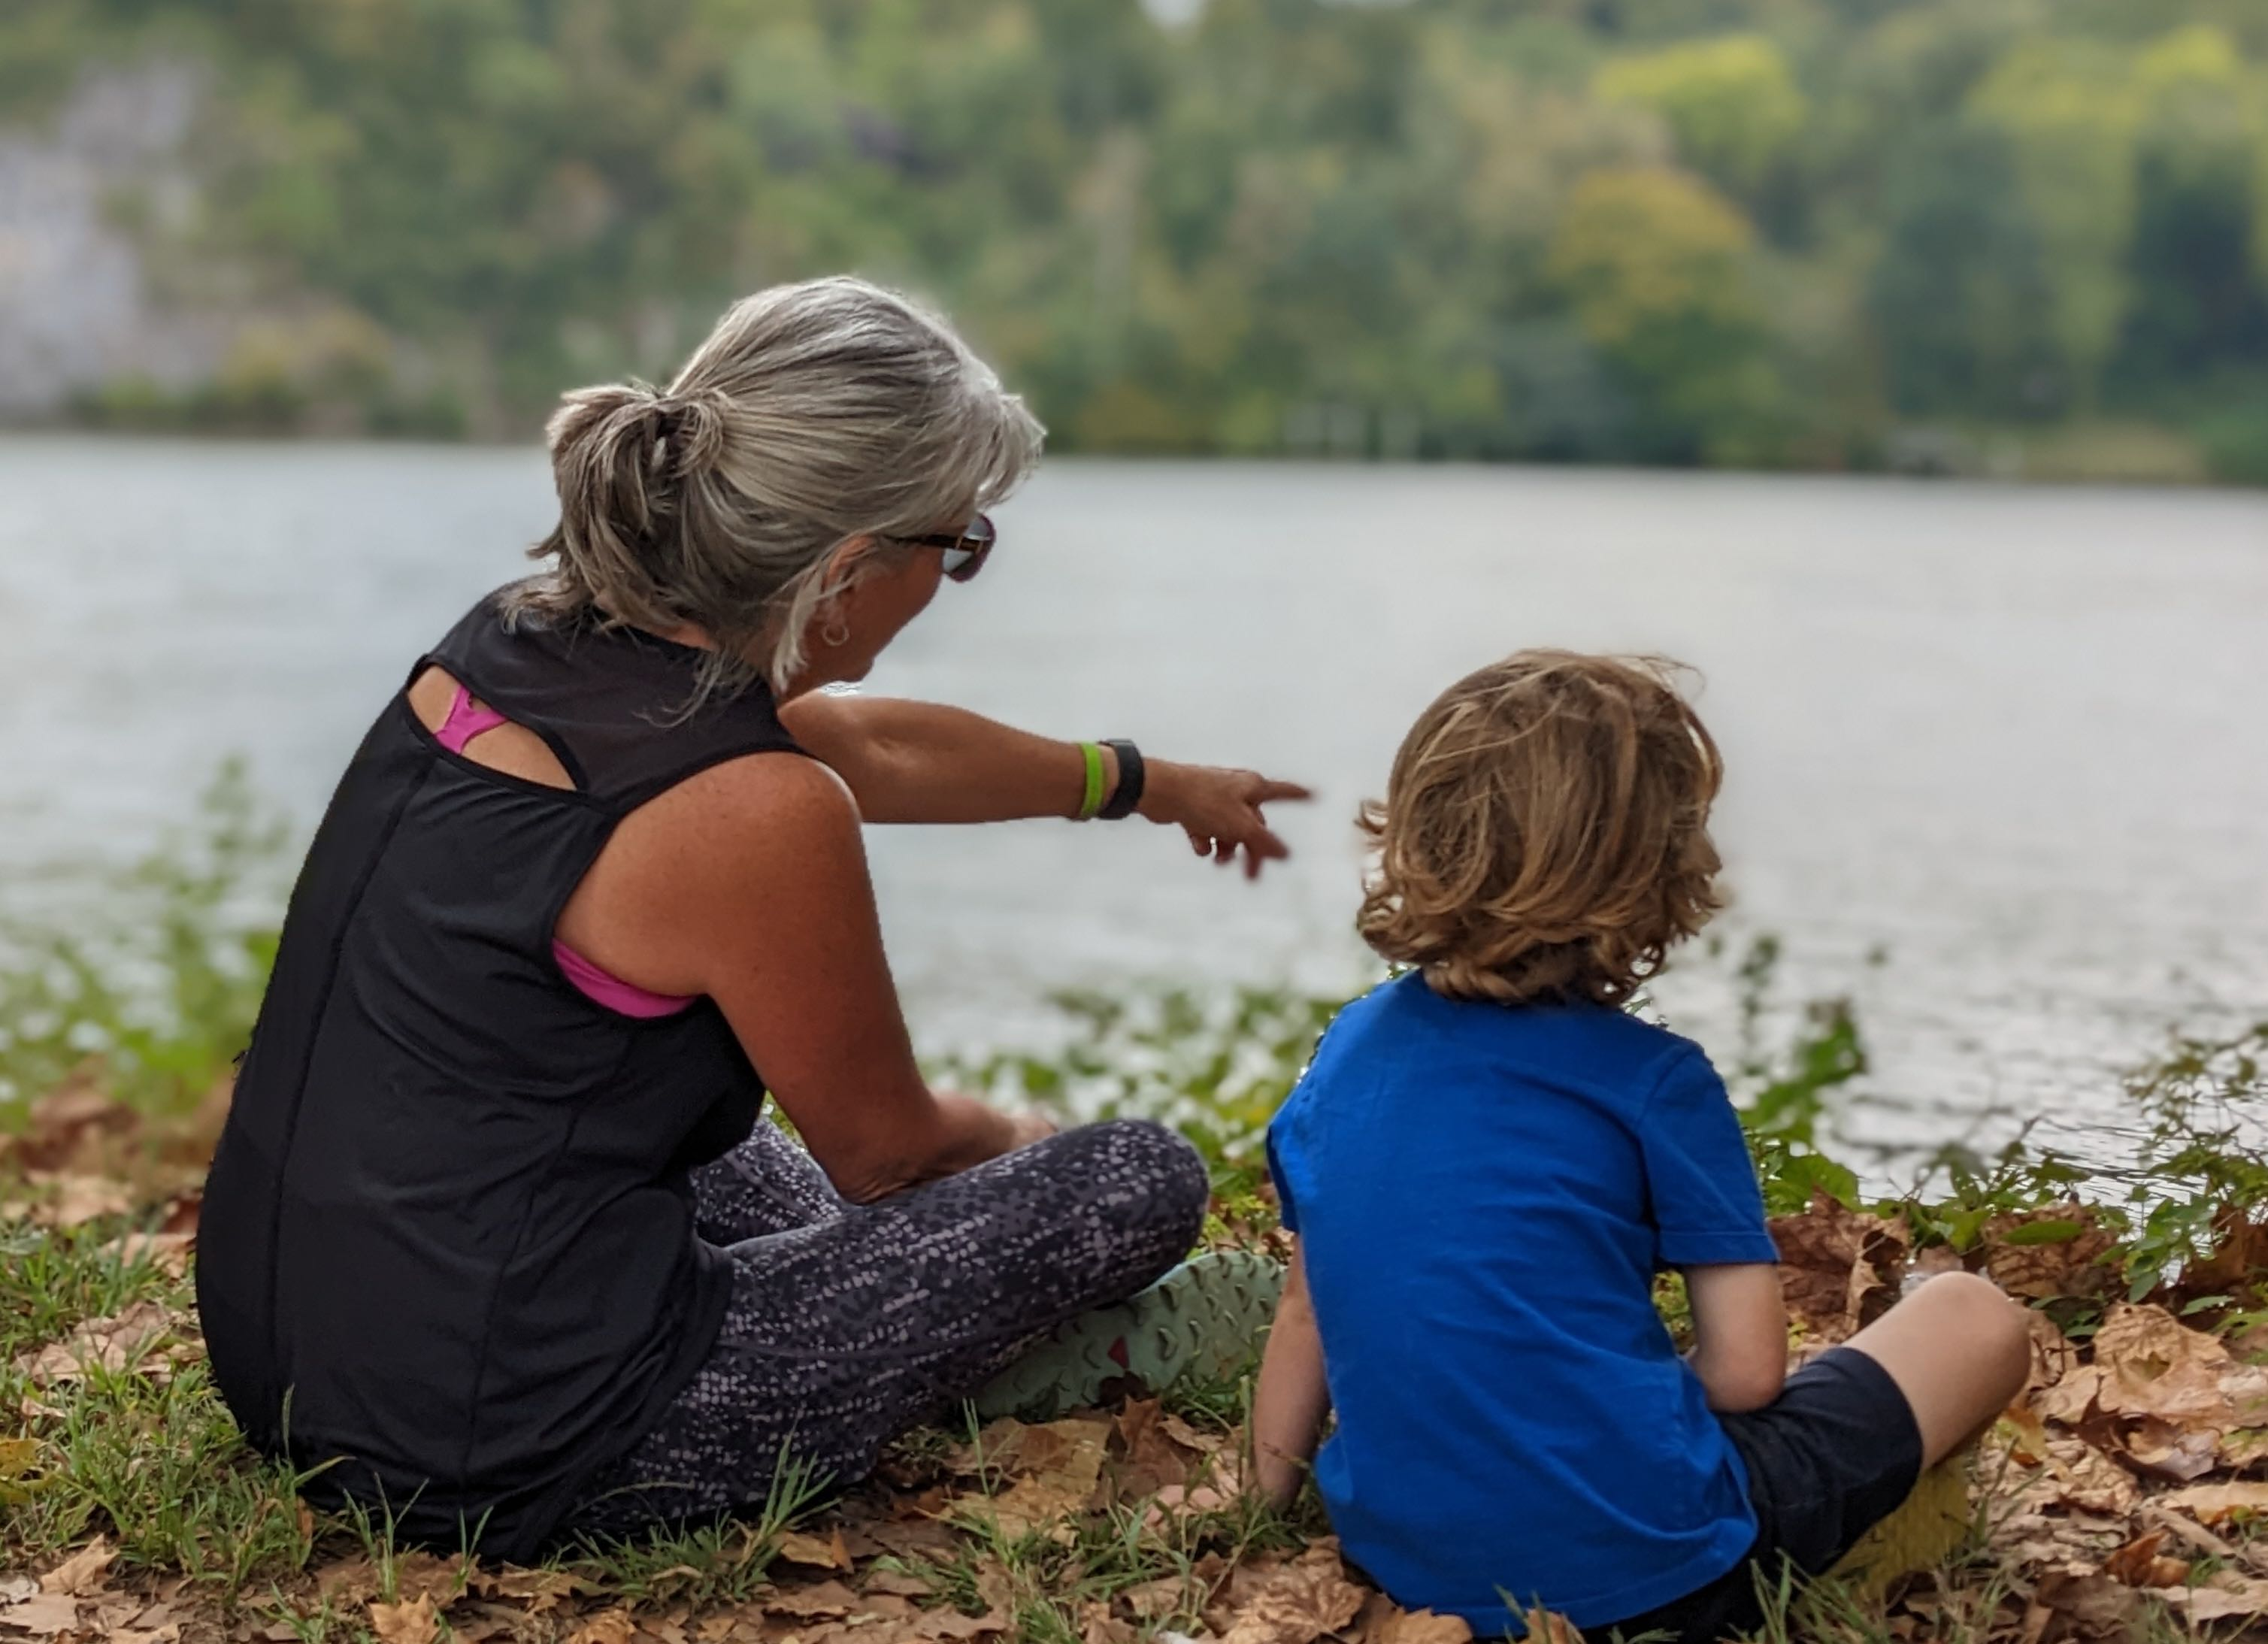
\includegraphics[keepaspectratio]{img/trail-07-figure-01.jpg}}

}

\caption{Photo credit to Katie and Joshua Rosenberg}

\end{figure}%

\subsection{Key Characteristics}\label{key-characteristics-7}

\begin{longtable}[]{@{}ll@{}}
\toprule\noalign{}
\textbf{Characteristic} & \textbf{Details} \\
\midrule\noalign{}
\endhead
\bottomrule\noalign{}
\endlastfoot
Time Estimate & 1 hour - 2 hours \\
Trail Distance (Miles) & 2.1 \\
Elevation Change & Flat \\
Pets & Allowed on leash \\
Parking Pass/Entrance Fee & Not Required \\
Restroom(s) & Yes \\
Best Ages & Toddlers and Little Kids \\
Strollers and Wheelchairs & Not accessible \\
\end{longtable}

\pandocbounded{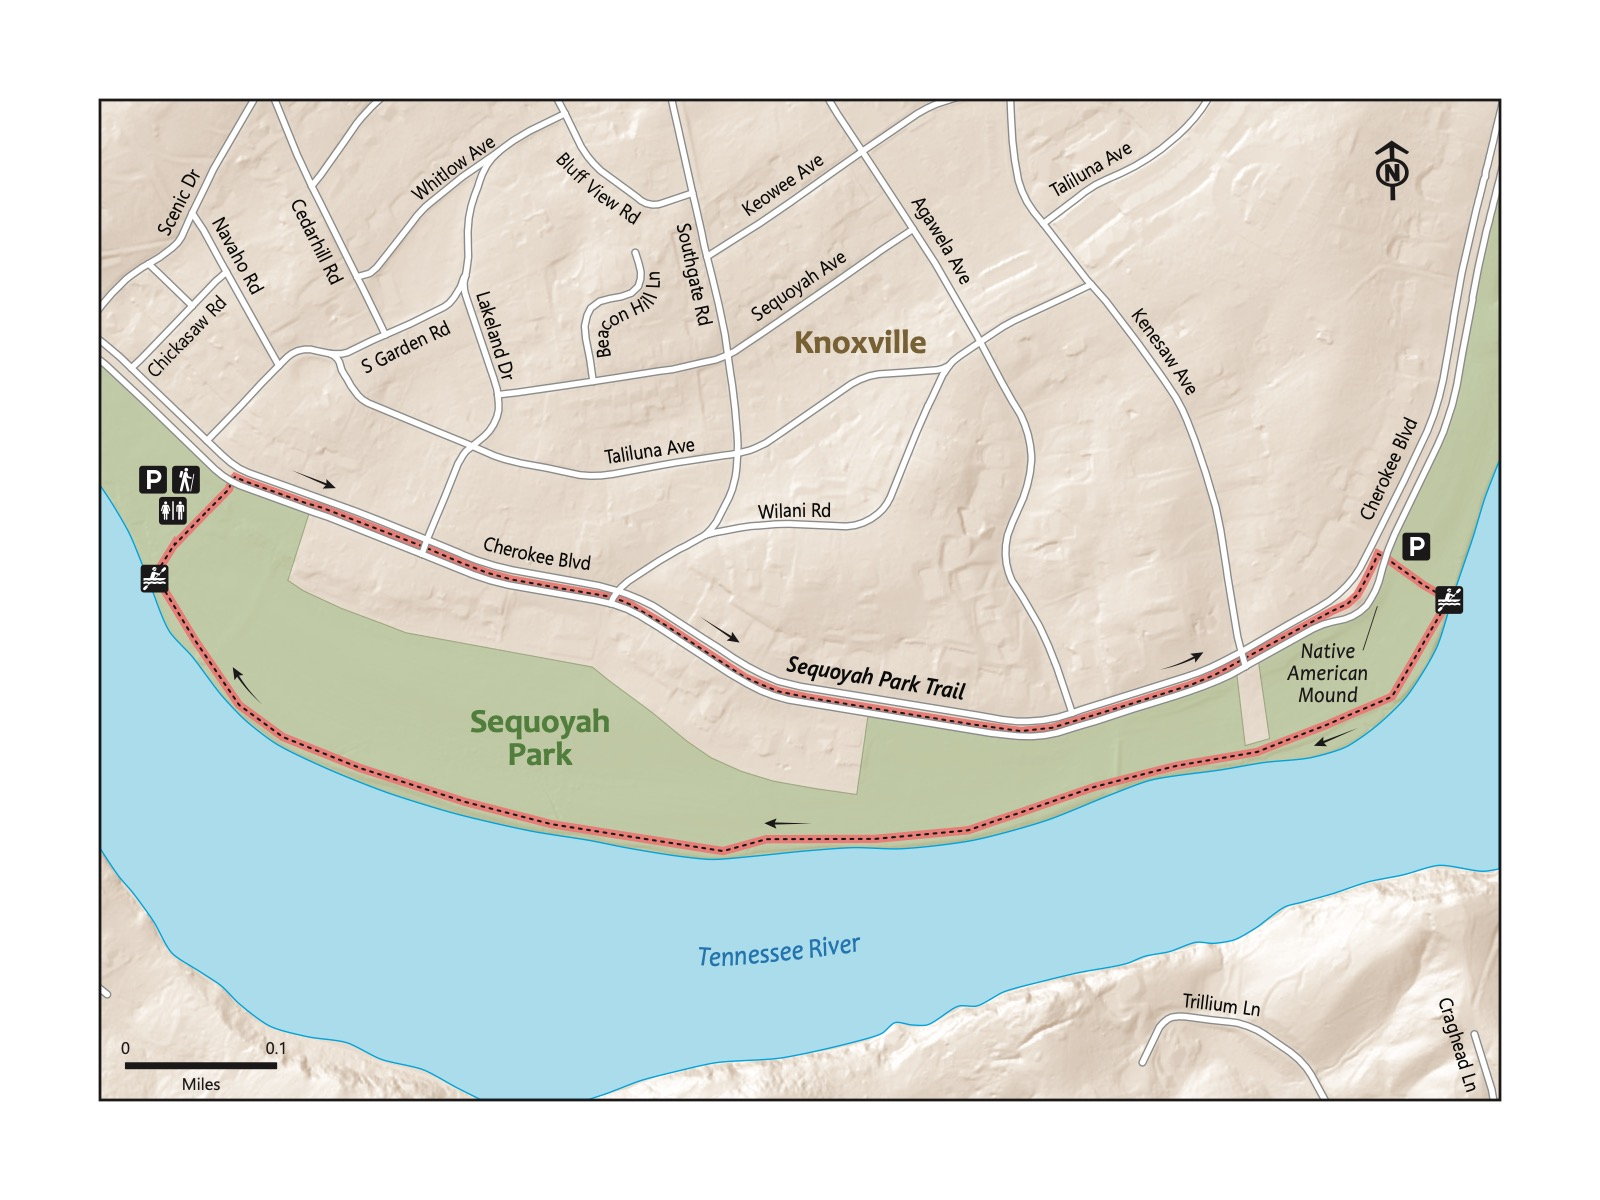
\includegraphics[keepaspectratio]{maps/trail-07-map.jpeg}}

\subsection{Directions to the
Trailhead}\label{directions-to-the-trailhead-6}

Trailhead Address: Sequoyah Park Restrooms, W2HG+M9, Knoxville, TN 37919

Trailhead GPS Coordinates: 35.92932, -83.97398

\begin{tcolorbox}[enhanced jigsaw, colback=white, colframe=quarto-callout-note-color-frame, breakable, opacityback=0, toprule=.15mm, bottomrule=.15mm, rightrule=.15mm, left=2mm, leftrule=.75mm, arc=.35mm]
\begin{minipage}[t]{5.5mm}
\textcolor{quarto-callout-note-color}{\faInfo}
\end{minipage}%
\begin{minipage}[t]{\textwidth - 5.5mm}

\vspace{-3mm}\textbf{Elm Tree}\vspace{3mm}

Trees characterized by an umbrella-shaped crown. The tree near the start
of this hike (surrounded by a wire enclosure to prevent cars from being
parked nearby) is known as a ``Champion'' of its kind -- the largest Elm
in Knoxville.

\end{minipage}%
\end{tcolorbox}

The above address takes you to the parking area next to restrooms that
serve as a landmark for this sprawling park. Please note that the
address uses a ``Plus'' code that only works with Google Maps because
the restrooms and trailhead don't have an assigned address. \%EXPLAIN
PLUS CODE\%

\subsection{Trail Description}\label{trail-description-6}

\begin{longtable}[]{@{}
  >{\raggedright\arraybackslash}p{(\linewidth - 2\tabcolsep) * \real{0.1321}}
  >{\raggedright\arraybackslash}p{(\linewidth - 2\tabcolsep) * \real{0.8679}}@{}}
\toprule\noalign{}
\begin{minipage}[b]{\linewidth}\raggedright
Distance from Start
\end{minipage} & \begin{minipage}[b]{\linewidth}\raggedright
Description
\end{minipage} \\
\midrule\noalign{}
\endhead
\bottomrule\noalign{}
\endlastfoot
0.0 & Walk southwest (toward the large, open part of the park) along the
river. \\
0.1 & Kayak and canoe put in spot on the right. \\
0.25 & Enter a wooded section. \\
0.4 & Bench. \\
0.65 & Distinctive, dome-shaded trees that kids can crawl into, between,
and through. \\
0.9 & Small rocky hill to walk over (you can walk around it on the
greenway, but kids may enjoy scrambling up it). \\
1.1 & Boat launch. Head up beside or through the parking lot to Sequoyah
Greenway in the center of Cherokee Blvd. Turn left onto the greenway. \\
1.2 & Native American mound. Note the historical marker. Walk along past
the homes on both sides of the greenway. \\
2.05 & Traihead. \\
\end{longtable}

\begin{tcolorbox}[enhanced jigsaw, colback=white, colframe=quarto-callout-note-color-frame, breakable, opacityback=0, toprule=.15mm, bottomrule=.15mm, rightrule=.15mm, left=2mm, leftrule=.75mm, arc=.35mm]
\begin{minipage}[t]{5.5mm}
\textcolor{quarto-callout-note-color}{\faInfo}
\end{minipage}%
\begin{minipage}[t]{\textwidth - 5.5mm}

\vspace{-3mm}\textbf{Native American Mounds}\vspace{3mm}

These earthen mounds are found in many places along the Mississippi
River and its tributaries---like the Tennessee River. Nobody is
completely sure why they were built, but some believe they served as
gathering spots or markers to return to time and again. The mound here
may date back as early as the 1400s, likely created by one of the Native
Nations with ancestral ties to the Knoxville region.

\end{minipage}%
\end{tcolorbox}

\begin{figure}[H]

{\centering \pandocbounded{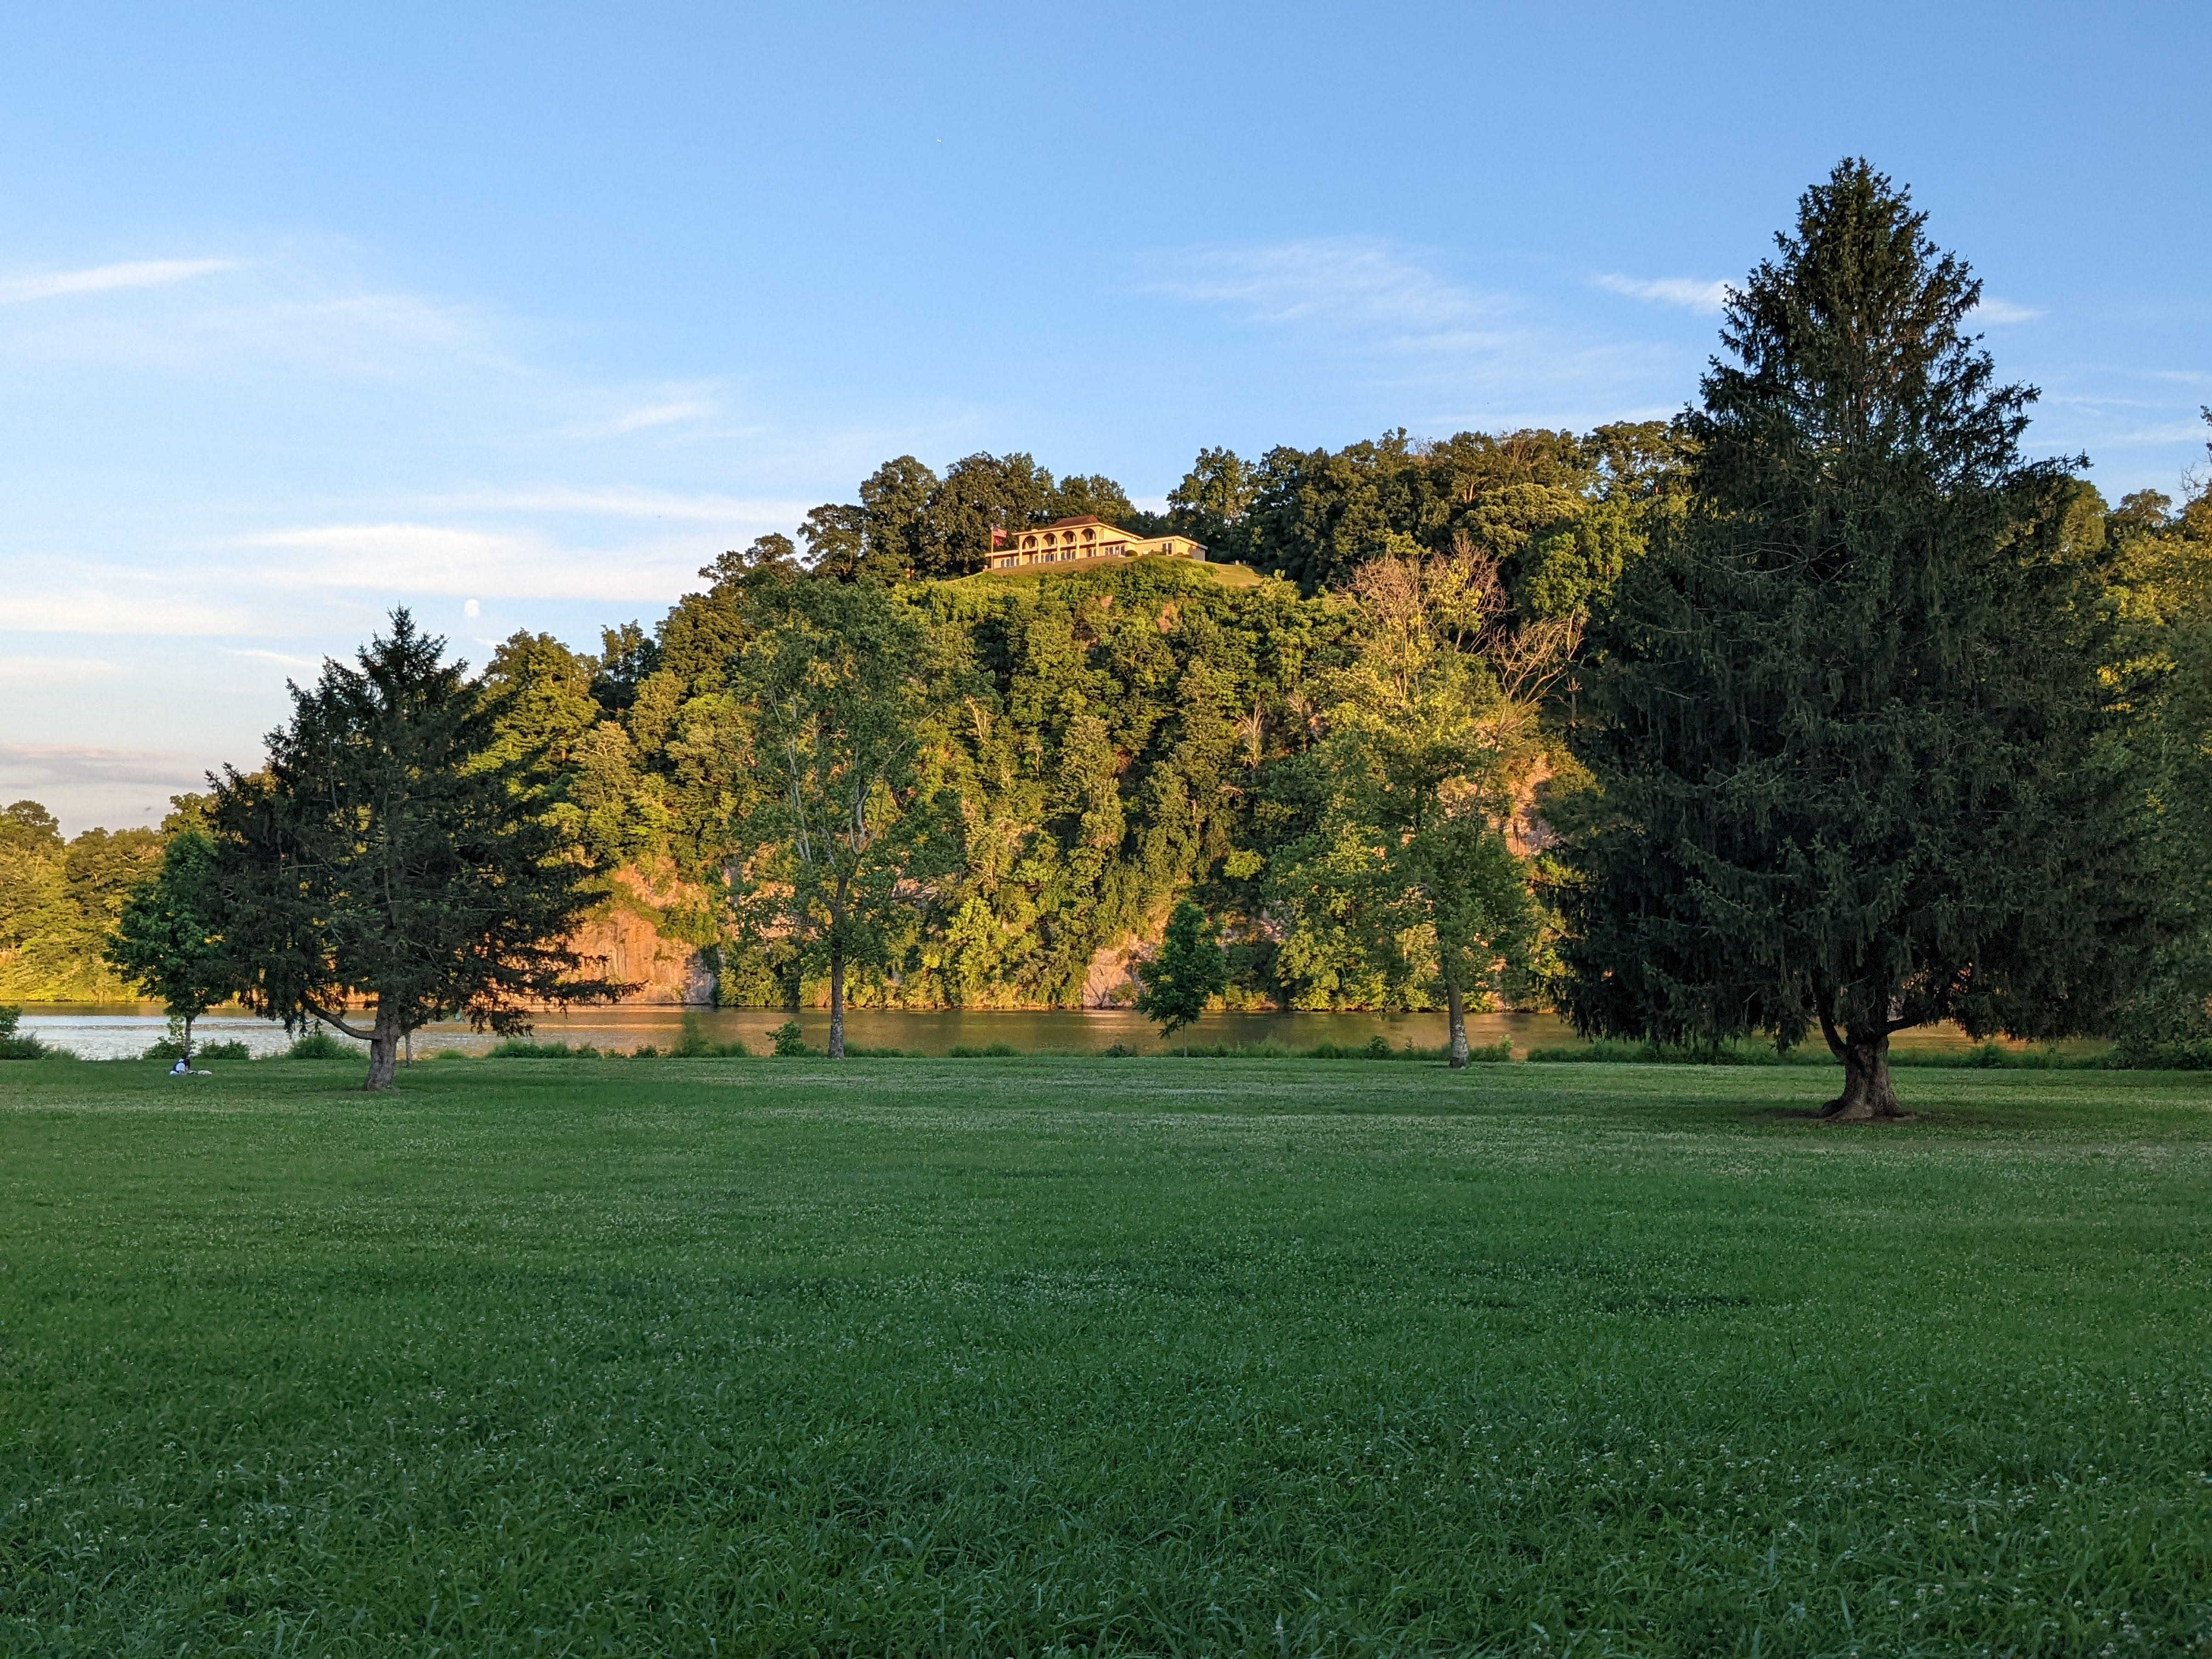
\includegraphics[keepaspectratio]{img/trail-07-figure-02.jpg}}

}

\caption{Photo credit to Katie and Joshua Rosenberg}

\end{figure}%

\subsection{Nearby}\label{nearby-6}

\begin{itemize}
\tightlist
\item
  \textbf{Grab a coffee, baked good, or breakfast!} Nearby Treetop
  Coffee Shop (1206 Kenesaw Ave, Knoxville, TN 37919) and The Plaid
  Apron restaurant (1210 Kenesaw Ave, Knoxville, TN 37919) next door are
  great places to stop by. Check their hours of operation before
  visiting!
\item
  \textbf{Explore a bit more of the neighborhood!} Nearby Whitlow Park
  (4228 Whitlow Ave SW, Knoxville, TN 37919) features a small but fun
  playground, nice tennis courts, and a basketball court.
\end{itemize}

\chapter{Trail 8: Ijams Crag}\label{trail-8-ijams-crag}

\subsection{Overview}\label{overview-8}

This trail is a nice introduction to the area of Ijams that is centered
around Mead's Quarry, which Ijams refers to as the Quarryside area. The
hike begins at the quarry and winds up a smooth then rocky trail. The
overlook is for Ijams Crag, a popular outdoor rock climbing area. We
love having a snack at the shade of the pine trees at the overlook.
After winding back to the start, be sure to explore one of the two
excellent nature play areas nearby or take a side trail back to extend
the trip. This area offers something for all ages, but the hike itself
is best suited to young hikers who are able navigate steeper, rocky
terrain. Younger hikers will need assistance.

\begin{figure}[H]

{\centering \pandocbounded{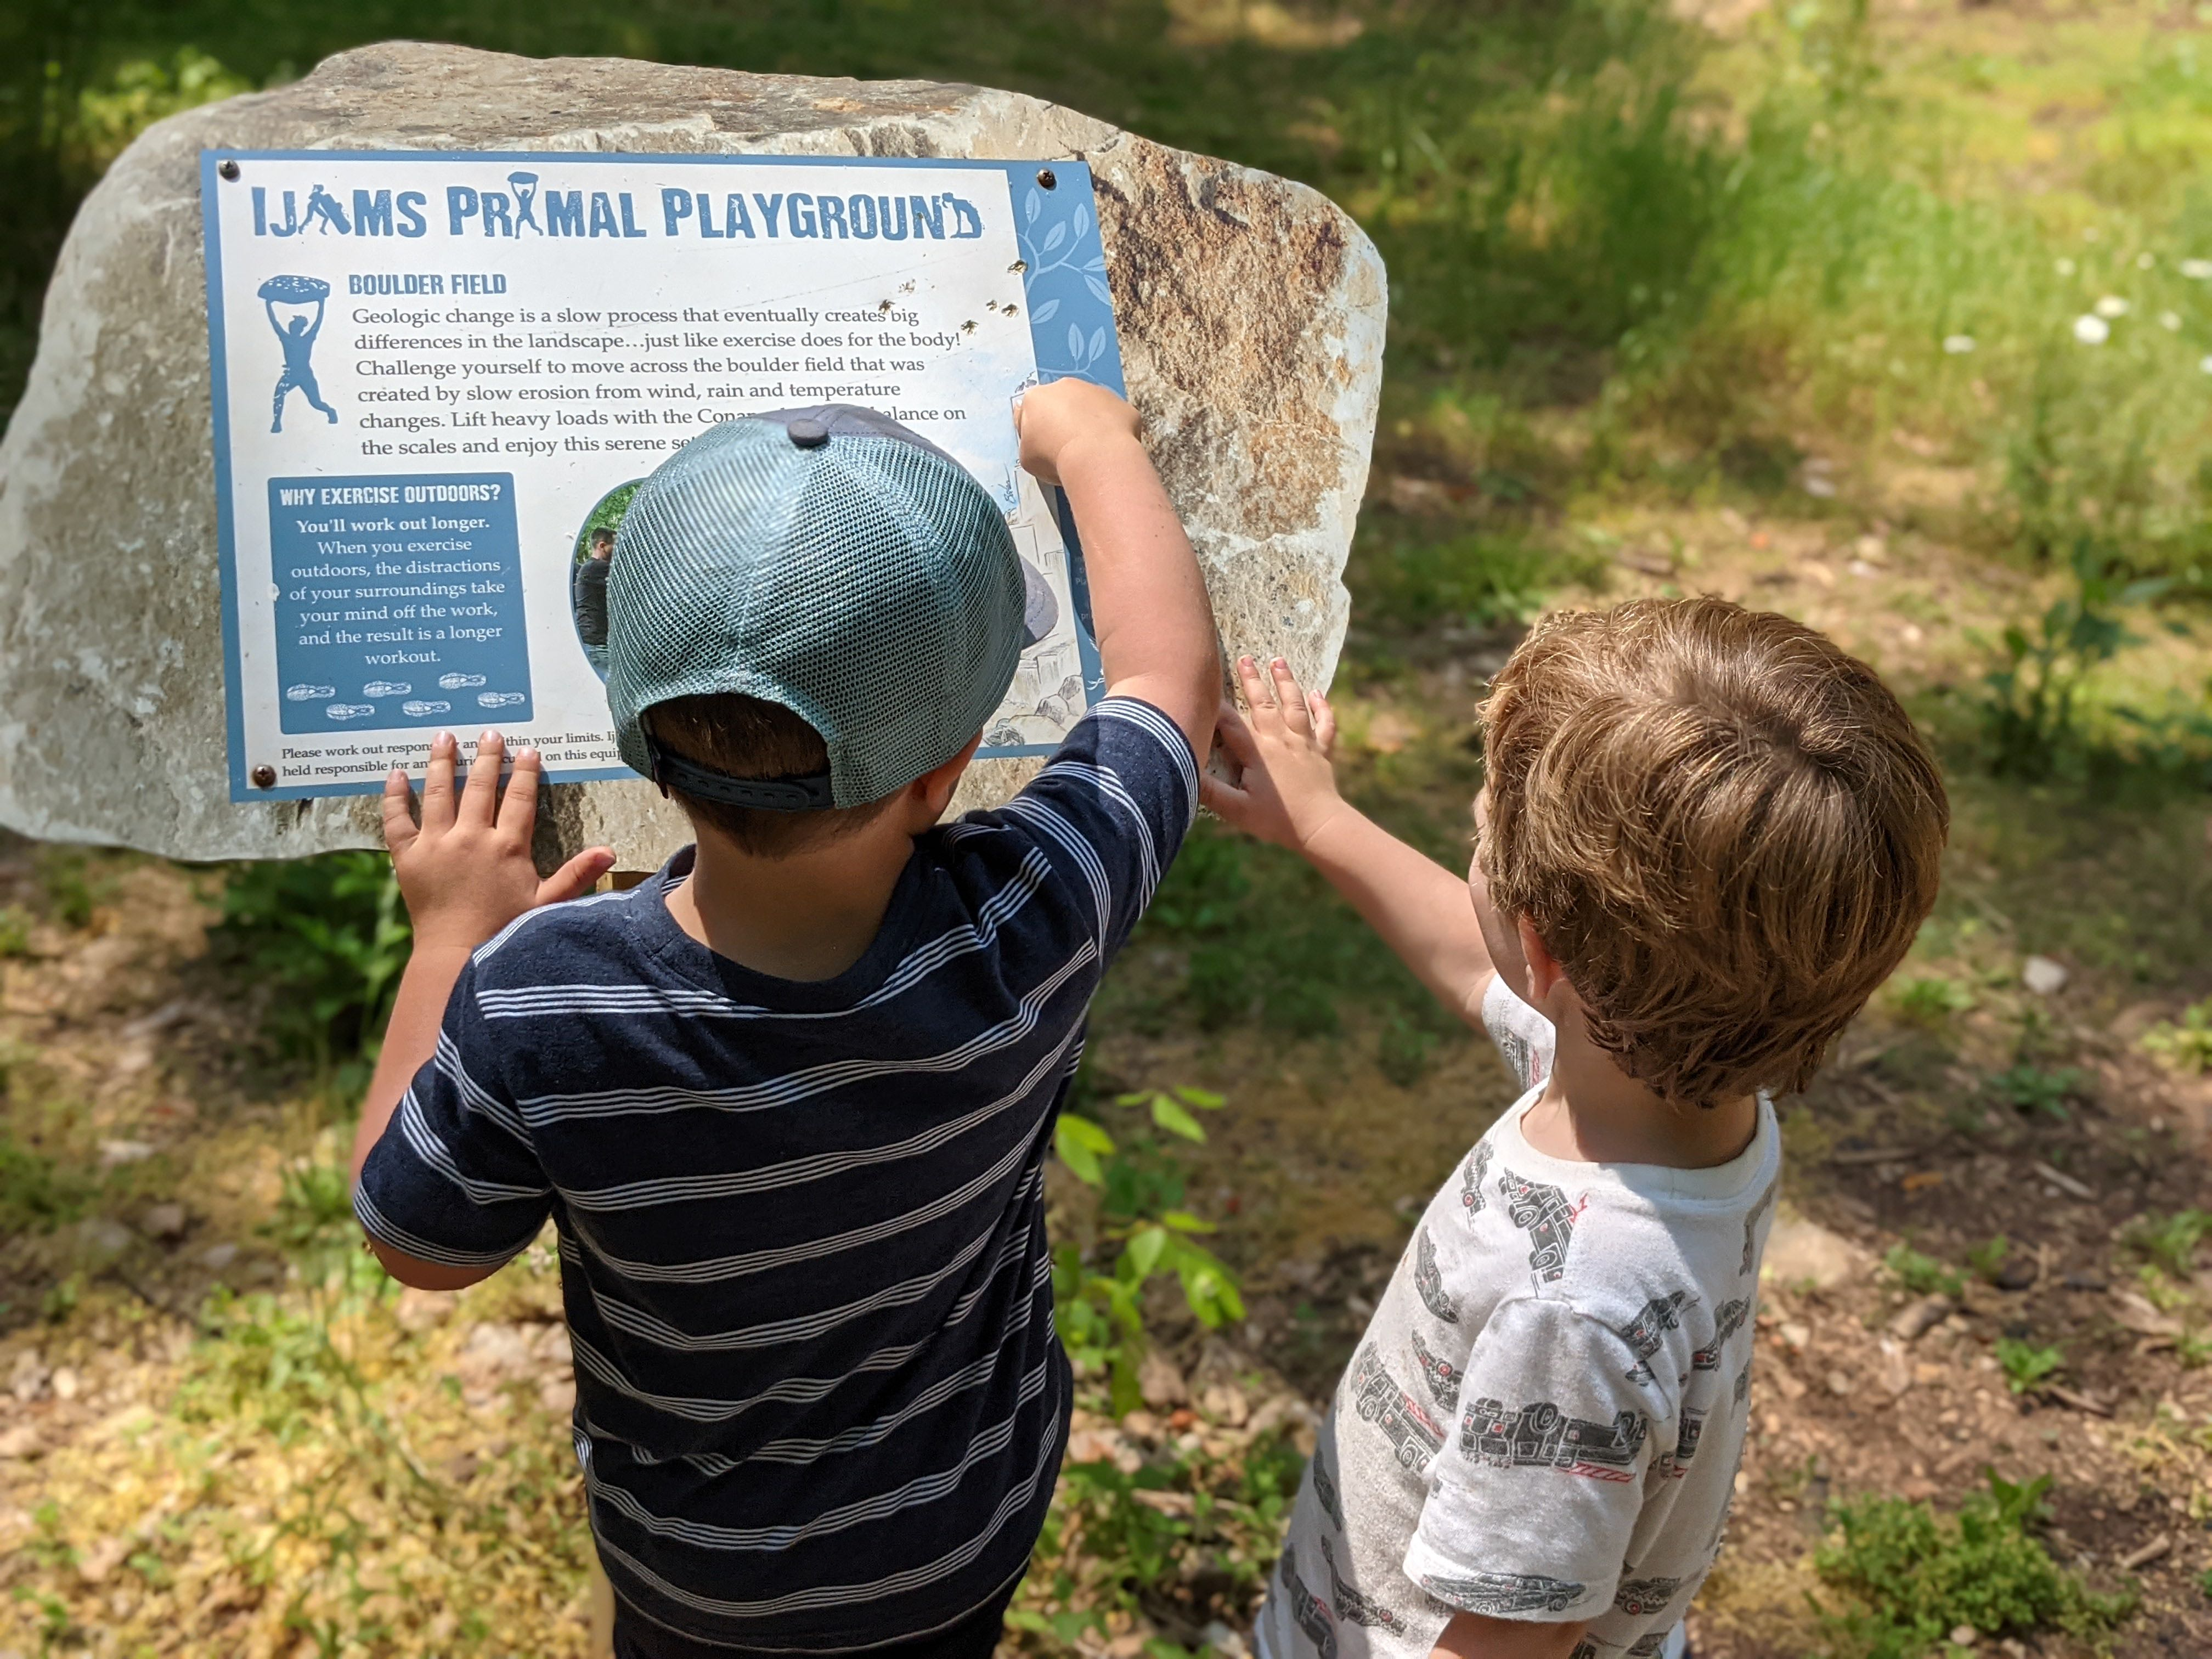
\includegraphics[keepaspectratio]{img/trail-08-figure-01.jpg}}

}

\caption{Photo credit to Katie and Joshua Rosenberg}

\end{figure}%

\subsection{Key Characteristics}\label{key-characteristics-8}

\begin{longtable}[]{@{}
  >{\raggedright\arraybackslash}p{(\linewidth - 2\tabcolsep) * \real{0.5294}}
  >{\raggedright\arraybackslash}p{(\linewidth - 2\tabcolsep) * \real{0.4706}}@{}}
\toprule\noalign{}
\begin{minipage}[b]{\linewidth}\raggedright
\textbf{Characteristic}
\end{minipage} & \begin{minipage}[b]{\linewidth}\raggedright
\textbf{Details}
\end{minipage} \\
\midrule\noalign{}
\endhead
\bottomrule\noalign{}
\endlastfoot
Time Estimate & 45 minutes - 1.5 hours \\
Trail Distance (Miles) & 1.5 \\
Elevation Change & Moderate \\
Pets & Allowed on leash \\
Parking Pass/Entrance Fee & Not Required \\
Restroom(s) & Yes \\
Best Ages & Little Kids and Big Kids \\
Strollers and Wheelchairs & Not accessible \\
\end{longtable}

\pandocbounded{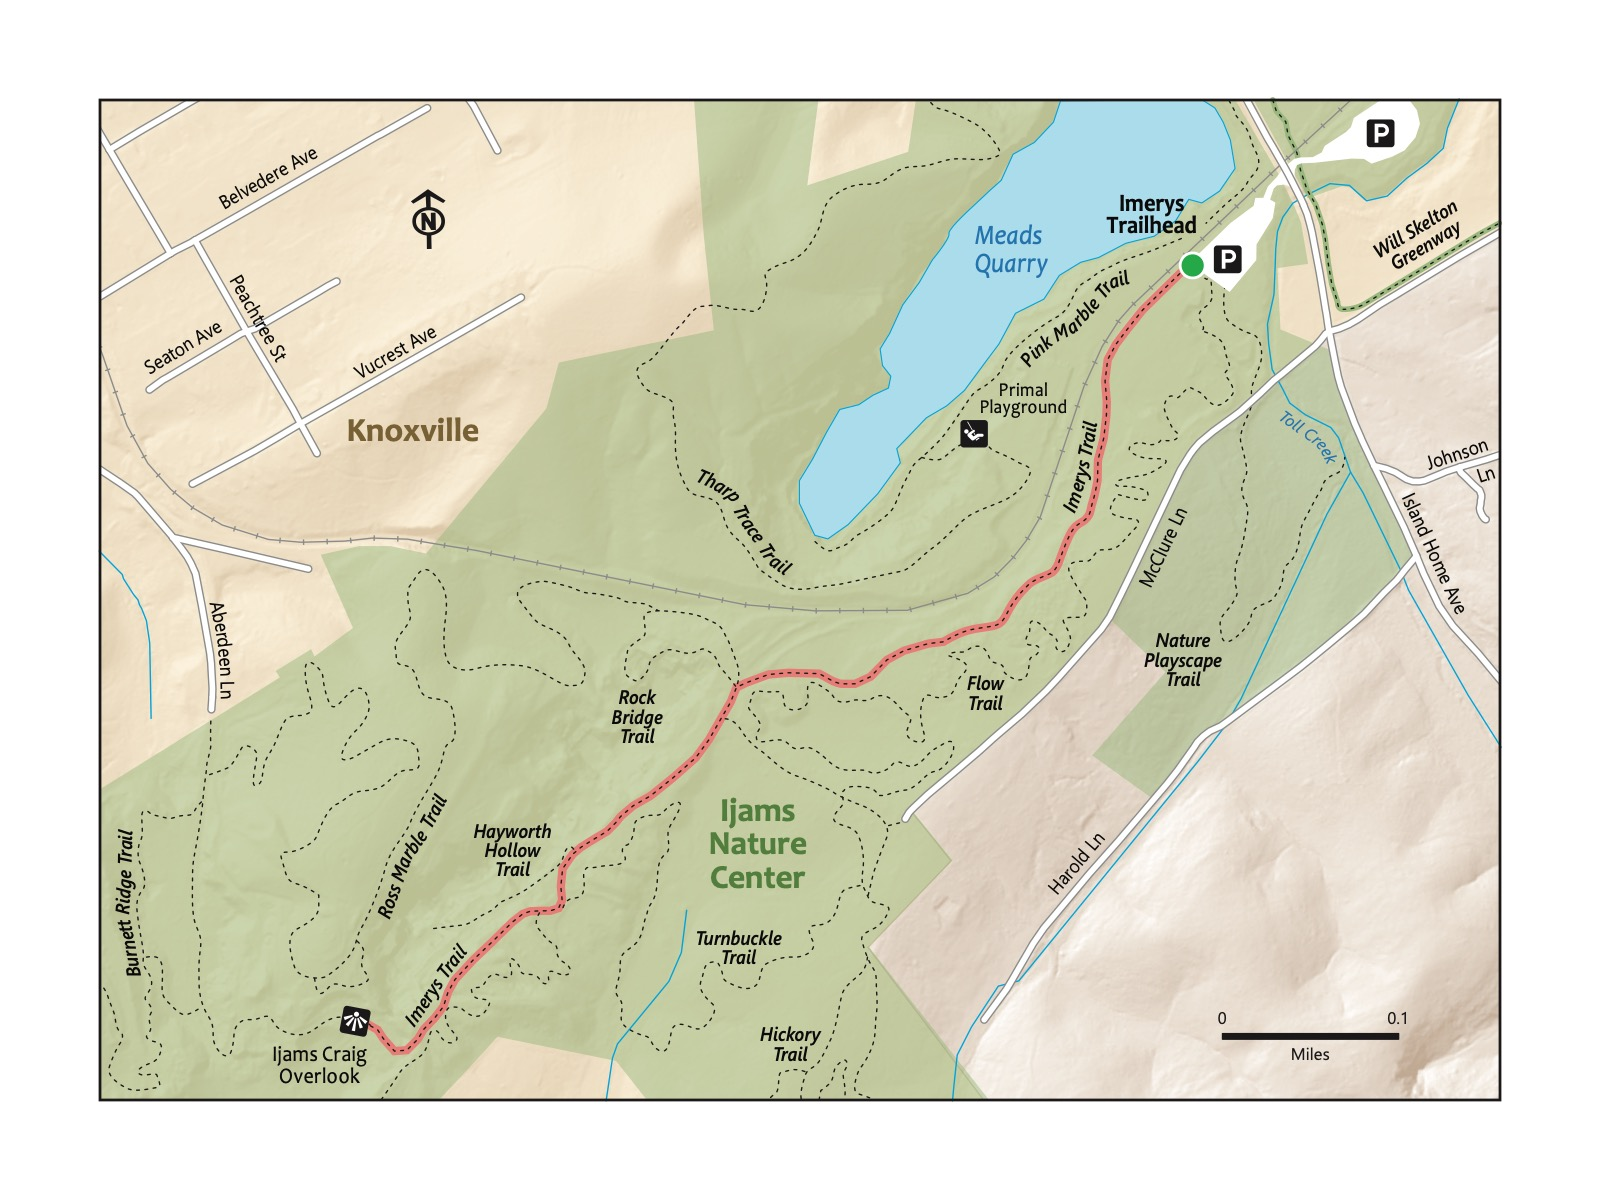
\includegraphics[keepaspectratio]{maps/trail-08-map.jpeg}}

\subsection{Directions to the
Trailhead}\label{directions-to-the-trailhead-7}

Trailhead Address: Meads Quarry, 3526 Island Home Ave, Knoxville, TN
37920

Trailhead GPS Coordinates: 35.95174, -83.86587

\begin{tcolorbox}[enhanced jigsaw, colback=white, colframe=quarto-callout-note-color-frame, breakable, opacityback=0, toprule=.15mm, bottomrule=.15mm, rightrule=.15mm, left=2mm, leftrule=.75mm, arc=.35mm]
\begin{minipage}[t]{5.5mm}
\textcolor{quarto-callout-note-color}{\faInfo}
\end{minipage}%
\begin{minipage}[t]{\textwidth - 5.5mm}

\vspace{-3mm}\textbf{Tennessee Marble}\vspace{3mm}

Mead's Quarry--near the parking area now filled with crystal clear
water--was a quarry for pink-hued Tennessee Marble. This type of marble
was used extensively in prominent buildings in the 1800s and early-mid
1900s, including the National Gallary of Art in Washington, D.C.

\end{minipage}%
\end{tcolorbox}

Park in the parking lot for Meads Quarry using the above address. The
trail begins alongside the disused railroad tracks; look for a sign for
Imery's Trail.

\subsection{Trail Description}\label{trail-description-7}

\begin{longtable}[]{@{}
  >{\raggedright\arraybackslash}p{(\linewidth - 2\tabcolsep) * \real{0.1500}}
  >{\raggedright\arraybackslash}p{(\linewidth - 2\tabcolsep) * \real{0.8500}}@{}}
\toprule\noalign{}
\begin{minipage}[b]{\linewidth}\raggedright
Distance from Start
\end{minipage} & \begin{minipage}[b]{\linewidth}\raggedright
Description
\end{minipage} \\
\midrule\noalign{}
\endhead
\bottomrule\noalign{}
\endlastfoot
0.0 & Start on Imery's trail, heading away from the parking lot. \\
0.15 & Gradually, then more steeply, begin to ascend. \\
0.30 & Trail levels out at an intersection between Imery's Trail, Rock
Bridge Trail, and Gravel Road Trail. \\
0.5 & Rocky and steep. \\
0.75 & Reach the overlook to Ijams Quarry. Rest up, and then turn around
to head back, or continue farther along on Imery's! \\
1.50 & Traihead. \\
\end{longtable}

\subsection{Nearby}\label{nearby-7}

\begin{itemize}
\tightlist
\item
  \textbf{Make sure to stop by the Ijams Visitor Center for a unique
  gift shop and a small collection of local river-based animals!} Check
  out the Ijams River and Tower loop for an introduction to this other
  area of the Ijams Nature Center.
\item
  \textbf{Play at the Ijams Nature Playscape.} This is an amazing part
  of Ijams, worthy of a visit on its own. Tucked away a bit on the side
  of the parking area at Mead's Quarry. It's a favorite for kids, with a
  treehouse, tightrope, stumps for jumping, and, yes, a mud pit!
\item
  \textbf{Check out the Ijams Primal playground.} Also nearby, smaller
  than the Nature Playground, but packed with features for climbing and
  jumping for kids able to climb and explore with little adult
  assistance.
\end{itemize}

\chapter{Trail 9: William Hastie}\label{trail-9-william-hastie}

\subsection{Overview}\label{overview-9}

You'll be surrounded by trees galore at William Hastie! The start
features a beginner's mountain bike loop on a smooth path. Though short,
this hike takes you by many spur trails; consider this a gentle
introduction to a trail system close to but more rustic than Ijams. Good
for all toddling and walking kids and their families.

\begin{figure}[H]

{\centering \pandocbounded{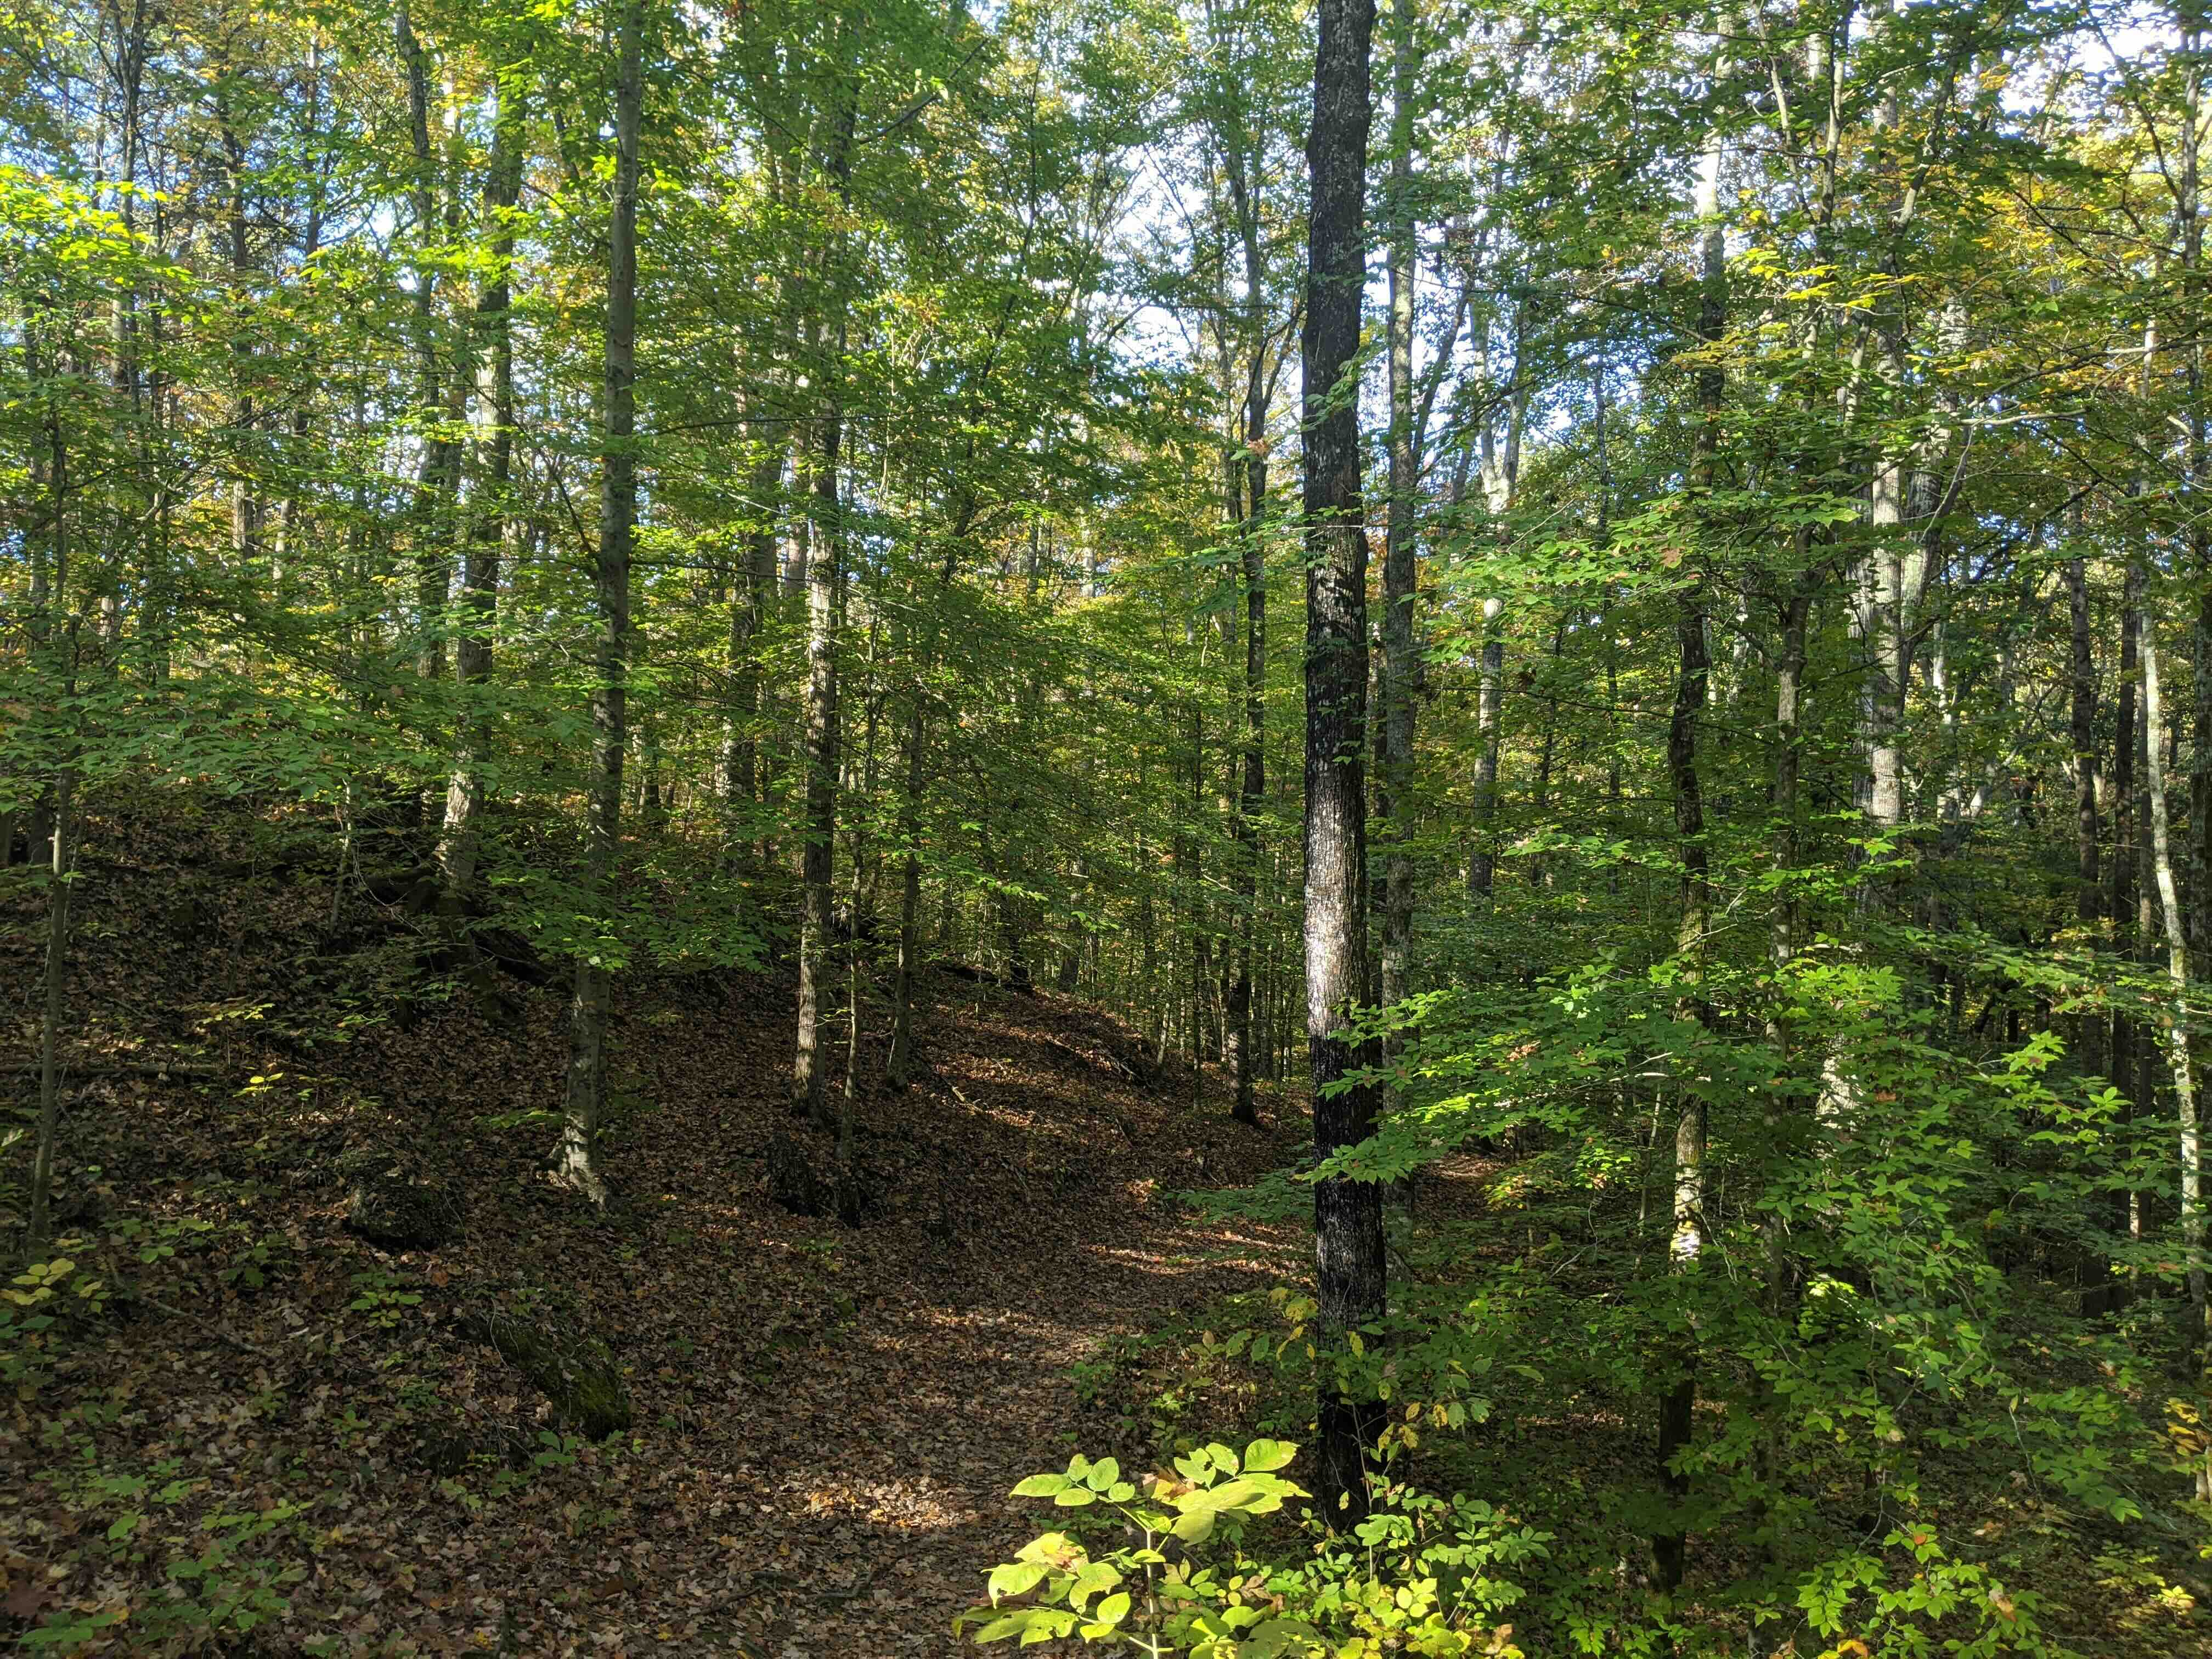
\includegraphics[keepaspectratio]{img/trail-09-figure-01.jpg}}

}

\caption{Photo credit to Katie and Joshua Rosenberg}

\end{figure}%

\subsection{Key Characteristics}\label{key-characteristics-9}

\begin{longtable}[]{@{}
  >{\raggedright\arraybackslash}p{(\linewidth - 2\tabcolsep) * \real{0.5745}}
  >{\raggedright\arraybackslash}p{(\linewidth - 2\tabcolsep) * \real{0.4255}}@{}}
\toprule\noalign{}
\begin{minipage}[b]{\linewidth}\raggedright
\textbf{Characteristic}
\end{minipage} & \begin{minipage}[b]{\linewidth}\raggedright
\textbf{Details}
\end{minipage} \\
\midrule\noalign{}
\endhead
\bottomrule\noalign{}
\endlastfoot
Time Estimate & 0.5 hours - 1 hour \\
Trail Distance (Miles) & 1.3 \\
Elevation Change & Flat \\
Pets & Allowed on leash \\
Parking Pass/Entrance Fee & Not Required \\
Restroom(s) & No \\
Best Ages & Toddlera nd little kids \\
Strollers and Wheelchairs & Partially accessible (graded gravel path) \\
\end{longtable}

\pandocbounded{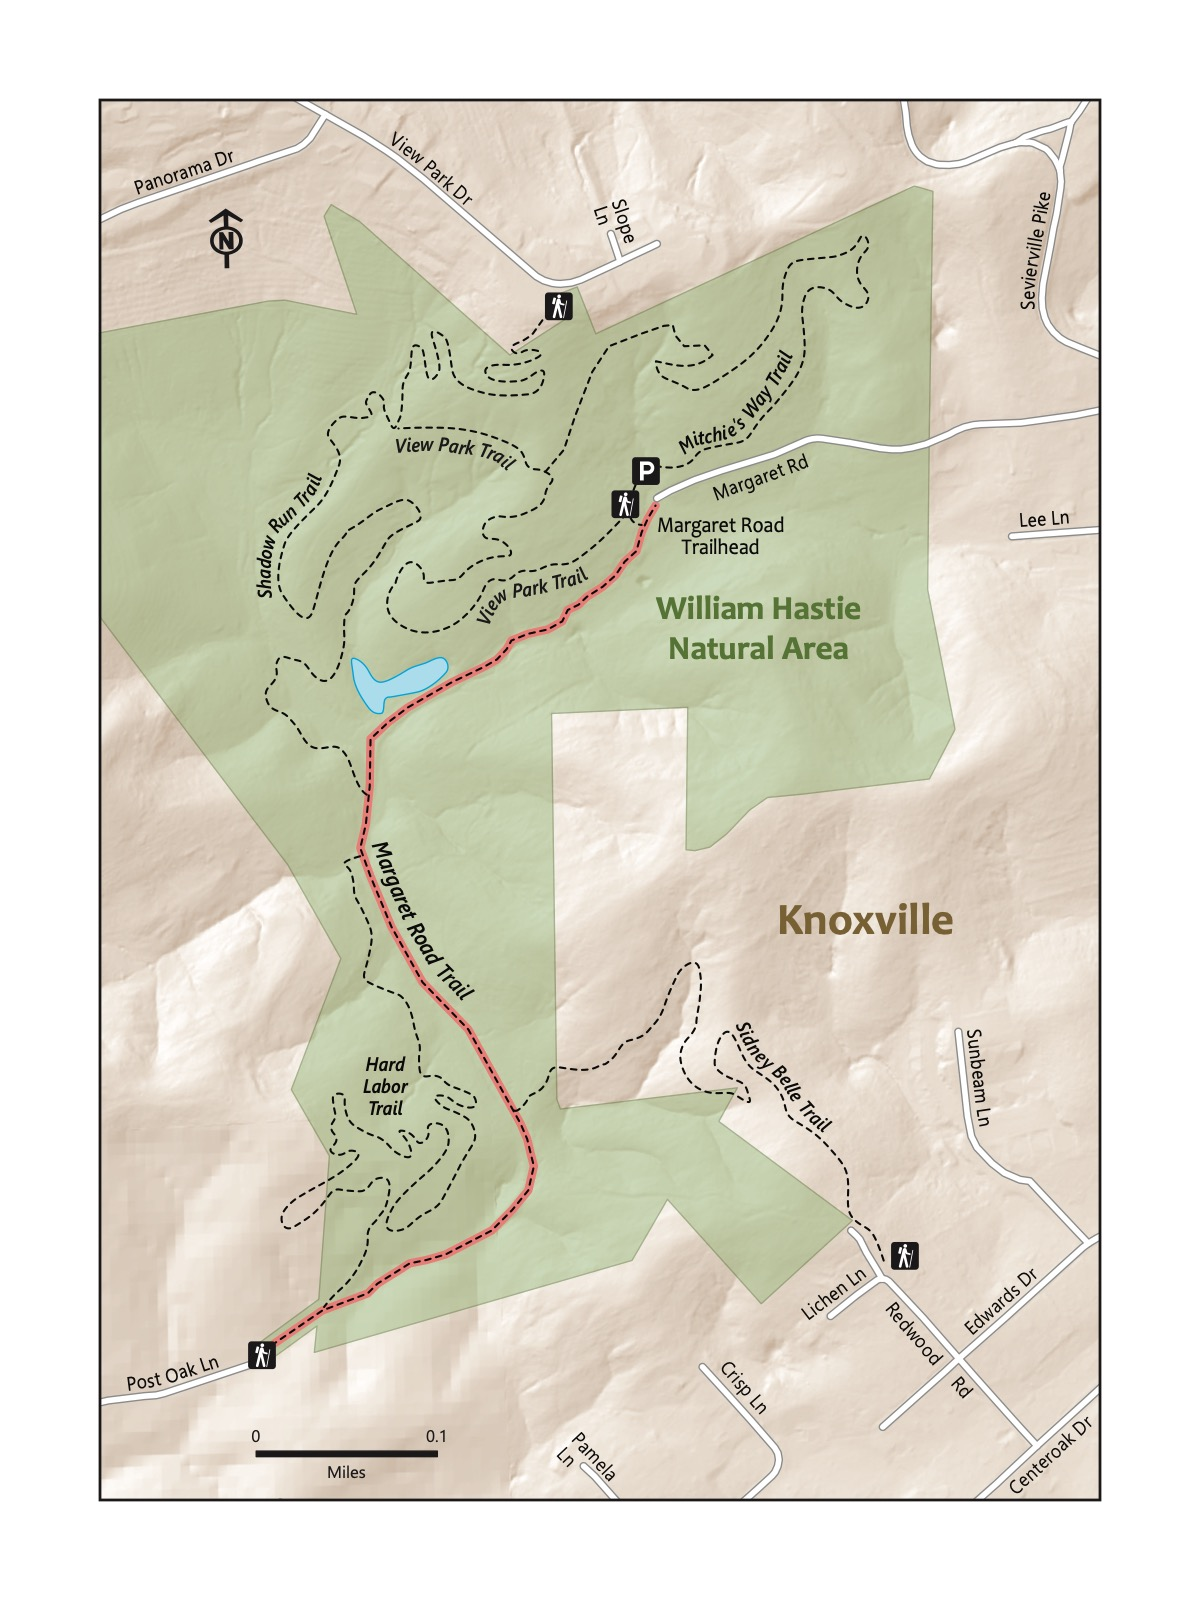
\includegraphics[keepaspectratio]{maps/trail-09-map.jpeg}}

\subsection{Directions to the
Trailhead}\label{directions-to-the-trailhead-8}

Trailhead Address: William Hastie Natural Area, 1302 Margaret Rd,
Knoxville, TN 37920

Trailhead GPS Coordinates: 35.93464, -83.87455

\begin{tcolorbox}[enhanced jigsaw, colback=white, colframe=quarto-callout-note-color-frame, breakable, opacityback=0, toprule=.15mm, bottomrule=.15mm, rightrule=.15mm, left=2mm, leftrule=.75mm, arc=.35mm]
\begin{minipage}[t]{5.5mm}
\textcolor{quarto-callout-note-color}{\faInfo}
\end{minipage}%
\begin{minipage}[t]{\textwidth - 5.5mm}

\vspace{-3mm}\textbf{Eastern Box Turtle}\vspace{3mm}

Think of the Eastern Box Turtle as a tiny explorer. These reptiles
(animals whose body temperature that changes with its surroundings) are
not \emph{necessarily} found only near water. Instead, they move slowly
across the forest floor searching for berries, mushrooms, and insects,
making them easy to observe from a respectful distance. They're smaller
in size than other turtles, with shells around 6'' or fewer in length;
the Snapping Turtle has a far larger shell.

\end{minipage}%
\end{tcolorbox}

The above address will direct you to a large, rarely-busy parking lot
and a nice trailhead with a picnic area. Several trails start from this
trailhead. Look for a sign for the Margaret Road Trail.

\subsection{Trail Description}\label{trail-description-8}

\begin{longtable}[]{@{}
  >{\raggedright\arraybackslash}p{(\linewidth - 2\tabcolsep) * \real{0.2917}}
  >{\raggedright\arraybackslash}p{(\linewidth - 2\tabcolsep) * \real{0.7083}}@{}}
\toprule\noalign{}
\begin{minipage}[b]{\linewidth}\raggedright
Distance from Start
\end{minipage} & \begin{minipage}[b]{\linewidth}\raggedright
Description
\end{minipage} \\
\midrule\noalign{}
\endhead
\bottomrule\noalign{}
\endlastfoot
0.0 & Start on the Margaret Road Trail. \\
0.2 & Small pond on the right. Look for turtles! \\
0.25 & Shadow Run Trail on the right. \\
0.65 & Reach the Post Oak Ln. Trailhead and turn around. \\
1.30 & Traihead. \\
\end{longtable}

\subsection{Nearby}\label{nearby-8}

\begin{itemize}
\tightlist
\item
  \textbf{Bring bike and enjoy the kids' loop.} The ``green'' mountain
  biking trail, Springarn, is a great spot for kids to begin to learn to
  ride on trails. It's only 0.6 miles and is a nice complement to this
  hike.
\item
  \textbf{Explore some of the many other trails while you're there.}
  William Hastie Natural Area features many other trails of varying
  difficulty. Consider taking Mitchie's Way from near the parking
  area---and then looping back to Margaret Road and the start on the
  trail of your choice.
\end{itemize}

\chapter{Trail 10: Sharp's Ridge}\label{trail-10-sharps-ridge}

\subsection{Overview}\label{overview-10}

This hike is just north of downtown, making it a great stop before
grabbing a bite to eat at a nearby restaurant or heading downtown. Wind
up from the trailhead on a smooth path through the pretty forest. When
we think of this trail, we think of little ones toddling or running
ahead around the bends in the trail, just far enough to be out of sight
for a little bit until we catch up! Once you connect to the road,
consider walking up to an overlook with lovely view of the Smokies. Best
for older kids or younger kids who are carried in a carrier or backpack.

\begin{figure}[H]

{\centering \pandocbounded{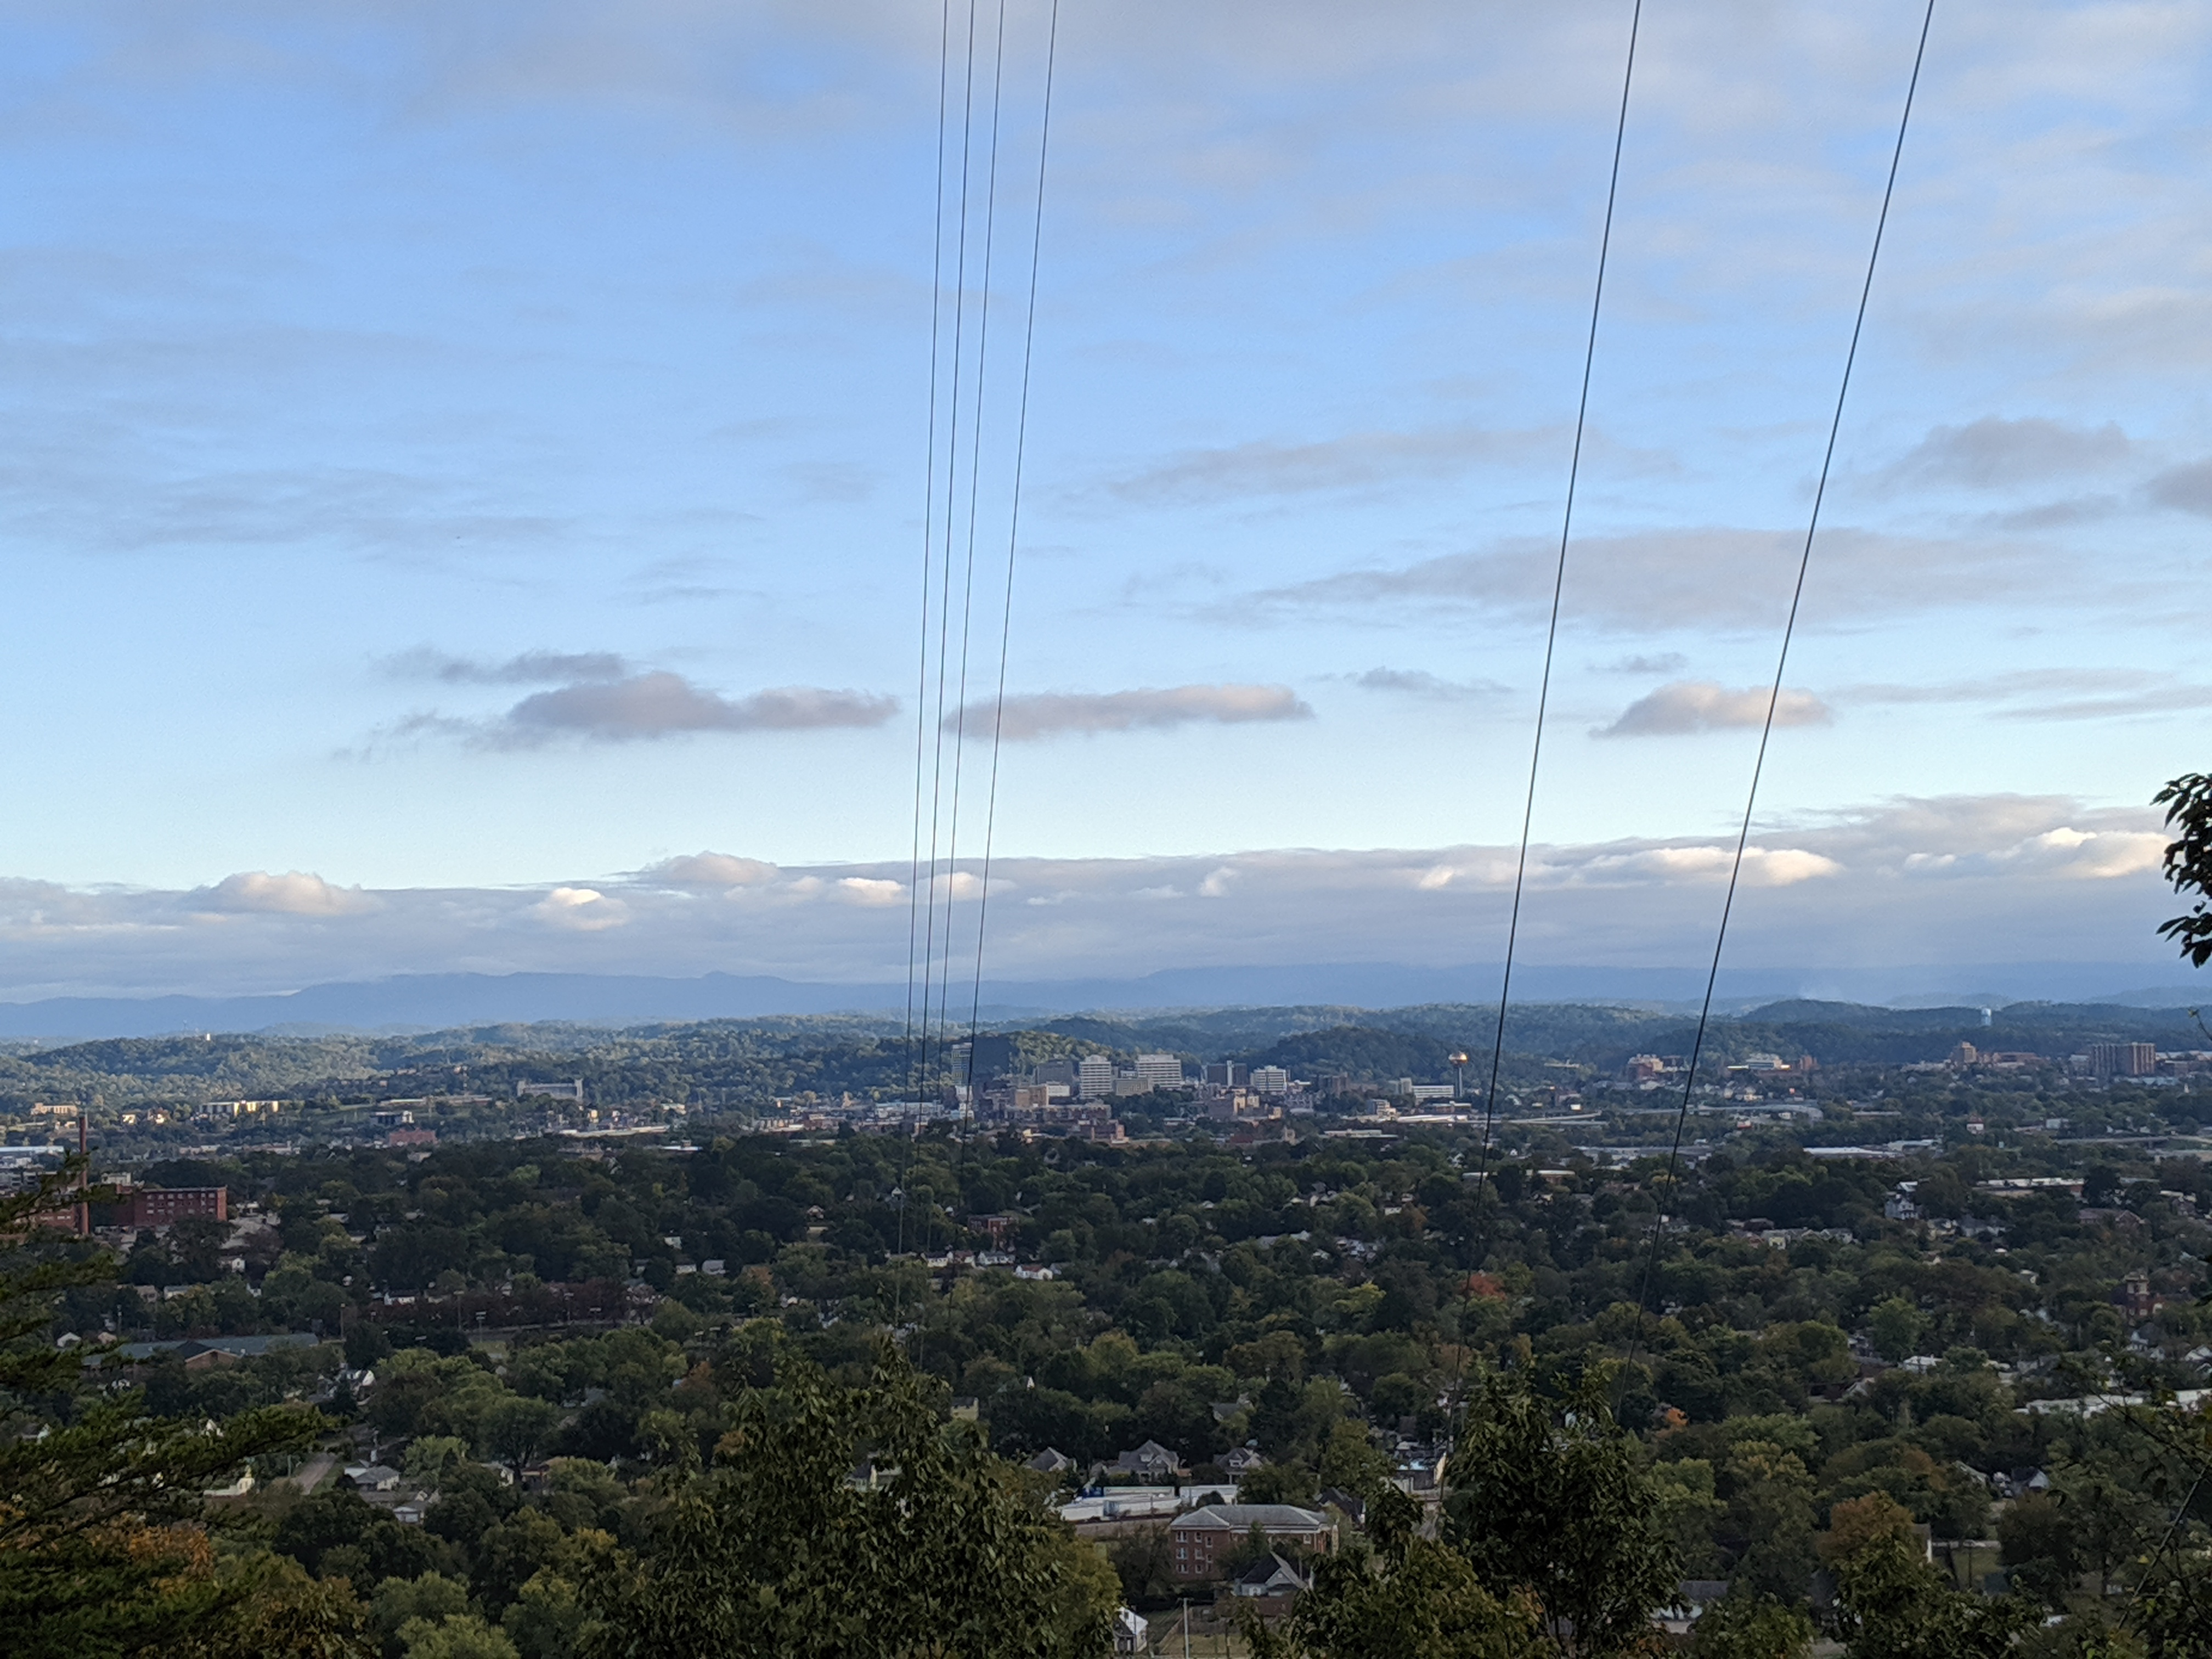
\includegraphics[keepaspectratio]{img/trail-10-figure-01.jpg}}

}

\caption{Photo credit to Katie and Joshua Rosenberg}

\end{figure}%

\subsection{Key Characteristics}\label{key-characteristics-10}

\begin{longtable}[]{@{}ll@{}}
\toprule\noalign{}
\textbf{Characteristic} & \textbf{Details} \\
\midrule\noalign{}
\endhead
\bottomrule\noalign{}
\endlastfoot
Time Estimate & 1.5 hours - 2.5 hours \\
Trail Distance (Miles) & 2.3 \\
Elevation Change & Moderate \\
Pets & Allowed on leash \\
Parking Pass/Entrance Fee & Not Required \\
Restroom(s) & No \\
Best Ages & Little kids \\
Strollers and Wheelchairs & Not accessible \\
\end{longtable}

\pandocbounded{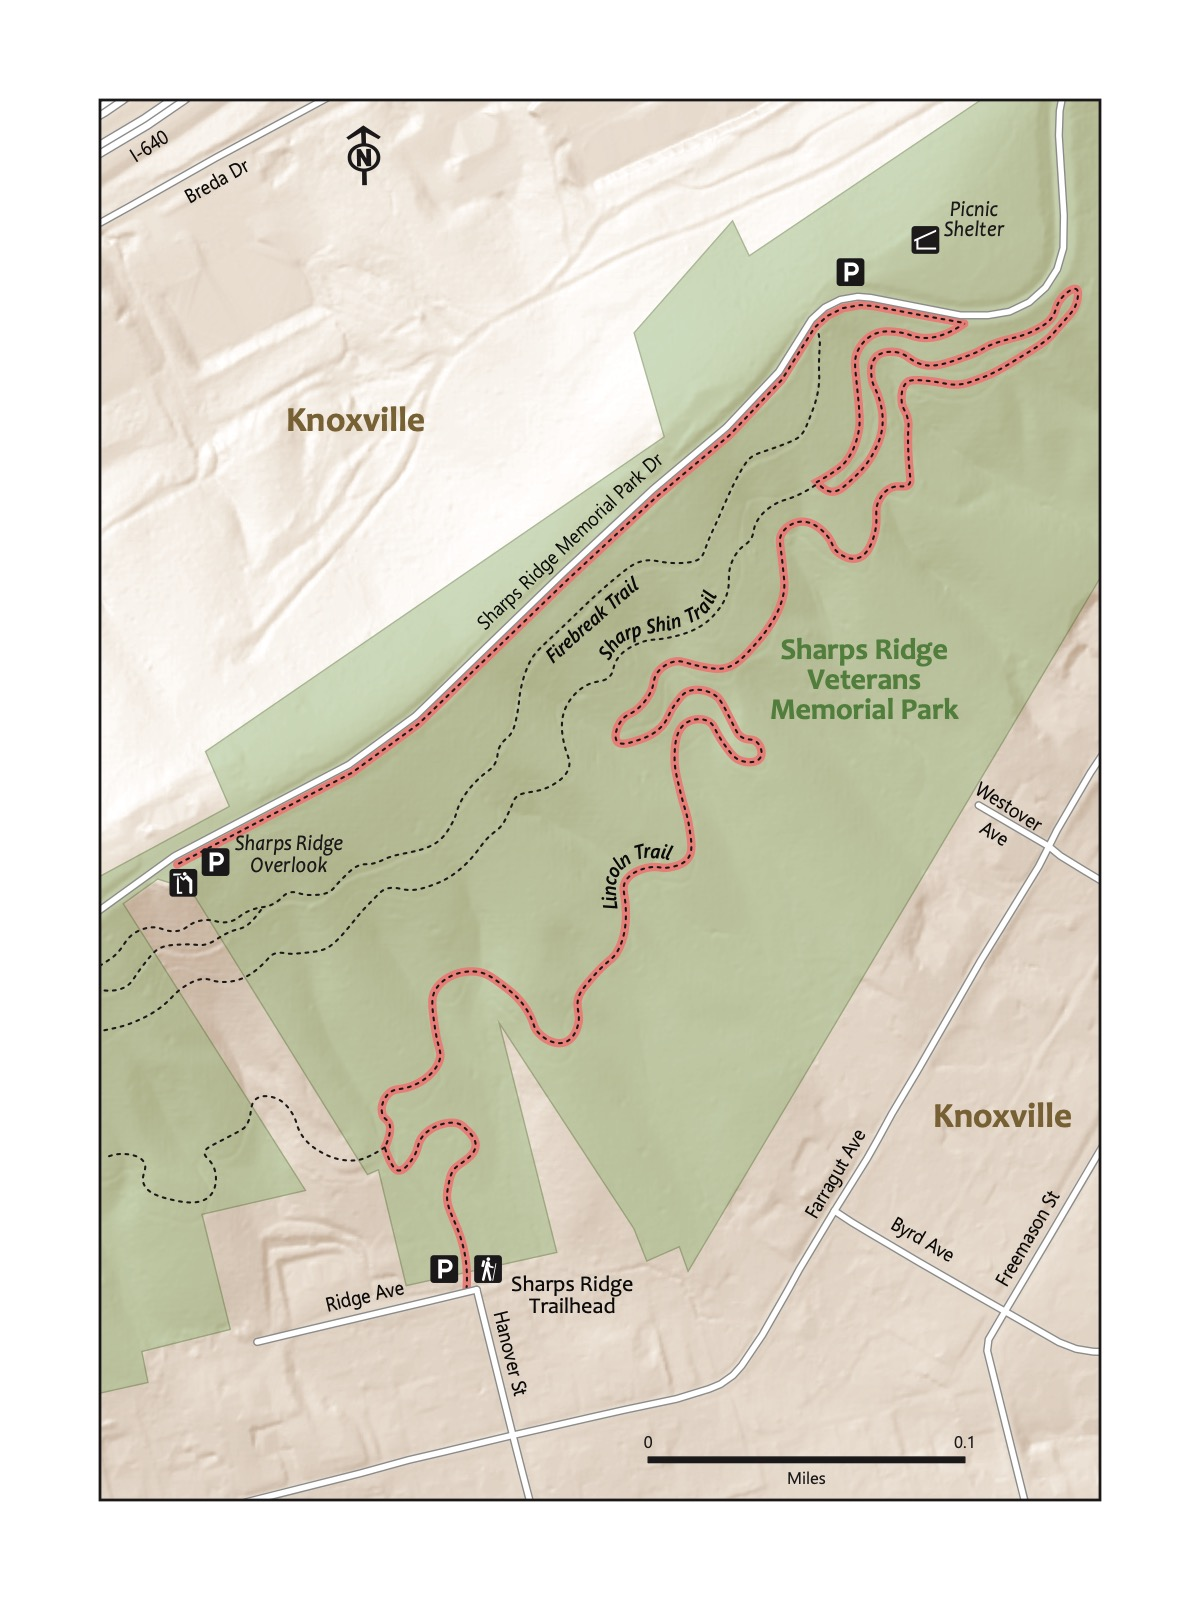
\includegraphics[keepaspectratio]{maps/trail-10-map.jpeg}}

\subsection{Directions to the
Trailhead}\label{directions-to-the-trailhead-9}

Trailhead Address: Sharps Ridge Trailhead, 599-501 Ridge Ave, Knoxville,
TN 37917

Trailhead GPS Coordinates: 36.00344, -83.93787

The trailhead can be just a little tricky to find---partially because
Google Maps has several trailheads with the same name! We once met
friends at different Sharps Ridge Trailheads! Consider putting in the
address (above) to find the trailhead, which is at the end of Hanover
St.~Park in one of the parking spots or the gravel area on the side of
Ridge Ave.

\begin{tcolorbox}[enhanced jigsaw, colback=white, colframe=quarto-callout-note-color-frame, breakable, opacityback=0, toprule=.15mm, bottomrule=.15mm, rightrule=.15mm, left=2mm, leftrule=.75mm, arc=.35mm]
\begin{minipage}[t]{5.5mm}
\textcolor{quarto-callout-note-color}{\faInfo}
\end{minipage}%
\begin{minipage}[t]{\textwidth - 5.5mm}

\vspace{-3mm}\textbf{Lichen}\vspace{3mm}

There are three primary types of lichens: Foliose (leaf-like in
appearance), Crustose (crusty looking), and Fruiticose (coral-like and
bushy). They are abundant in the region and are great bioindicators of
air quality! -Amanda Garner

\end{minipage}%
\end{tcolorbox}

\subsection{Trail Description}\label{trail-description-9}

\begin{longtable}[]{@{}
  >{\raggedright\arraybackslash}p{(\linewidth - 2\tabcolsep) * \real{0.1235}}
  >{\raggedright\arraybackslash}p{(\linewidth - 2\tabcolsep) * \real{0.8765}}@{}}
\toprule\noalign{}
\begin{minipage}[b]{\linewidth}\raggedright
Distance from Start
\end{minipage} & \begin{minipage}[b]{\linewidth}\raggedright
Description
\end{minipage} \\
\midrule\noalign{}
\endhead
\bottomrule\noalign{}
\endlastfoot
0.0 & Start by walking through the Arbor, past the trail map of the
Sharps Ridge area. You're technically on the very short Hanover Access
trail. \\
0.1 & Turn right onto Lincoln Trail. Wind up through the deep woods and
easy curves in the trail. \\
0.8 & Turn right onto Sharp Shin. \\
0.9 & Meet Sharps Ridge Memorial Park Drive. Turn left to walk along the
side of the road toward the overlook, or, alternatively, head back to
the start! \\
1.15 & Overlook. See if you can spy the Sunsphere, Neyland Stadium, and
the Smokies in the distance. Turn around to head back the way you
came. \\
1.4 & Turn right, back onto Sharp Shin. \\
1.5 & Turn left onto Lincoln Trail. \\
2.2 & Turn left onto the Hanover Access Trail. \\
2.3 & Traihead. \\
\end{longtable}

\begin{figure}[H]

{\centering \pandocbounded{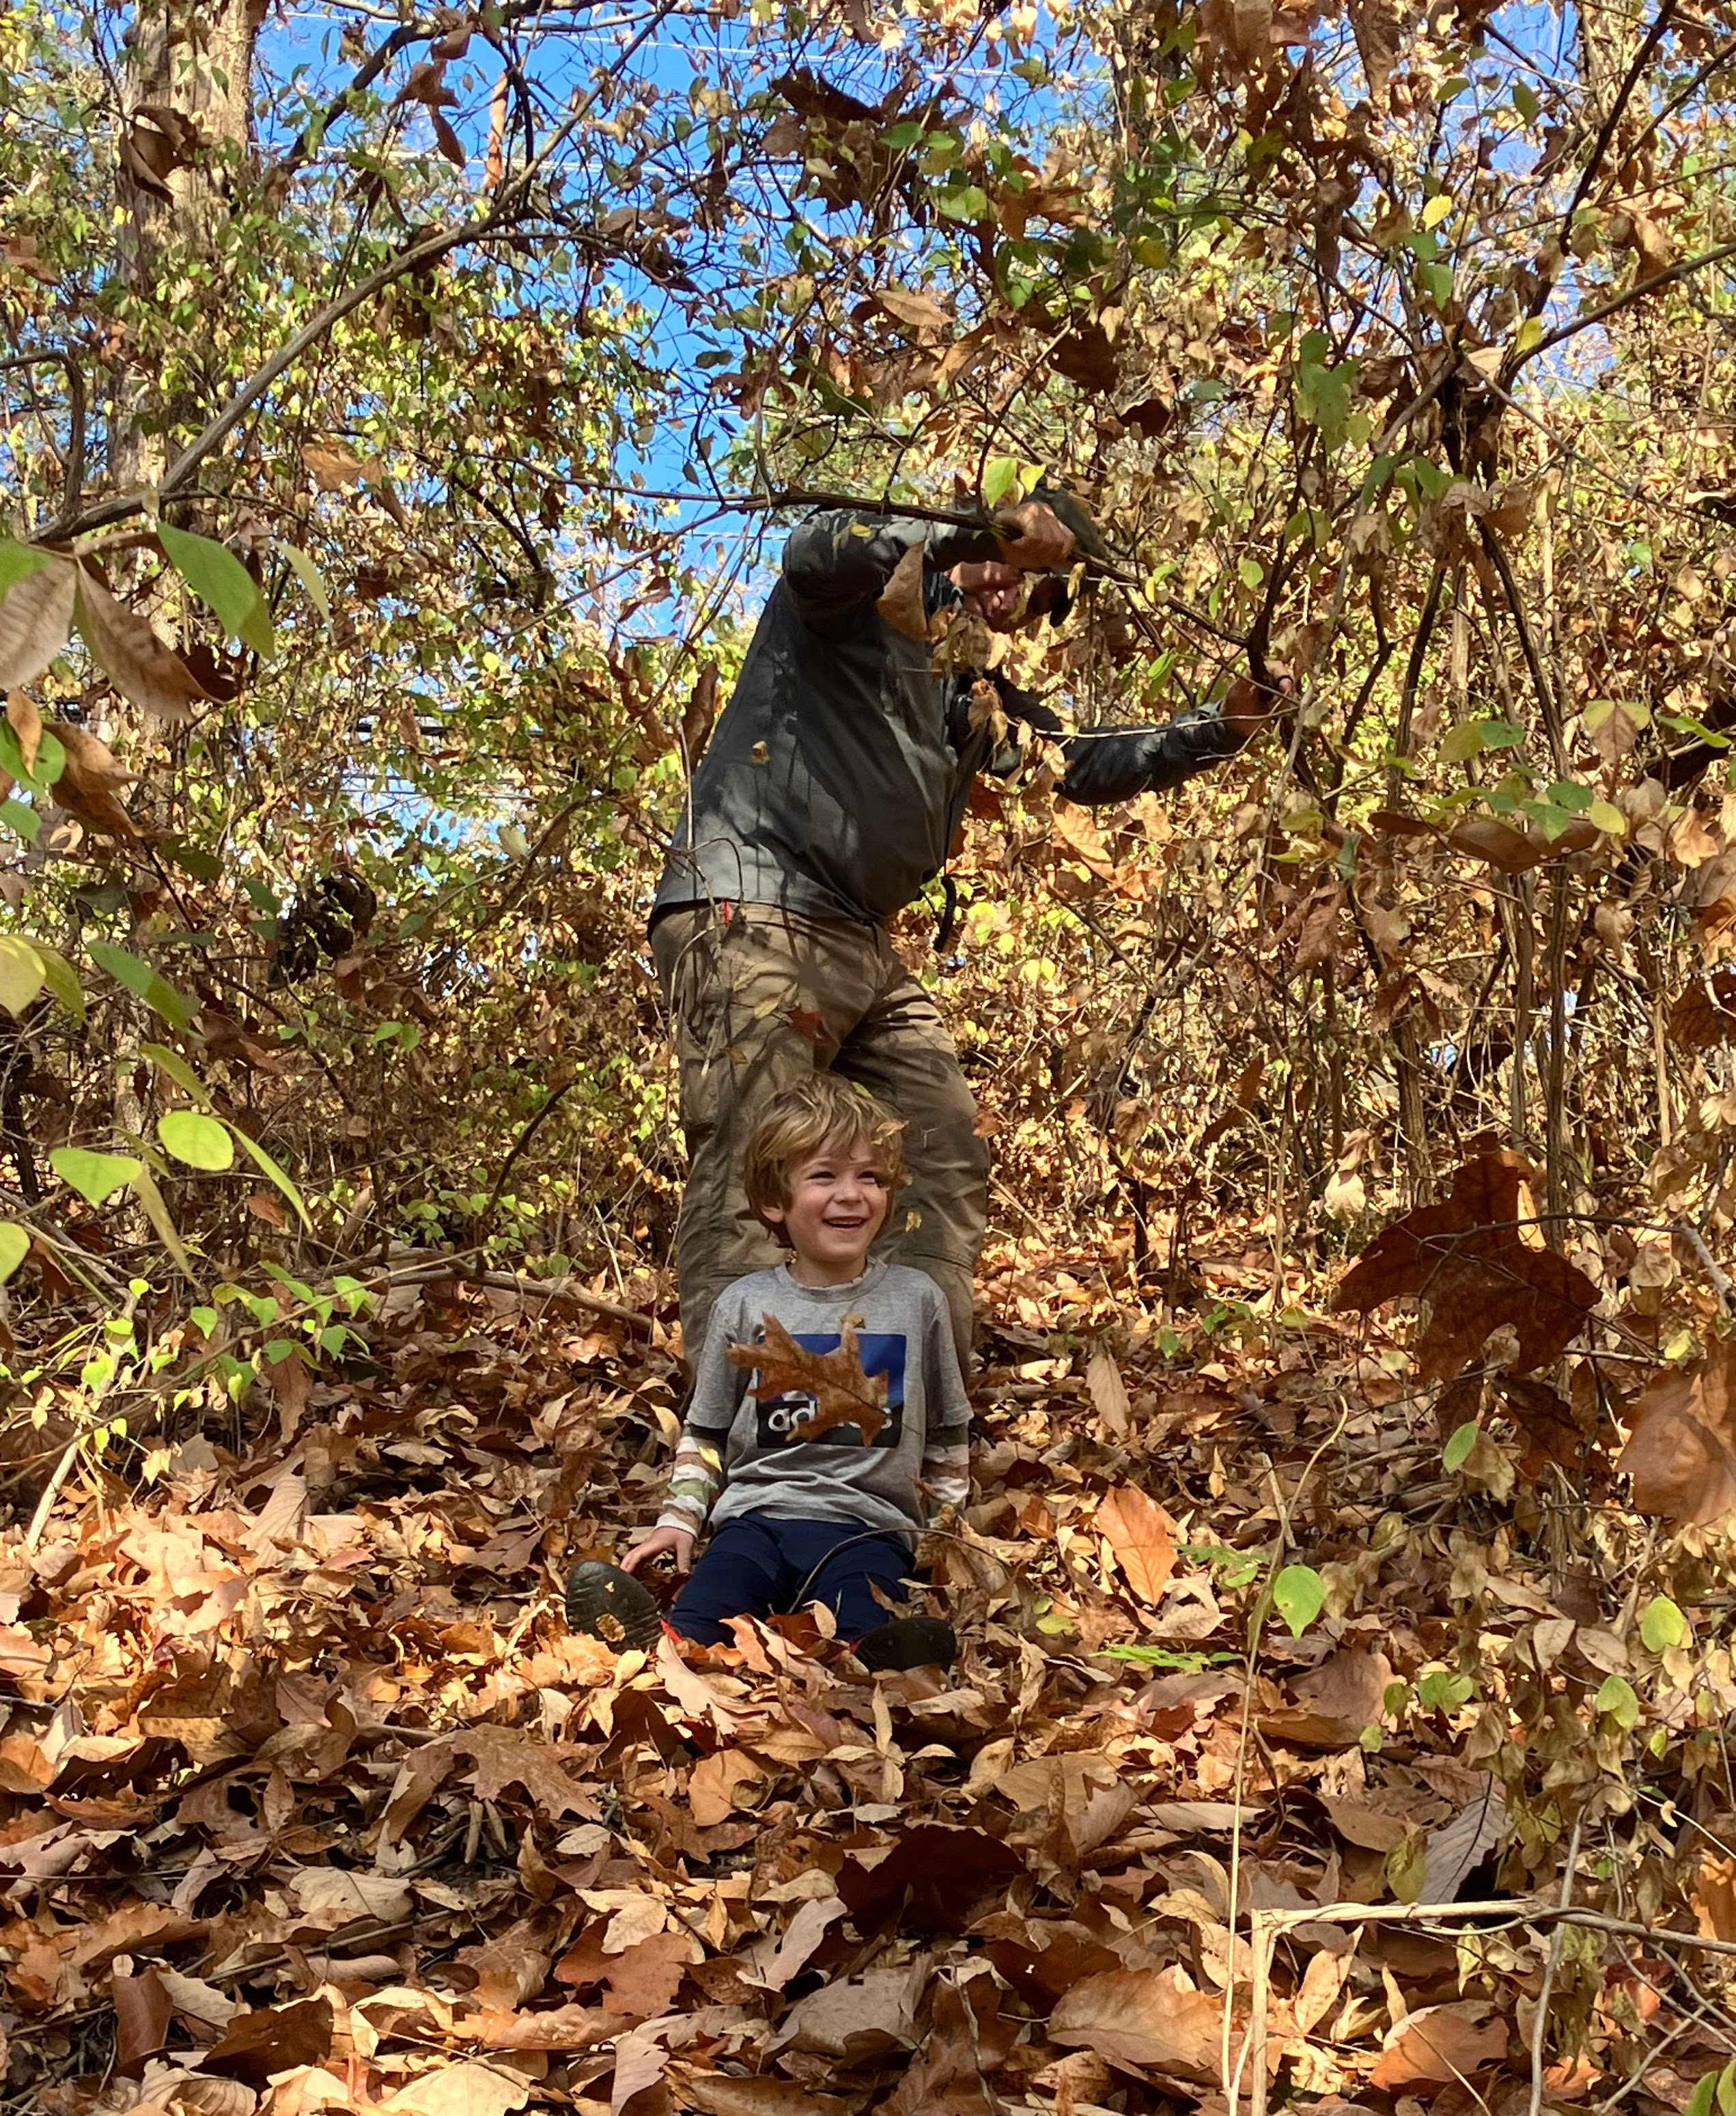
\includegraphics[keepaspectratio]{img/sharps trail.jpg}}

}

\caption{Photo credit to Katie and Joshua Rosenberg}

\end{figure}%

\subsection{Nearby}\label{nearby-9}

\begin{itemize}
\tightlist
\item
  \textbf{Grab a bite to eat at a nearby restaurant.} Favorite nearby
  spots include the fantastic Wild Love Bakehouse (1625 N Central St,
  Knoxville, TN 37917), the quick, inexpensive, tasty Taqueria La
  Herradura (2625 N Broadway, Knoxville, TN 37917), and Hard Knox Pizza
  Central (2300 N Central St, Knoxville, TN 37917).
\item
  \textbf{Hike further or on other trails to keep the adventures
  rolling.} Sharp's Ridge includes many other trails. A favorite starts
  at a different nearby parking area, immediately behind the Cherry
  Creek Apartments (navigate to 3404 Dill St, Knoxville, TN 37917). We
  like the Lincoln Trail, which is also an accessible mountain bike
  trail.
\end{itemize}

\chapter{Trail 11: Norris Dam}\label{trail-11-norris-dam}

\subsection{Overview}\label{overview-11}

If you're looking for a trail that youngest walkers can succeed it, head
north of Knoxville about 30 minutes and check out the Songbird trail at
Norris Dam State Park. Further, it's on a graded gravel path. Like the
Knox-Blount Greenway along the Tennessee River. You may be surprised by
the variety and quantity of wildlife you see along the scenic Clinch
River, which this hike invites you to enjoy as you stroll. This is a
relaxing trail for a family outing that might end with a drive over
Norris Dam or a stop for a bite and a drink at the nearby Clinch River
Brewery. On warmer days, you'll enjoy cooler temps at this riverside
trail due to its location in the valley near water. For toddlers who are
no longer happy in a stroller or backpack carrier, this hike would be a
fun and rewarding challenge!

\begin{figure}[H]

{\centering 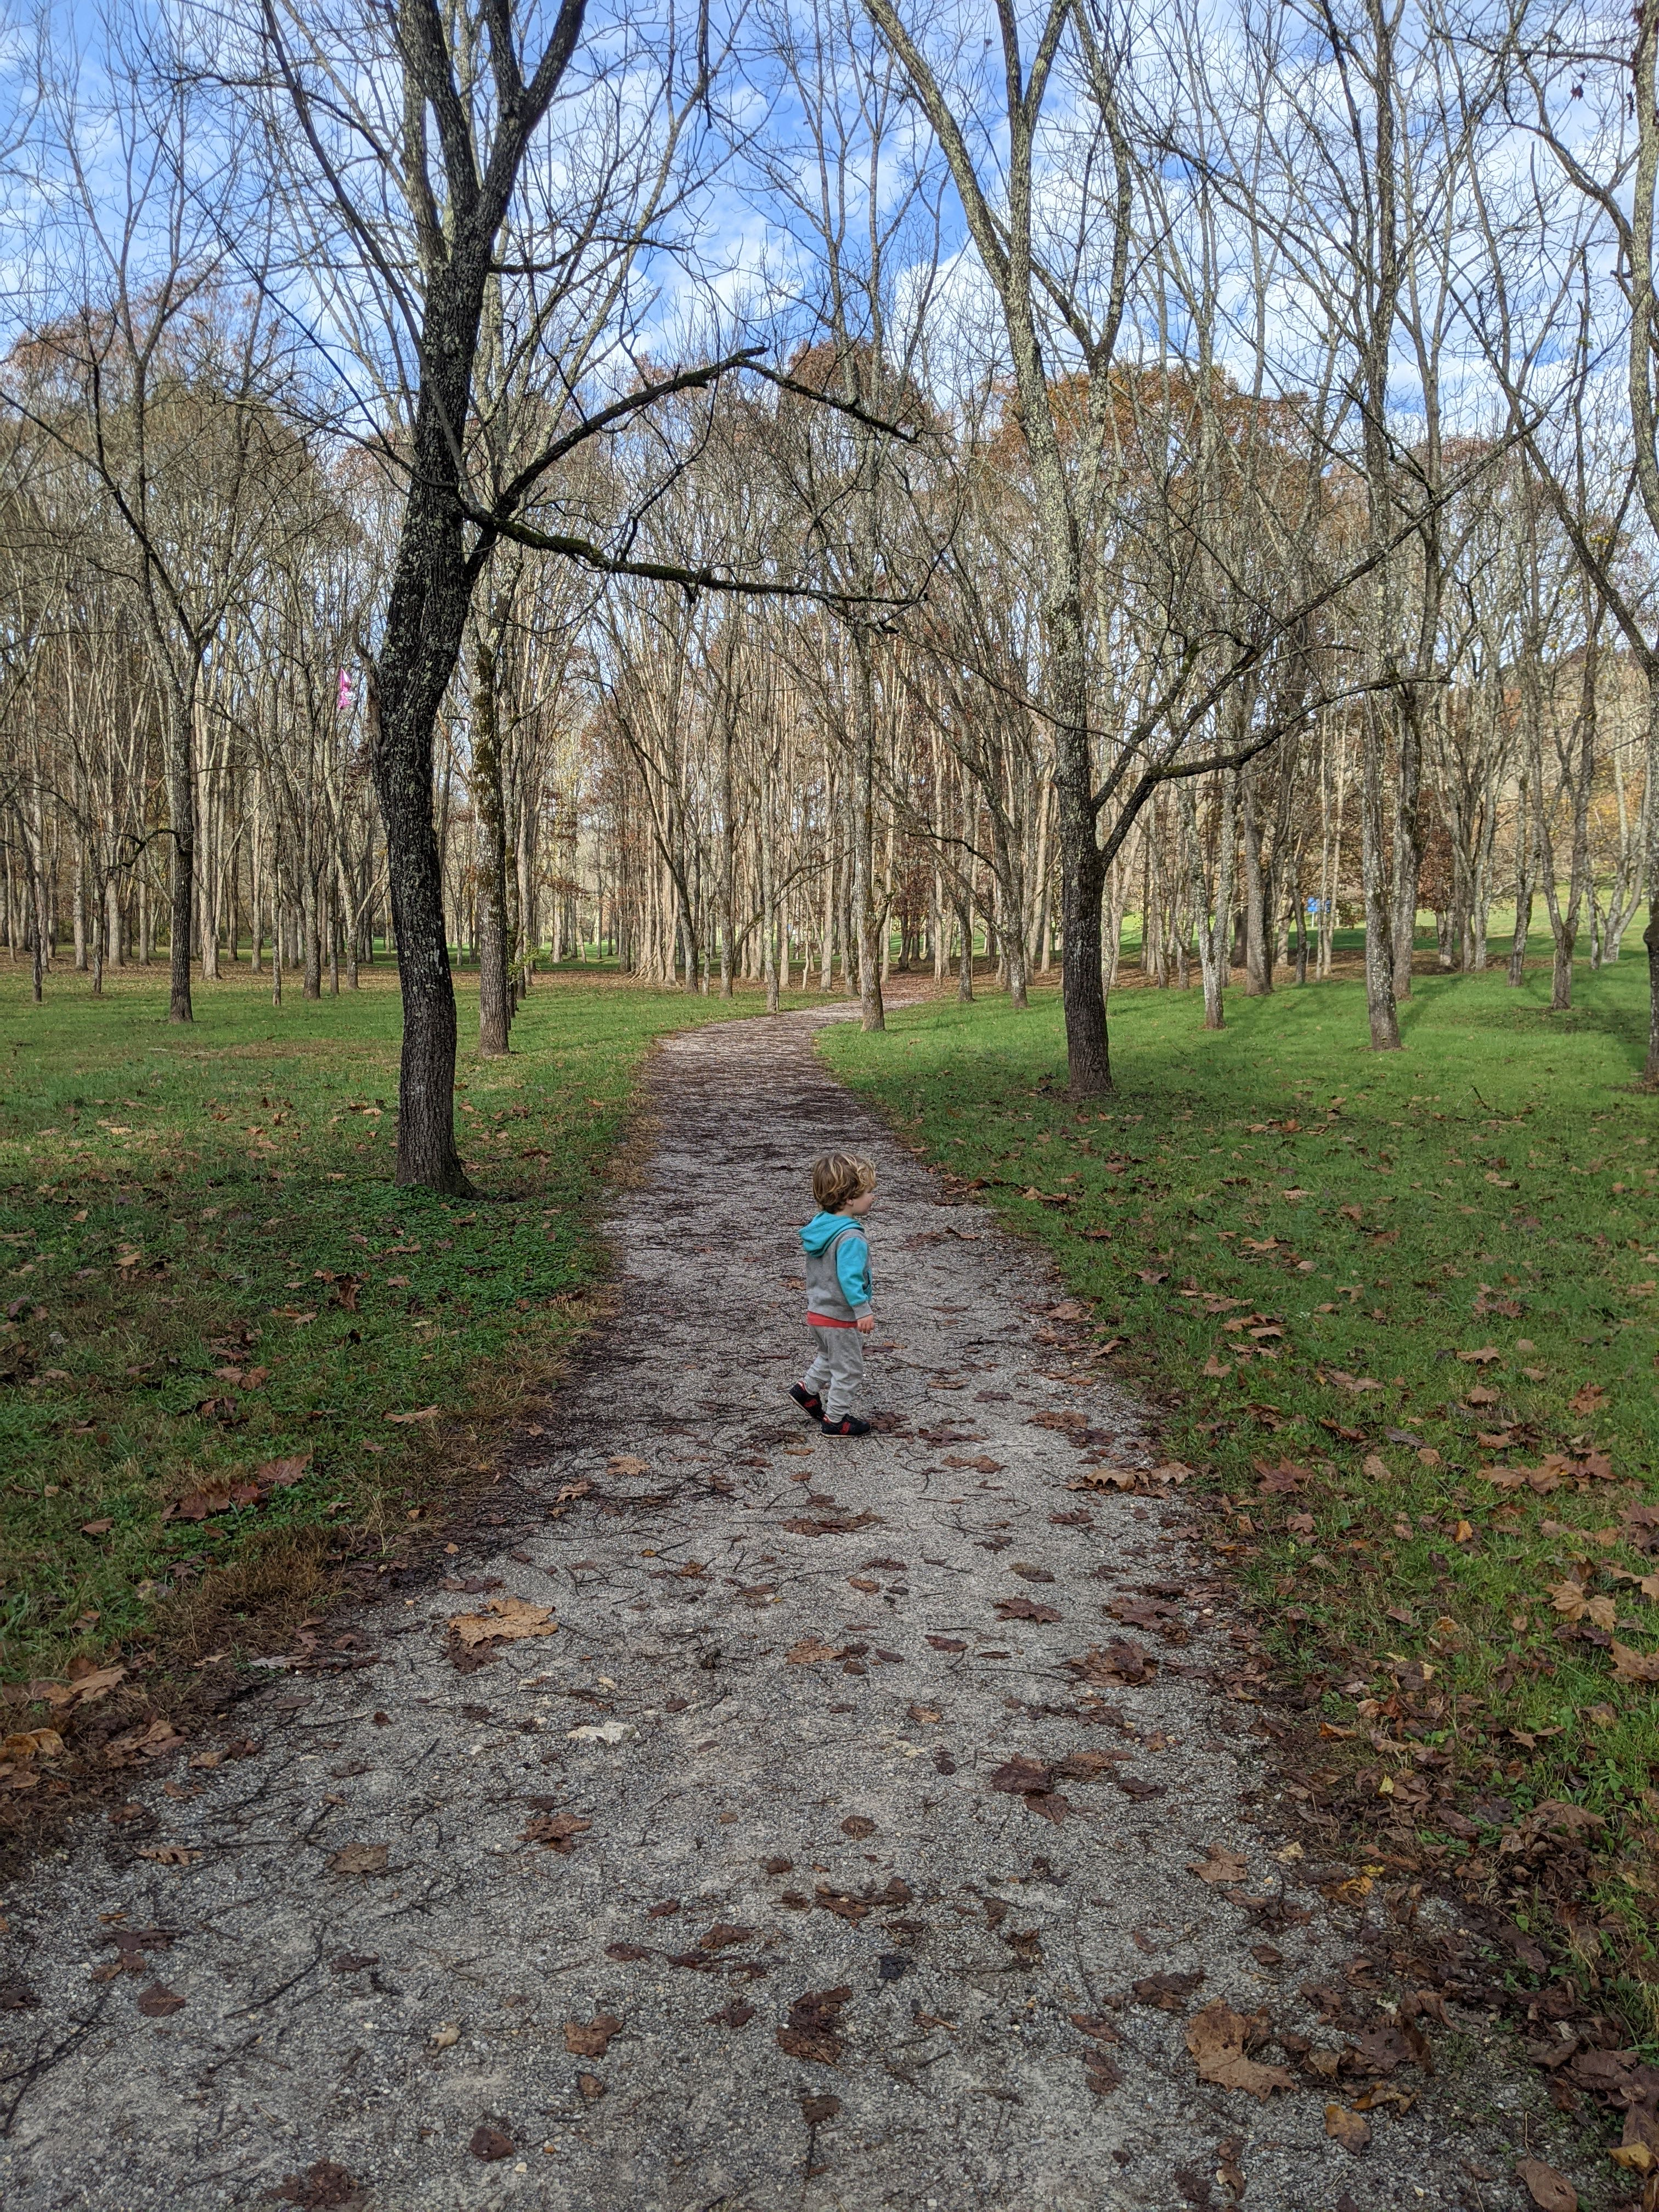
\includegraphics[width=6.25in,height=\textheight,keepaspectratio]{img/trail-11-figure-01.jpg}

}

\caption{Photo credit to Katie and Joshua Rosenberg}

\end{figure}%

\subsection{Key Characteristics}\label{key-characteristics-11}

\begin{longtable}[]{@{}
  >{\raggedright\arraybackslash}p{(\linewidth - 2\tabcolsep) * \real{0.3857}}
  >{\raggedright\arraybackslash}p{(\linewidth - 2\tabcolsep) * \real{0.6143}}@{}}
\toprule\noalign{}
\begin{minipage}[b]{\linewidth}\raggedright
\textbf{Characteristic}
\end{minipage} & \begin{minipage}[b]{\linewidth}\raggedright
\textbf{Details}
\end{minipage} \\
\midrule\noalign{}
\endhead
\bottomrule\noalign{}
\endlastfoot
Time Estimate & 1.5 hours - 2.5 hours \\
Trail Distance (Miles) & 2.3 \\
Elevation Change & Gentle \\
Pets & Allowed on leash \\
Parking Pass/Entrance Fee & Not Required \\
Restroom(s) & No \\
Best Ages & Little kids and Big kids \\
Strollers and Wheelchairs & Partially accessible (graded gravel path) \\
\end{longtable}

\pandocbounded{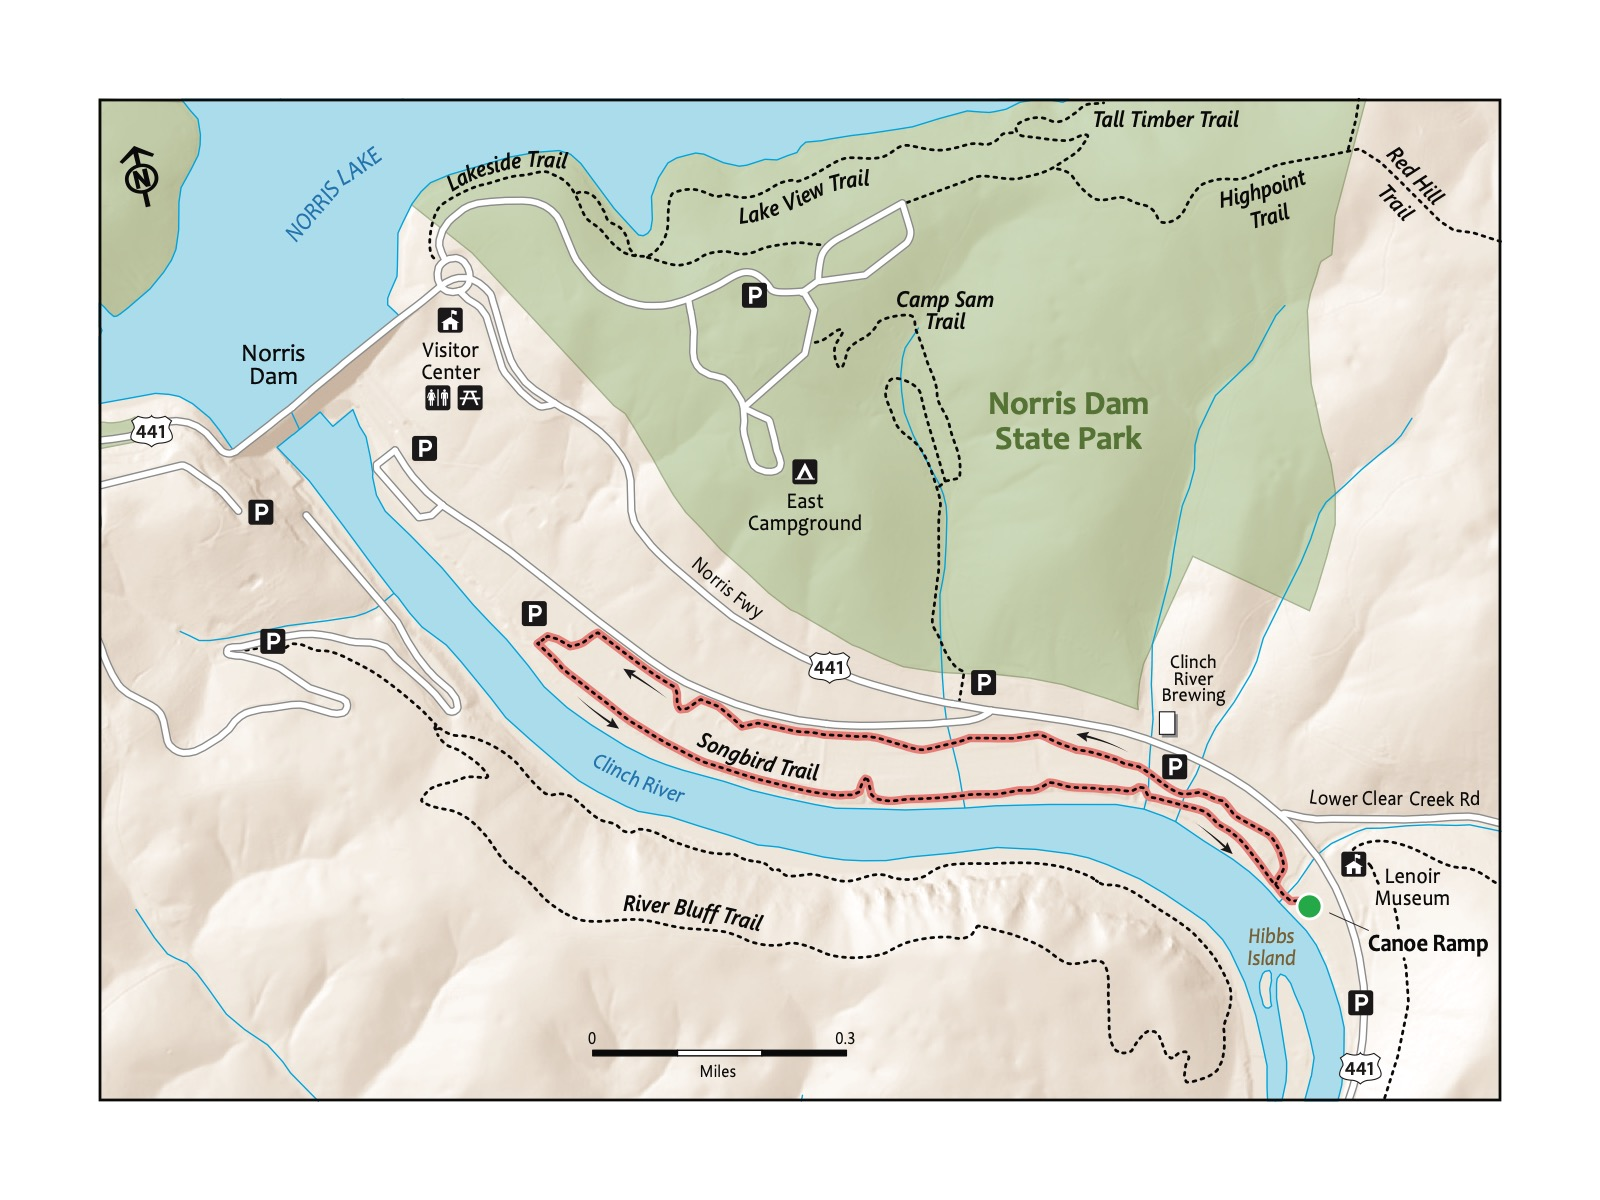
\includegraphics[keepaspectratio]{maps/trail-11-map.jpeg}}

\subsection{Directions to the
Trailhead}\label{directions-to-the-trailhead-10}

Trailhead Address: Canoe Ramp by the Songbird Loop, 6W6G+R7 Rocky Top,
Tennessee

Trailhead GPS Coordinates: 36.21210, -84.07397

\begin{tcolorbox}[enhanced jigsaw, colback=white, colframe=quarto-callout-note-color-frame, breakable, opacityback=0, toprule=.15mm, bottomrule=.15mm, rightrule=.15mm, left=2mm, leftrule=.75mm, arc=.35mm]
\begin{minipage}[t]{5.5mm}
\textcolor{quarto-callout-note-color}{\faInfo}
\end{minipage}%
\begin{minipage}[t]{\textwidth - 5.5mm}

\vspace{-3mm}\textbf{Norris Dam}\vspace{3mm}

This was the first dam built by the Tennessee Valley Authority,
stretching more than 1,800 feet wide and soaring 265 feet high. Behind
it lies Norris Lake, a favorite for paddling and boating, while the
Clinch River flows just below.

\end{minipage}%
\end{tcolorbox}

There are several possible trailheads. We chose to start this hike from
a put in spot for kayaks and canoes. In Google Maps, you can search the
above address. Please note it uses a ``Plus code'' instead of a street
address, as the canoe ramp does not have an address. This is immediately
off Norris Fwy. (Highway 441).

\subsection{Trail Description}\label{trail-description-10}

\begin{longtable}[]{@{}
  >{\raggedright\arraybackslash}p{(\linewidth - 2\tabcolsep) * \real{0.2059}}
  >{\raggedright\arraybackslash}p{(\linewidth - 2\tabcolsep) * \real{0.7941}}@{}}
\toprule\noalign{}
\begin{minipage}[b]{\linewidth}\raggedright
Distance from Start
\end{minipage} & \begin{minipage}[b]{\linewidth}\raggedright
Description
\end{minipage} \\
\midrule\noalign{}
\endhead
\bottomrule\noalign{}
\endlastfoot
0.0 & Cross a short bridge over Clear Creek. \\
0.05 & Turn right (though, it is a loop and you may choose to go the
other other way). \\
0.3 & Cross a short bridge. \\
1.0 & Turn left, toward the river, remaining on the same trail. \\
1.05 & Follow the trail back along the river. \\
2.3 & Trailhead. \\
\end{longtable}

\subsection{Nearby}\label{nearby-10}

\begin{itemize}
\tightlist
\item
  \textbf{Grab a bite and a drink Clinch River Brewery.} Clinch River
  Brewing (2045 Norris Fwy, Norris, TN 37828) is not within the
  boundaries of the Norris Dam State Park---but it's very close to the
  trailhead and is a fun place to stop for lunch or dinner before or
  after a hike.
\item
  \textbf{Check out the Norris Dam, which has been in operation since
  the mid-1930s.} Stop at the TVA Norris Dam Visitor Center on the same
  side of the Clinch River as this hike---or drive across and back over
  the dam for an impressive, even otherworldly experience!
\end{itemize}

\begin{figure}[H]

{\centering \pandocbounded{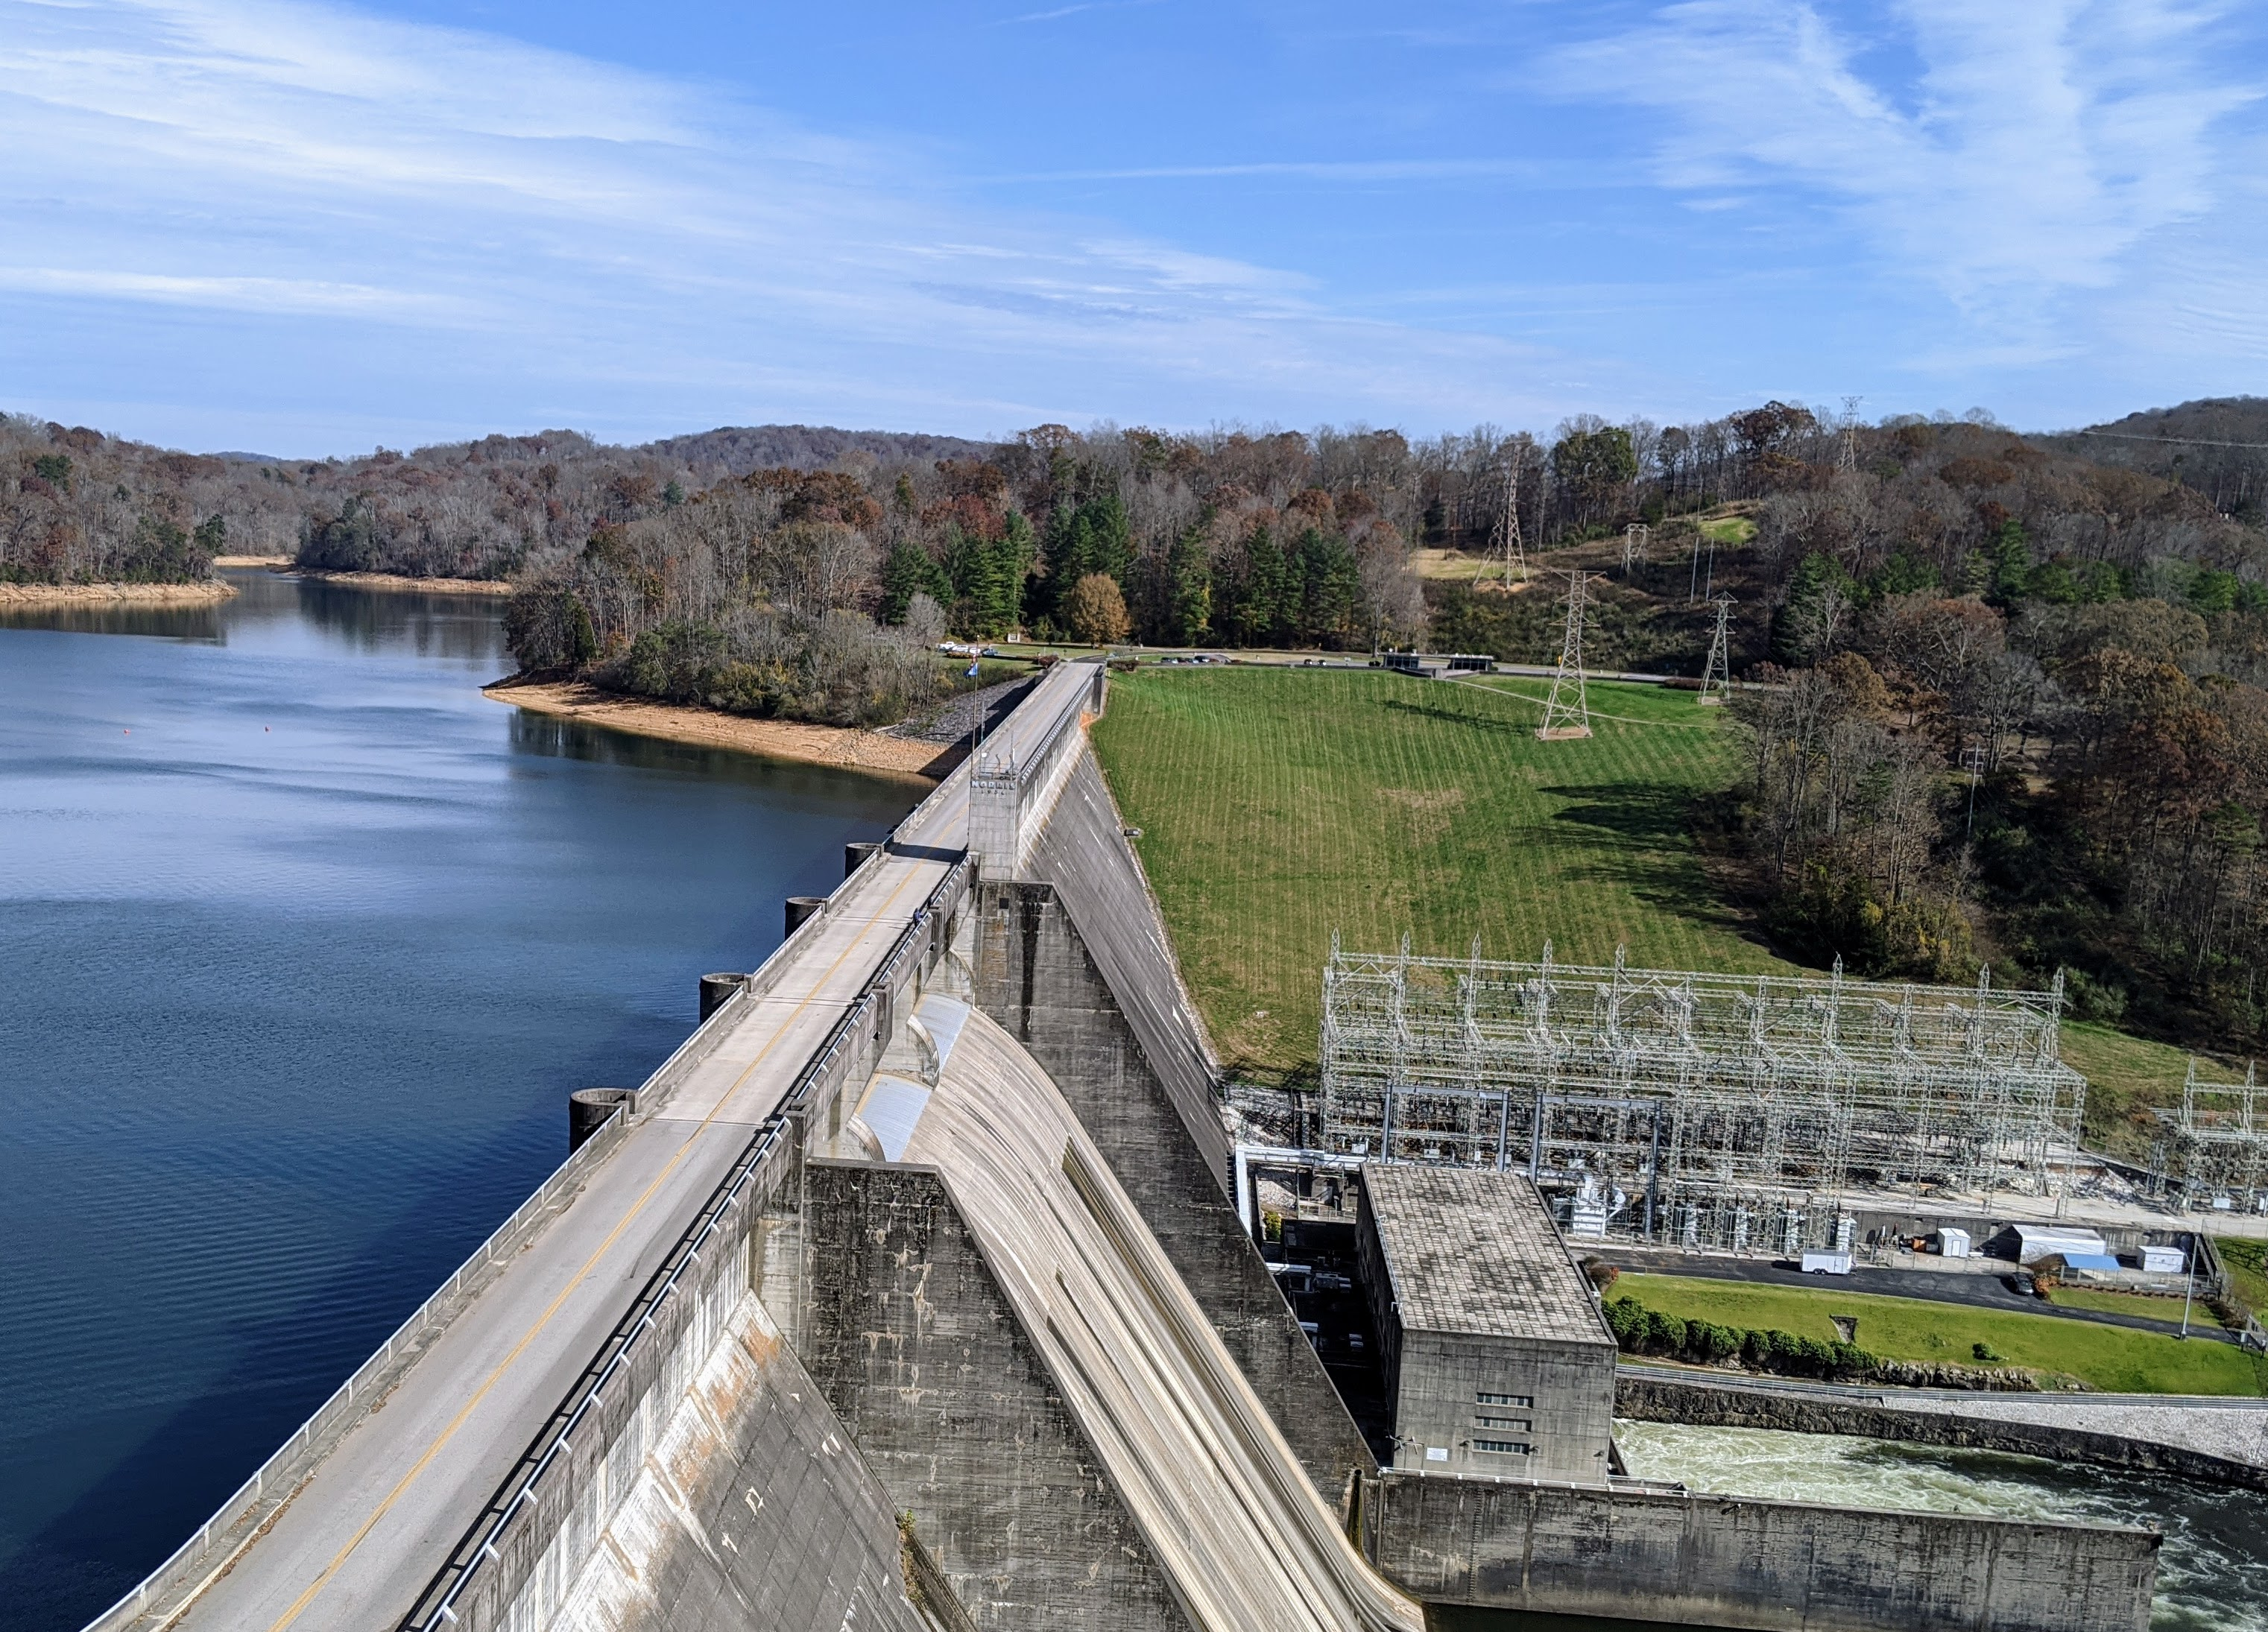
\includegraphics[keepaspectratio]{img/norris dam.jpg}}

}

\caption{Photo credit to Katie and Joshua Rosenberg}

\end{figure}%

\chapter{Trail 12: House Mountain}\label{trail-12-house-mountain}

\subsection{Overview}\label{overview-12}

This hike is not for the faint of heart! Perhaps this comes as a
surprise given its proximity to Knoxville, but this hike features
significant elevation change, rocky and uneven terrain, and even
sections where it is unclear where precisely the trail goes. If you have
littles that need to be carried, we recommend waiting to tackle this
hike (Katie carried our oldest in a baby carrier up this hike when he
was a baby and will honestly tell you she doesn't have fond memories of
this hike). This one always challenges us, but the flip side is that
House Mountain offers a hike that is very rewarding and challenging hike
closer to home than you would expect. The trail climbs up House Mountain
from the west, reaching the West Overlook before heading down to
complete the loop.

\begin{figure}[H]

{\centering \pandocbounded{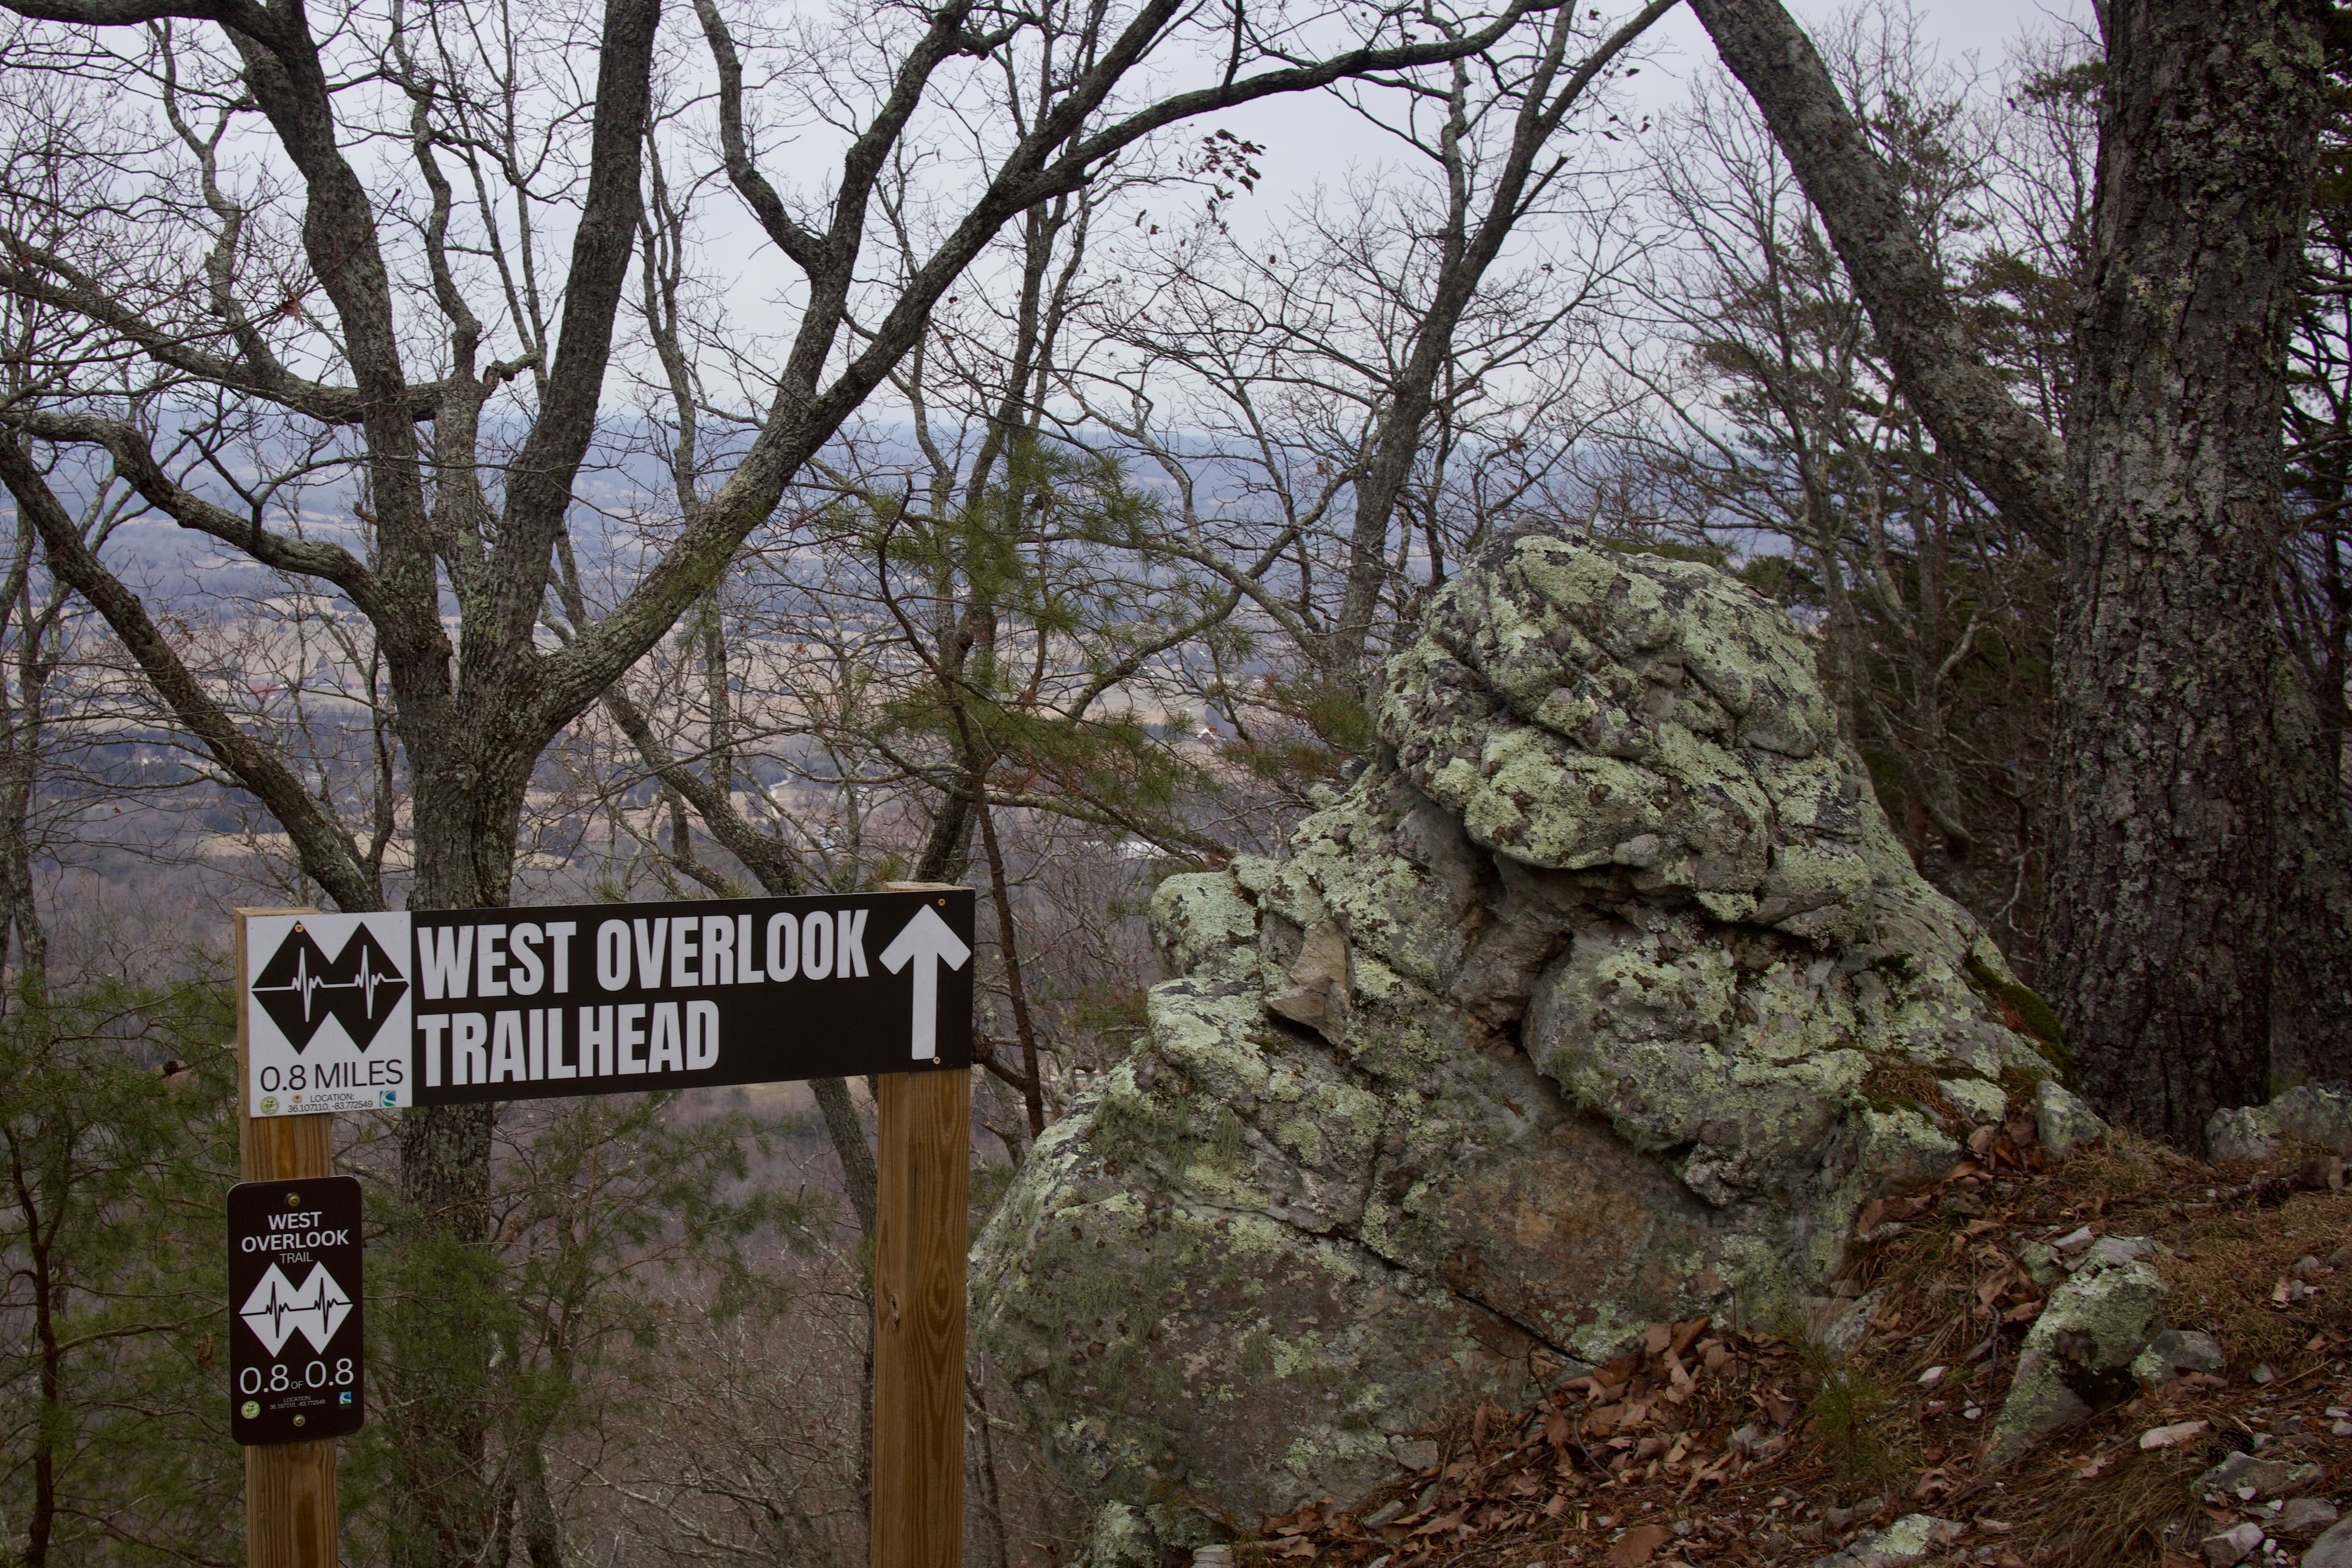
\includegraphics[keepaspectratio]{img/trail-12-figure-01.jpg}}

}

\caption{Photo credit to Katie and Joshua Rosenberg}

\end{figure}%

\subsection{Key Characteristics}\label{key-characteristics-12}

\begin{longtable}[]{@{}ll@{}}
\toprule\noalign{}
\textbf{Characteristic} & \textbf{Details} \\
\midrule\noalign{}
\endhead
\bottomrule\noalign{}
\endlastfoot
Time Estimate & 2.5 hours - 4.5 hours \\
Trail Distance (Miles) & 2.5 \\
Elevation Change & Steep \\
Pets & Allowed on leash \\
Parking Pass/Entrance Fee & Not Required \\
Restroom(s) & No \\
Best Ages & Pre-teens and older \\
Strollers and Wheelchairs & Not accessible \\
\end{longtable}

\pandocbounded{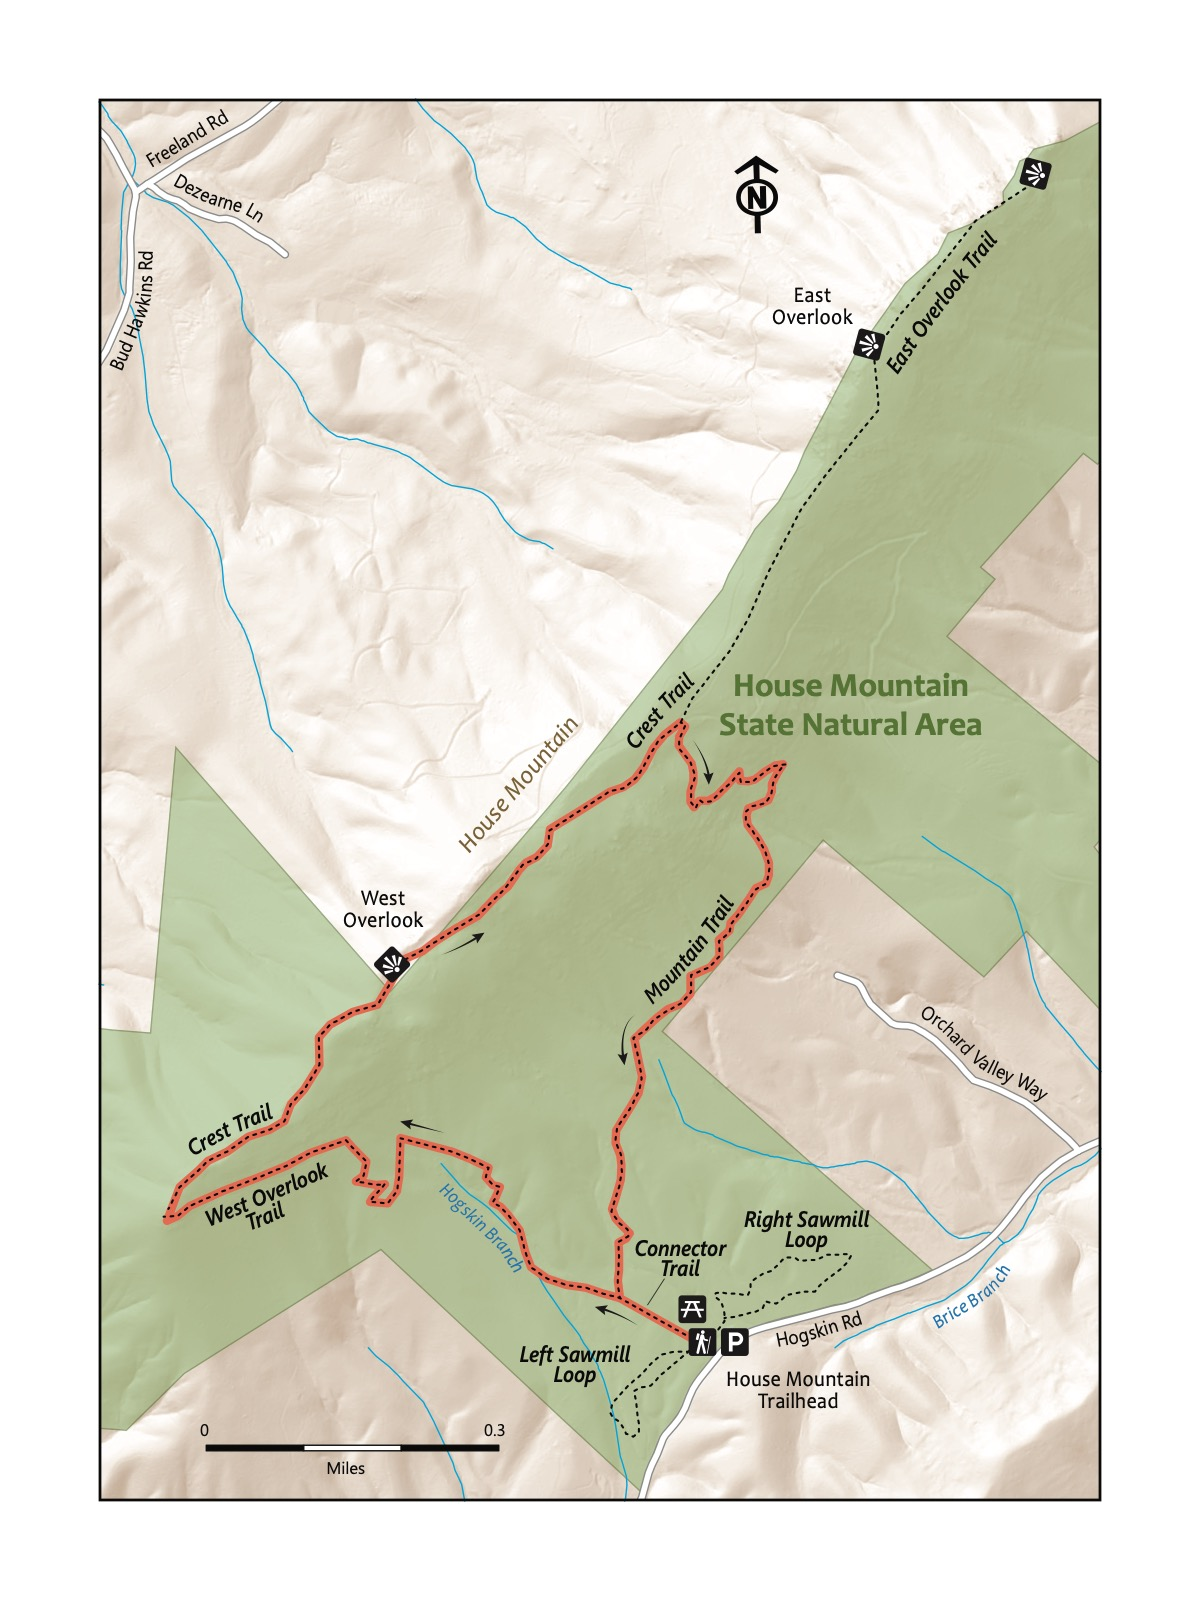
\includegraphics[keepaspectratio]{maps/trail-12-map.jpeg}}

\subsection{Directions to the
Trailhead}\label{directions-to-the-trailhead-11}

Trailhead Address: House Mountain Parking and Trailhead, 463P+WV
Corryton, Tennessee

Trailhead GPS Coordinates: 36.10483, -83.76276

Park at the large parking area and look for the large covered picnic
area. The Connector Trail near the picnic area tis where you'll begin
the hike.

\begin{tcolorbox}[enhanced jigsaw, colback=white, colframe=quarto-callout-note-color-frame, breakable, opacityback=0, toprule=.15mm, bottomrule=.15mm, rightrule=.15mm, left=2mm, leftrule=.75mm, arc=.35mm]
\begin{minipage}[t]{5.5mm}
\textcolor{quarto-callout-note-color}{\faInfo}
\end{minipage}%
\begin{minipage}[t]{\textwidth - 5.5mm}

\vspace{-3mm}\textbf{Pine Trees}\vspace{3mm}

A family of conifers recognizable by their needles, which usually grow
in bundles, and their seeds, which develop in stiff cones---making them
distinct from hemlocks, spruces, and firs.

\end{minipage}%
\end{tcolorbox}

\begin{figure}[H]

{\centering \pandocbounded{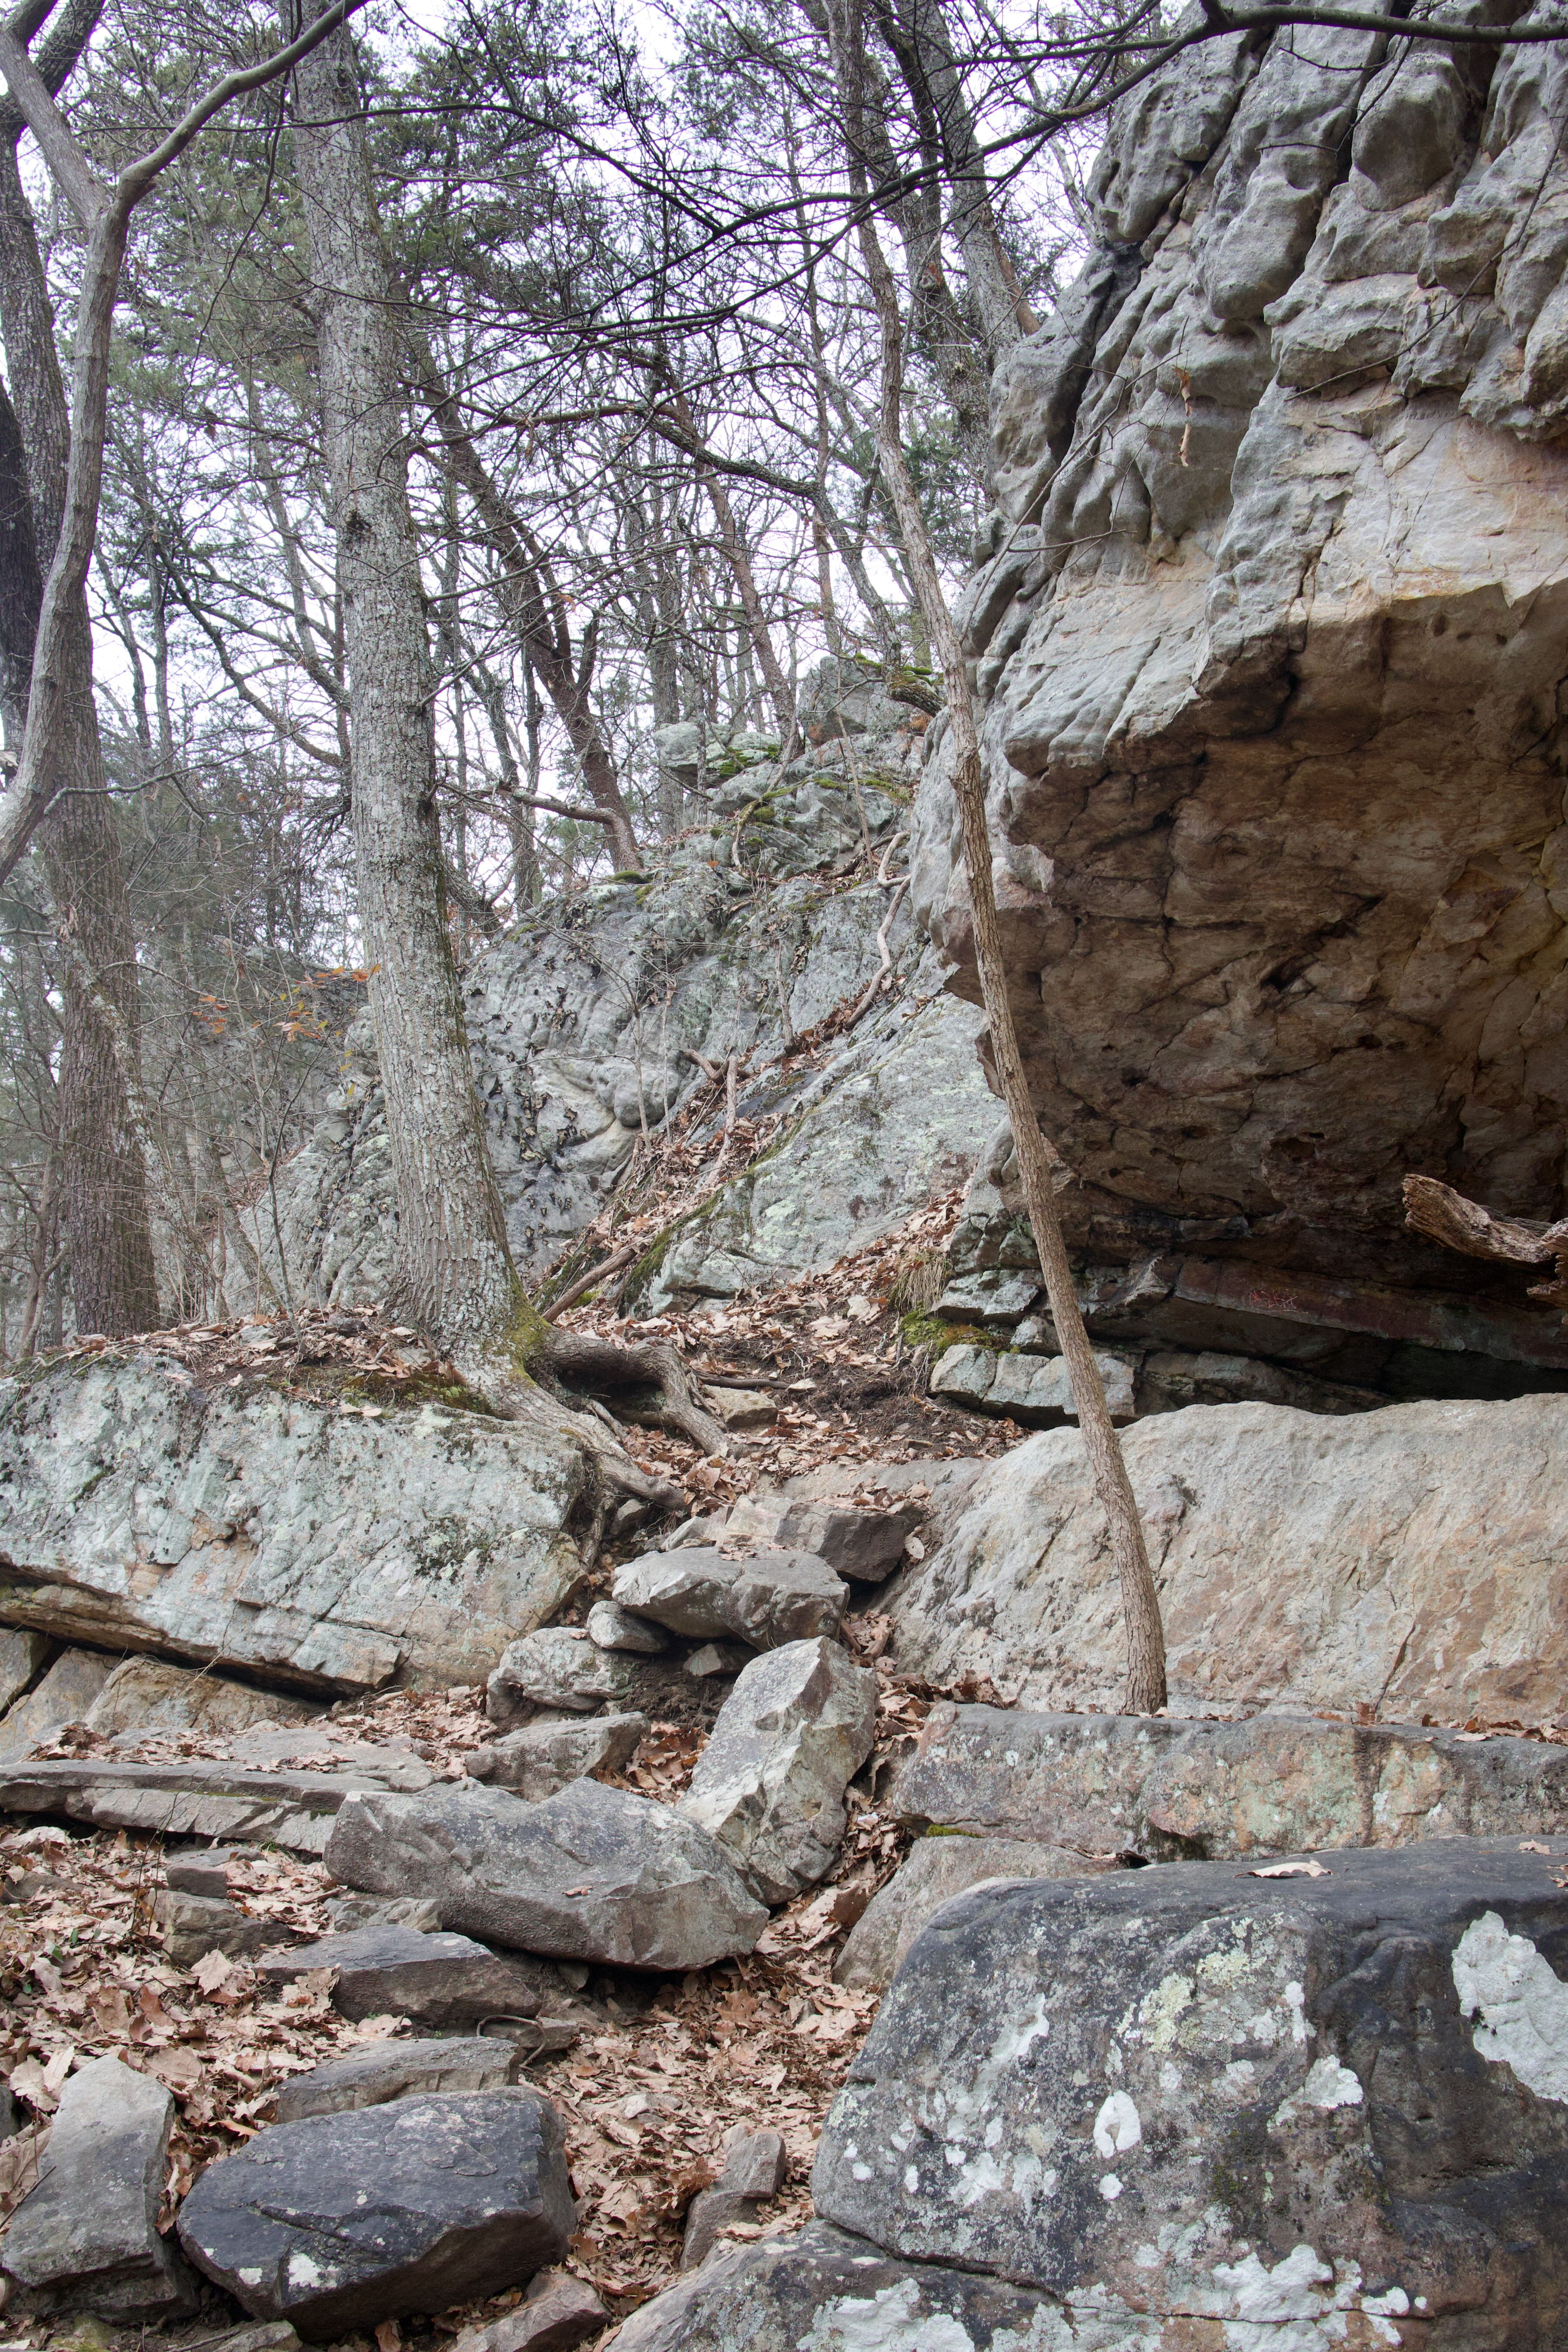
\includegraphics[keepaspectratio]{img/trail-12-figure-02.jpg}}

}

\caption{Photo credit to Katie and Joshua Rosenberg}

\end{figure}%

\subsection{Trail Description}\label{trail-description-11}

\begin{longtable}[]{@{}
  >{\raggedright\arraybackslash}p{(\linewidth - 2\tabcolsep) * \real{0.2639}}
  >{\raggedright\arraybackslash}p{(\linewidth - 2\tabcolsep) * \real{0.7361}}@{}}
\toprule\noalign{}
\begin{minipage}[b]{\linewidth}\raggedright
Distance from Start
\end{minipage} & \begin{minipage}[b]{\linewidth}\raggedright
Description
\end{minipage} \\
\midrule\noalign{}
\endhead
\bottomrule\noalign{}
\endlastfoot
0.0 & Start on the Connector Trail. \\
0.1 & Turn left onto the West Overlook Trail and begin your ascent. \\
0.85 & Rocky prominence. The trail changes here to the Crest Trail and
flattens. \\
1.25 & Reach the West Overlook. Continue on the Crest Trail. Optionally,
this is a suitable turn-around spot. \\
1.6 & Intersection with the East Overlook Trail. Turn right. \\
1.7 & Steep descent. \\
2.0 & Trail levels out, and the descent becomes more gradual and
winding. \\
2.3 & Trailhead. \\
\end{longtable}

\subsection{Nearby}\label{nearby-11}

\begin{itemize}
\tightlist
\item
  \textbf{Spend some time at Zoo Knoxville on the way home.} Zoo
  Knoxville (3500 Knoxville Zoo Dr, Knoxville, TN 37914) is accessible
  from I-40, on the way to House Mountain for those traveling from
  Knoxville or west of the city center, is a fantastic place to spend
  half a day (or longer)! It is one of our family's favorite spots.
\end{itemize}

\part{The Cumberland Plateau}

This region is the hidden gem near Knoxville. It's a plateau, with
valleys carved out by rivers through the softer sandstone rock that is
common in this area. There are also parts that are quite mountainous,
particularly near Frozen Head State Park.

The defining characteristic of the Cumberland Plateau is its geology:
incredible rock features and rock houses. You'll see rock formations
large and (striking) large on all of your hikes in the plateau. Some
will amaze you that they (and you) are in East Tennessee.

These seven hikes hikes are some of the most special to us in this book;
a little off-the-radar and even underappreciated, part of our motivation
for writing this book was to draw attention to them.

\pandocbounded{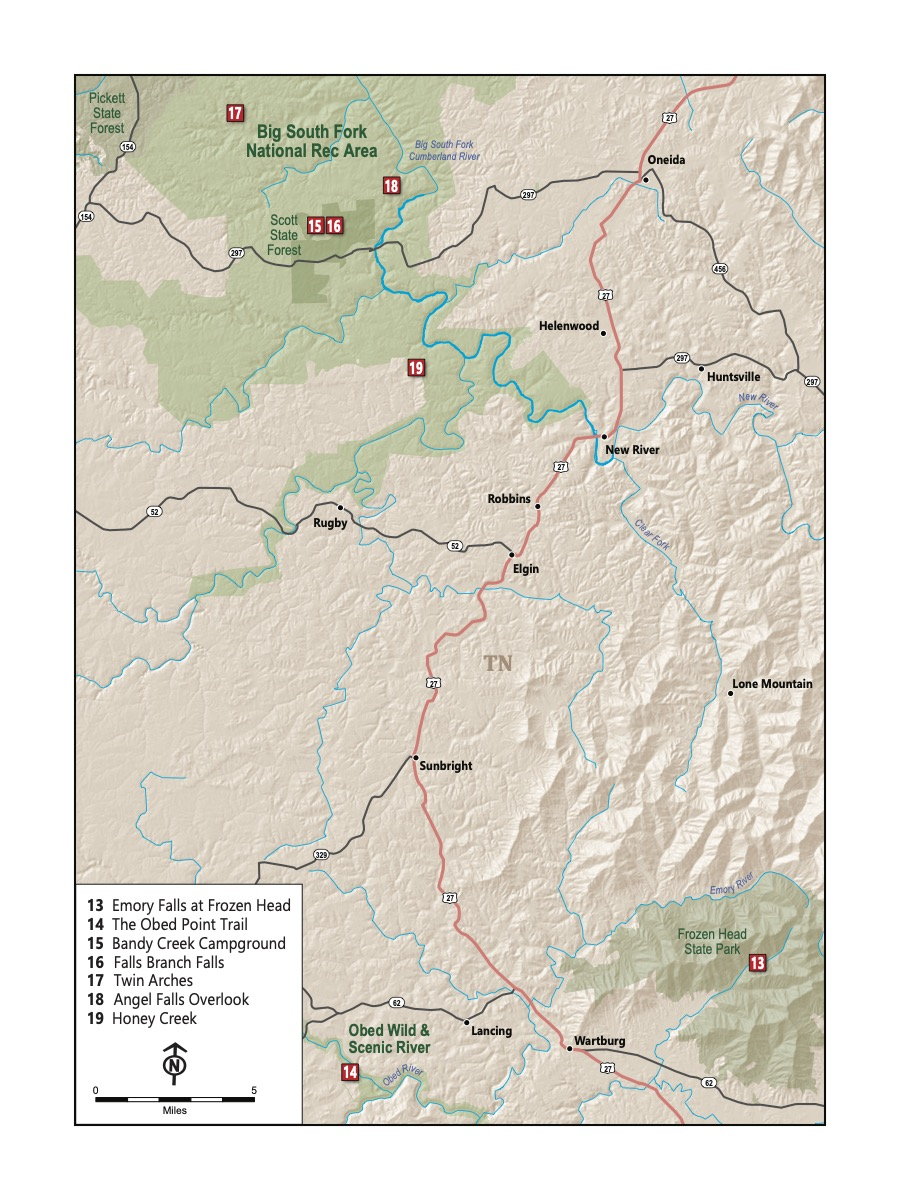
\includegraphics[keepaspectratio]{maps/plateau-region.jpg}}

\chapter{Trail 13: Emory Falls at Frozen
Head}\label{trail-13-emory-falls-at-frozen-head}

\subsection{Overview}\label{overview-13}

Writing about this trail makes us smile. In many ways, it's the perfect
kid hike! It starts at a beautiful trailhead along a pretty creek in the
deep woods. It gradually climbs before stopping at one of two scenic
waterfall, DeBord Falls, and is a perfectly acceptable place to turn
around with younger kids (we have many times!). It continues further to
Emory Falls before returning on a gradual slope back to the trailhead.
Stop at the playground you passed on the way to the trailhead beside the
same creek; the water is usually shallow enough to be perfect for
splashing and rock hopping. Please note, the trail is rocky, and your
kids will likely need reminders to slow down!

\begin{figure}[H]

{\centering \pandocbounded{\includegraphics[keepaspectratio]{img/trail-13-figure-01.jpg}}

}

\caption{Photo credit to Katie and Joshua Rosenberg}

\end{figure}%

\subsection{Key Characteristics}\label{key-characteristics-13}

\begin{longtable}[]{@{}
  >{\raggedright\arraybackslash}p{(\linewidth - 2\tabcolsep) * \real{0.1552}}
  >{\raggedright\arraybackslash}p{(\linewidth - 2\tabcolsep) * \real{0.8448}}@{}}
\toprule\noalign{}
\begin{minipage}[b]{\linewidth}\raggedright
\textbf{Characteristic}
\end{minipage} & \begin{minipage}[b]{\linewidth}\raggedright
\textbf{Details}
\end{minipage} \\
\midrule\noalign{}
\endhead
\bottomrule\noalign{}
\endlastfoot
Time Estimate & 2 hours - 3.5 hours \\
Trail Distance (Miles) & 2.4 \\
Elevation Change & Moderate \\
Pets & Allowed on leash \\
Parking Pass/Entrance Fee & Not Required \\
Restroom(s) & No restrooms at the trailhead parking, but you will pass
restrooms on the right about three quarters of a mile before the
trailhead parking area. \\
Best Ages & Little kids \\
Strollers and Wheelchairs & Not accessible \\
\end{longtable}

\pandocbounded{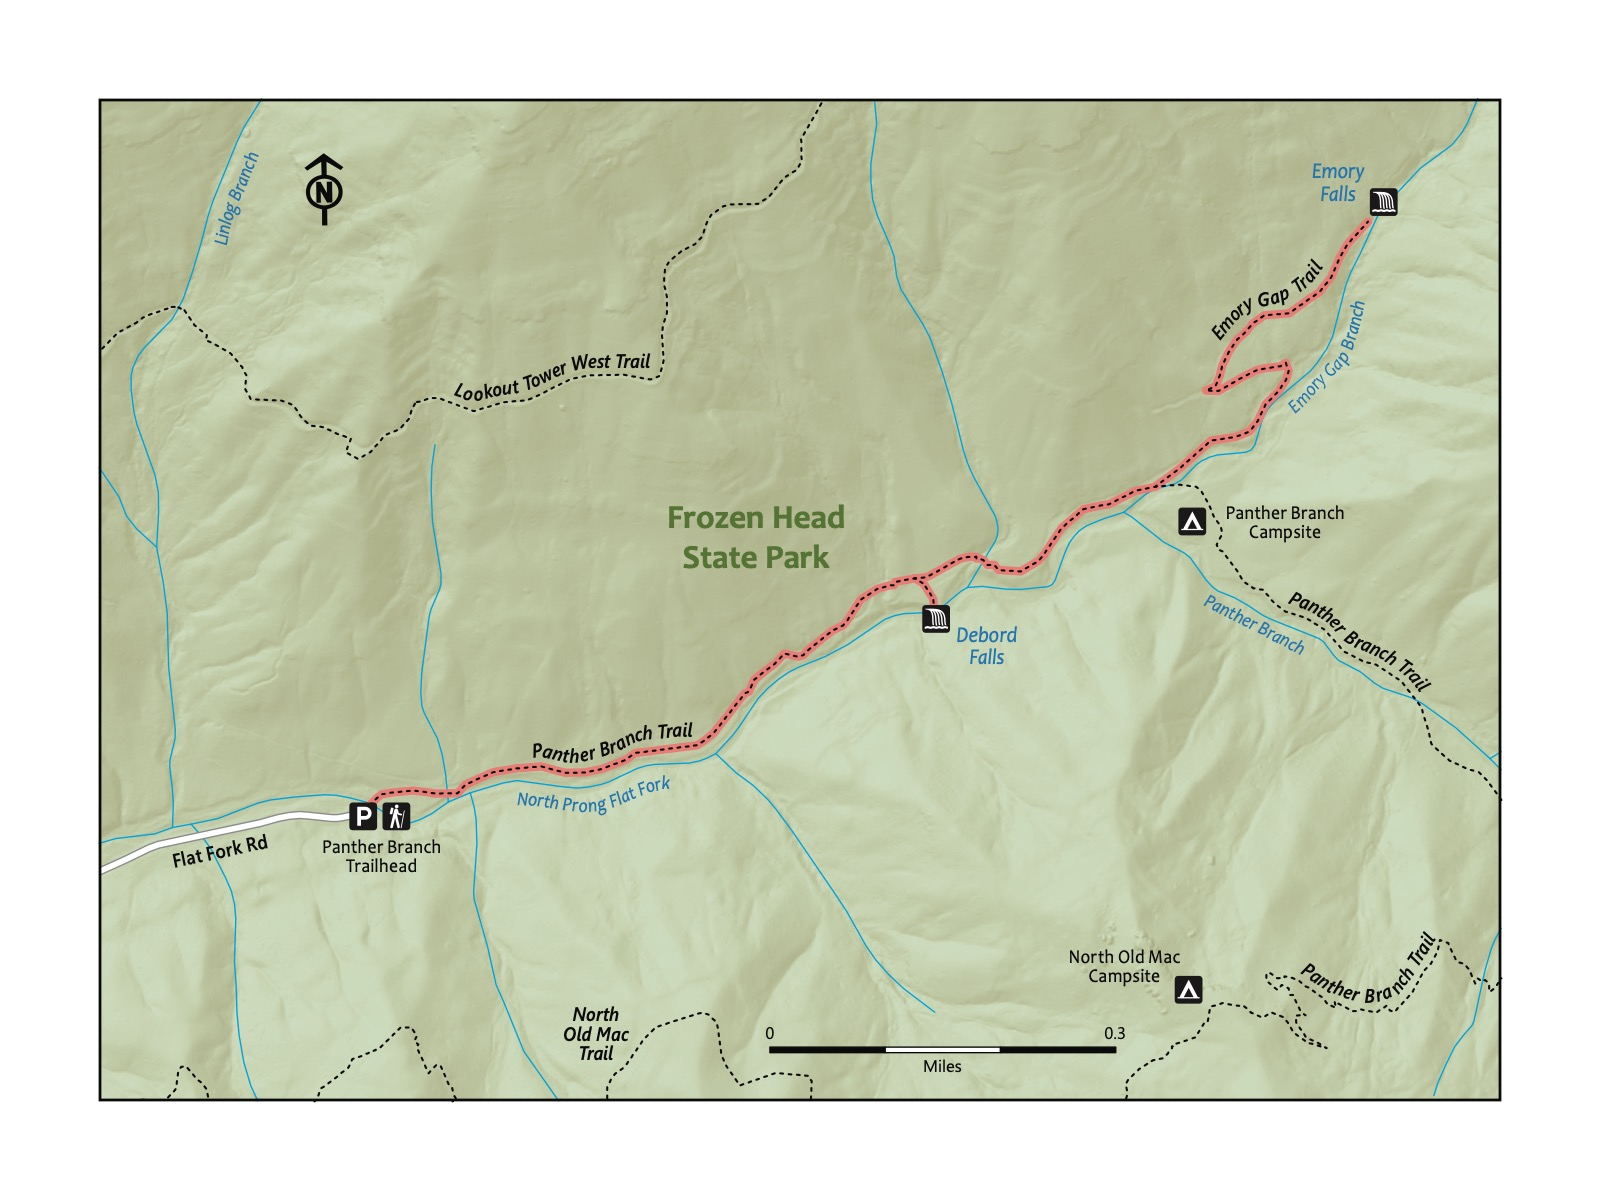
\includegraphics[keepaspectratio]{maps/trail-13-map.jpeg}}

\subsection{Directions to the
Trailhead}\label{directions-to-the-trailhead-12}

Trailhead Address: Emory Gap Trailhead, 4GP6+MV, Wartburg, TN 37887

Trailhead GPS Coordinates: 36.13658, -84.48785

Park at the Emory Gap Trailhead. Note that the above address uses a
``Plus code'' that will only work in Google Maps---because Emory Gap
Trailhead does not have a street address.

\begin{tcolorbox}[enhanced jigsaw, colback=white, colframe=quarto-callout-note-color-frame, breakable, opacityback=0, toprule=.15mm, bottomrule=.15mm, rightrule=.15mm, left=2mm, leftrule=.75mm, arc=.35mm]
\begin{minipage}[t]{5.5mm}
\textcolor{quarto-callout-note-color}{\faInfo}
\end{minipage}%
\begin{minipage}[t]{\textwidth - 5.5mm}

\vspace{-3mm}\textbf{Brushy Mountain State Penitentiary}\vspace{3mm}

A closed prison near Frozen Head State Park is full of lore due to its
remote location. Part of the inspiration for the Barkley Marathons
(you'll have to look it up). Now the site of a restaurant and
distillery.

\end{minipage}%
\end{tcolorbox}

\subsection{Trail Description}\label{trail-description-12}

\begin{longtable}[]{@{}
  >{\raggedright\arraybackslash}p{(\linewidth - 2\tabcolsep) * \real{0.1511}}
  >{\raggedright\arraybackslash}p{(\linewidth - 2\tabcolsep) * \real{0.8489}}@{}}
\toprule\noalign{}
\begin{minipage}[b]{\linewidth}\raggedright
Distance from Start
\end{minipage} & \begin{minipage}[b]{\linewidth}\raggedright
Description
\end{minipage} \\
\midrule\noalign{}
\endhead
\bottomrule\noalign{}
\endlastfoot
0.0 & Start by walking across the bridge at the trailhead. \\
0.55 & DeBord Falls. Walk down the (steep!) stairs on the right to view
the waterfall from below. Optional turnaround spot. \\
0.9 & Trail switchbacks. \\
1.1 & Steep and rocky section at the end to the viewing spot for Emory
Falls. \\
1.2 & After viewing the waterfall, head back to the start! \\
2.4 & Trailhead. \\
\end{longtable}

\begin{figure}[H]

{\centering \pandocbounded{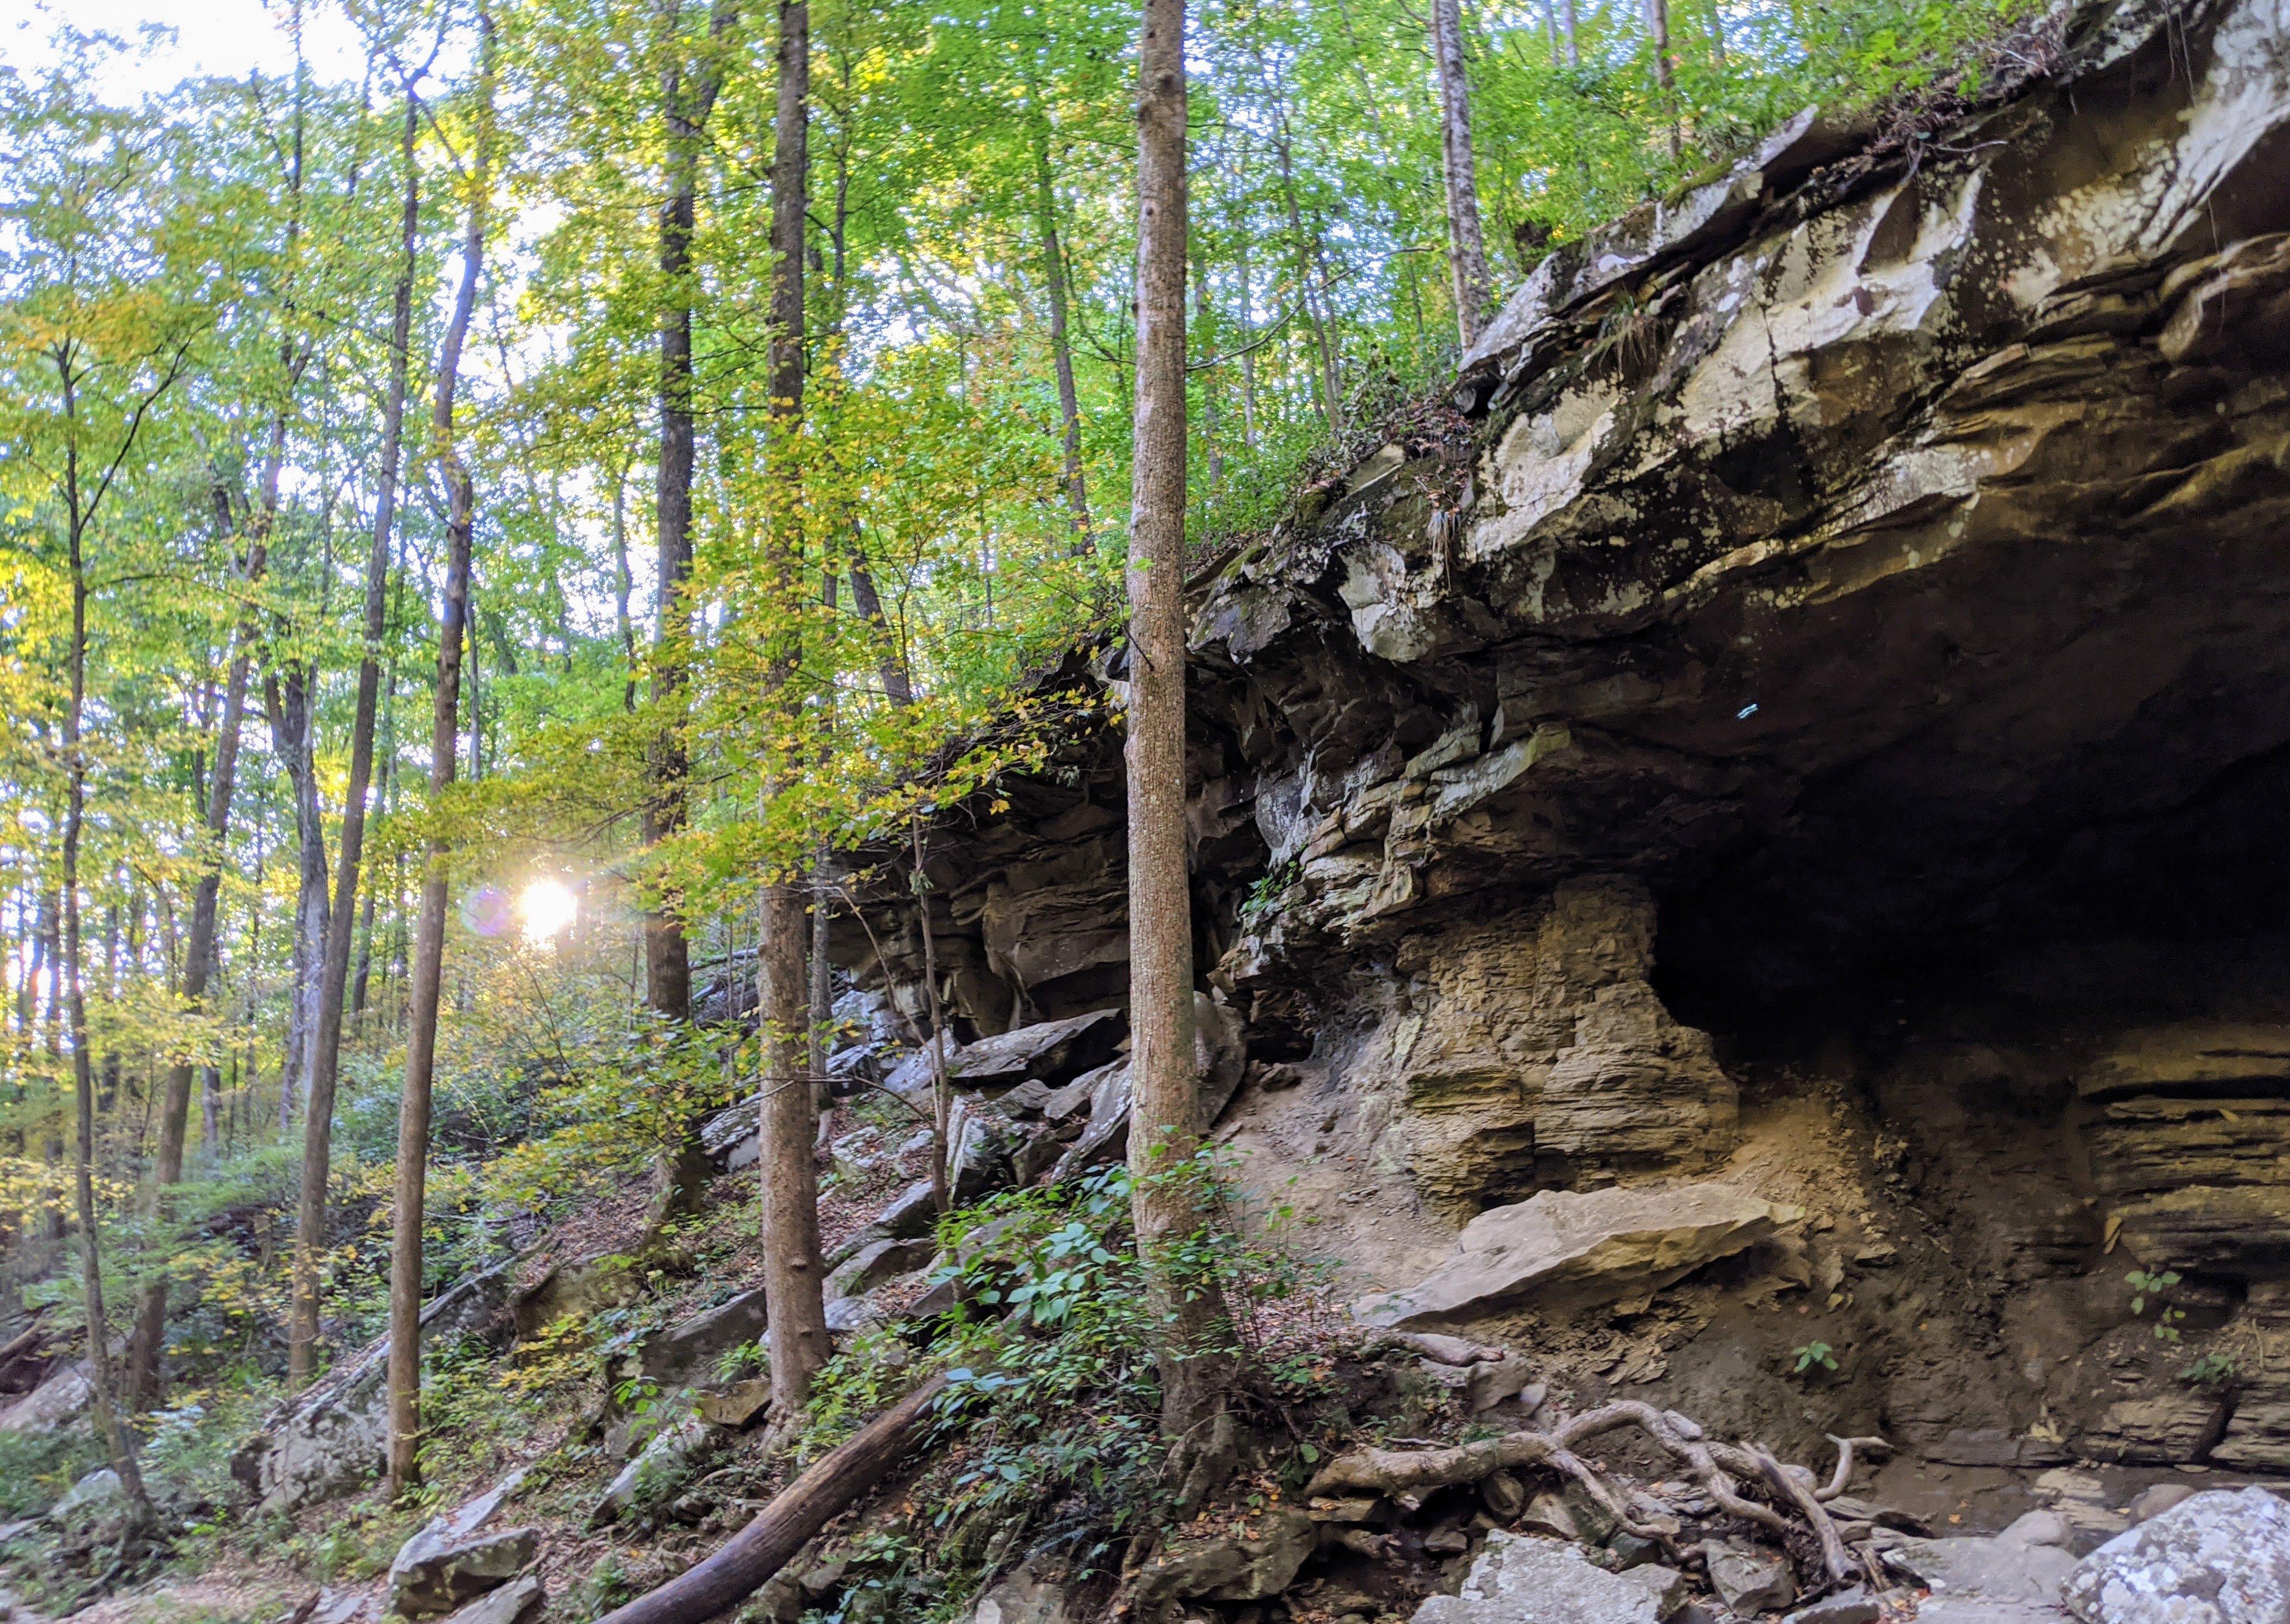
\includegraphics[keepaspectratio]{img/cliffs emory.jpg}}

}

\caption{Photo credit to Katie and Joshua Rosenberg}

\end{figure}%

\subsection{Nearby}\label{nearby-12}

\begin{itemize}
\tightlist
\item
  \textbf{Enjoy the playground!} There is a fun, shaded creekside
  playground 0.7 miles down the road from the trailhead. Most of the
  year, the creek is a perfect depth for safe splashing.
\item
  \textbf{Check out the Flat Fork Story Book Trail.} Starting near the
  playground, this short trail is great for the littlest hikers.
\item
  \textbf{Hike to the Frozen Head Mountain Summit.} A challenge for the
  biggest kid hikers and adults! This hike is around seven strenuous
  miles to and back from the Lookout Tower at the summit of Frozen Head
  Mountain, from which views of the Smokies far in the distance can be
  faintly visible on clear days.
\end{itemize}

\chapter{Trail 14: Obed Point Trail}\label{trail-14-obed-point-trail}

\subsection{Overview}\label{overview-14}

Just far enough to be off the radar of many in Knoxville, this trail has
a bit of everything - fun bridge crossings, deep forest, waterfalls, and
two pretty overlooks. It does not climb so much as to become tiresome,
but it's long enough to feel like a real adventure. There's something
about the Obed area that feels both wild and inviting. The only
downside? It's a little out-of-the-way; in some ways, this trail feels
farther than some destinations in the Smokies. It's worth it for a great
family hike with kids of all ages. Though out of the way, there are a
few fun things to do to extend the hike or to visit very nearby on the
way home. Great for kids of all hiking ages, and not a bad hike on which
to carry a little one.

\begin{figure}[H]

{\centering \pandocbounded{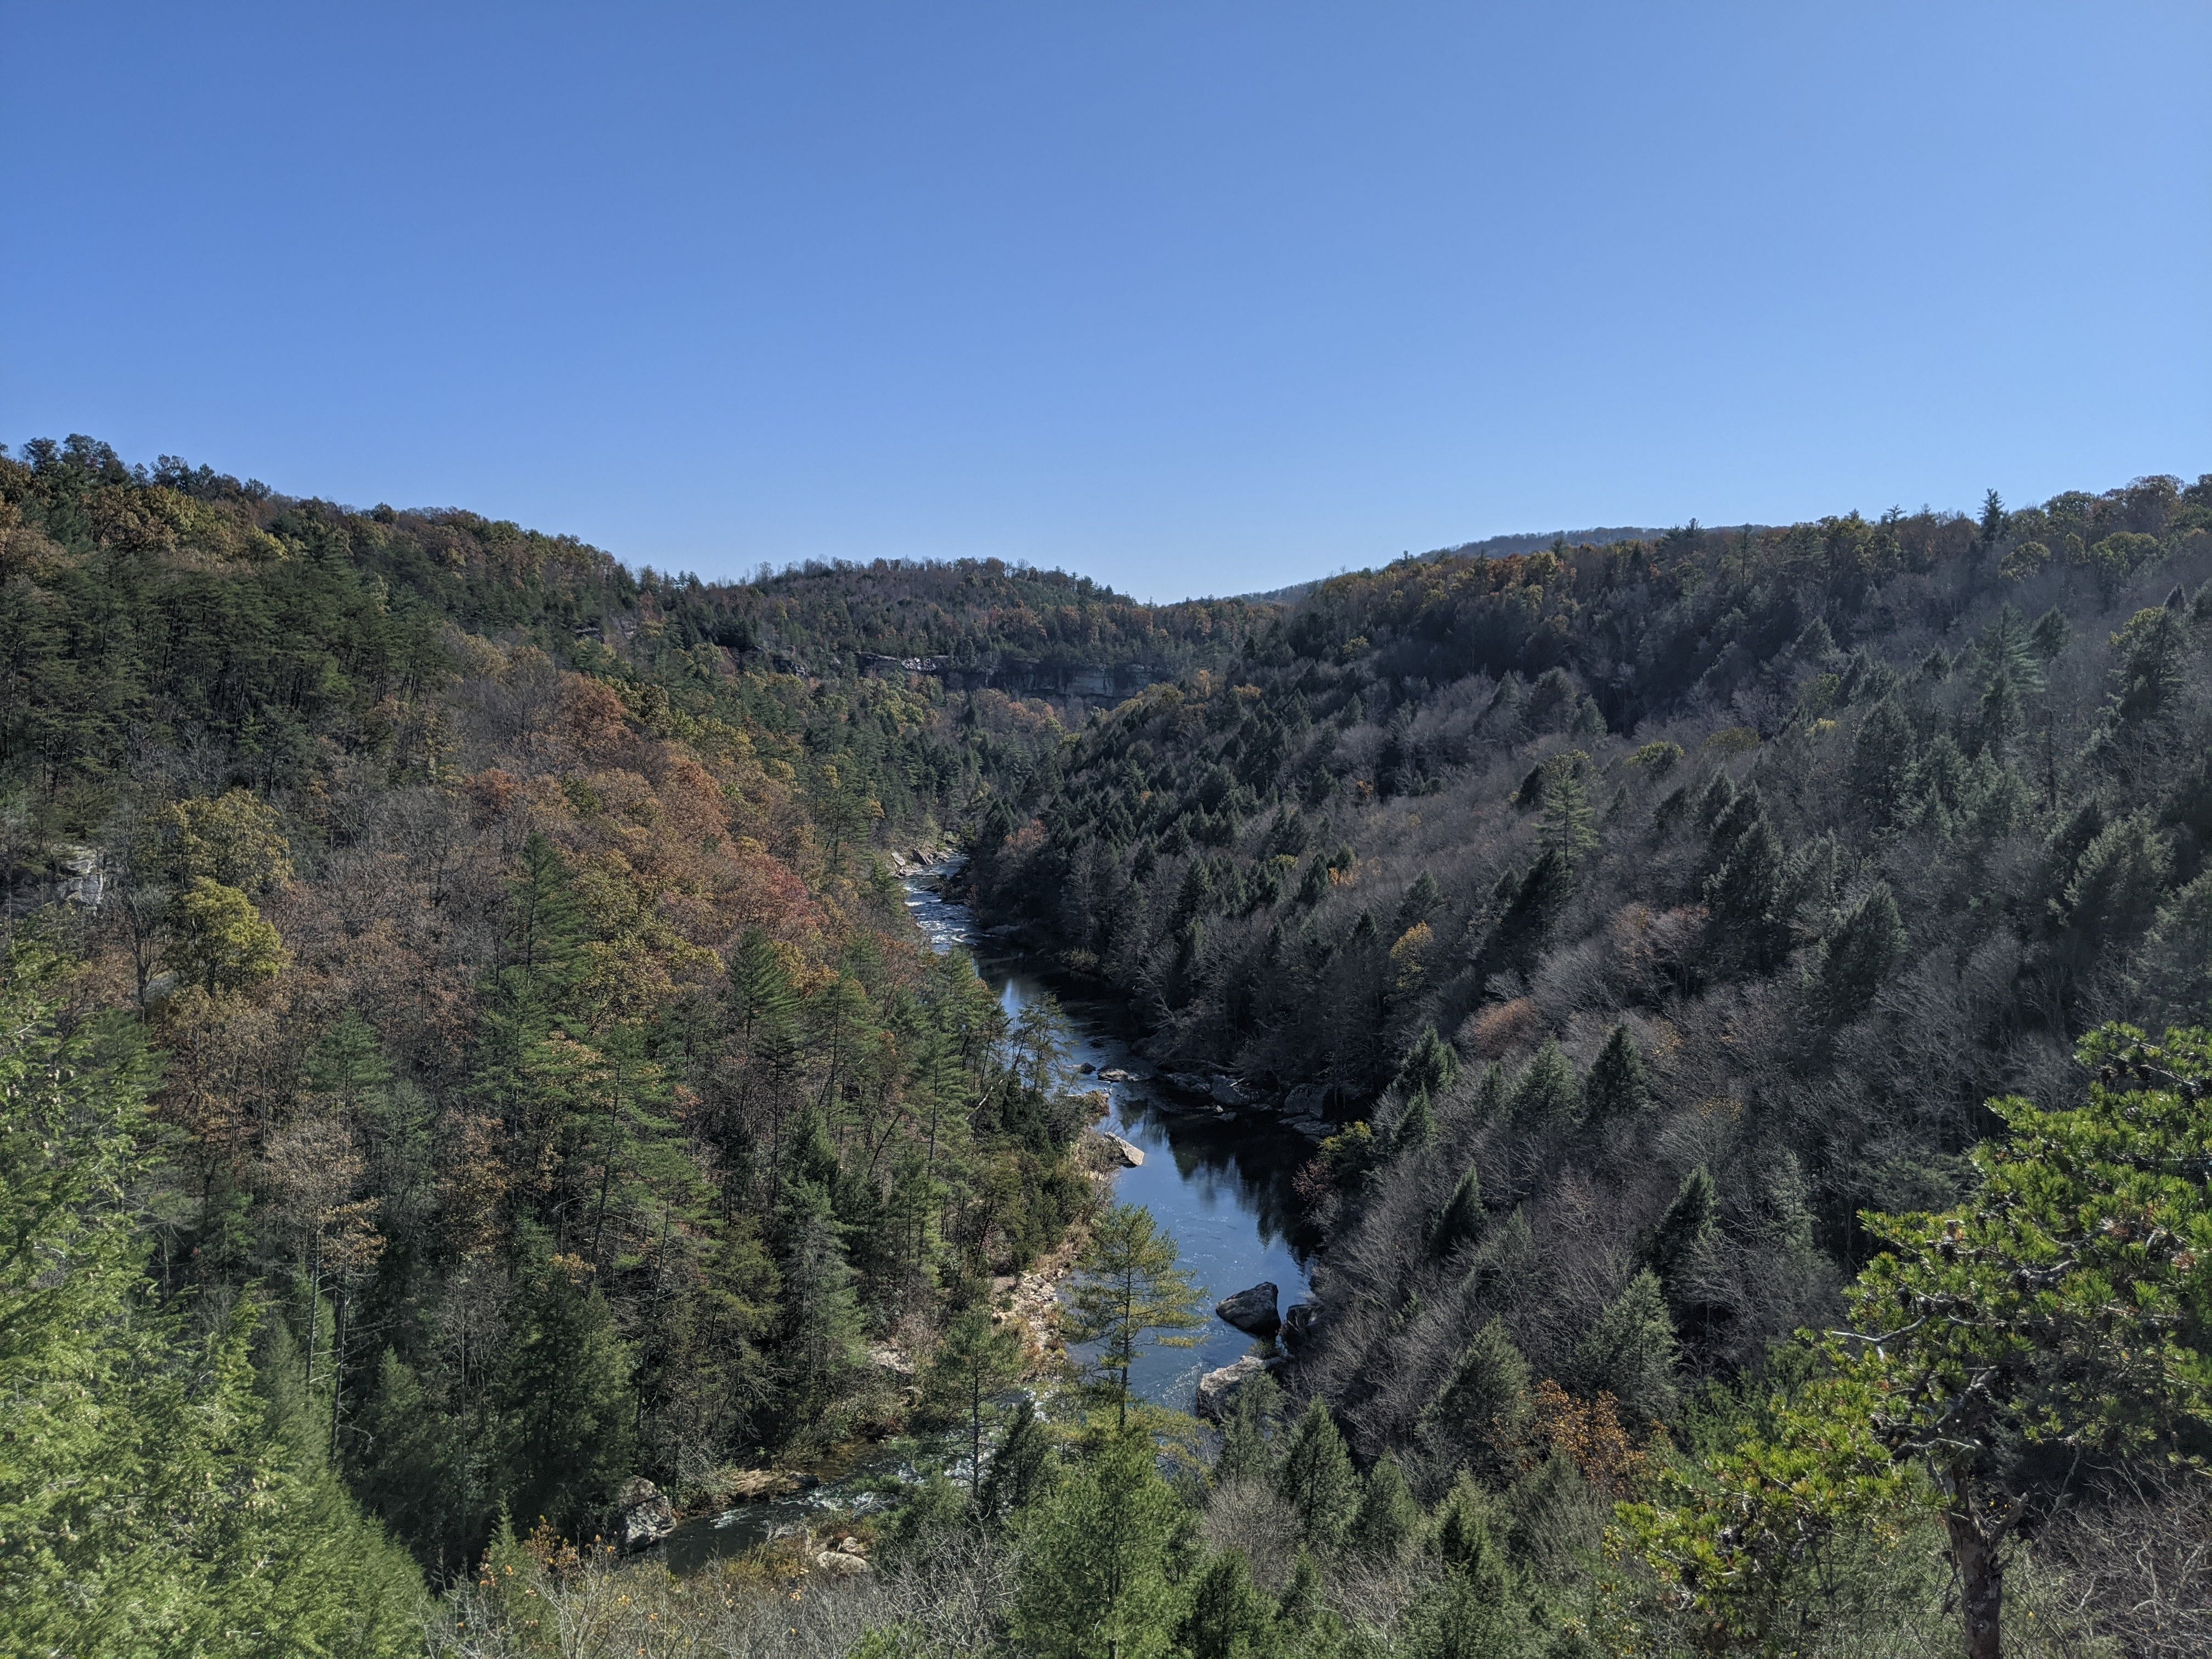
\includegraphics[keepaspectratio]{img/trail-14-figure-01.jpg}}

}

\caption{Photo credit to Katie and Joshua Rosenberg}

\end{figure}%

\subsection{Key Characteristics}\label{key-characteristics-14}

\begin{longtable}[]{@{}
  >{\raggedright\arraybackslash}p{(\linewidth - 2\tabcolsep) * \real{0.5400}}
  >{\raggedright\arraybackslash}p{(\linewidth - 2\tabcolsep) * \real{0.4600}}@{}}
\toprule\noalign{}
\begin{minipage}[b]{\linewidth}\raggedright
\textbf{Characteristic}
\end{minipage} & \begin{minipage}[b]{\linewidth}\raggedright
\textbf{Details}
\end{minipage} \\
\midrule\noalign{}
\endhead
\bottomrule\noalign{}
\endlastfoot
Time Estimate & 2.5 hours - 4.5 hours \\
Trail Distance (Miles) & 3.6 \\
Elevation Change & Gentle \\
Pets & Allowed on leash \\
Parking Pass/Entrance Fee & Not Required \\
Restroom(s) & Yes \\
Best Ages & Little kids and Big kids \\
Strollers and Wheelchairs & Not accessible \\
\end{longtable}

\pandocbounded{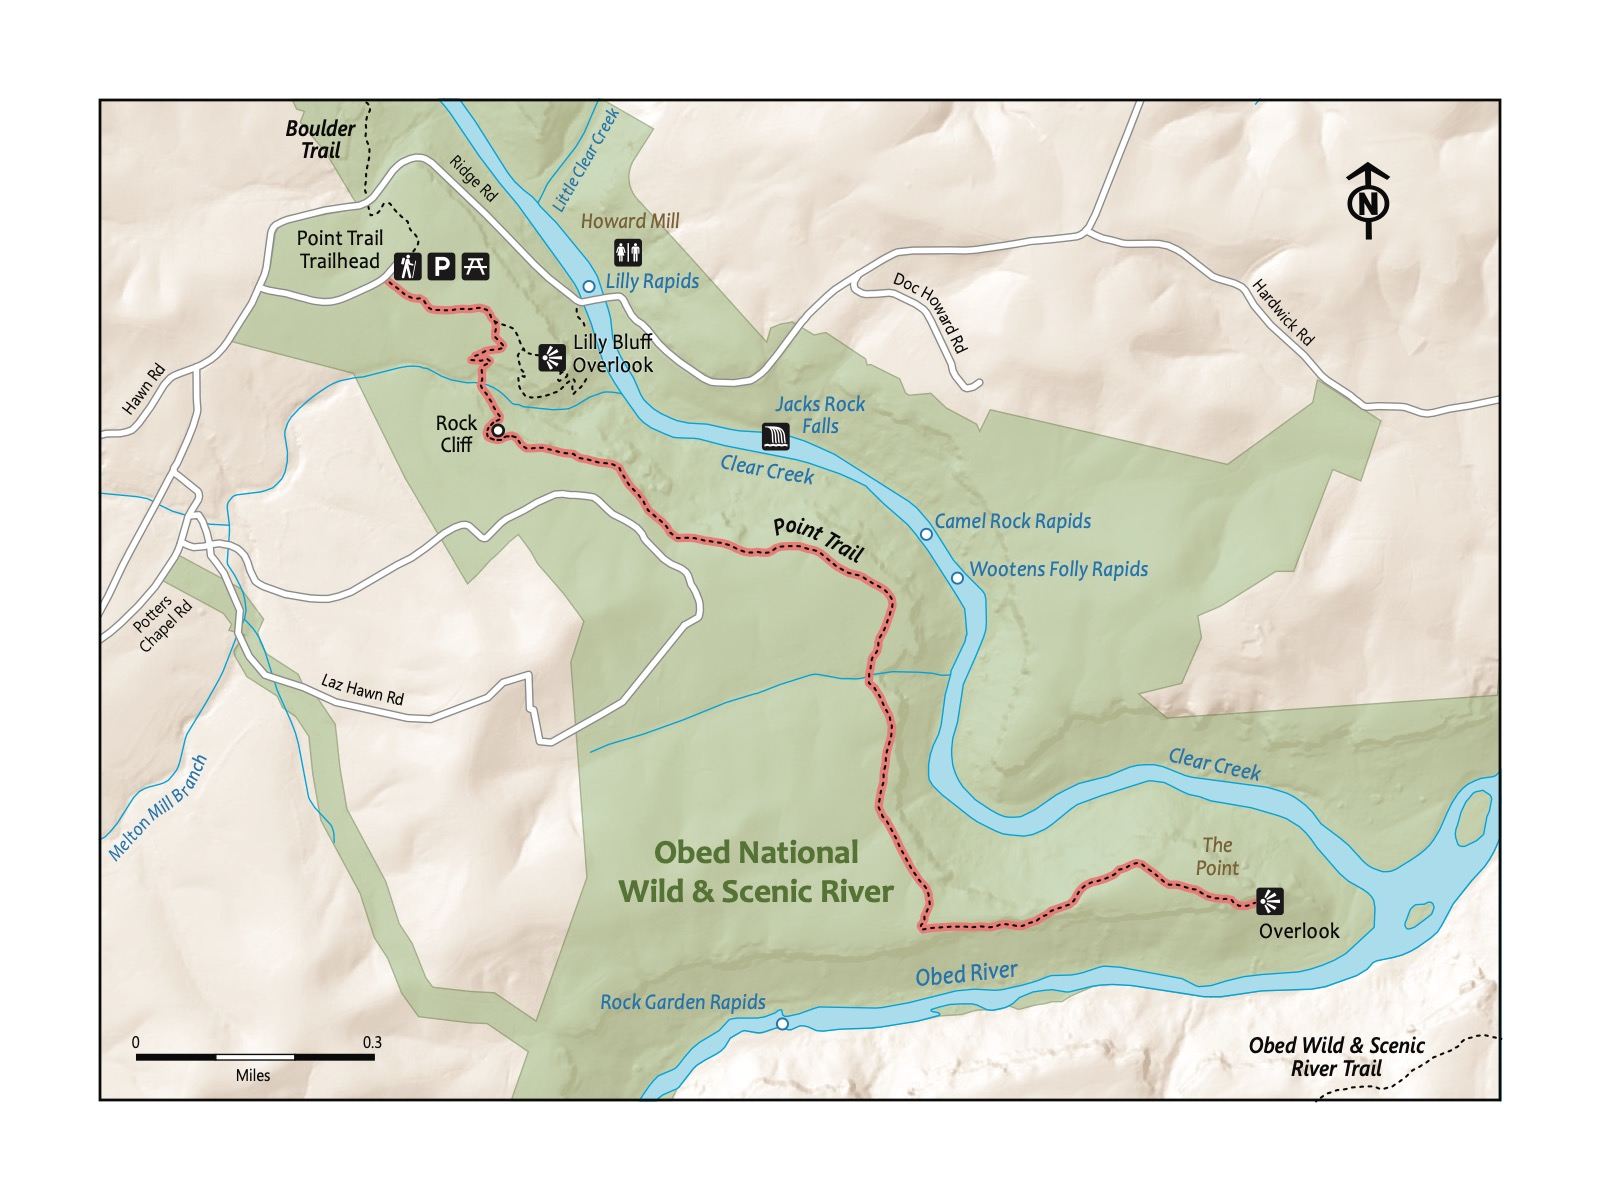
\includegraphics[keepaspectratio]{maps/trail-14-map.jpeg}}

\subsection{Directions to the
Trailhead}\label{directions-to-the-trailhead-13}

Trailhead Address: Lilly Bluff Trailhead, 1 Lilly Bluff Trail Head,
Lancing, TN 37770

Trailhead GPS Coordinates: 36.10239, -84.72183

The above address should easily navigate you to the large parking area
with a restroom. Look for the sign for the point trail.

\subsection{Trail Description}\label{trail-description-13}

\begin{longtable}[]{@{}
  >{\raggedright\arraybackslash}p{(\linewidth - 2\tabcolsep) * \real{0.2917}}
  >{\raggedright\arraybackslash}p{(\linewidth - 2\tabcolsep) * \real{0.7083}}@{}}
\toprule\noalign{}
\begin{minipage}[b]{\linewidth}\raggedright
Distance from Start
\end{minipage} & \begin{minipage}[b]{\linewidth}\raggedright
Description
\end{minipage} \\
\midrule\noalign{}
\endhead
\bottomrule\noalign{}
\endlastfoot
0.0 & Start on the Point Trail. \\
0.15 & Side trail to the Lilly Bluff Overlook for Clear Creek (we
recommend!). \\
0.4 & Small bridge crossing. \\
0.45 & Large boulders and a rock wall. The trail winds around the side
and atop the back of the wall. \\
0.5 & Trail flattens and winds along the side of a ridge. \\
1 & Trail bends to the right. \\
1.4 & Trail bends to the left. \\
1.8 & Overlook of the juncture of Clear Creek and Obed River. There are
many great spots to view the rivers! After a good rest, turn around and
head back to the trailhead. \\
3.6 & Trailhead. \\
\end{longtable}

\begin{figure}[H]

{\centering \pandocbounded{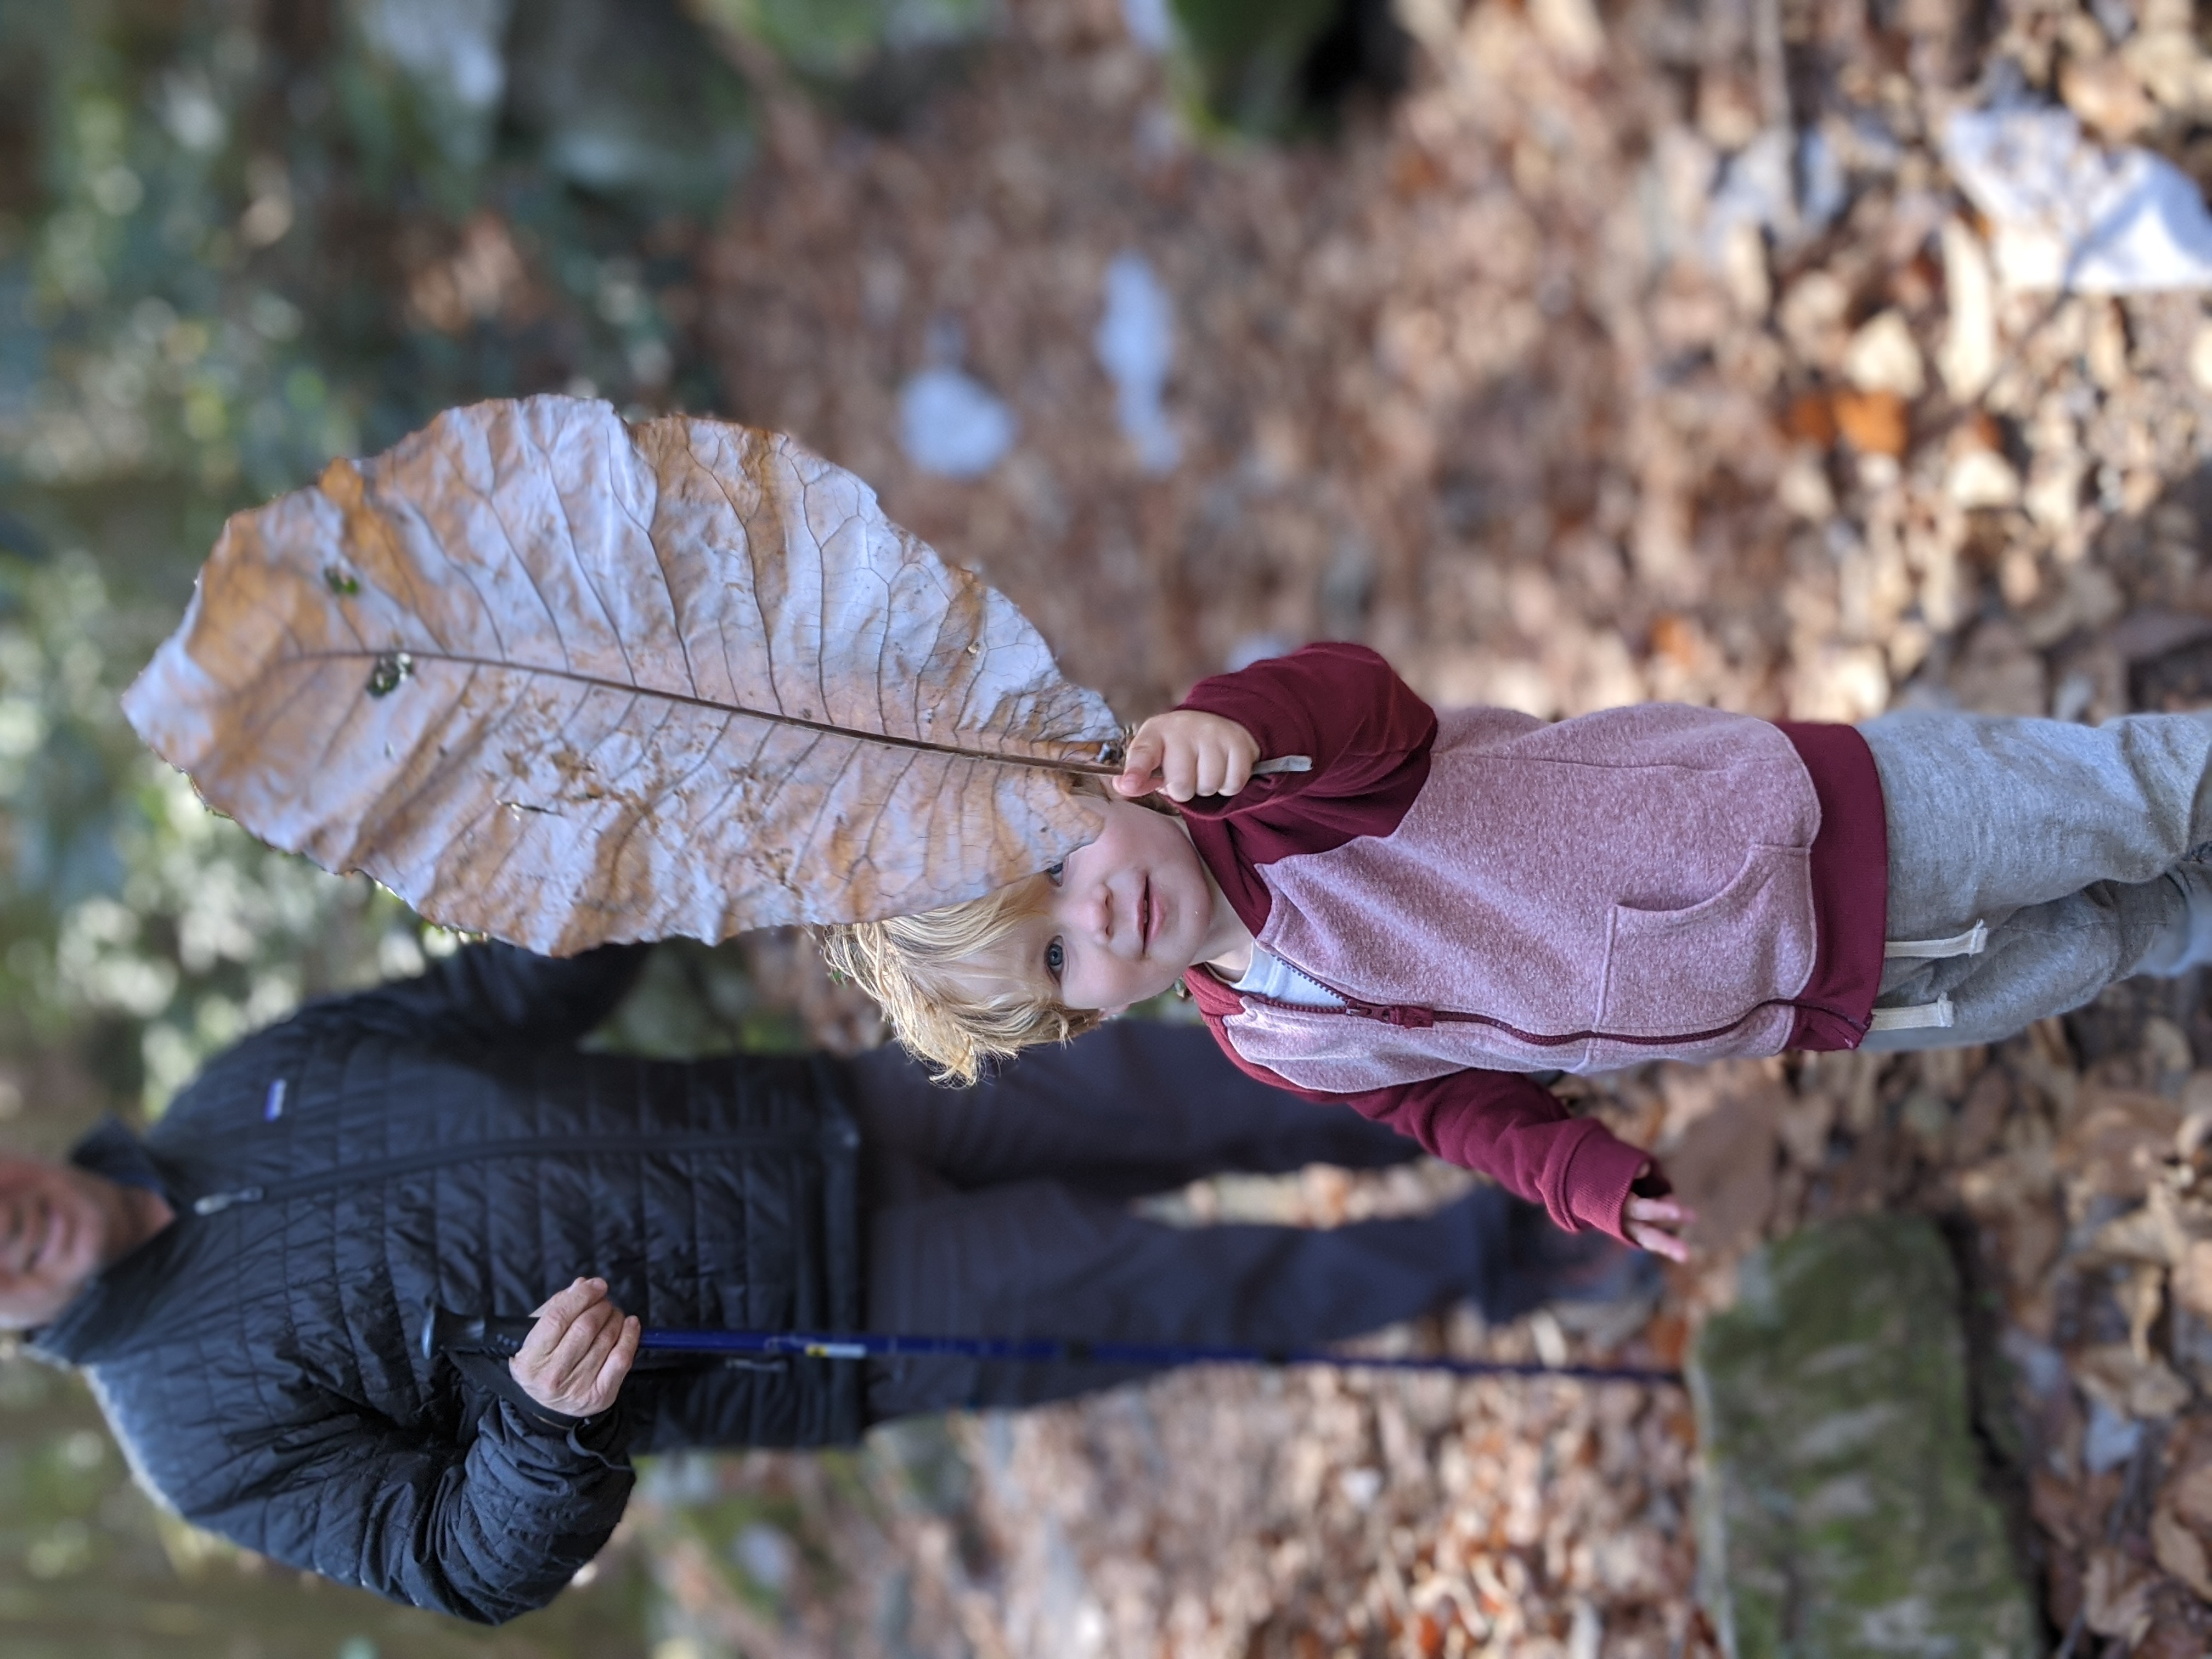
\includegraphics[keepaspectratio]{img/bigleaf magnolia.jpg}}

}

\caption{Photo credit to Katie and Joshua Rosenberg}

\end{figure}%

\begin{tcolorbox}[enhanced jigsaw, colback=white, colframe=quarto-callout-note-color-frame, breakable, opacityback=0, toprule=.15mm, bottomrule=.15mm, rightrule=.15mm, left=2mm, leftrule=.75mm, arc=.35mm]
\begin{minipage}[t]{5.5mm}
\textcolor{quarto-callout-note-color}{\faInfo}
\end{minipage}%
\begin{minipage}[t]{\textwidth - 5.5mm}

\vspace{-3mm}\textbf{Bigleaf Magnolia}\vspace{3mm}

This tree has the largest simple leaf of any North American tree---one
single, undivided leaf! In the fall, its leaves scatter across the
ground like pages from a newspaper. You'll find it common on the
Cumberland Plateau, though it's rare in the Smokies.

\end{minipage}%
\end{tcolorbox}

\subsection{Nearby}\label{nearby-13}

\begin{itemize}
\tightlist
\item
  Hang out at Lilly Pad Hopyard Brewery, only open Saturdays and
  Sundays, 12-6 p.m. The Lilly Pad Hopyard Brewery
  (\url{https://www.lillypadhopyardbrewery.com}) is a surprising,
  fantastic, kid-friendly destination for food and drinks.
\item
  Play around the bouldering area. The Trailhead features a nearby
  shaded area full of boulders. While we've often used this spot as a
  peaceful place to finish kiddo naps, older kids love trying to climb
  the boulders.
\end{itemize}

\chapter{Trail 15: Bandy Creek
Campground}\label{trail-15-bandy-creek-campground}

\subsection{Overview}\label{overview-15}

A welcoming, gentle introduction to the Big South Fork. This hike pairs
best with a stay at the campground or if you're hiking the nearby Angel
Falls Trail or the Fall Branch Falls trails. This happens to be the
flattest trail in the book. While short, it's almost entirely on a dirt
path, making it a great hike for toddlers or little kids -- or parents
carrying babies in a carrier.

\subsection{Key Characteristics}\label{key-characteristics-15}

\begin{longtable}[]{@{}
  >{\raggedright\arraybackslash}p{(\linewidth - 2\tabcolsep) * \real{0.1508}}
  >{\raggedright\arraybackslash}p{(\linewidth - 2\tabcolsep) * \real{0.8492}}@{}}
\toprule\noalign{}
\begin{minipage}[b]{\linewidth}\raggedright
\textbf{Characteristic}
\end{minipage} & \begin{minipage}[b]{\linewidth}\raggedright
\textbf{Details}
\end{minipage} \\
\midrule\noalign{}
\endhead
\bottomrule\noalign{}
\endlastfoot
Time Estimate & 45 minutes - 1 hour, 15 minutes \%Just thought -- might
want to check if you do time like this, or if you abbreviate 1.25. Just
want to keep it uniform\% \\
Trail Distance (Miles) & 1.3 \\
Elevation Change & Flat \\
Pets & Allowed on leash \\
Parking Pass/Entrance Fee & Not Required \\
Restroom(s) & Yes \\
Best Ages & Toddlers and Little kids \\
Strollers and Wheelchairs & Not accessible \\
\end{longtable}

\pandocbounded{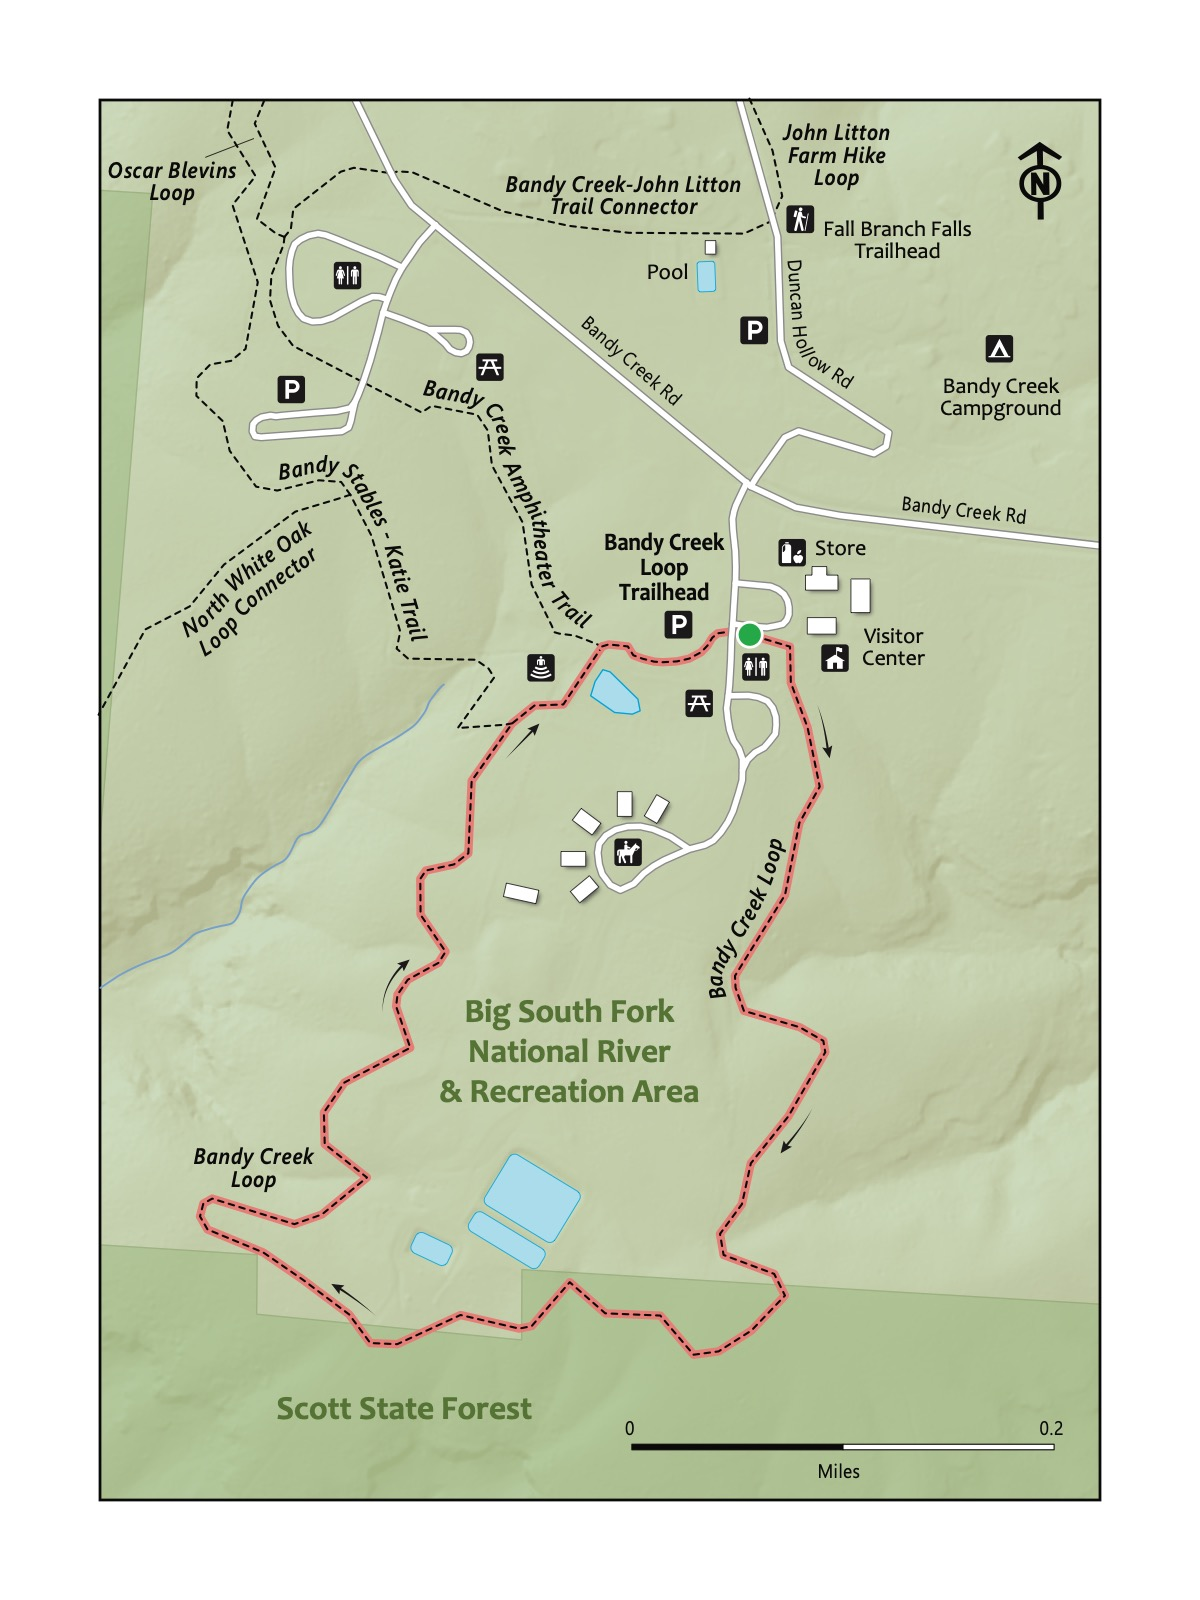
\includegraphics[keepaspectratio]{maps/trail-15-map.jpeg}}

\subsection{Directions to the
Trailhead}\label{directions-to-the-trailhead-14}

Trailhead Address: Bandy Creek Visitors Center, 151 Stable Rd, Oneida,
TN 37841

Trailhead GPS Coordinates: 36.49062, -84.69777

\begin{tcolorbox}[enhanced jigsaw, colback=white, colframe=quarto-callout-note-color-frame, breakable, opacityback=0, toprule=.15mm, bottomrule=.15mm, rightrule=.15mm, left=2mm, leftrule=.75mm, arc=.35mm]
\begin{minipage}[t]{5.5mm}
\textcolor{quarto-callout-note-color}{\faInfo}
\end{minipage}%
\begin{minipage}[t]{\textwidth - 5.5mm}

\vspace{-3mm}\textbf{Sandstone}\vspace{3mm}

The dominant rock on the Cumberland Plateau is sandstone---a relatively
soft rock that erosion has easily sculpted. Over time, its wearing has
carved cliffs, deep river valleys, and arches that characterize the
Cumberland Plateau.

\end{minipage}%
\end{tcolorbox}

The trailhead address will navigate you to the nearby Visitors Center
(worth a visit when open (9:00 am - 5:00 pm year-round!). From the
Visitors Center, look for the signs for the Bandy Creek Loop to begin
the hike.

\subsection{Trail Description}\label{trail-description-14}

\begin{longtable}[]{@{}
  >{\raggedright\arraybackslash}p{(\linewidth - 2\tabcolsep) * \real{0.1680}}
  >{\raggedright\arraybackslash}p{(\linewidth - 2\tabcolsep) * \real{0.8320}}@{}}
\toprule\noalign{}
\begin{minipage}[b]{\linewidth}\raggedright
Distance from Start
\end{minipage} & \begin{minipage}[b]{\linewidth}\raggedright
Description
\end{minipage} \\
\midrule\noalign{}
\endhead
\bottomrule\noalign{}
\endlastfoot
0.0 & Start on the Bandy Loop Trail. Wind gradually toward the horse
stables. \\
0.15 & Pass the horse stables on the right. There's an easy connector
trail to them near the end of the loop. \\
1.15 & Connector trail to the horse stables. \\
1.3 & Return to the parking area and trailhead. \\
\end{longtable}

\subsection{Nearby}\label{nearby-14}

\begin{itemize}
\tightlist
\item
  \textbf{Enjoy a visit at the horse stables.} Kids will likely love the
  nearby stables that often house many horses -- most from guests at the
  campground who will ride the nearby horse-friendly trails. The nearby
  Bandy Creek Loop trail is also a good, short hike for young kiddos.
\item
  \textbf{Camp at Bandy Creek.} This is a large, modern, scenic
  campground, very much worth a visit, though it is off-the-radar of
  many. You can almost always find a spot here---even on holiday
  weekends.
\item
  \textbf{Hike the Fall Branch Falls or Angel Falls trails.} See those
  chapters for more details.
\end{itemize}

\chapter{Trail 16: Fall Branch Falls}\label{trail-16-fall-branch-falls}

\subsection{Overview}\label{overview-16}

This hike is a perfect counterbalance to the wonderful but far more
familiar Great Smoky Mountains National Park. This hike, like the Big
South Fork, is quieter and subtler than the Smokies. It features unique
rock cliffs that are perfect for kids to take in and explore. The
visitor center, horse stables (not to mention hundreds of miles of
nearby trails), complement the hike. Because you can turn around at any
point, this hike is great for kids of nearly any age. However, be aware
of the ladders along the hike that can be a little tricky for the
youngest kids to navigate!

\begin{figure}[H]

{\centering \pandocbounded{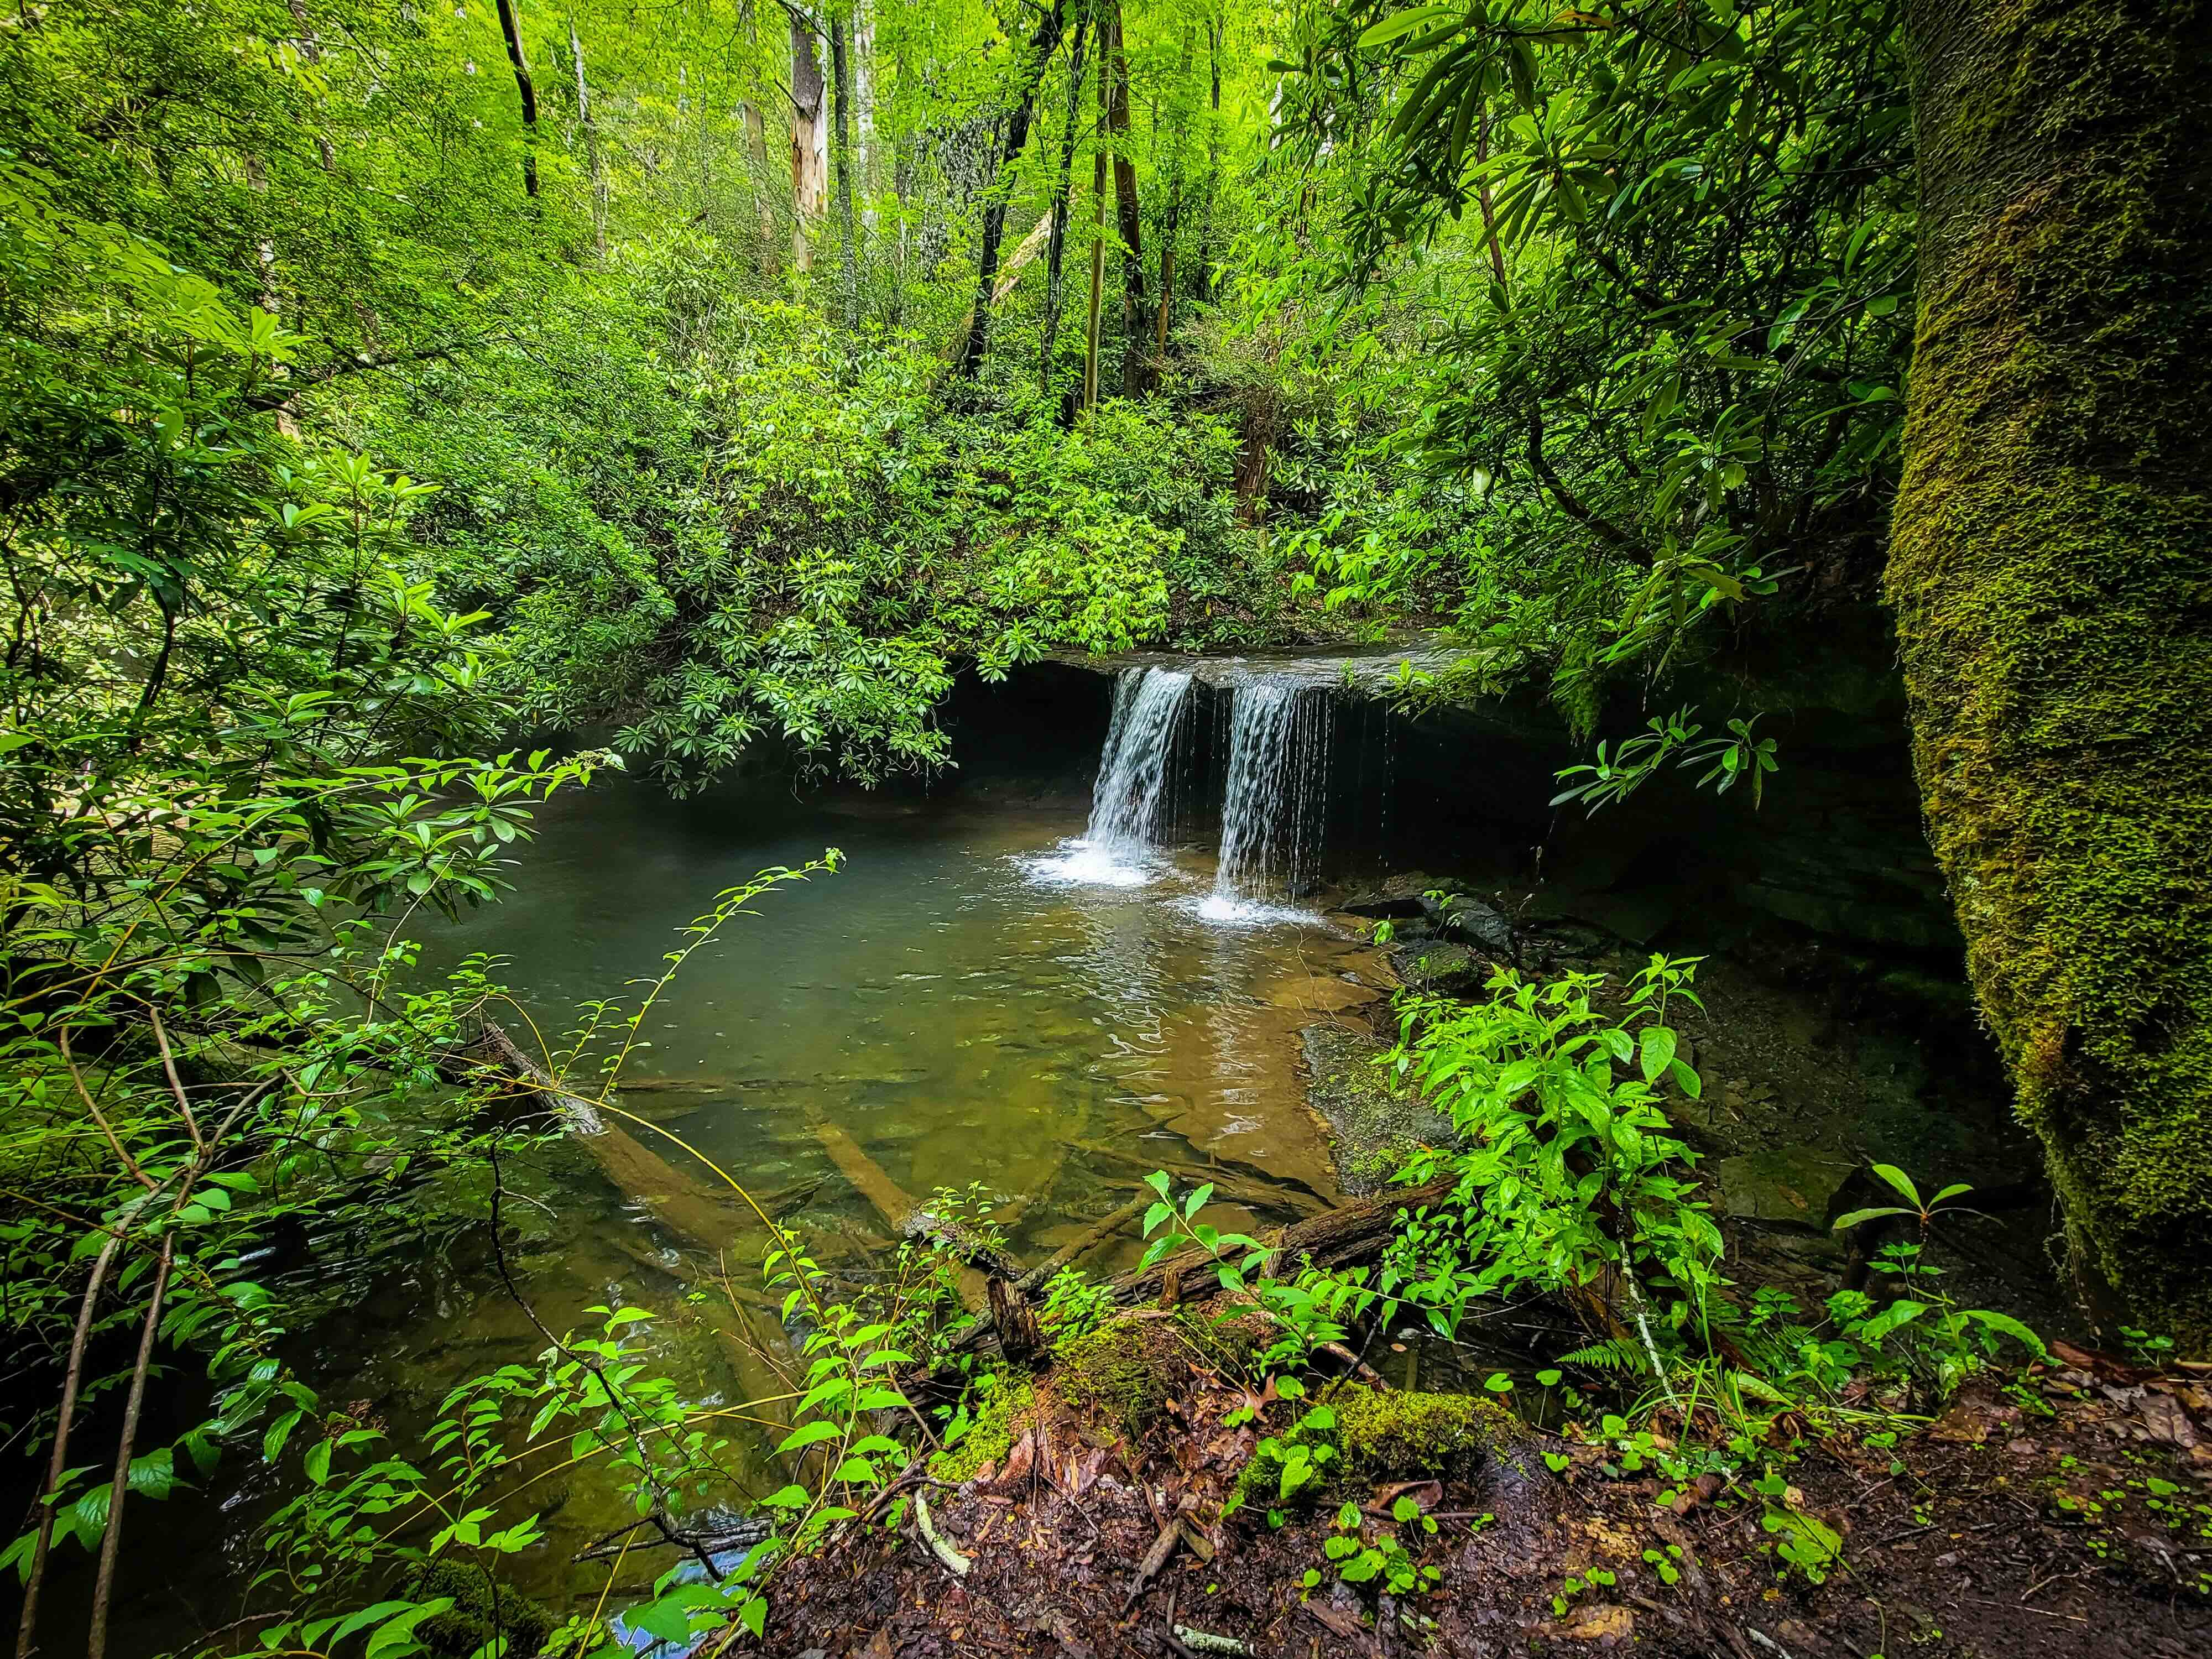
\includegraphics[keepaspectratio]{img/trail-16-figure-01.jpg}}

}

\caption{Photo credit to VioletSkyAdventures}

\end{figure}%

\subsection{Key Characteristics}\label{key-characteristics-16}

\begin{longtable}[]{@{}
  >{\raggedright\arraybackslash}p{(\linewidth - 2\tabcolsep) * \real{0.5400}}
  >{\raggedright\arraybackslash}p{(\linewidth - 2\tabcolsep) * \real{0.4600}}@{}}
\toprule\noalign{}
\begin{minipage}[b]{\linewidth}\raggedright
\textbf{Characteristic}
\end{minipage} & \begin{minipage}[b]{\linewidth}\raggedright
\textbf{Details}
\end{minipage} \\
\midrule\noalign{}
\endhead
\bottomrule\noalign{}
\endlastfoot
Time Estimate & 2.5 hours - 4.5 hours \\
Trail Distance (Miles) & 3.7 \\
Elevation Change & Moderate \\
Pets & Allowed on leash \\
Parking Pass/Entrance Fee & Not Required \\
Restroom(s) & Yes \\
Best Ages & Big kids and Pre-teens and older \\
Strollers and Wheelchairs & Not accessible \\
\end{longtable}

\pandocbounded{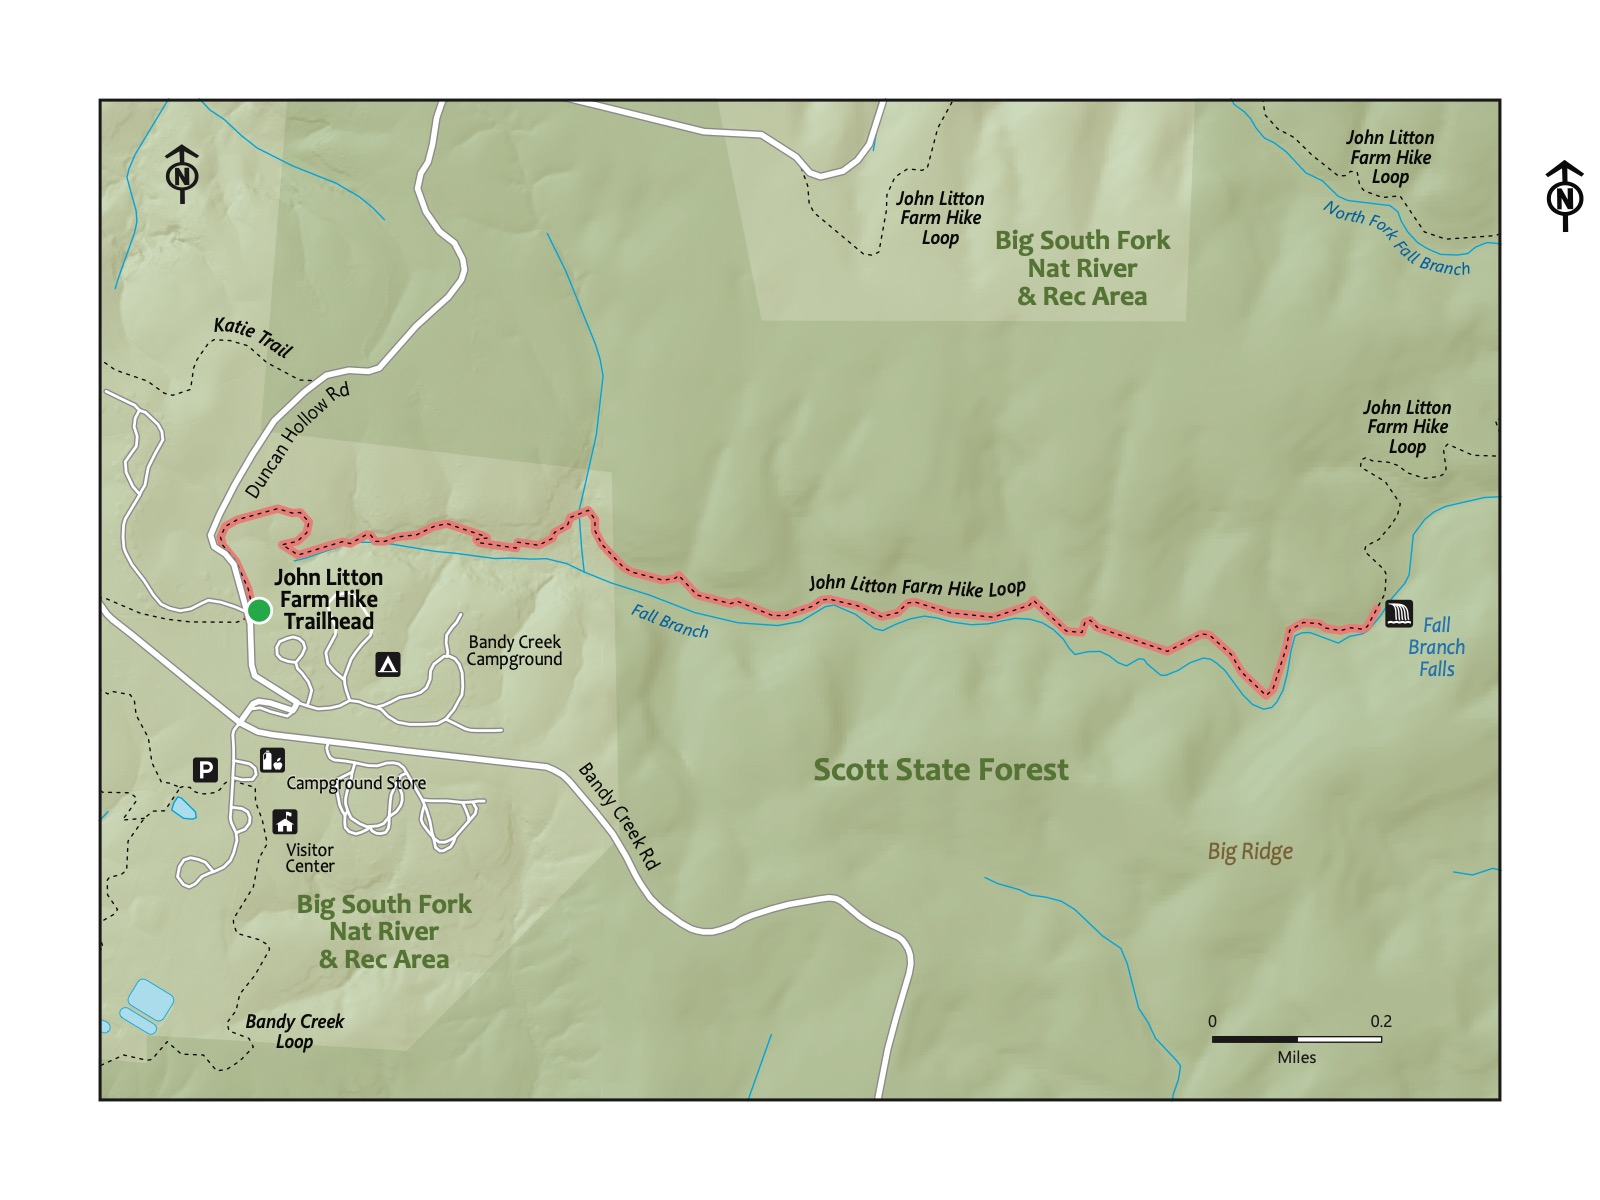
\includegraphics[keepaspectratio]{maps/trail-16-map.jpeg}}

\subsection{Directions to the
Trailhead}\label{directions-to-the-trailhead-15}

Trailhead Address: Bandy Creek Visitors Center, 151 Stable Rd, Oneida,
TN 37841

Trailhead GPS Coordinates: 36.49062, -84.69777

From the Visitors Center, walk across Bandy Loop Road toward the
campground. Find Duncan Hollow Road, and walk up it a short distance,
passing the Bandy Creek Pool, which is another accessible parking area,
on the left. The trailhead is immediately past the pool on the right
side of Duncan Hollow Road.

\subsection{Trail Description}\label{trail-description-15}

\begin{longtable}[]{@{}
  >{\raggedright\arraybackslash}p{(\linewidth - 2\tabcolsep) * \real{0.1875}}
  >{\raggedright\arraybackslash}p{(\linewidth - 2\tabcolsep) * \real{0.8125}}@{}}
\toprule\noalign{}
\begin{minipage}[b]{\linewidth}\raggedright
Distance from Start
\end{minipage} & \begin{minipage}[b]{\linewidth}\raggedright
Description
\end{minipage} \\
\midrule\noalign{}
\endhead
\bottomrule\noalign{}
\endlastfoot
0.0 & Start on the Litten-Slaven Farm Loop Trail. \\
0.2 & Begin to gradually descend into the Fall Branch creekbed. \\
0.5 & Trail levels out. \\
0.55 & Rocky section featuring a short ladder (to make it easier to
navigate through the rocks). \\
1.8 & Fall Branch Falls. A great spot for a break before turning around
to return to the start. \\
3.6 & Trailhead. \\
\end{longtable}

\subsection{Nearby}\label{nearby-15}

\begin{itemize}
\tightlist
\item
  \textbf{Camp at Bandy Creek!} The Bandy Creek Campground is a gem -
  spacious sites, nice restrooms, and lots of cul-de-sacs for kids to
  endlessly play or bike. Consider a stay here as a launching point for
  this hike.
\item
  \textbf{Stop by the visitor's center.} A good place to learn more
  about the Big South Fork and to ask any questions or to seek the
  advice of park rangers.
\item
  \textbf{Hike the nearby Bandy Creek or Angel Falls Trails.} Check out
  the Bandy Creek or Angel Falls Trails chapters. There are hundreds of
  hikes available to you, and any are well worth a hike (the Grand Gap
  Loop is a lengthy favorite!). Consider stopping the the visitor center
  to ask for recommendations and up-to-date information.
\end{itemize}

\chapter{Trail 17: Twin Arches}\label{trail-17-twin-arches}

\subsection{Overview}\label{overview-17}

This short hike leads to one of the most surprising geologic features in
Tennessee! The Twin Arches, a 130-foot span and 100-foot height feature
you can walk over, around, and through. The surrounding forest is not
shabby, either. This is a fantastic and memorable family hike, with some
challenges sprinkled in. First, this hike is the farthest (by driving
distance) of any in this book. Second, there are some rocky sections
that require some carefulness. Still, this is a must-see, and it's near
many features (and places to camp) to make a visit more accommodating.
Good for families with children of any walking age.

\begin{figure}[H]

{\centering \pandocbounded{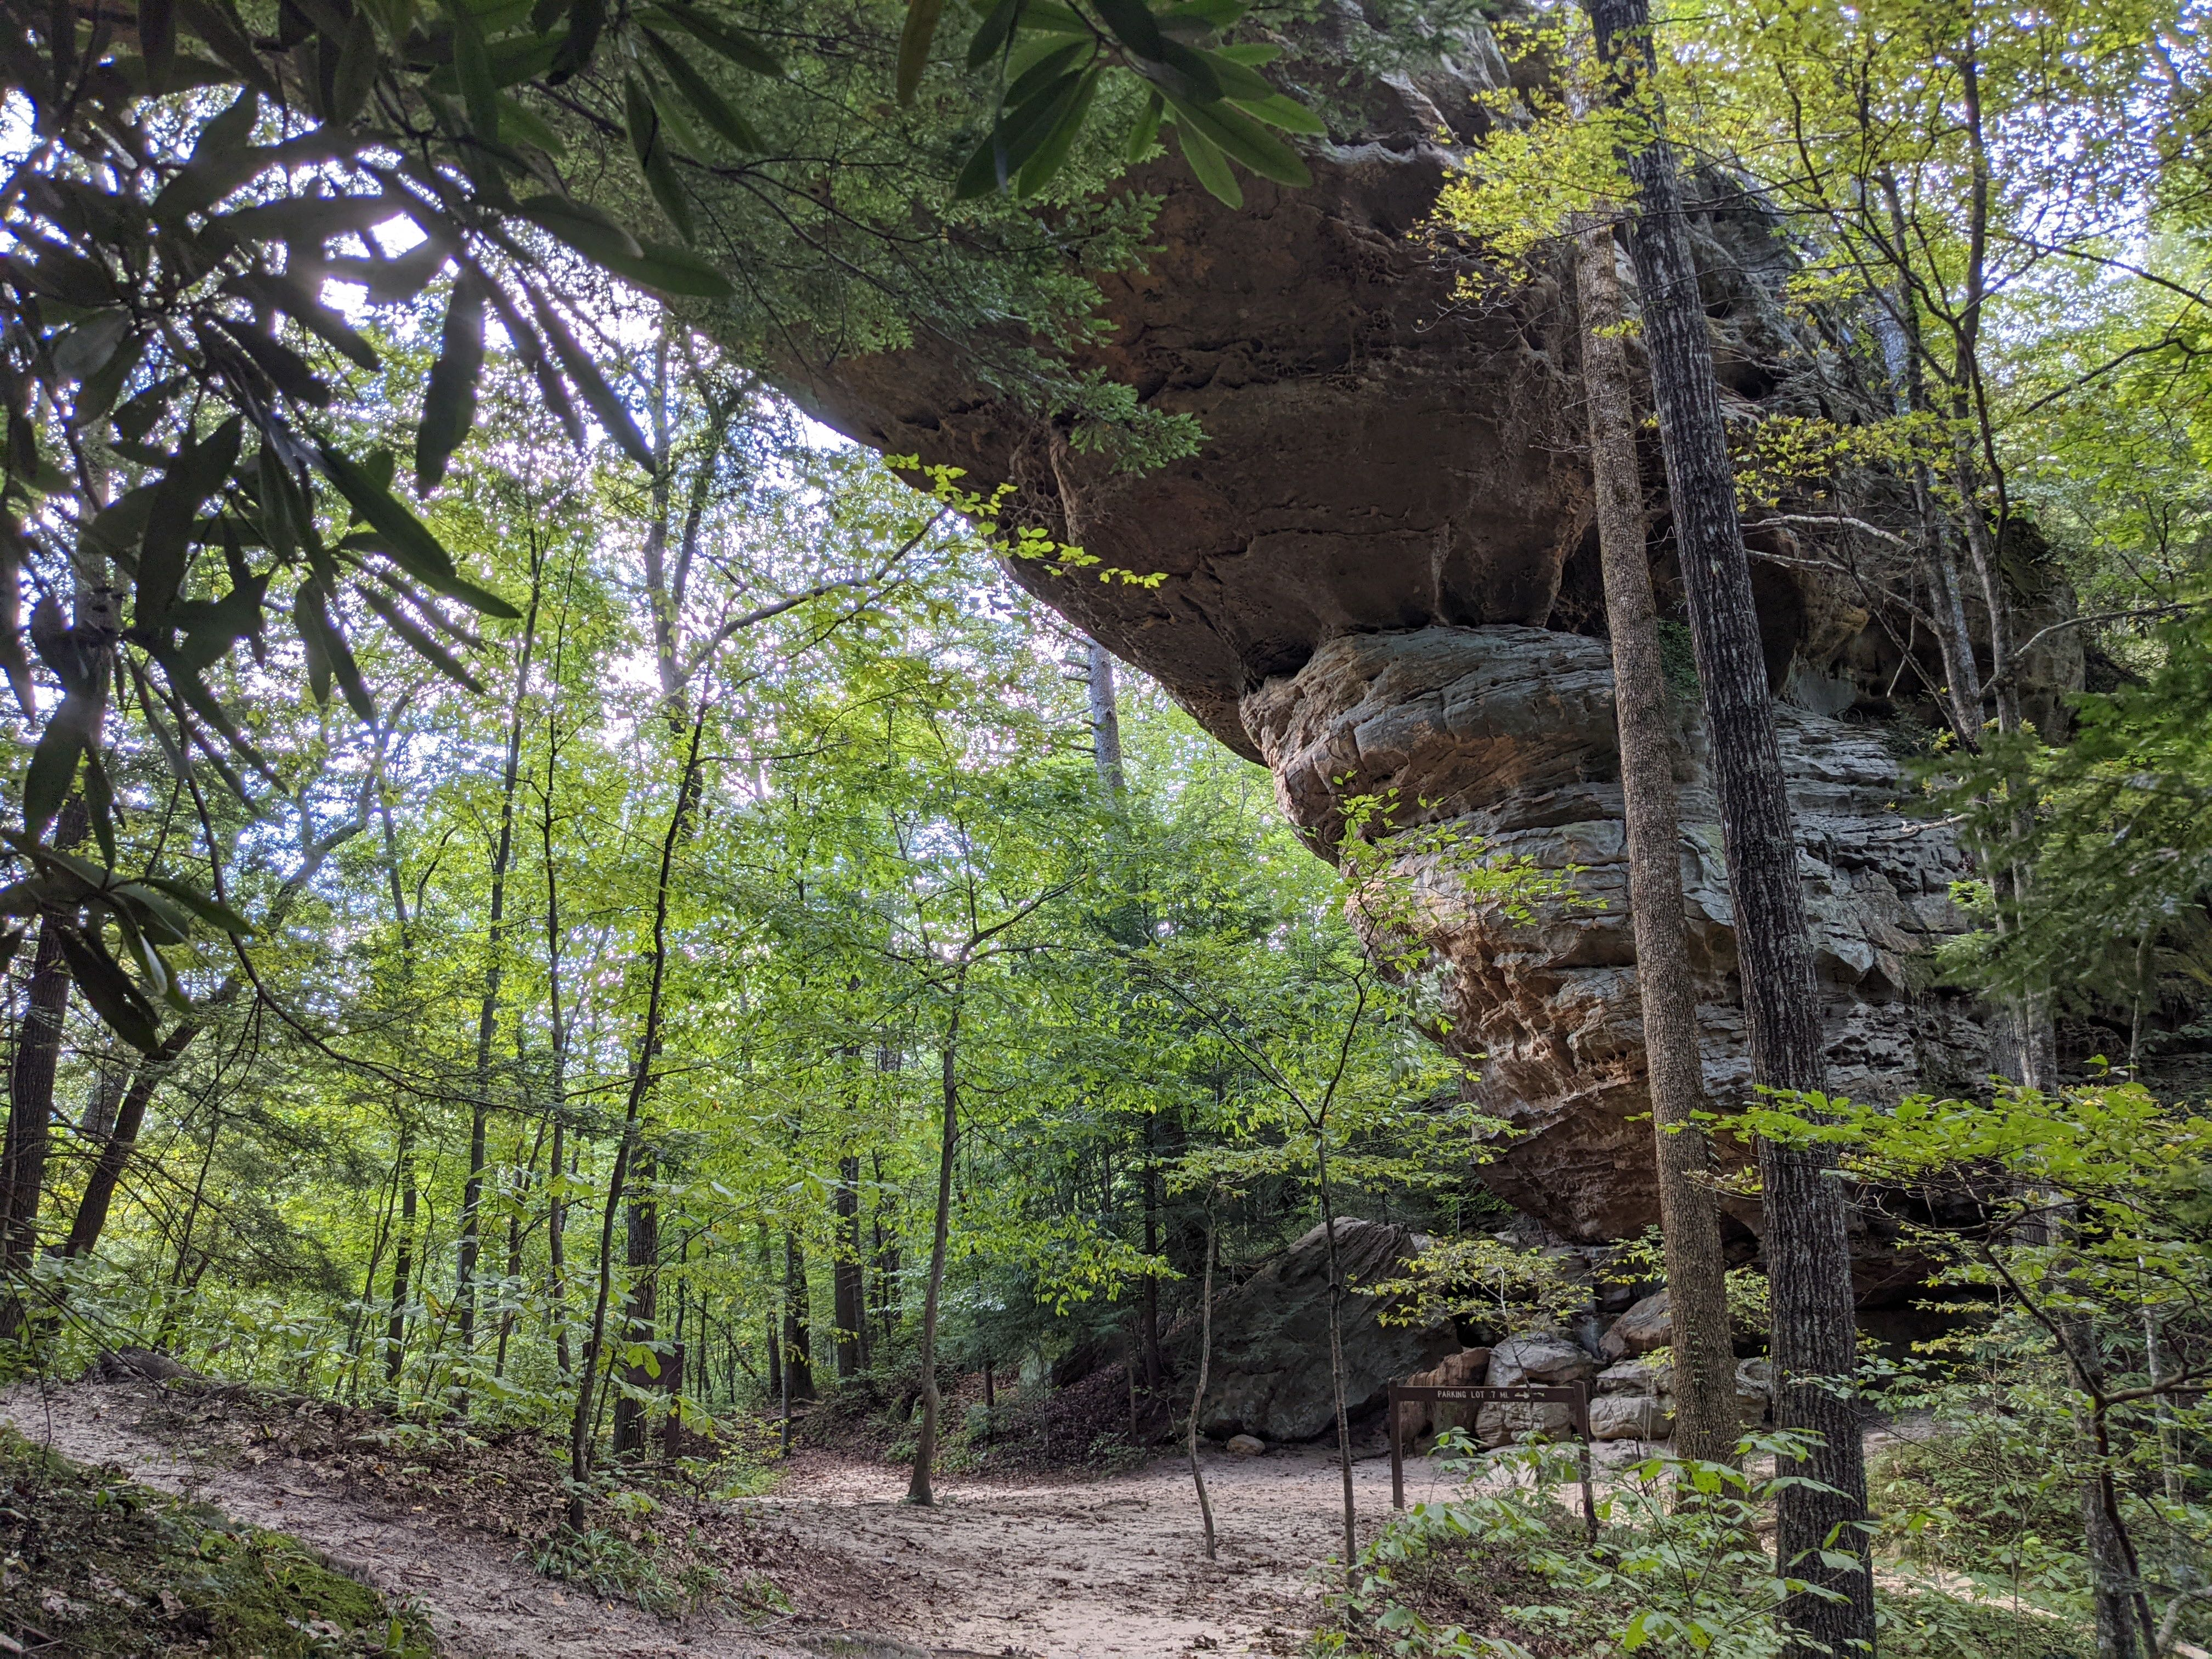
\includegraphics[keepaspectratio]{img/trail-17-figure-01.jpg}}

}

\caption{Photo credit to Katie and Joshua Rosenberg}

\end{figure}%

\subsection{Key Characteristics}\label{key-characteristics-17}

\begin{longtable}[]{@{}
  >{\raggedright\arraybackslash}p{(\linewidth - 2\tabcolsep) * \real{0.5510}}
  >{\raggedright\arraybackslash}p{(\linewidth - 2\tabcolsep) * \real{0.4490}}@{}}
\toprule\noalign{}
\begin{minipage}[b]{\linewidth}\raggedright
\textbf{Characteristic}
\end{minipage} & \begin{minipage}[b]{\linewidth}\raggedright
\textbf{Details}
\end{minipage} \\
\midrule\noalign{}
\endhead
\bottomrule\noalign{}
\endlastfoot
Time Estimate & 1.5 hour - 2.5 hours \\
Trail Distance (Miles) & 1.2 \\
Elevation Change & Moderate \\
Pets & Allowed on leash \\
Parking Pass/Entrance Fee & Not Required \\
Restroom(s) & Yes \\
Best Ages & Little kids and Big kids \\
Strollers and Wheelchairs & Not accessible \\
\end{longtable}

\pandocbounded{\includegraphics[keepaspectratio]{maps/trail-17-map.jpeg}}

\subsection{Directions to the
Trailhead}\label{directions-to-the-trailhead-16}

Trailhead Address: Twin Arches Trailhead, G7V5+Q7 Jamestown, Tennessee

Trailhead GPS Coordinates: 36.48797, -84.69744

\subsection{Trail Description}\label{trail-description-16}

\begin{longtable}[]{@{}
  >{\raggedright\arraybackslash}p{(\linewidth - 2\tabcolsep) * \real{0.1355}}
  >{\raggedright\arraybackslash}p{(\linewidth - 2\tabcolsep) * \real{0.8645}}@{}}
\toprule\noalign{}
\begin{minipage}[b]{\linewidth}\raggedright
Distance from Start
\end{minipage} & \begin{minipage}[b]{\linewidth}\raggedright
Description
\end{minipage} \\
\midrule\noalign{}
\endhead
\bottomrule\noalign{}
\endlastfoot
0.0 & Start on the Twin Arches trail. \\
0.25 & Intersection. Head right to complete the loop in a
counterclockwise section. \\
0.3 & Stairs. \\
0.5 & Arrive at the base of the Twin Arches. Head straight - you won't
be able to miss them! \\
0.6 & Twin Arches. Walk along the top of the arches, under them, and
around them, and then head back toward the loop portion of the trail. \\
0.7 & Turn right at the intersection to complete the loop. \\
0.95 & Intersection. Turn right to return to the trailhead. \\
1.20 & Trailhead. \\
\end{longtable}

\subsection{Nearby}\label{nearby-16}

\begin{itemize}
\tightlist
\item
  \textbf{Camp or rent a cabin at Pickett State Park.} Pickett State
  Park (\%ADDRESS OR WEBSITE\%), a nice campground that also has both
  historic and modern cabins to rent, is close to this trail. It also
  features a great lake for kayaking, canoeing, or paddle boarding.
\item
  \textbf{View the night sky.} Pickett State Park has a Silver-tier
  designation as an International Dark Sky Park. Even if you're not
  strictly in the State Park, this is a great place to view stars and
  planets in the night sky.
\end{itemize}

\chapter{Trail 18: Angel Falls
Overlook}\label{trail-18-angel-falls-overlook}

\subsection{Overview}\label{overview-18}

Like a few of the other trails in or near the Cumberland Plateau, this
is a spectacular hike that is sadly often overlooked. While this
memorable trail is a little tricky to get to for a day hike, the view is
awesome, rivaling the summits of the Smokies, with a different kind of
vantage of the beautiful Big South Fork River. This trail is relatively
flat and short, making it appropriate for families with young children.
Consider camping at the nearby Bandy Creek campground, and consider this
hike a day's excursion from there.

\begin{figure}[H]

{\centering \pandocbounded{\includegraphics[keepaspectratio]{img/trail-18-figure-01.jpg}}

}

\caption{Photo credit to Katie and Joshua Rosenberg}

\end{figure}%

\subsection{Key Characteristics}\label{key-characteristics-18}

\begin{longtable}[]{@{}
  >{\raggedright\arraybackslash}p{(\linewidth - 2\tabcolsep) * \real{0.5400}}
  >{\raggedright\arraybackslash}p{(\linewidth - 2\tabcolsep) * \real{0.4600}}@{}}
\toprule\noalign{}
\begin{minipage}[b]{\linewidth}\raggedright
\textbf{Characteristic}
\end{minipage} & \begin{minipage}[b]{\linewidth}\raggedright
\textbf{Details}
\end{minipage} \\
\midrule\noalign{}
\endhead
\bottomrule\noalign{}
\endlastfoot
Time Estimate & 1.5 hours - 2.5 hours \\
Trail Distance (Miles) & 2.8 \\
Elevation Change & Gentle \\
Pets & Allowed on leash \\
Parking Pass/Entrance Fee & Not Required \\
Restroom(s) & No \\
Best Ages & Little Kids and Big Kids \\
Strollers and Wheelchairs & Not Accessible \\
\end{longtable}

\pandocbounded{\includegraphics[keepaspectratio]{maps/trail-18-map.jpeg}}

\subsection{Directions to the
Trailhead}\label{directions-to-the-trailhead-17}

Trailhead Address: Grand Gap Loop Trailhead, G84V+69 Oneida, Tennessee

Trailhead GPS Coordinates: 36.50549, -84.65664

This address is for the trailhead for the Grand Gap Loop, deep into the
Big South Fork National River \& Recreation Area. The address uses a
Google Maps ``Plus code,'' as there is not a street address for the
trailhead. Please note this only works for Google Maps. Turn right into
the parking area from Alfred Smith Rd. Look for the Grand Gap Loop Trail
to begin the hike.

\begin{tcolorbox}[enhanced jigsaw, colback=white, colframe=quarto-callout-note-color-frame, breakable, opacityback=0, toprule=.15mm, bottomrule=.15mm, rightrule=.15mm, left=2mm, leftrule=.75mm, arc=.35mm]
\begin{minipage}[t]{5.5mm}
\textcolor{quarto-callout-note-color}{\faInfo}
\end{minipage}%
\begin{minipage}[t]{\textwidth - 5.5mm}

\vspace{-3mm}\textbf{Angel Falls}\vspace{3mm}

Angel Falls is more a rapids than a waterfall, but there's a history to
its name: It was a waterfall until the 1940s, when it was dynamited to
make the river more easily navigable by paddlers and boaters. It was
only a little successful: the rapids are known as being impassable for
all but the most intrepid whitewater paddlers.

\end{minipage}%
\end{tcolorbox}

\subsection{Trail Description}\label{trail-description-17}

\begin{longtable}[]{@{}
  >{\raggedright\arraybackslash}p{(\linewidth - 2\tabcolsep) * \real{0.0950}}
  >{\raggedright\arraybackslash}p{(\linewidth - 2\tabcolsep) * \real{0.9050}}@{}}
\toprule\noalign{}
\begin{minipage}[b]{\linewidth}\raggedright
Distance from Start
\end{minipage} & \begin{minipage}[b]{\linewidth}\raggedright
Description
\end{minipage} \\
\midrule\noalign{}
\endhead
\bottomrule\noalign{}
\endlastfoot
0.0 & Start on the Grand Gap Loop (part of the John Muir Trail - these
hikes share a name at this point). Head counterclockwise on the loop
trail; the other direction is a much longer way to the overlook. \\
0.85 & Grave site. \\
1.0 & Descend gently toward the overlook. \\
1.4 & Overlook. Rest and picnic at the large rocky overlook atop the Big
South Fork and Angel Falls. Then, turn around to return to the start. \\
2.8 & Trailhead. \\
\end{longtable}

\begin{figure}[H]

{\centering \pandocbounded{\includegraphics[keepaspectratio]{img/angel-rocks.jpg}}

}

\caption{Photo credit to Katie and Joshua Rosenberg}

\end{figure}%

\subsection{Nearby}\label{nearby-17}

\begin{itemize}
\tightlist
\item
  \textbf{Stop by Bandy Creek.} Check out the Bandy Creek chapter for
  more details.
\item
  \textbf{Hike the Angel Falls Trail}---\textbf{and others.} The Angel
  Falls Trail---not to be mistaken with the trail taken to the overlook
  featured in this hike---starts at the parking area beside the
  Leatherwood Ford Bridge. It follows the Big South Fork River to
  conclude with a close-up view of Angel Falls, but without the vista
  from the overlook. Also, the Big South Fork National River and
  Recreation Area has more than 300 miles of trails.
\end{itemize}

\chapter{Trail 19 : Honey Creek}\label{trail-19-honey-creek}

\subsection{Overview}\label{overview-19}

This hike is unreal! This trail features rope ladders, wooden ladders,
gigantic sandstone walls, a scenic overlook, a trail that traverses
\emph{up} a river, and boulders you crawl over and through. It's
spectacular and challenging. This is a memorable trail that exemplifies
what makes the Cumberland Plateau region such a worthy complement to the
Great Smoky Mountains National Park. Younger children may be able to
hike the first half (traveling counterclockwise from the trailhead); you
can walk the road back to the trailhead. The second half of the trail
contains more challenging (but very beautiful) sections. Still, it's
hard -- probably the most difficult for most in this book, making it
best for the older kiddo hiker. Oh, and you will definitely want to be
prepared to get your feet wet on this hike!

\begin{figure}[H]

{\centering \pandocbounded{\includegraphics[keepaspectratio]{img/trail-19-figure-01.jpg}}

}

\caption{Photo credit to Sam Weisbrod}

\end{figure}%

\subsection{Key Characteristics}\label{key-characteristics-19}

\begin{longtable}[]{@{}
  >{\raggedright\arraybackslash}p{(\linewidth - 2\tabcolsep) * \real{0.5870}}
  >{\raggedright\arraybackslash}p{(\linewidth - 2\tabcolsep) * \real{0.4130}}@{}}
\toprule\noalign{}
\begin{minipage}[b]{\linewidth}\raggedright
\textbf{Characteristic}
\end{minipage} & \begin{minipage}[b]{\linewidth}\raggedright
\textbf{Details}
\end{minipage} \\
\midrule\noalign{}
\endhead
\bottomrule\noalign{}
\endlastfoot
Time Estimate & 4 hours - 7 hours \\
Trail Distance (Miles) & 4.4 \\
Elevation Change & Steep \\
Pets & Not Allowed \\
Parking Pass/Entrance Fee & Required \\
Restroom(s) & No \\
Best Ages & Big kids and Pre-teens and older \\
Strollers and Wheelchairs & Not accessible \\
\end{longtable}

\pandocbounded{\includegraphics[keepaspectratio]{maps/trail-19-map.jpeg}}

\subsection{Directions to the
Trailhead}\label{directions-to-the-trailhead-18}

Trailhead Address: Honey Creek Trailhead and Parking Area, C8CX+G7
Allardt, Tennessee

Trailhead GPS Coordinates: 36.42123, -84.65180

\begin{tcolorbox}[enhanced jigsaw, colback=white, colframe=quarto-callout-note-color-frame, breakable, opacityback=0, toprule=.15mm, bottomrule=.15mm, rightrule=.15mm, left=2mm, leftrule=.75mm, arc=.35mm]
\begin{minipage}[t]{5.5mm}
\textcolor{quarto-callout-note-color}{\faInfo}
\end{minipage}%
\begin{minipage}[t]{\textwidth - 5.5mm}

\vspace{-3mm}\textbf{Rosebay Rhododendron}\vspace{3mm}

These plants are commonly seen on slopes near streams, which helps
stabilize the soil. Looks similar to Mountain Laurel; has larger leaves.
Pretty, but all parts of this plant are toxic to humans and pets!
-MaryRose Weatherton

\end{minipage}%
\end{tcolorbox}

Navigate to the Honey Creek Trailhead. Note that there is also a Honey
Creek Overlook, which is the incorrect start for this hike. The above
address uses a Google Maps ``Plus'' code in lieu of a street address for
this trailhead; it only works in Google Maps.

Park in one of the many spots at the trailhead. The trail begins
slightly past the trailhead, on the other side of the road from the
large signpost for the trailhead, slightly up the road. Look for the
Honey Creek Loop Trail sign.

\subsection{Trail Description}\label{trail-description-18}

\begin{longtable}[]{@{}
  >{\raggedright\arraybackslash}p{(\linewidth - 2\tabcolsep) * \real{0.0950}}
  >{\raggedright\arraybackslash}p{(\linewidth - 2\tabcolsep) * \real{0.9050}}@{}}
\toprule\noalign{}
\begin{minipage}[b]{\linewidth}\raggedright
Distance from Start
\end{minipage} & \begin{minipage}[b]{\linewidth}\raggedright
Description
\end{minipage} \\
\midrule\noalign{}
\endhead
\bottomrule\noalign{}
\endlastfoot
0.0 & Start on the Honey Creek Loop Trail. Gently wind through the
densely wooded forest. \\
0.2 & Gently, then more steeply, descend through the woods. \\
0.9 & Rope ladder. \\
1.05 & Enter the section with high cliff walls along the left of the
trail. \\
1.35 & Trail splits to the left to head to the overlook. Ladders. \\
1.45 & Overlook. After stopping at the overlook, head back down to
resume the trail by turning left at the trail juncture. Or, optionally,
walk the road back 0.8 miles to the parking area and trailhead. \\
1.75 & Trail turns up into Honey Creek. Look for the green symbol with
two hikers as a guide to follow the trail; in places, you'll walk
through the creek and through crevices and cracks in giant boulders! \\
2.25 & Head up and away from the creek. \\
2.75 & Wind through and around huge boulders and rocks. Continue to look
for the green trail symbols. \\
3.0 & Ice Castle Falls, a beautiful waterfall. \\
3.1 & Gentle climb through a rocky, exposed section with different
vegetation. \\
3.25 & Short rope ladder. \\
3.3 & Trail levels out, then climbs back to the start and the
trailhead. \\
4.4 & Trailhead. \\
\end{longtable}

\begin{figure}[H]

{\centering \pandocbounded{\includegraphics[keepaspectratio]{img/jo bsf cliff.jpg}}

}

\caption{Photo credit to Katie and Joshua Rosenberg}

\end{figure}%

\subsection{Nearby}\label{nearby-18}

\begin{itemize}
\tightlist
\item
  \textbf{Grab a slushie!} This is one of the most remote---if not the
  most remote---hikes in this book. A favorite stop on the way back from
  Honey Creek is to quench our thirst by enjoying a slushie at the Pilot
  Travel Center (106 Comfort Ln, Pioneer, TN 37847) off exit 122 on
  I-75.
\end{itemize}

\part{The Great Smoky Mountains National Park}

This section includes informmation on 11 hikes in the Great Smoky
Mountains National Park, or the Smokies. The Smokies are an astonishing
place --- high mountain ridges with plants reminiscent of the northern
United States and even Canada; river and creek beds with abundant
aquatic wildlife; a place of wild bears and stories and the history of
both Cherokee and European settlers still present.

There's no way around these hikes being the heart of this book. That is
not meant to diminish those close to Knoxille and the Cumberland
Plateau, which in other parts of the country would stand apart as
destinations in their own right. It just speaks to how special the
Smokies can be.

That said, a note and a warning. The high number of visitors and the
proximity of Knoxville have key for families: you can be choosy about
when and where to go! While there are few things more special than a
Smokies hike up, for example, a beautiful creek on a perfect Fall day,
there are few things more challenging than being stuck in traffic, no
trail in sight, with tired out kid, or ending up on a trail that feels
more like a line at nearby Dollywood than a hike in the woods. But, this
is the benefit of living in Knoxville, and even in the height of the
summer, there are trails to visit---and times to visit---that will
surprise you with how few people there are!

\pandocbounded{\includegraphics[keepaspectratio]{maps/smokies-region.jpg}}

\chapter{Trail 20: Spruce Flats
Falls}\label{trail-20-spruce-flats-falls}

\subsection{Overview}\label{overview-20}

An adventurous hike in the Smokies accessible to many families, this
hike is also a great introduction to the national park, particularly
when visiting from around Knoxville (it's fairly close). It's on the
Great Smoky Mountains Institute site at Tremont, a national leader in
outdoors and environmental education. It is the first hike in this
section for a good reason. The proximity to Townsend is a bonus. Best
for little kids and big kids. We have hiked this trail with a
two-month-old baby in wrap carrier! Just take your time and watch your
footing. This, at times, challenging hike is well worth it!

\begin{figure}[H]

{\centering \pandocbounded{\includegraphics[keepaspectratio]{img/trail-20-figure-01.jpg}}

}

\caption{Photo credit to Katie and Joshua Rosenberg}

\end{figure}%

\subsection{Key Characteristics}\label{key-characteristics-20}

\begin{longtable}[]{@{}
  >{\raggedright\arraybackslash}p{(\linewidth - 2\tabcolsep) * \real{0.5400}}
  >{\raggedright\arraybackslash}p{(\linewidth - 2\tabcolsep) * \real{0.4600}}@{}}
\toprule\noalign{}
\begin{minipage}[b]{\linewidth}\raggedright
\textbf{Characteristic}
\end{minipage} & \begin{minipage}[b]{\linewidth}\raggedright
\textbf{Details}
\end{minipage} \\
\midrule\noalign{}
\endhead
\bottomrule\noalign{}
\endlastfoot
Time Estimate & 1.5 hours - 2.5 hours \\
Trail Distance (Miles) & 1.6 \\
Elevation Change & Moderate \\
Pets & Not Allowed \\
Parking Pass/Entrance Fee & Required \\
Restroom(s) & Yes \\
Best Ages & Big kids and Pre-teens and older \\
Strollers and Wheelchairs & Not accessible \\
\end{longtable}

\pandocbounded{\includegraphics[keepaspectratio]{maps/trail-20-map.jpeg}}

\subsection{Directions to the
Trailhead}\label{directions-to-the-trailhead-19}

Trailhead Address: 9275 Tremont Rd, Townsend, TN 37882

Trailhead GPS Coordinates: 35.64000, -83.68905

The address and coordinates are for the Great Smoky Mountains Institute,
as this is the easiest-to-locate destination. When nearly there (less
than a quarter of a mile from the destination), you'll cross a bridge to
enter the Institute. You'll see a lot of parking around, as well as a
gift shop. Though the trailhead and Google Maps will navigate you a
little further, the parking you see here is the best place to park. From
this parking lot, walk up the road a little toward the Spruce Flats
Falls Trailhead to start the hike.

\subsection{Trail Description}\label{trail-description-19}

\begin{longtable}[]{@{}
  >{\raggedright\arraybackslash}p{(\linewidth - 2\tabcolsep) * \real{0.1099}}
  >{\raggedright\arraybackslash}p{(\linewidth - 2\tabcolsep) * \real{0.8901}}@{}}
\toprule\noalign{}
\begin{minipage}[b]{\linewidth}\raggedright
Distance from Start
\end{minipage} & \begin{minipage}[b]{\linewidth}\raggedright
Description
\end{minipage} \\
\midrule\noalign{}
\endhead
\bottomrule\noalign{}
\endlastfoot
0.0 & Though the main trail you take to the falls is the Buckeye Trail,
you will start the hike on the Lumber Ridge Trail. Ample signage is
available to help avoid confusion. \\
0.1 & Turn right onto the Buckeye Trail. \\
0.15 & Trail levels out before a steep climb. \\
0.3 & Climb begins. It's a (good) challenge! \\
0.5 & High point of the hike in a piney outcropping. Good photo spot.
Begin to wind down toward the waterfall. \\
0.8 & Spruce Flat Falls. A great snack or picnic spot. After a nice
break, turn around the way you came. \\
1.6 & Trailhead. \\
\end{longtable}

\begin{figure}[H]

{\centering \pandocbounded{\includegraphics[keepaspectratio]{img/spruce-flats-kids.jpg}}

}

\caption{Photo credit to Faith Wood}

\end{figure}%

\subsection{Nearby}\label{nearby-19}

\begin{itemize}
\tightlist
\item
  \textbf{Stop at the Tremont store.} The gift store at Tremont (the
  full name is the Great Smoky Mountains Institute at Tremont) is
  usually open Monday---Friday from 10:00 a.m.---4:00 p.m.
\item
  \textbf{Hike the West Prong trail.} This is a great nearby trail to a
  great picnic spot (at the site of Backcountry Site \#18, across the
  road from the Great Smoky Mountains Institute at Tremont.
\item
  \textbf{Visit Townsend.} See Chestnut Tops trail for more detail.
\end{itemize}

\chapter{Trail 21: Little River}\label{trail-21-little-river}

\subsection{Overview}\label{overview-21}

This hike is a great introduction to the Great Smoky Mountains National
Park by featuring a bit of many of the elements that make the Smokies
special --- a trail along a beautiful, clear river; a waterfall;
abundant plant and aquatic wildlife; deep forest; and human history in
the form of historic cabins. It's close to many amenities, and the drive
from Knoxville is doable in a day. The hike starts at the Little River
trailhead, following the Little River along its namesake river. Turn
around near the small waterfall or continue the loop back to the
trailhead. Great for kids of all ages because there is not any one spot
you must reach on the trail; hike as far as you like and then head back
to the start to picnic or check out the historic cabins!

\begin{figure}[H]

{\centering \pandocbounded{\includegraphics[keepaspectratio]{img/trail-21-figure-01.jpg}}

}

\caption{Photo credit to Katie and Joshua Rosenberg}

\end{figure}%

\subsection{Key Characteristics}\label{key-characteristics-21}

\begin{longtable}[]{@{}
  >{\raggedright\arraybackslash}p{(\linewidth - 2\tabcolsep) * \real{0.5870}}
  >{\raggedright\arraybackslash}p{(\linewidth - 2\tabcolsep) * \real{0.4130}}@{}}
\toprule\noalign{}
\begin{minipage}[b]{\linewidth}\raggedright
\textbf{Characteristic}
\end{minipage} & \begin{minipage}[b]{\linewidth}\raggedright
\textbf{Details}
\end{minipage} \\
\midrule\noalign{}
\endhead
\bottomrule\noalign{}
\endlastfoot
Time Estimate & 3 hours - 5 hours \\
Trail Distance (Miles) & 5.5 \\
Elevation Change & Moderate \\
Pets & Not Allowed \\
Parking Pass/Entrance Fee & Required \\
Restroom(s) & No \\
Best Ages & Little kids, Big kids, and Pre-teens and older \\
Strollers and Wheelchairs & Not accessible \\
\end{longtable}

\pandocbounded{\includegraphics[keepaspectratio]{maps/trail-21-map.jpeg}}

\subsection{Directions to the
Trailhead}\label{directions-to-the-trailhead-20}

Trailhead Address: Elkmont Campground, MC58+3H Gatlinburg, Tennessee
Trailhead GPS Coordinates: 35.65346, -83.58005

Trailhead GPS Coordinates: 35.65346, -83.58005

The trailhead address includes a ``Plus code'' to park at the start of
the Little River Trail --- that parking area does not have a specific
address. If you navigate to ``Elkmont Campground,'' then look for signs
to the parking for the Little River Trail, where this hike begins. Park
and look for the gate across the gravel road, where the Little River
Trail begins.

\begin{tcolorbox}[enhanced jigsaw, colback=white, colframe=quarto-callout-note-color-frame, breakable, opacityback=0, toprule=.15mm, bottomrule=.15mm, rightrule=.15mm, left=2mm, leftrule=.75mm, arc=.35mm]
\begin{minipage}[t]{5.5mm}
\textcolor{quarto-callout-note-color}{\faInfo}
\end{minipage}%
\begin{minipage}[t]{\textwidth - 5.5mm}

\vspace{-3mm}\textbf{Eastern Hemlock}\vspace{3mm}

A tree that ``feels'' like the Smokies - likes shaded groves.
Characterized by its needles being arranged in a flat frond. Threatened
by an invasive species, the Hemlock Wooly Adelgid. While many trees in
the region are affected (look for a white dusty covering of needles),
others are not. Look for it along this trail.

\end{minipage}%
\end{tcolorbox}

\subsection{Trail Description}\label{trail-description-20}

\begin{longtable}[]{@{}
  >{\raggedright\arraybackslash}p{(\linewidth - 2\tabcolsep) * \real{0.2361}}
  >{\raggedright\arraybackslash}p{(\linewidth - 2\tabcolsep) * \real{0.7639}}@{}}
\toprule\noalign{}
\begin{minipage}[b]{\linewidth}\raggedright
Distance from Start
\end{minipage} & \begin{minipage}[b]{\linewidth}\raggedright
Description
\end{minipage} \\
\midrule\noalign{}
\endhead
\bottomrule\noalign{}
\endlastfoot
0.0 & Pass around the gate (it's closed only to vehicles) to begin on
the Little River Trail. \\
0.1 & Pass the Spence Cabin, a histotic cabin that is available to rent
(for the day --- not for nights!). \\
0.45 & Trail begins to ascend. \\
2.1 & Huskey Branch Falls on the right side of the trail. \\
2.4 & Reach the intersection of the Little River Trail and the Cucumber
Gap Trail. Turn right onto the Cucumber Gap trail. Trail climbs up
toward Cucumber Gap. \\
3.4 & Cucumber Gap --- the high point of this hike. Begin to descend. \\
4.65 & Reach the intersection of Cucumber Gap Trail and Jakes Creek
Trail. Turn right onto Jakes Creek Trail. \\
5.3 & Reach Jakes Creek Road. Turn right to return to the trailhead. \\
5.5 & Trailhead. \\
\end{longtable}

\begin{figure}[H]

{\centering \pandocbounded{\includegraphics[keepaspectratio]{img/butterflies.jpg}}

}

\caption{Photo credit to Katie and Joshua Rosenberg}

\end{figure}%

\subsection{Nearby}\label{nearby-20}

\begin{itemize}
\tightlist
\item
  \textbf{Visiting historic cabins.} The nearby historic cabins are a
  must-see. Kids love to duck into and out of many recently restored
  (and others in the process of being restored).
\item
  \textbf{Camping at Elkmont campground.} The Elkmont Campground is
  scenic, large, and worth a visit, especially if you can reserve a spot
  beside the Little River.
\end{itemize}

\chapter{Trail 22: Mouse Creek}\label{trail-22-mouse-creek}

\subsection{Overview}\label{overview-22}

Surprisingly close to Knoxville, given how remote and wild this
trailhead and trail feels, Mouse Creek in the Big Creek area of the
Smokies is quite a bit less well-known than many of the other trails in
the Great Smoky Mountains National Park in this book. The creek that
this trail follows looks otherwordly - clear and almost turquoise in
color. This hike starts at a trailhead at the Big Creek Picnic Area ---
beside the Big Creek Campground. The trail starts off a little steep,
but the trail is wide and smooth; like the Middle Prong trail, this
trail used to be a railroad bed. The trail follows above the creek and
then returns closer to it, with Mouse Creek Falls as the turn-around. A
good day-trip adventure for kids and families; the smooth grade makes
this an achievable hike for younger littles.

\begin{figure}[H]

{\centering \pandocbounded{\includegraphics[keepaspectratio]{img/trail-22-figure-01.jpg}}

}

\caption{Photo credit to Katie and Joshua Rosenberg}

\end{figure}%

\subsection{Key Characteristics}\label{key-characteristics-22}

\begin{longtable}[]{@{}
  >{\raggedright\arraybackslash}p{(\linewidth - 2\tabcolsep) * \real{0.5870}}
  >{\raggedright\arraybackslash}p{(\linewidth - 2\tabcolsep) * \real{0.4130}}@{}}
\toprule\noalign{}
\begin{minipage}[b]{\linewidth}\raggedright
\textbf{Characteristic}
\end{minipage} & \begin{minipage}[b]{\linewidth}\raggedright
\textbf{Details}
\end{minipage} \\
\midrule\noalign{}
\endhead
\bottomrule\noalign{}
\endlastfoot
Time Estimate & 2 hours - 4 hours \\
Trail Distance (Miles) & 4.0 \\
Elevation Change & Moderate \\
Pets & Not Allowed \\
Parking Pass/Entrance Fee & Required \\
Restroom(s) & Yes (seasonal) \\
Best Ages & Little kids and Big kids \\
Strollers and Wheelchairs & Not accessible \\
\end{longtable}

\pandocbounded{\includegraphics[keepaspectratio]{maps/trail-22-map.jpeg}}

\subsection{Directions to the
Trailhead}\label{directions-to-the-trailhead-21}

Trailhead Address: Big Creek Picnic Area, QV2R+H6 Newport, Tennessee
Trailhead GPS Coordinates: 35.75132, -83.10964

Trailhead GPS Coordinates: 35.75132, -83.10964

Navigate to the Big Creek Picnic Area. Note that the above address uses
a Google Maps ``Plus code'' in the absence of a street address for this
picnic area; the plus code only works in Google Maps. The picnic area is
at the end of a bumpy dirt road; it's large and easy to find. You may
note the Big Creek Trailhead on the way (it was on the right,
immediately before the parking lot). Park and then backtrack a little on
the road you took to the parking area to find the start of this trail.
Kids may like to play around the picnic area (and the pretty bridge
crossing Big Creek) before or after the hike!

\begin{tcolorbox}[enhanced jigsaw, colback=white, colframe=quarto-callout-note-color-frame, breakable, opacityback=0, toprule=.15mm, bottomrule=.15mm, rightrule=.15mm, left=2mm, leftrule=.75mm, arc=.35mm]
\begin{minipage}[t]{5.5mm}
\textcolor{quarto-callout-note-color}{\faInfo}
\end{minipage}%
\begin{minipage}[t]{\textwidth - 5.5mm}

\vspace{-3mm}\textbf{Blue Ridge Two-Lined Salamander}\vspace{3mm}

The Great Smoky Mountains has more than 30 species of salamanders -- one
of the types of species that contributes to and characterizes the
incredible biodiversity of the Smokies. The Blue Ridge Two-Lined
Salamander is among the most beautiful salamanders, with its
yellow-to-orange coloring and stark black stripes.\\
- Amanda Garner

\end{minipage}%
\end{tcolorbox}

\subsection{Trail Description}\label{trail-description-21}

\begin{longtable}[]{@{}
  >{\raggedright\arraybackslash}p{(\linewidth - 2\tabcolsep) * \real{0.2639}}
  >{\raggedright\arraybackslash}p{(\linewidth - 2\tabcolsep) * \real{0.7361}}@{}}
\toprule\noalign{}
\begin{minipage}[b]{\linewidth}\raggedright
Distance from Start
\end{minipage} & \begin{minipage}[b]{\linewidth}\raggedright
Description
\end{minipage} \\
\midrule\noalign{}
\endhead
\bottomrule\noalign{}
\endlastfoot
0.0 & Start on the Big Creek Trail. Gradually ascend. \\
0.1 & Ascend grardually on a wide path. \\
1.4 & Midnight Hole Falls. Great swimming spot in the summer. \\
2.0 & Mouse Creek Falls. Turn-around spot. Head back to the start.
Optionally, continue farther on the trail. \\
4.0 & Trailhead. \\
\end{longtable}

\begin{figure}[H]

{\centering \pandocbounded{\includegraphics[keepaspectratio]{img/trail-22-figure-02.jpg}}

}

\caption{Photo credit to Dean Pennala}

\end{figure}%

\subsection{Nearby}\label{nearby-21}

\begin{itemize}
\tightlist
\item
  \textbf{Picnicking at a lovely picnic area.} The Big Creek Picnic Area
  is one of the finest spots to picnic in the Great Smoky Mountains
  National Park. Start or end your hike with a picnic here.
\end{itemize}

\chapter{Trail 23: Whiteoak Sink}\label{trail-23-whiteoak-sink}

\subsection{Overview}\label{overview-23}

This is the wildflower hike in the Smokies. It's a joy in mid-late
April, depending on the year's weather. This hike starts on the
kid-friendly Schoolhouse Gap trail and then connects to the Whiteoak
Sink trail, which is a bit rockier but still hike-able by younger
children. You may notice that Whiteoak Sink does not appear on the
National Park Service trail map for the Smokies; technically, Whiteoak
Sink is not an official trail in the Great Smoky Mountains National
Park, and the key takeaway for hikers is to respect this unique area of
the park by staying on the trail and refraining to pick wildflowers. It
is a must-hike during wildflower season, but also worth a trip outside
of that elusive spring period. Because of the length, best for younger
kids who are carried some or all of the way, or kids who are comfortable
with a longer hike.

\begin{figure}[H]

{\centering \pandocbounded{\includegraphics[keepaspectratio]{img/trail-23-figure-01.jpg}}

}

\caption{Photo credit to Katie and Joshua Rosenberg}

\end{figure}%

\subsection{Key Characteristics}\label{key-characteristics-23}

\begin{longtable}[]{@{}
  >{\raggedright\arraybackslash}p{(\linewidth - 2\tabcolsep) * \real{0.5870}}
  >{\raggedright\arraybackslash}p{(\linewidth - 2\tabcolsep) * \real{0.4130}}@{}}
\toprule\noalign{}
\begin{minipage}[b]{\linewidth}\raggedright
\textbf{Characteristic}
\end{minipage} & \begin{minipage}[b]{\linewidth}\raggedright
\textbf{Details}
\end{minipage} \\
\midrule\noalign{}
\endhead
\bottomrule\noalign{}
\endlastfoot
Time Estimate & 3 hours - 5 hours \\
Trail Distance (Miles) & 4.6 \\
Elevation Change & Moderate \\
Pets & Not Allowed \\
Parking Pass/Entrance Fee & Required \\
Restroom(s) & No \\
Best Ages & Little kids and Big kids \\
Strollers and Wheelchairs & Not accessible \\
\end{longtable}

\pandocbounded{\includegraphics[keepaspectratio]{maps/trail-23-map.jpeg}}

\subsection{Directions to the
Trailhead}\label{directions-to-the-trailhead-22}

Trailhead Address: Schoolhouse Gap Trailhead, J7GF+W9, Townsend, TN
37882

Trailhead GPS Coordinates: 35.62718, -83.72650

The above address is for the parking area beside the trail. Please note
it uses a Google Maps ``Plus code'', as this trailhead does not have a
street address. This plus code only works in Google Maps. Park, and look
for several large boulders next to a sign for the Schoolhouse Gap Trail
to begin the hike.

\begin{tcolorbox}[enhanced jigsaw, colback=white, colframe=quarto-callout-note-color-frame, breakable, opacityback=0, toprule=.15mm, bottomrule=.15mm, rightrule=.15mm, left=2mm, leftrule=.75mm, arc=.35mm]
\begin{minipage}[t]{5.5mm}
\textcolor{quarto-callout-note-color}{\faInfo}
\end{minipage}%
\begin{minipage}[t]{\textwidth - 5.5mm}

\vspace{-3mm}\textbf{Trillium}\vspace{3mm}

Native perennial plants with distinctive three-petal flowers that bloom
in the spring. These shade-loving plants are often found in the forest
understory, where their seeds are dispersed and buried by ants, in a
process called myrmecochory. Trillium plants are protected in many
places because they are extremely slow-growing. For some species, it can
take anywhere from 5-9 years from being planted to their first bloom; a
single plant can live up to 25 years! So, next time you see one, make
sure you appreciate their beauty with your eyes only.\\
- MaryRose Weatherton

\end{minipage}%
\end{tcolorbox}

\subsection{Trail Description}\label{trail-description-22}

\begin{longtable}[]{@{}
  >{\raggedright\arraybackslash}p{(\linewidth - 2\tabcolsep) * \real{0.2222}}
  >{\raggedright\arraybackslash}p{(\linewidth - 2\tabcolsep) * \real{0.7778}}@{}}
\toprule\noalign{}
\begin{minipage}[b]{\linewidth}\raggedright
Distance from Start
\end{minipage} & \begin{minipage}[b]{\linewidth}\raggedright
Description
\end{minipage} \\
\midrule\noalign{}
\endhead
\bottomrule\noalign{}
\endlastfoot
0.0 & Start on the Schoolhouse Gap Trail. Trail very gradually
ascends. \\
0.4 & Trail climbs more steeply (but managably!). \\
1.1 & Intersection with the trail to Whiteoak Sink. Note that Whiteoak
Sink is not an official trail on the official trail map for the Great
Smoky Mountains National Park; thus, the trail is not as well marked as
most others. Turn left from the Schoolhouse Gap trail onto the trail to
Whiteoak Sink. Descend for around .25 miles. \\
1.4 & Ascend steeply through a pretty and densely wooded forest. \\
1.7 & High point. Descend into Whiteoak Sink. \\
1.9 & Reach an intersection. The trail to the right heads to Rainbow
Cave Falls (different from and not to be confused with the Rainbow Falls
Trail near Gatlinburg!). After stopping at the waterfall, turn around to
return to the intersection of the primary trail. \\
2.2 & Turn right back onto the primary trail. Enter the part of the
trail with the densest understory of wildflowers. Tread carefully; stay
on the trail to not damage any of the plants near to the trail. \\
2.35 & Reach the large bat cave ahead of the end of the trail. Still
tread carefully (and do not attempt to enter the caves for your safety
and to not endanger the bats). Optionally, turn right or left to explore
more of this special area. Then, turn around to return along the trail
you took into Whiteoak Sink. Return to the start. \\
4.6 & Trailhead. \\
\end{longtable}

\begin{figure}[H]

{\centering \pandocbounded{\includegraphics[keepaspectratio]{img/sign for whiteoak.jpeg}}

}

\caption{Photo credit to Katie and Joshua Rosenberg}

\end{figure}%

\subsection{Nearby}\label{nearby-22}

\begin{itemize}
\tightlist
\item
  ****Exploring the Cades Cove loop.**** A drive around the Cades Cove
  Loop can complement a hike to Whiteoak Sink. We recommend only driving
  this beautiful loop road outside of the busiest times (summer and fall
  weekends and holidays, mainly) when traffic can be intense. Consult
  the Abrams Fall hike for additional details on this area and nearby
  amenities.
\item
  ****Visiting Townsend.**** Like the Chestnut Tops hike, visiting ``The
  Peaceful Side of the Smokies,'' Townsend, is a great way to end this
  trip to the Great Smoky Mountains National Park.
\item
  ****Hiking the West Prong Trail.**** The nearby West Prong Trail is a
  favorite that didn't quite make it into this book, but it is still a
  worthy destination. Instead of hiking up Schoolhouse Gap (like for
  this trail), cross the road and hike to the scenic backpacking site
  \#18 as the turn-around spot beside a wood log bridge and pretty
  creek.
\end{itemize}

\chapter{Trail 24: Middle Prong}\label{trail-24-middle-prong}

\subsection{Overview}\label{overview-24}

This hike is great for families looking to have an authentic hiking
experience deep in the Smokies while still being only a little over an
hour's drive from Knoxville. A benefit of this hike is its
distance--only 0.6 miles to the waterfall, but along a stream that
affords many chances to hop in and splash. The turn-around spot is an
overlook to a waterfall, Lynn Camp Prong, though the trail continues
after the cascades up to another waterfall, Indian Flats Falls. Given
the ample shade and easy access to the stream, this is a great hike for
the summer, but it is enjoyable in all seasons. Good for kids of all
ages because you can turn around at any point.

\begin{figure}[H]

{\centering \pandocbounded{\includegraphics[keepaspectratio]{img/trail-24-figure-01.jpg}}

}

\caption{Photo credit to Katie and Joshua Rosenberg}

\end{figure}%

\subsection{Key Characteristics}\label{key-characteristics-24}

\begin{longtable}[]{@{}ll@{}}
\toprule\noalign{}
\textbf{Characteristic} & \textbf{Details} \\
\midrule\noalign{}
\endhead
\bottomrule\noalign{}
\endlastfoot
Time Estimate & 4 hours - 6 hours \\
Trail Distance (Miles) & 7.6 \\
Elevation Change & Moderate \\
Pets & Not Allowed \\
Parking Pass/Entrance Fee & Required \\
Restroom(s) & No \\
Best Ages & All Ages \\
Strollers and Wheelchairs & Not accessible \\
\end{longtable}

\pandocbounded{\includegraphics[keepaspectratio]{maps/trail-24-map.jpeg}}

\subsection{Directions to the
Trailhead}\label{directions-to-the-trailhead-23}

Trailhead Address: Middle Prong Trail Trailhead, J89J+54 Townsend,
Tennessee

Trailhead GPS Coordinates: 35.61794, -83.66971

The above address will navigate you to the parking area for the
trailhead. Please note it uses a ``Plus code'' in lieu of a stree
address that only works in Google Maps. Note that this trailhead is at
the end of a lengthy gravel road, but it's fairly smooth (and it's a
pretty drive). This is a large parking area. Even on the busiest days,
you will be able to find a place to park. There are spots around the
turn-around, but, if they are taken, it is acceptable to park on the
side of the road. After parking, walk toward the bridge to start your
hike.

\begin{tcolorbox}[enhanced jigsaw, colback=white, colframe=quarto-callout-note-color-frame, breakable, opacityback=0, toprule=.15mm, bottomrule=.15mm, rightrule=.15mm, left=2mm, leftrule=.75mm, arc=.35mm]
\begin{minipage}[t]{5.5mm}
\textcolor{quarto-callout-note-color}{\faInfo}
\end{minipage}%
\begin{minipage}[t]{\textwidth - 5.5mm}

\vspace{-3mm}\textbf{Brook Trout}\vspace{3mm}

The native species of trout in Smokies streams. Speckled and small.
Found at high elevations, whereas the Rainbow Trout and Brown Trout were
later introduced for fishing.

\end{minipage}%
\end{tcolorbox}

\subsection{Trail Description}\label{trail-description-23}

\begin{longtable}[]{@{}
  >{\raggedright\arraybackslash}p{(\linewidth - 2\tabcolsep) * \real{0.2639}}
  >{\raggedright\arraybackslash}p{(\linewidth - 2\tabcolsep) * \real{0.7361}}@{}}
\toprule\noalign{}
\begin{minipage}[b]{\linewidth}\raggedright
Distance from Start
\end{minipage} & \begin{minipage}[b]{\linewidth}\raggedright
Description
\end{minipage} \\
\midrule\noalign{}
\endhead
\bottomrule\noalign{}
\endlastfoot
0.0 & Cross the bridge over Lynn Camp Prong. Ascend gradually on the
Middle Prong Trail. \\
0.05 & Almost immediately past the bridge, not the split in the trail.
This hike heads to the left. A short trail, the Thunderhead Prong Quiet
Walkway, heads to the left (it's a great place for kids to play and
splash on hot days!). \\
0.65 & Overlook to Lynn Camp Prong. Though a short way in, this is an
acceptable spot to turn around and head back to the start. The trail
continues onward. This is one of many trails in the Smokies that is
pretty and very worthwhile all along the way; hike as far as you or your
littles like. \\
2.35 & Intersection with Panther Creek Trail on the left. Continue on
the Middle Prong Trail. \\
3.6 & Begin a brief switchback before the waterfall at the end of this
hike. \\
3.8 & Reach Indian Flat Falls. Look for a little opening in the trees
and shrubs. You'll find it! After resting at the beautiful waterfall,
turn around to return to the start. \\
5.25 & Intersection with the Panther Creek Trail on the right. \\
7.6 & Trailhead \\
\end{longtable}

\begin{figure}[H]

{\centering \pandocbounded{\includegraphics[keepaspectratio]{img/jo middle prong.jpg}}

}

\caption{Photo credit to Katie and Joshua Rosenberg}

\end{figure}%

\subsection{Nearby}\label{nearby-23}

\begin{itemize}
\tightlist
\item
  Driving the Cade's Cove Loop. This is a nice way to make a longer day
  of your trip. Instead of returning the way you came, at the
  intersection of Townsend Road and Laurel Creek Road, turn left and
  head toward Cade's Cove. The drive to Cade's Cove is around 15
  minutes; the loop road around Cade's Cove takes around 45 minutes to
  drive--longer on busy days, especially when bears are visible--which
  is often! Traffic on the loop road can be severe, especially during
  peak times, so plan accordingly to avoid restless kiddos.
\item
  \textbf{Stopping for a snack or meal in Townsend.} Townsend bills
  itself as the ``Peaceful Side of the Smokies''. Peaceful Side Social
  is a favorite lunch and dinner spot with kids, owing to the good food
  and large outdoor play area.
\end{itemize}

\chapter{Trail 25: Abrams Creek}\label{trail-25-abrams-creek}

\subsection{Overview}\label{overview-25}

Abrams Creek is a great place to start hiking in the Smokies if you live
in or around Knoxville. It's accessible, offers a wide variety of
features to please all members of the family, and has the added bonus of
being beautiful! The enduring memory from this trail is of kids
splashing endlessly in the shallow creeks. This was the first place we
traveled as a family in the Smokies, and we returned again and again
because we always enjoyed our time together there. There are many ways
to shorten the hike, and we often hike around a mile in and then turn
around. It can be warmer here in the summer months, but the river offers
many opportunities to swim and splash around, making it a great
destination for the summer as well. This hike is relatively challenging
and better suited to hiking in its entirety with older children, but the
beauty of this hike is its versatility: you can turn-around at many
points along the trail and still have a great hike!

\begin{figure}[H]

{\centering \pandocbounded{\includegraphics[keepaspectratio]{img/trail-25-figure-01.jpg}}

}

\caption{Photo credit to Sam Weisbrod}

\end{figure}%

\subsection{Key Characteristics}\label{key-characteristics-25}

\begin{longtable}[]{@{}ll@{}}
\toprule\noalign{}
\textbf{Characteristic} & \textbf{Details} \\
\midrule\noalign{}
\endhead
\bottomrule\noalign{}
\endlastfoot
Time Estimate & 4 hours - 6 hours \\
Trail Distance (Miles) & 5.8 \\
Elevation Change & Moderate \\
Pets & Not Allowed \\
Parking Pass/Entrance Fee & Required \\
Restroom(s) & Yes (seasonal) \\
Best Ages & All ages \\
Strollers and Wheelchairs & Not accessible \\
\end{longtable}

\pandocbounded{\includegraphics[keepaspectratio]{maps/trail-25-map.jpeg}}

\subsection{Directions to the
Trailhead}\label{directions-to-the-trailhead-24}

Trailhead Address: Abrams Creek Campground, J368+MR Tallassee, Tennessee

Trailhead GPS Coordinates: 35.61095, -83.93356

\begin{tcolorbox}[enhanced jigsaw, colback=white, colframe=quarto-callout-note-color-frame, breakable, opacityback=0, toprule=.15mm, bottomrule=.15mm, rightrule=.15mm, left=2mm, leftrule=.75mm, arc=.35mm]
\begin{minipage}[t]{5.5mm}
\textcolor{quarto-callout-note-color}{\faInfo}
\end{minipage}%
\begin{minipage}[t]{\textwidth - 5.5mm}

\vspace{-3mm}\textbf{The Cherokee}\vspace{3mm}

The people of the Cherokee Nation were indigenous to a vast area to the
south, east, and west of the Smokies; the Smokies were more a place for
gathering and hunting than residing. The Eastern Band of the Cherokee
remains an autonomous Nation just south of the Smokies.

\end{minipage}%
\end{tcolorbox}

It never seems to become crowded at Abrams Creek, but parking can be a
bit confusing. This is because the campground is further along the same
road the trailhead is on. Also, there are two areas to park for the
trailhead. We usually park by the gate to the campground, but you can
also park near the large sign with maps of this area of the national
park.

\subsection{Trail Description}\label{trail-description-24}

\begin{longtable}[]{@{}
  >{\raggedright\arraybackslash}p{(\linewidth - 2\tabcolsep) * \real{0.2361}}
  >{\raggedright\arraybackslash}p{(\linewidth - 2\tabcolsep) * \real{0.7639}}@{}}
\toprule\noalign{}
\begin{minipage}[b]{\linewidth}\raggedright
Distance from Start
\end{minipage} & \begin{minipage}[b]{\linewidth}\raggedright
Description
\end{minipage} \\
\midrule\noalign{}
\endhead
\bottomrule\noalign{}
\endlastfoot
0.0 & Start at the trailhead parking area. Walk along the road beside
Abrams Creek. \\
0.4 & Arrive at the campground. A great spot to rest and hang out by the
creek. \\
1.0 & Cross Kingfisher Creek for the first time. Watch for rocks and
branches to aid in crossing. \\
1.1 & Cross Kingfisher Creek again about 100 yards past the first
crossing. \\
1.3 & Reach Backcountry Site \#1. Frequently used by overnight
backpackers; a good resting spot. We often turn around here! \\
1.5 & Reach the top of the ridge after a steep climb. Another great
place to stop and rest (or turn around). Or continue for a grand
adventure. \\
1.6 & Arrive at the overlook with views of Abrams Creek and Gregory Bald
in the distance. \\
2.0 & Return to Abrams Creek near its intersection with Buckshank
Branch. A great spot to relax and splash in the creek. \\
2.8 & Reach Backcountry Site \#17. Turn around here to head back to the
start. \\
4.3 & Return to Backcountry Site \#1. \\
5.6 & Trailhead. \\
\end{longtable}

\begin{figure}[H]

{\centering \pandocbounded{\includegraphics[keepaspectratio]{img/trail-25-figure-02.jpg}}

}

\caption{Photo credit to Katie and Joshua Rosenberg}

\end{figure}%

\subsection{Nearby}\label{nearby-24}

\begin{itemize}
\tightlist
\item
  \textbf{Visiting the Look Rock Overlook.} Check the Look Rock Overlook
  hike for a short, nearby hike to a pretty overlook.
\item
  \textbf{Camping at Abrams Creek Campground.} This is a lovely
  creekside campground that you pass on this hike. Consider a stay in
  the summer, when jumping in the cool, not-too-deep creek can be a
  respite from the heat---or in the fall when this area pops with fall
  colors.
\end{itemize}

\chapter{Trail 26: Look Rock}\label{trail-26-look-rock}

\subsection{Overview}\label{overview-26}

This is a short but rewarding overlook hike that is just a moderate
drive from Knoxville. The entire hike is paved --- but the trail is
steep. Start at a parking area with a very scenic overlook. The trail
starts steep but then levels out. At the top is a tower that affords
views of the Smokies as well as the Tennessee Valley and Knoxville.
Clear days are more often found in the winter, spring, and fall (after
the humidity drops). Consider coupling with a drive along the Foothills
Parkway, or take visitors here after you pick them up from the airport
in nearby Maryville, as we have with our parents! This is a fun family
thike with littles that serve as a nice and usually not crowded
introduction to the Smokies.

\begin{figure}[H]

{\centering \pandocbounded{\includegraphics[keepaspectratio]{img/trail-26-figure-01.jpg}}

}

\caption{Photo credit to Katie and Joshua Rosenberg}

\end{figure}%

\subsection{Key Characteristics}\label{key-characteristics-26}

\begin{longtable}[]{@{}
  >{\raggedright\arraybackslash}p{(\linewidth - 2\tabcolsep) * \real{0.5625}}
  >{\raggedright\arraybackslash}p{(\linewidth - 2\tabcolsep) * \real{0.4375}}@{}}
\toprule\noalign{}
\begin{minipage}[b]{\linewidth}\raggedright
\textbf{Characteristic}
\end{minipage} & \begin{minipage}[b]{\linewidth}\raggedright
\textbf{Details}
\end{minipage} \\
\midrule\noalign{}
\endhead
\bottomrule\noalign{}
\endlastfoot
Time Estimate & 30 minutes - 1 hour \\
Trail Distance (Miles) & 0.6 \\
Elevation Change & Moderate \\
Pets & Not Allowed \\
Parking Pass/Entrance Fee & Required \\
Restroom(s) & No \\
Best Ages & Toddlers and Little Kids \\
Strollers and Wheelchairs & Partially accessible (paved but very
steep) \\
\end{longtable}

\pandocbounded{\includegraphics[keepaspectratio]{maps/trail-26-map.jpeg}}

\subsection{Directions to the
Trailhead}\label{directions-to-the-trailhead-25}

Trailhead Address: Look Rock Lower Overlook, 7210 Flats Rd, Tallassee,
TN 37878

Trailhead GPS Coordinates: 35.63099, -83.94083

The above address takes you to a large parking lot with a scenic
overlook. Park, and look for the scenic overlook---the Murry Gap
Overlook. From there, walk along the back of the parking lot, and then
along a sidewalk. Cross the road to the Look Rock Trail to begin the
hike.

\subsection{Trail Description}\label{trail-description-25}

\begin{longtable}[]{@{}
  >{\raggedright\arraybackslash}p{(\linewidth - 2\tabcolsep) * \real{0.2917}}
  >{\raggedright\arraybackslash}p{(\linewidth - 2\tabcolsep) * \real{0.7083}}@{}}
\toprule\noalign{}
\begin{minipage}[b]{\linewidth}\raggedright
Distance from Start
\end{minipage} & \begin{minipage}[b]{\linewidth}\raggedright
Description
\end{minipage} \\
\midrule\noalign{}
\endhead
\bottomrule\noalign{}
\endlastfoot
0.0 & Start at the Murry Gap Overlook. \\
0.15 & Cross the road to the Look Rock Trail. \\
0.35 & Intersection. Turn left to continue on the Look Rock Trail. \\
0.4 & Weather station to the right. Continue on the trail. \\
0.5 & Reach the overlook. Climb the ramp to reach the top---and take a
look in all directions! Return back down the ramp to return to the
start. \\
0.65 & Intersection. Turn right to return to the parking lot and
trailead. \\
1.0 & Trailhead. \\
\end{longtable}

\subsection{Nearby}\label{nearby-25}

\begin{itemize}
\tightlist
\item
  \textbf{Visiting Abrams Creek.} See the Abrams Creek hike for a
  nearby, lengthier expedition.
\item
  \textbf{Driving the Foothills Parkway.} On the way to the trailhead
  for this hike, you briefly drove on the Foothills
  Parkway---Tennessee's scenic parkway that receives far fewer visits
  than the well-known Blue Ridge Parkway. But this is an underrated road
  featuring scenic overlooks of the Smokies and limited traffic. Drive
  from here to Walland or Wears Valley and then turn back; or head home
  from there.
\end{itemize}

\chapter{Trail 27: Chestnut Top}\label{trail-27-chestnut-top}

\subsection{Overview}\label{overview-27}

Steep but quiet and rewarding, Chestnut Top is a fun choice for a
shorter hike in the Great Smoky Mountains National Park. This hike is
one of the closest to Knoxville. Furthermore, it is close to the
amenities of Townsend --- a far quieter town than Pigeon Forge and
Gatlinburg. The trail starts with a steep climb until it reaches a rocky
point that is a great stopping point; we always grab a snack here, and
kiddos like to hike on or around the rocks. The trail continues along
the trail past pretty mountain laurel, typically in bloom around mid-May
through early June, stopping at a fun but somewhat arbitrary point - a
hollow tree! Continue farther if you like, or head back to the start and
the Townsend Wye, a great picnic and water play spot. Best for kids who
are comfortable with a steady climb---little kids may need a boost.

\begin{figure}[H]

{\centering \includegraphics[width=6.25in,height=\textheight,keepaspectratio]{img/trail-27-figure-01.jpg}

}

\caption{Photo credit to Katie and Joshua Rosenberg}

\end{figure}%

\subsection{Key Characteristics}\label{key-characteristics-27}

\begin{longtable}[]{@{}ll@{}}
\toprule\noalign{}
\textbf{Characteristic} & \textbf{Details} \\
\midrule\noalign{}
\endhead
\bottomrule\noalign{}
\endlastfoot
Time Estimate & 1.5 hours - 2.5 hours \\
Trail Distance (Miles) & 2.6 \\
Elevation Change & Steep \\
Pets & Not Allowed \\
Parking Pass/Entrance Fee & Required \\
Restroom(s) & No \\
Best Ages & Big kids \\
Strollers and Wheelchairs & Not accessible \\
\end{longtable}

\pandocbounded{\includegraphics[keepaspectratio]{maps/trail-27-map.jpeg}}

\subsection{Directions to the
Trailhead}\label{directions-to-the-trailhead-26}

Trailhead Address: Townsend Wye, Laurel Creek Rd \& Little River Rd,
Townsend, TN 37882

Trailhead GPS Coordinates: 35.66027, -83.70839

\begin{tcolorbox}[enhanced jigsaw, colback=white, colframe=quarto-callout-note-color-frame, breakable, opacityback=0, toprule=.15mm, bottomrule=.15mm, rightrule=.15mm, left=2mm, leftrule=.75mm, arc=.35mm]
\begin{minipage}[t]{5.5mm}
\textcolor{quarto-callout-note-color}{\faInfo}
\end{minipage}%
\begin{minipage}[t]{\textwidth - 5.5mm}

\vspace{-3mm}\textbf{Mountain Laurel}\vspace{3mm}

A large bush in the same family as Rhododendron and Blueberries - Heath
plants. Beautiful flowers around early June. Can be distinguished from
Rhododendron by its location: typically on ridges away from water.

\end{minipage}%
\end{tcolorbox}

This address is for the Townsend Wye, a prominent intersection between
Townsend, the road to Gatlinburg (Little River Gorge Rd.), and the road
to Cades Cove (Laurel Creek Road) and one of the best-known summer
swimming spots in the Smokies. Park in the large parking area on the
left of the Townsend Entrance Rd. on which you entered if coming from
Knoxville and Townsend. The trail begins across the Townsend Entrance
Rd. --- look for a sign across the road for the Chestnut Top Trail.

\subsection{Trail Description}\label{trail-description-26}

\begin{longtable}[]{@{}
  >{\raggedright\arraybackslash}p{(\linewidth - 2\tabcolsep) * \real{0.2500}}
  >{\raggedright\arraybackslash}p{(\linewidth - 2\tabcolsep) * \real{0.7500}}@{}}
\toprule\noalign{}
\begin{minipage}[b]{\linewidth}\raggedright
Distance from Start
\end{minipage} & \begin{minipage}[b]{\linewidth}\raggedright
Description
\end{minipage} \\
\midrule\noalign{}
\endhead
\bottomrule\noalign{}
\endlastfoot
0.0 & Start on the Chestnut Top Trail. Ascend steeply. \\
0.6 & Trail levels out. Townsend visible from the trail. \\
0.70 & Rocky outcropping. Great place for a break and for kids to
scramble up and around the rocks. Look for Mountain Laurel a little bit
up the trail that flowers around May and June. \\
1.3 & Hollow Tree. This is the turn-around spot for this hike.
Alternatively, if you like, head farther up the trail! \\
2.6 & Trailhead. \\
\end{longtable}

\subsection{Nearby}\label{nearby-26}

\begin{itemize}
\tightlist
\item
  \textbf{Visiting Townsend.} Townsend rightly contrasts itself with
  busy Pigeon Forge and Gatlinburg---it remains quiet but full of places
  to stop. We love the kid-friendly Peaceful Side Social (7967 E Lamar
  Alexander Pkwy, Townsend, TN 37882) and the next-door Peaceful Side
  Creamery.
\item
  \textbf{Swimming at the Townsend Wye.} This is a classic summertime
  Smokies activity. From the large parking area near the trailhead, swim
  in the Little River beside the Townsend Wye---the three-way
  intersection of Townsend Entrance Road (toward Townsend), Laurel Creek
  Road (to Cades Cove), and Little River Gorge Road (toward Gatlinburg).
\end{itemize}

\chapter{Trail 28: Abrams Falls}\label{trail-28-abrams-falls}

\subsection{Overview}\label{overview-28}

This is a classic Smokies hike along the scenic Abrams Creek, ending in
an epic waterfall. The only downside? You must drive (or, on Wednesdays
in the summer, bike!) through Cades Cove to get to the trailhead, and
Cades Cove is often busy. We recommend either being prepared for
extensive traffic in Cades Cove or visiting during the week or outside
of the busy warm weather weekends. With that caveat in mind, we
recommend this as a true day-long family adventure worthy of a visit.
The trail starts at a scenic trailhead near the intersection of two
pretty creeks. it hikes through the piney forest, climbing a little at a
few points. Abrams Falls is a wonderful spot for a lengthy picnic before
returning to the start. Best for older children or younger children who
are carried when their little legs get tired.

\begin{figure}[H]

{\centering \includegraphics[width=6.25in,height=\textheight,keepaspectratio]{img/trail-28-figure-01.jpg}

}

\caption{Photo credit to Katie and Joshua Rosenberg}

\end{figure}%

\subsection{Key Characteristics}\label{key-characteristics-28}

\begin{longtable}[]{@{}ll@{}}
\toprule\noalign{}
\textbf{Characteristic} & \textbf{Details} \\
\midrule\noalign{}
\endhead
\bottomrule\noalign{}
\endlastfoot
Time Estimate & 3 hours - 2.5 hours \\
Trail Distance (Miles) & 5.0 \\
Elevation Change & Steep \\
Pets & Not allowed \\
Parking Pass/Entrance Fee & Required \\
Restroom(s) & Yes \\
Best Ages & Big kids and Pre-teens and older \\
Strollers and Wheelchairs & Not accessible \\
\end{longtable}

\subsection{Directions to the
Trailhead}\label{directions-to-the-trailhead-27}

Trailhead Address: Abrams Falls Trailhead, H4RW+CX Townsend, Tennessee

Trailhead GPS Coordinates: 35.59129, -83.85233

\begin{tcolorbox}[enhanced jigsaw, colback=white, colframe=quarto-callout-note-color-frame, breakable, opacityback=0, toprule=.15mm, bottomrule=.15mm, rightrule=.15mm, left=2mm, leftrule=.75mm, arc=.35mm]
\begin{minipage}[t]{5.5mm}
\textcolor{quarto-callout-note-color}{\faInfo}
\end{minipage}%
\begin{minipage}[t]{\textwidth - 5.5mm}

\vspace{-3mm}\textbf{The Black Bear}\vspace{3mm}

A symbol of the wildness of the Smokies -- and a very real presence. If
you see one, admire their strength, beauty, and intelligence (from a
distance!). Commonly seen in nearby Cades Cove.

\end{minipage}%
\end{tcolorbox}

Navigate to this parking area at the end of a short gravel road
connected to the Cades Cove Loop Rd. Lots of parking. Look for a sign
pointing toward the Abrams Falls Trail and Abrams Fall.

\subsection{Trail Description}\label{trail-description-27}

\begin{longtable}[]{@{}
  >{\raggedright\arraybackslash}p{(\linewidth - 2\tabcolsep) * \real{0.1806}}
  >{\raggedright\arraybackslash}p{(\linewidth - 2\tabcolsep) * \real{0.8194}}@{}}
\toprule\noalign{}
\begin{minipage}[b]{\linewidth}\raggedright
Distance from Start
\end{minipage} & \begin{minipage}[b]{\linewidth}\raggedright
Description
\end{minipage} \\
\midrule\noalign{}
\endhead
\bottomrule\noalign{}
\endlastfoot
0.0 & Start on the Abrams Fall Trail, crossing a bridge over the scenic
Abrams Creek soon after you start. \\
0.1 & Wind along the path through a pine forest. \\
1.1 & Rocky prominence that serves as a scenic overlook. \\
2.2 & Small hill beside and atop Abrams Falls. Take the trail briefly,
steeply down to the bottom of the waterfall. \\
2.5 & Reach the base of the waterfall. There are many spots to stop and
snack or picnic. Take care to watch from a distance and not swim in the
pool of the falls here; the undertone is dangerous. After a break, turn
around to begin the back portion of this out-and-back hike. \\
5.0 & Trailhead. \\
\end{longtable}

\subsection{Nearby}\label{nearby-27}

\begin{itemize}
\tightlist
\item
  \textbf{Visiting the visitor center.} The Cades Cove Visitor Center
  (5686 Cades Cove Loop Rd, Townsend, TN 37882) up the road is a store,
  but it also abuts several nearby historical structures that are worth
  a visit)---the Cades Cove Historical Grist Mill and the John P Cable
  Drive Thru Barn (that you walk, rather than drive, to and through!).
  Try to find your way to Mill Creek to cool off in warm weather.
\item
  \textbf{Stopping at historic cabins and scenic lookouts.} Though it
  can be busy with traffic, especially during peak visitation periods
  (summer and fall weekends, in particular), a drive through Cades Cove
  is punctuated with numerous opportunities to stop at historic cabins
  and scenic lookouts. Plus, much of the year, you and others will stop
  to see wildlife---deer, turkey, and often bears!
\item
  \textbf{Bike the Cades Cove Loop.} Biking the Cades Cove Loop on
  car-free Wednesdays during the summer and into the early fall is a
  classic Smokies activity. We know it's a lot for kids to bike (or be
  carried out on a bike) and to hike, so this may be best as a separate
  day trip.
\end{itemize}

\begin{figure}[H]

{\centering \pandocbounded{\includegraphics[keepaspectratio]{img/jonah-horse.jpeg}}

}

\caption{Photo credit to Katie and Joshua Rosenberg}

\end{figure}%

\chapter{Trail 29: Andrews Bald}\label{trail-29-andrews-bald}

\subsection{Overview}\label{overview-29}

Andrews Bald is the under-rated twin to Kuwohi (formerly known as
Clingman's Dome). Kuwohi is the highest point in the Great Smoky
Mountains National Park --- the highest point in Tennessee and among the
highest in the Eastern United States. Why Andrews Bald instead of
Kuwohi? The path to Kuwohi is often exceptionally crowded. It is still
worth a visit, but Andrews Bald is as or more exceptional in some ways:
instead of reaching a crowded overlook, Andrews Bald is a grassy bald
overlooking layers of mountains. Pair it with a trip to Kuwohi or a stop
at Newfound Gap, perhaps catching sunset after an afternoon hike to
Andrews Bald. One memorable experience for us: we saw a bear on this
trail, our first as a family. The hike has some rocky elements, and it
can be lengthy, so we recommend this hike for older children.

\begin{figure}[H]

{\centering \pandocbounded{\includegraphics[keepaspectratio]{img/trail-29-figure-01.jpg}}

}

\caption{Photo credit to Katie and Joshua Rosenberg}

\end{figure}%

\subsection{Key Characteristics}\label{key-characteristics-29}

\begin{longtable}[]{@{}
  >{\raggedright\arraybackslash}p{(\linewidth - 2\tabcolsep) * \real{0.5625}}
  >{\raggedright\arraybackslash}p{(\linewidth - 2\tabcolsep) * \real{0.4375}}@{}}
\toprule\noalign{}
\begin{minipage}[b]{\linewidth}\raggedright
\textbf{Characteristic}
\end{minipage} & \begin{minipage}[b]{\linewidth}\raggedright
\textbf{Details}
\end{minipage} \\
\midrule\noalign{}
\endhead
\bottomrule\noalign{}
\endlastfoot
Time Estimate & 2 hours - 3.5 hours \\
Trail Distance (Miles) & 3.6 \\
Elevation Change & Moderate \\
Pets & Not Allowed \\
Parking Pass/Entrance Fee & Required \\
Restroom(s) & Yes (seasonal) \\
Best Ages & Big kids and Pre-teens and older \\
Strollers and Wheelchairs & Not accessible \\
\end{longtable}

\pandocbounded{\includegraphics[keepaspectratio]{maps/trail-29-map.jpeg}}

\subsection{Directions to the
Trailhead}\label{directions-to-the-trailhead-28}

Trailhead Address: Kuwohi Trailhead, HG43+QG Bryson City, North Carolina

Trailhead GPS Coordinates: 35.55680, -83.49617

The above address is for the trailhead for Kuwohi---formerly named
Clingman's Dome until renamed to its traditional name to the Cherokee,
Kuwohi. in 2023. Parking here can be difficult to find during busy
periods (especially during the summer, during breaks, and on weekends
during the fall).

Consider visiting outside of these busy periods to avoid being stuck
waiting to find a spot. After finding a spot, walk toward the Kuwohi
Visitor Center. Look for the signs for the Forney Ridge Trail (it's just
a few feet to the left along the same path as the Kuwohi Trail).

\begin{tcolorbox}[enhanced jigsaw, colback=white, colframe=quarto-callout-note-color-frame, breakable, opacityback=0, toprule=.15mm, bottomrule=.15mm, rightrule=.15mm, left=2mm, leftrule=.75mm, arc=.35mm]
\begin{minipage}[t]{5.5mm}
\textcolor{quarto-callout-note-color}{\faInfo}
\end{minipage}%
\begin{minipage}[t]{\textwidth - 5.5mm}

\vspace{-3mm}\textbf{Fraser Fir}\vspace{3mm}

You'll feel like you're in a different state or country when you spot
these trees atop the Smokies -- usually at elevations above 5,500 feet.
Note the ``Christmas tree smell''! Afflicted by the Balsam Wooly Adelgid
and potentially a changing climate around the ridge of the Smokies,
including Kuwohi, you'll note both dead and diseased and healthy
specimens. Recent evidence suggests that the Fraser Firs are healthier
as a population than 20-30 years ago.

\end{minipage}%
\end{tcolorbox}

\subsection{Trail Description}\label{trail-description-28}

\begin{longtable}[]{@{}
  >{\raggedright\arraybackslash}p{(\linewidth - 2\tabcolsep) * \real{0.2361}}
  >{\raggedright\arraybackslash}p{(\linewidth - 2\tabcolsep) * \real{0.7639}}@{}}
\toprule\noalign{}
\begin{minipage}[b]{\linewidth}\raggedright
Distance from Start
\end{minipage} & \begin{minipage}[b]{\linewidth}\raggedright
Description
\end{minipage} \\
\midrule\noalign{}
\endhead
\bottomrule\noalign{}
\endlastfoot
0.01 & Start on the Forney Ridge Trail. \\
0.2 & Intersection with the Kuwohi Bypass Trail. Turn left. \\
0.25 & A moderately rocky but well-maintained section that descends.
Steep in sections. \\
1.0 & Wooden walkways over a section that can be muddy. \\
1.05 & Intersection with the Forney Creek Trail --- different from the
Forney Ridge Trail. Stay on the Forney Ridge trail to continue to
Andrews Bald. \\
1.8 & Andrews Bald. Explore the super-scenic, grassy area before turning
back. \\
2.55 & Intersection with Forney Creek Trail. Stay on the Forney Ridge
Trail. \\
3.4 & Intersection with the Kuwohi Bypass Trail. Turn right. \\
3.6 & Trailhead. \\
\end{longtable}

\begin{figure}[H]

{\centering \pandocbounded{\includegraphics[keepaspectratio]{img/trail-29-figure-02.jpg}}

}

\caption{Photo credit to Katie and Joshua Rosenberg}

\end{figure}%

\subsection{Nearby}\label{nearby-28}

\begin{itemize}
\tightlist
\item
  \textbf{Visiting Kuwohi (Clingman's Dome).} Nearby Kuwohi and the
  Kuwohi Trail to access this peak feature an observation tower with
  views in all directions. There's also the nearby Kuwhohi Visitor
  Center. Both the trail and visitor center share the same parking area.
\item
  \textbf{Stopping at Newfound Gap.} On the way to Andrews Bald, you
  passed Newfound Gap---the mountain pass and scenic overlook atop the
  state line between Tennessee and North Carolina. This is a good place
  to stop for photos or a brief (or lengthier!) hike on the Appalachian
  Trail that runs through the parking lot---and toward the popular
  scenic overlook Charlie's Bunion, a steep, challenging eight-mile
  round-trip hike from Newfound Gap.
\end{itemize}

\chapter{Trail 30: Alum Cave Bluffs}\label{trail-30-alum-cave-bluffs}

\subsection{Overview}\label{overview-30}

This is a hike up arguably \emph{the} finest trail in the Great Smoky
Mountains National Park. The trail starts at a pretty trailhead along
Highway 441, the main road through the park. The trail continues along
the super scenic Alum Cave Creek; the trail is very well-maintained and
easily hiked by younger children. The trail climbs through a unique
geological feature you hike \emph{through}, Arch Rock, then heads up
more steeply toward Mt. LeConte. The trail then crosses an overlook
surrounded by Mountain Laurel before climbing farther toward Alum Cave,
yet another unique geological feature, Alum Cave, you hike
\emph{beneath.} It's epic. This is a perfect spot for a rest and a
picnic before returning to the trailhead. This is a challenging hike,
and finding parking can also be a challenge, but it is worth the
investment of time and effort, particularly for older kids or little
kids looking for a big challenge.

\begin{figure}[H]

{\centering \pandocbounded{\includegraphics[keepaspectratio]{img/trail-30-figure-01.jpg}}

}

\caption{Photo credit to Katie and Joshua Rosenberg}

\end{figure}%

\subsection{Key Characteristics}\label{key-characteristics-30}

\begin{longtable}[]{@{}
  >{\raggedright\arraybackslash}p{(\linewidth - 2\tabcolsep) * \real{0.5870}}
  >{\raggedright\arraybackslash}p{(\linewidth - 2\tabcolsep) * \real{0.4130}}@{}}
\toprule\noalign{}
\begin{minipage}[b]{\linewidth}\raggedright
\textbf{Characteristic}
\end{minipage} & \begin{minipage}[b]{\linewidth}\raggedright
\textbf{Details}
\end{minipage} \\
\midrule\noalign{}
\endhead
\bottomrule\noalign{}
\endlastfoot
Time Estimate & 3 hours - 5 hours \\
Trail Distance (Miles) & 4.5 \\
Elevation Change & Very Steep \\
Pets & Not Allowed \\
Parking Pass/Entrance Fee & Required \\
Restroom(s) & Yes (seasonal) \\
Best Ages & Big kids and Pre-teens and older \\
Strollers and Wheelchairs & \\
\end{longtable}

\pandocbounded{\includegraphics[keepaspectratio]{maps/trail-30-map.jpeg}}

\subsection{Directions to the
Trailhead}\label{directions-to-the-trailhead-29}

Trailhead Address: Alum Cave Trailhead Parking Area, 3639 Newfound Gap
Rd, Gatlinburg, TN 37738

Trailhead GPS Coordinates: 35.62872, -83.45076

\begin{tcolorbox}[enhanced jigsaw, colback=white, colframe=quarto-callout-note-color-frame, breakable, opacityback=0, toprule=.15mm, bottomrule=.15mm, rightrule=.15mm, left=2mm, leftrule=.75mm, arc=.35mm]
\begin{minipage}[t]{5.5mm}
\textcolor{quarto-callout-note-color}{\faInfo}
\end{minipage}%
\begin{minipage}[t]{\textwidth - 5.5mm}

\vspace{-3mm}\textbf{Jordans Red Cheek}\vspace{3mm}

These iconic Smokies salamanders are found only in the Smokies! If you
are above 2,500 ft, you might just see one of these amazing critters.

\end{minipage}%
\end{tcolorbox}

This is one of the busiest parking areas and trailheads in the park.
Particularly with children, visiting during periods that are less busy
can be essential for quickly finding a spot. Apart from visiting outside
of busy periods, arriving in the early-mid afternoon can be a good time,
as many who arrived in the morning are departing. Try to park at one of
the two parking areas immediately beside the trailhead (one alongside
the road, the other near the seasonal toilet). If you cannot, other
parking is available, but from those you have to walk along the side of
the road to reach the trailhead. If two or more adults are present,
consider dropping children off with one adult, while the other finds a
spot. After finding a spot, look for the signs for the Alum Cave Trail.

\begin{tcolorbox}[enhanced jigsaw, colback=white, colframe=quarto-callout-note-color-frame, breakable, opacityback=0, toprule=.15mm, bottomrule=.15mm, rightrule=.15mm, left=2mm, leftrule=.75mm, arc=.35mm]
\begin{minipage}[t]{5.5mm}
\textcolor{quarto-callout-note-color}{\faInfo}
\end{minipage}%
\begin{minipage}[t]{\textwidth - 5.5mm}

\vspace{-3mm}\textbf{Jordans Red Cheek}\vspace{3mm}

These iconic Smokies salamanders are found only in the Smokies! If you
are above 2,500 ft, you might just see one of these amazing critters.\\
- Amanda Garner

\end{minipage}%
\end{tcolorbox}

\subsection{Trail Description}\label{trail-description-29}

\begin{longtable}[]{@{}
  >{\raggedright\arraybackslash}p{(\linewidth - 2\tabcolsep) * \real{0.2361}}
  >{\raggedright\arraybackslash}p{(\linewidth - 2\tabcolsep) * \real{0.7639}}@{}}
\toprule\noalign{}
\begin{minipage}[b]{\linewidth}\raggedright
Distance from Start
\end{minipage} & \begin{minipage}[b]{\linewidth}\raggedright
Description
\end{minipage} \\
\midrule\noalign{}
\endhead
\bottomrule\noalign{}
\endlastfoot
0.0 & Start on the Alum Cave Trail. Almost immediately cross a bridge
over the West Prong of the Little Pigeon River. \\
0.1 & Continue on the trail, now along Alum Cave Creek. The trail
gradually climbs up a wide, scenic pathway, occasionally crossing \\
0.6 & Fun spots to splash in the creek abound around this section. Pick
one and cool off in warmer weather! \\
1.3 & Cross a bridge and then climb up the stairs through Arch Rock.
This is an optional point at which to turn-around and return to the
start. \\
1.4 & Cross a footlog and enter a different part of the hike, one where
you will ascend more steeply (though the trail remains moderately steep
here). \\
1.9 & Reach inspiration point, a rocky prominence and scenic overlook
--- and a great point to pause or return back to the start, though the
bluffs are only a bit further. \\
2.2 & Steep climb up stairs. Almost there! \\
2.25 & Alum Cave Bluffs. Rest, soak in the views, and get ready for the
return hike (almost all downhill!). The trail to Mount LeConte continues
past the bluffs. \\
4.5 & Trailhead. \\
\end{longtable}

\begin{figure}[H]

{\centering \pandocbounded{\includegraphics[keepaspectratio]{img/trail-30-figure-02.jpg}}

}

\caption{Photo credit to Sam Weisbrod}

\end{figure}%

\subsection{Nearby}\label{nearby-29}

\begin{tcolorbox}[enhanced jigsaw, colback=white, colframe=quarto-callout-note-color-frame, breakable, opacityback=0, toprule=.15mm, bottomrule=.15mm, rightrule=.15mm, left=2mm, leftrule=.75mm, arc=.35mm]
\begin{minipage}[t]{5.5mm}
\textcolor{quarto-callout-note-color}{\faInfo}
\end{minipage}%
\begin{minipage}[t]{\textwidth - 5.5mm}

\vspace{-3mm}\textbf{Red Spruce}\vspace{3mm}

Similar to Fraser Fir, but larger (taller and wider) and found at lower
elevations (beginning around 4,000 feet). Majestic. When you see them,
you feel like you're in high and remote mountains.

\end{minipage}%
\end{tcolorbox}

\begin{itemize}
\tightlist
\item
  \textbf{Visit Sevierville, Pigeon Forge, and Gatlinburg.} Sevierville,
  Pigeon Forge, and Gatlinburg loosely form a corridor from I-40 to the
  entrance to the Great Smoky Mountains National Park. Sevierville and
  (especially) Pigeon Forge feature tourist attractions, restaurants,
  and a very wide variety of shops; Gatlinburg is touristy but has a
  more small-town character. As tourist destinations, all three can be
  busy, but they can be fun places to stop with happy but tired kiddos.
\item
  \textbf{Hiking on to LeConte for a grand adventure!} You may continue
  farther along on the Alum Cave Trail to Mount LeConte, a peak with
  only around 40 feet less height than Kuwohi, but only accessible via
  (lengthy) hikes---the roundtrip hike from the Alum Cave Trail
  Trailhead to Mount LeConte is around 11 very challenging miles. There
  is a lodge at which you can reserve a rustic room---LeConte Lodge
  (LeConte Lodge · Gatlinburg, TN 37738)---but it can be difficult to
  secure a reservation. The LeConte Lodge includes a store at which day
  hikers can purchase snacks, coveted t-shirts, and even more coveted
  no-bake cookies.
\end{itemize}

\begin{figure}[H]

{\centering \pandocbounded{\includegraphics[keepaspectratio]{img/leconte-sunset.jpeg}}

}

\caption{Photo credit to Katie and Joshua Rosenber}

\end{figure}%

\part{Doing More}

This section has pointers for how to do more with kids, particularly as
they (and you) grow!

\chapter{Deepening the Experience}\label{deepening-the-experience}

You've made it a good number of miles; what's next? This chapter speaks
to ways of deepening the experience of hiking with little ones.

\subsection{Grow as a hiking family}\label{grow-as-a-hiking-family}

If you're anything like us, you'll have rough days on the trail.

Further, if you're like us, there may be seasons (or even entire years!)
when hiking doesn't quite ``fit'' like it has at other times.

We think that's okay. A joy of spending time outdoor with family is that
there do not need to be high expectations. We don't need to hike all of
the time or to have the latest outdoors gear. Instead, you---and
we---can think of ourselves as growing as a hiking family.

Does the future hold yearly family outings to Seven Islands? Epic
adventures into the depth of the Smokies? We don't know where the
memories we are forming now might lead; maybe that is part of the joy of
hiking with little ones.

\subsection{Invite friends and family to
join}\label{invite-friends-and-family-to-join}

Some of our best memories hiking come from inviting friends and
family--especially those new to hiking. Like you may have with your
kids, start small and take your time; maybe your kids can lead your
guests!

\begin{figure}[H]

{\centering \includegraphics[width=10.41667in,height=\textheight,keepaspectratio]{img/kids-leconte.jpeg}

}

\caption{Photo credit to Katie and Joshua Rosenberg}

\end{figure}%

\subsection{Go farther}\label{go-farther}

Many of the hikes in this book are on a small part of longer trails. For
example, the Alum Cave Bluffs hike in the previous chapter is around
one-half of the way to the top of Mount LeConte, an epic hike to a truly
majestic scenic overlook, Cliff Tops. You should try it after you
develop confidence making it to the Bluffs. Particularly in the Smokies
and the Cumberland Plateau, you can go (much) farther if you like. Which
leads to our next two points.

\subsection{Camp}\label{camp}

A great way to be closer to trailheads (and to have more time for long
hikes) is to camp. If you haven't gone before, consider asking friends
to join.

Here are some favorite campgrounds; all have online systems that make it
easy to reserve a spot:

\begin{itemize}
\tightlist
\item
  \emph{Frozen Head State Park, Big Cove}: the ideal family campground,
  quiet, with giant boulders and a nearby creek for kids to splash in,
  clean restrooms, a playground, and even a rustic library nearby.
\item
  \emph{Smokies campgrounds}:

  \begin{itemize}
  \tightlist
  \item
    \emph{Cades Cove}: The place to camp if you want to explore or bike
    (on Wednesdays in the summer and early fall) the Cades Cove Loop
  \item
    \emph{Elkmont}: Sprawling, and a little less spread out feeling than
    Cades Cove, but also a bit more scenic. Look for a site along the
    Little River.
  \item
    \emph{Cosby}: A hidden gem and one of our family's favorites, with
    perhaps the most featureful quiet nature trail (not officially a
    trail in the Smokies!) that is connected to the campground. Mostly
    tent spots; has just a few spots for recreational vehicles.
  \end{itemize}
\item
  \emph{Bandy Creek Campground}: In Big South Fork, this is a modern,
  spacious, friendly campground that seems to never approach being full.
  Close to many great hiking trails---and the horse stables.
\end{itemize}

\subsection{Try backpacking (really!)}\label{try-backpacking-really}

Like for camping, if you've never been or considered backpacking,
consider asking friends who have if they would like to go. These are
often referred to as ``backcountry'' sites (in contrast to the
``frontcountry'' sites in campgrounds).

Here are some favorite spots for backpacking:

\begin{itemize}
\tightlist
\item
  \emph{Smokies}:

  \begin{itemize}
  \tightlist
  \item
    \emph{Backcountry Site \#1}: You'll see this on the Abrams Creek
    trail. Being only a one-mile hike to the site, this is a great first
    spot.
  \item
    \emph{Backcountry Site \#17}: Also on the Abrams Creek trail, but
    considerably farther than Backcountry site \#1. Super scenic, with
    many spots spread out in a bend of the creek.
  \item
    \emph{Backcountry Site \#18}: Accessible from two trails, this site
    is nestled along a beautiful creek crossed by a bridge.
  \item
    \emph{Kephart Shelter}: One of 15 \emph{shelters}, three-sided
    structures with two-level wooden floors for an easier setup (no tent
    required!). This shelter is a gentle and pleasant hike, but is a
    long drive from Knoxville.
  \item
    \emph{Icewater Springs Shelter}: A steep, around two-mile hike along
    the Appalachian trail is the path to this shelter.
  \end{itemize}
\end{itemize}

\begin{figure}[H]

{\centering \pandocbounded{\includegraphics[keepaspectratio]{img/leconte-summit.jpeg}}

}

\caption{Photo credit to Katie and Joshua Rosenberg}

\end{figure}%

\begin{itemize}
\tightlist
\item
  \emph{Frozen Head State Park}:

  \begin{itemize}
  \tightlist
  \item
    \emph{Bird Mountain}: A steep but pleasant hike up to one of the
    ridges of Frozen Head State Park. Passes Castle Rock, a unique and
    fun geologic feature.
  \end{itemize}
\end{itemize}

\chapter{Recommended Resources}\label{recommended-resources}

\textbf{Other Hiking Guides}

\begin{itemize}
\item
  Wise, K. (2014). \emph{Hiking trails of the Great Smoky Mountains:
  Comprehensive guide}. {[}Publisher information needed{]}.
\item
  Molloy, J. (2015). \emph{Best tent camping: Tennessee: Your
  car-camping guide to scenic beauty, the sounds of nature, and an
  escape from civilization} (2nd ed.). Menasha Ridge Press.
\item
  Molloy, J. (2012). \emph{Explorer's guide 50 hikes on Tennessee's
  Cumberland Plateau}. Countryman Press.
\item
  Molloy, J. (2021). \emph{Five-star trails: Knoxville: 40 spectacular
  hikes in the heart of East Tennessee} (2nd ed.). Menasha Ridge Press.
\end{itemize}

\textbf{History}

\begin{itemize}
\item
  Brewer, A., \& Brewer, C. (1975). \emph{Valley so wild: A folk
  history}. East Tennessee Historical Society.
\item
  Bridges, A., Clement, R., \& Wise, K. (Eds.). (2019). \emph{The Terra
  Incognita reader: Early writings from the Great Smoky Mountains}.
  University of Tennessee Press.
\item
  Howell, B. J. (2003). \emph{Folklife along the Big South Fork of the
  Cumberland River}. University of Tennessee Press.
\end{itemize}

\textbf{Science/Natural History}

\begin{itemize}
\tightlist
\item
  Linzey, D. W. (2008). \emph{A natural history guide to Great Smoky
  Mountains National Park}. University of Tennessee Press.
\end{itemize}

\textbf{Field Guides}

\begin{itemize}
\item
  White, P. (2000). \emph{Wildflowers of the Smokies}. Great Smoky
  Mountains Association.
\item
  Kemp, S. (1993). \emph{Trees of the Smokies}. Great Smoky Mountains
  Association.
\item
  Tilley, S. G., \& Huheey, J. E. (2001). \emph{Reptiles and amphibians
  of the Smokies}. Great Smoky Mountains Association.
\end{itemize}

\textbf{General Advice on Hiking and Going Outdoors with Kids}

\begin{itemize}
\item
  Aist, J. (2019). \emph{Babes in the woods: Hiking, camping \& boating
  with babies and young children}. The Mountaineers Books.
\item
  Ross, C. (2018). \emph{The world is our classroom: How one family used
  nature and travel to shape an extraordinary education}. Skyhorse
  Publishing.
\item
  Alexander, K. (2017). \emph{The backpacking with kids handbook: Your
  down and dirty guide to fun outdoor adventures with your kids}.
  Independently published.
\end{itemize}

\textbf{For Children}

\begin{itemize}
\item
  Oswald, P. (2020). \emph{Hike}. Candlewick Press.
\item
  Davis, J. P., \& Blevins, H. (2021). \emph{Outdoor school: Hiking and
  camping, the definitive interactive nature guide}. Odd dot.
\end{itemize}

\chapter{Join, Participate, and Give
Back}\label{join-participate-and-give-back}

You may wish to join organizations that advocate for outdoors areas, or
give back through donating time or money. Here are some ways to do so.

\subsection{Join local organizations}\label{join-local-organizations}

\begin{itemize}
\tightlist
\item
  \emph{Friends of the Smokies} (https://friendsofthesmokies.org/):
  Works with the National Park Service to advocate for the Smokies
\item
  \emph{Smokies Life} (https://smokieslife.org/): Previously the Great
  Smoky Mountains Association; manages the stores throughout the park;
  can purchase parking permits for the National Park at those stores or
  online through their website
\item
  \emph{Smoky Mountains Hiking Club} (https://www.smhclub.org/): A
  longstanding hiking club that organizes multiple hikes in every month
  of the year
\end{itemize}

\subsection{Partixipate in programs at local outdoors education
centers}\label{partixipate-in-programs-at-local-outdoors-education-centers}

\begin{itemize}
\tightlist
\item
  \emph{Ijams} (https://www.ijams.org/): A nature center with a variety
  of programs and events
\item
  \emph{Great Smoky Mountains Institute at Tremont}
  (https://gsmit.org/): A nationally-recognized outdoors and
  environmental education center located within the National Park; has
  experiential education programs throughout the year for kids and
  adults
\end{itemize}

\subsection{Give back}\label{give-back}

You can donate to all of the above, though participating in their
programs or purchasing products from them is a great way to support
them. You can also give of your time. Check out volunteering
opportunities at Ijams (https://www.ijams.org/volunteer) and for the
Great Smoky Mountains National Park
(https://www.nps.gov/grsm/getinvolved/volunteer.htm); there are a range
of opportunities available.

Apart from formally volunteering, be a steward of the trails on which
you hike; be sure to leave no trace (see the Appendix for more details),
and if you are able, pick up trash from your favorite trails, and move
branches or brush off the trail to make the path for the next little
hiker a little better.

\part{Bookends}

\chapter{Dedication}\label{dedication}

To Jonah and Ayla. Time with on these hikes inspired by this book.

\chapter{About the Authors}\label{about-the-authors}

Katie Rosenberg is a parent and school librarian at L\&N STEM Academy in
Knoxville, TN.

Joshua Rosenberg is a parent and a faculty member in the College of
Education, Health, and Human Sciences at the University of Tennessee,
Knoxville.

\pandocbounded{\includegraphics[keepaspectratio]{img/family hike.jpg}}

\chapter{Acknowledgments}\label{acknowledgments}

Thank you to Sam Weisbrod and family for contributing many of the photos
used in this book.

Thank you to those who contributed callouts: MaryRose Weatherton and
Amanda Garmer.

Thank you to Will Fontanez for creating the maps used in this book.

Thanks to Thomas Wells at UT Press.

Thank you to the many friends and family members who provided feedback:
Joel Rosenberg, Teri Rosenberg, Aaron Rosenberg, Judson Laughter.

\chapter{Appendix}\label{appendix}

\chapter{LKBA - Appendix}\label{lkba---appendix}

\section{Leave No Trace: Keeping the Wilderness
Wild}\label{leave-no-trace-keeping-the-wilderness-wild}

These help preserve outdoor spaces for future adventurers.

\subsection{1. Plan Ahead and Prepare}\label{plan-ahead-and-prepare}

Check weather conditions before you go, and consider checking the
website for the area you'll be hiking in to ensure the trail is open and
in good condition (the vast majority of the time, trails are open!).
Pack appropriate gear and extra supplies, especially since you'll be
hiking with littles.

\subsection{2. Travel and Camp on Durable
Surfaces}\label{travel-and-camp-on-durable-surfaces}

Whenever possible, keep to established trails and campsites (we know one
of our little hikers had a different tip in an earlier chapter!). Walk
single file down the middle of the path - this protects trailside plants
and prevents unnecessary erosion. When camping, look for hard, dry
ground or existing sites that can handle the impact.

\subsection{3. Pack It In, Pack It Out}\label{pack-it-in-pack-it-out}

Everything you bring must leave with you - food scraps, hygiene
products, all of it. For bathroom breaks, if you can't make it to a
bathroom, look to go at least 200 feet from water sources. For number
\#2, try to dig a hole to prevent run off.

\subsection{4. Leave What You Find}\label{leave-what-you-find}

The outdoors is full of treasures. Admire them, photograph them, but
it's best to leave them where they are.

\subsection{5. Minimize Campfire Impact}\label{minimize-campfire-impact}

If you need or want to have a fire (when camping), use established rings
or fire pans. Keep it small, stick to local dead wood, and ensure it's
completely cold before you leave.

\subsection{6. Respect Wildlife}\label{respect-wildlife}

Watch animals from a distance - no following, no feeding, no disturbing
their homes. Store food securely and keep garbage out of reach. If you
bring a doggy, keep them under control and away from wildlife.

\subsection{7. Be Considerate}\label{be-considerate}

The wilderness is for everyone. One small part of trail etiquette is to
yield to those hiking \emph{up} on a trail (it's okay and understandable
if little ones don't consistently do this, but it's a nice start to
mention to those who are older!).

\section{Optional Gear}\label{optional-gear}

Consider these additions based on your route and conditions:

\subsection{Water Gear}\label{water-gear}

\begin{itemize}
\tightlist
\item
  Water shoes
\item
  Spare socks
\item
  Change of clothes
\item
  A towel
\end{itemize}

\subsection{Weather Protection}\label{weather-protection}

\begin{itemize}
\tightlist
\item
  Long-sleeve shirt
\item
  Warmer layer (fleece, wool)
\item
  Rain shell or windbreaker
\end{itemize}

\subsection{Extra Equipment}\label{extra-equipment}

\begin{itemize}
\tightlist
\item
  Trekking poles (great for crossing creeks!)
\item
  Child carriers if needed
\item
  Sunscreen
\item
  Insect repellent
\item
  Emergency whistle (teach kiddos to use it if they get lost!)
\end{itemize}

\section{First-Aid Essentials}\label{first-aid-essentials}

\subsection{Basic Kit}\label{basic-kit}

Perfect for day hikes and short adventures, here are just the basics
that may be helpful to have:

\begin{enumerate}
\def\labelenumi{\arabic{enumi}.}
\tightlist
\item
  Bandages in various sizes
\item
  Antibiotic ointment
\item
  Tweezers
\item
  Pain relievers
\item
  After bite stick (for bug bites)
\end{enumerate}




\end{document}
